\documentclass[a4paper]{book}
\usepackage{a4wide}
\usepackage{makeidx}
\usepackage{graphicx}
\usepackage{multicol}
\usepackage{float}
\usepackage{listings}
\usepackage{color}
\usepackage{textcomp}
\usepackage{alltt}
\usepackage{times}
\usepackage{ifpdf}
\ifpdf
\usepackage[pdftex,
            pagebackref=true,
            colorlinks=true,
            linkcolor=blue,
            unicode
           ]{hyperref}
\else
\usepackage[ps2pdf,
            pagebackref=true,
            colorlinks=true,
            linkcolor=blue,
            unicode
           ]{hyperref}
\usepackage{pspicture}
\fi
\usepackage[utf8]{inputenc}
\usepackage{doxygen}
\lstset{language=C++,inputencoding=utf8,basicstyle=\footnotesize,breaklines=true,breakatwhitespace=true,tabsize=8,numbers=left }
\makeindex
\setcounter{tocdepth}{3}
\renewcommand{\footrulewidth}{0.4pt}
\begin{document}
\hypersetup{pageanchor=false}
\begin{titlepage}
\vspace*{7cm}
\begin{center}
{\Large SleepyOS \\[1ex]\large 0.0.1 }\\
\vspace*{1cm}
{\large Generated by Doxygen 1.7.1}\\
\vspace*{0.5cm}
{\small Thu Dec 9 2010 17:01:19}\\
\end{center}
\end{titlepage}
\clearemptydoublepage
\pagenumbering{roman}
\tableofcontents
\clearemptydoublepage
\pagenumbering{arabic}
\hypersetup{pageanchor=true}
\chapter{Data Structure Index}
\section{Data Structures}
Here are the data structures with brief descriptions:\begin{DoxyCompactList}
\item\contentsline{section}{\hyperlink{structdirent}{dirent} }{\pageref{structdirent}}{}
\item\contentsline{section}{\hyperlink{structfooter__t}{footer\_\-t} }{\pageref{structfooter__t}}{}
\item\contentsline{section}{\hyperlink{structgdt__entry}{gdt\_\-entry} }{\pageref{structgdt__entry}}{}
\item\contentsline{section}{\hyperlink{structgdt__ptr}{gdt\_\-ptr} }{\pageref{structgdt__ptr}}{}
\item\contentsline{section}{\hyperlink{structheader__t}{header\_\-t} }{\pageref{structheader__t}}{}
\item\contentsline{section}{\hyperlink{structheap__t}{heap\_\-t} }{\pageref{structheap__t}}{}
\item\contentsline{section}{\hyperlink{structidt__entry__struct}{idt\_\-entry\_\-struct} }{\pageref{structidt__entry__struct}}{}
\item\contentsline{section}{\hyperlink{structidt__ptr__struct}{idt\_\-ptr\_\-struct} }{\pageref{structidt__ptr__struct}}{}
\item\contentsline{section}{\hyperlink{structinitrd__file__header}{initrd\_\-file\_\-header} }{\pageref{structinitrd__file__header}}{}
\item\contentsline{section}{\hyperlink{structinitrd__header}{initrd\_\-header} }{\pageref{structinitrd__header}}{}
\item\contentsline{section}{\hyperlink{structmultiboot}{multiboot} }{\pageref{structmultiboot}}{}
\item\contentsline{section}{\hyperlink{structnode}{node} }{\pageref{structnode}}{}
\item\contentsline{section}{\hyperlink{structordered__array__t}{ordered\_\-array\_\-t} }{\pageref{structordered__array__t}}{}
\item\contentsline{section}{\hyperlink{structpage}{page} }{\pageref{structpage}}{}
\item\contentsline{section}{\hyperlink{structpage__directory}{page\_\-directory} }{\pageref{structpage__directory}}{}
\item\contentsline{section}{\hyperlink{structpage__table}{page\_\-table} }{\pageref{structpage__table}}{}
\item\contentsline{section}{\hyperlink{structregisters}{registers} }{\pageref{structregisters}}{}
\item\contentsline{section}{\hyperlink{structthread__node}{thread\_\-node} }{\pageref{structthread__node}}{}
\item\contentsline{section}{\hyperlink{structthread__table}{thread\_\-table} }{\pageref{structthread__table}}{}
\end{DoxyCompactList}

\chapter{File Index}
\section{File List}
Here is a list of all files with brief descriptions:\begin{DoxyCompactList}
\item\contentsline{section}{\hyperlink{descriptor__tables_8c}{descriptor\_\-tables.c} }{\pageref{descriptor__tables_8c}}{}
\item\contentsline{section}{\hyperlink{descriptor__tables_8h}{descriptor\_\-tables.h} }{\pageref{descriptor__tables_8h}}{}
\item\contentsline{section}{\hyperlink{fs_8c}{fs.c} }{\pageref{fs_8c}}{}
\item\contentsline{section}{\hyperlink{fs_8h}{fs.h} }{\pageref{fs_8h}}{}
\item\contentsline{section}{\hyperlink{initrd_8c}{initrd.c} }{\pageref{initrd_8c}}{}
\item\contentsline{section}{\hyperlink{initrd_8h}{initrd.h} }{\pageref{initrd_8h}}{}
\item\contentsline{section}{\hyperlink{isr_8c}{isr.c} }{\pageref{isr_8c}}{}
\item\contentsline{section}{\hyperlink{isr_8h}{isr.h} }{\pageref{isr_8h}}{}
\item\contentsline{section}{\hyperlink{kb_8c}{kb.c} }{\pageref{kb_8c}}{}
\item\contentsline{section}{\hyperlink{kb_8h}{kb.h} }{\pageref{kb_8h}}{}
\item\contentsline{section}{\hyperlink{kmem_8c}{kmem.c} }{\pageref{kmem_8c}}{}
\item\contentsline{section}{\hyperlink{kmem_8h}{kmem.h} }{\pageref{kmem_8h}}{}
\item\contentsline{section}{\hyperlink{library_8c}{library.c} }{\pageref{library_8c}}{}
\item\contentsline{section}{\hyperlink{library_8h}{library.h} }{\pageref{library_8h}}{}
\item\contentsline{section}{\hyperlink{main_8c}{main.c} }{\pageref{main_8c}}{}
\item\contentsline{section}{\hyperlink{monitor_8c}{monitor.c} }{\pageref{monitor_8c}}{}
\item\contentsline{section}{\hyperlink{monitor_8h}{monitor.h} }{\pageref{monitor_8h}}{}
\item\contentsline{section}{\hyperlink{multiboot_8h}{multiboot.h} }{\pageref{multiboot_8h}}{}
\item\contentsline{section}{\hyperlink{ordered__array_8c}{ordered\_\-array.c} }{\pageref{ordered__array_8c}}{}
\item\contentsline{section}{\hyperlink{ordered__array_8h}{ordered\_\-array.h} }{\pageref{ordered__array_8h}}{}
\item\contentsline{section}{\hyperlink{paging_8c}{paging.c} }{\pageref{paging_8c}}{}
\item\contentsline{section}{\hyperlink{paging_8h}{paging.h} }{\pageref{paging_8h}}{}
\item\contentsline{section}{\hyperlink{task__scheduler_8c}{task\_\-scheduler.c} }{\pageref{task__scheduler_8c}}{}
\item\contentsline{section}{\hyperlink{task__scheduler_8h}{task\_\-scheduler.h} }{\pageref{task__scheduler_8h}}{}
\item\contentsline{section}{\hyperlink{thread_8c}{thread.c} }{\pageref{thread_8c}}{}
\item\contentsline{section}{\hyperlink{thread_8h}{thread.h} }{\pageref{thread_8h}}{}
\item\contentsline{section}{\hyperlink{timer_8c}{timer.c} }{\pageref{timer_8c}}{}
\item\contentsline{section}{\hyperlink{timer_8h}{timer.h} }{\pageref{timer_8h}}{}
\end{DoxyCompactList}

\chapter{Data Structure Documentation}
\hypertarget{structdirent}{
\section{dirent Struct Reference}
\label{structdirent}\index{dirent@{dirent}}
}


{\ttfamily \#include $<$fs.h$>$}

\subsection*{Data Fields}
\begin{DoxyCompactItemize}
\item 
char \hyperlink{structdirent_a93a4209b66c75fd711969ba8dcd926f5}{name} \mbox{[}128\mbox{]}
\item 
\hyperlink{library_8h_ad7ecf93b77285d9bf039d27fa3f1a588}{u32int} \hyperlink{structdirent_a1ea843802457b0d31c6d2d2d5c662077}{inode}
\end{DoxyCompactItemize}


\subsection{Field Documentation}
\hypertarget{structdirent_a1ea843802457b0d31c6d2d2d5c662077}{
\index{dirent@{dirent}!inode@{inode}}
\index{inode@{inode}!dirent@{dirent}}
\subsubsection[{inode}]{\setlength{\rightskip}{0pt plus 5cm}{\bf u32int} {\bf inode}}}
\label{structdirent_a1ea843802457b0d31c6d2d2d5c662077}
\hypertarget{structdirent_a93a4209b66c75fd711969ba8dcd926f5}{
\index{dirent@{dirent}!name@{name}}
\index{name@{name}!dirent@{dirent}}
\subsubsection[{name}]{\setlength{\rightskip}{0pt plus 5cm}char {\bf name}\mbox{[}128\mbox{]}}}
\label{structdirent_a93a4209b66c75fd711969ba8dcd926f5}


The documentation for this struct was generated from the following file:\begin{DoxyCompactItemize}
\item 
\hyperlink{fs_8h}{fs.h}\end{DoxyCompactItemize}

\hypertarget{structfooter__t}{
\section{footer\_\-t Struct Reference}
\label{structfooter__t}\index{footer\_\-t@{footer\_\-t}}
}


{\ttfamily \#include $<$kmem.h$>$}



Collaboration diagram for footer\_\-t:\nopagebreak
\begin{figure}[H]
\begin{center}
\leavevmode
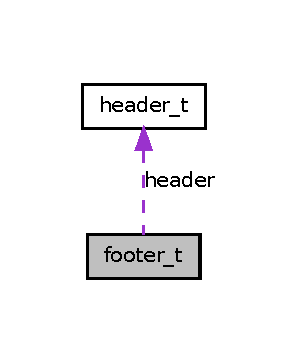
\includegraphics[width=143pt]{structfooter__t__coll__graph}
\end{center}
\end{figure}
\subsection*{Data Fields}
\begin{DoxyCompactItemize}
\item 
\hyperlink{library_8h_ad7ecf93b77285d9bf039d27fa3f1a588}{u32int} \hyperlink{structfooter__t_a5a7b763a121d2c2573df337c8537a6a0}{magic}
\item 
\hyperlink{structheader__t}{header\_\-t} $\ast$ \hyperlink{structfooter__t_aeeb0a5ca163f802e1e3253c0eb9cca88}{header}
\end{DoxyCompactItemize}


\subsection{Field Documentation}
\hypertarget{structfooter__t_aeeb0a5ca163f802e1e3253c0eb9cca88}{
\index{footer\_\-t@{footer\_\-t}!header@{header}}
\index{header@{header}!footer_t@{footer\_\-t}}
\subsubsection[{header}]{\setlength{\rightskip}{0pt plus 5cm}{\bf header\_\-t}$\ast$ {\bf header}}}
\label{structfooter__t_aeeb0a5ca163f802e1e3253c0eb9cca88}
\hypertarget{structfooter__t_a5a7b763a121d2c2573df337c8537a6a0}{
\index{footer\_\-t@{footer\_\-t}!magic@{magic}}
\index{magic@{magic}!footer_t@{footer\_\-t}}
\subsubsection[{magic}]{\setlength{\rightskip}{0pt plus 5cm}{\bf u32int} {\bf magic}}}
\label{structfooter__t_a5a7b763a121d2c2573df337c8537a6a0}


The documentation for this struct was generated from the following file:\begin{DoxyCompactItemize}
\item 
\hyperlink{kmem_8h}{kmem.h}\end{DoxyCompactItemize}

\hypertarget{structgdt__entry}{
\section{gdt\_\-entry Struct Reference}
\label{structgdt__entry}\index{gdt\_\-entry@{gdt\_\-entry}}
}


{\ttfamily \#include $<$descriptor\_\-tables.h$>$}

\subsection*{Data Fields}
\begin{DoxyCompactItemize}
\item 
unsigned short \hyperlink{structgdt__entry_aacba9616b9bdd5895e8dcf5567e4170c}{limit\_\-low}
\item 
unsigned short \hyperlink{structgdt__entry_ae4b82d5bd06e0cad3df76bcabedfe194}{base\_\-low}
\item 
unsigned char \hyperlink{structgdt__entry_a11134ae8e899bd8f22b3d59dd5b86fae}{base\_\-middle}
\item 
unsigned char \hyperlink{structgdt__entry_a1466f288c685860255d8e68192262c44}{access}
\item 
unsigned char \hyperlink{structgdt__entry_a97775c42d71e8858948fa91b472876fb}{granularity}
\item 
unsigned char \hyperlink{structgdt__entry_a2ece4ce625dcee29c9a9e6952055ddd5}{base\_\-high}
\end{DoxyCompactItemize}


\subsection{Field Documentation}
\hypertarget{structgdt__entry_a1466f288c685860255d8e68192262c44}{
\index{gdt\_\-entry@{gdt\_\-entry}!access@{access}}
\index{access@{access}!gdt_entry@{gdt\_\-entry}}
\subsubsection[{access}]{\setlength{\rightskip}{0pt plus 5cm}unsigned char {\bf access}}}
\label{structgdt__entry_a1466f288c685860255d8e68192262c44}
\hypertarget{structgdt__entry_a2ece4ce625dcee29c9a9e6952055ddd5}{
\index{gdt\_\-entry@{gdt\_\-entry}!base\_\-high@{base\_\-high}}
\index{base\_\-high@{base\_\-high}!gdt_entry@{gdt\_\-entry}}
\subsubsection[{base\_\-high}]{\setlength{\rightskip}{0pt plus 5cm}unsigned char {\bf base\_\-high}}}
\label{structgdt__entry_a2ece4ce625dcee29c9a9e6952055ddd5}
\hypertarget{structgdt__entry_ae4b82d5bd06e0cad3df76bcabedfe194}{
\index{gdt\_\-entry@{gdt\_\-entry}!base\_\-low@{base\_\-low}}
\index{base\_\-low@{base\_\-low}!gdt_entry@{gdt\_\-entry}}
\subsubsection[{base\_\-low}]{\setlength{\rightskip}{0pt plus 5cm}unsigned short {\bf base\_\-low}}}
\label{structgdt__entry_ae4b82d5bd06e0cad3df76bcabedfe194}
\hypertarget{structgdt__entry_a11134ae8e899bd8f22b3d59dd5b86fae}{
\index{gdt\_\-entry@{gdt\_\-entry}!base\_\-middle@{base\_\-middle}}
\index{base\_\-middle@{base\_\-middle}!gdt_entry@{gdt\_\-entry}}
\subsubsection[{base\_\-middle}]{\setlength{\rightskip}{0pt plus 5cm}unsigned char {\bf base\_\-middle}}}
\label{structgdt__entry_a11134ae8e899bd8f22b3d59dd5b86fae}
\hypertarget{structgdt__entry_a97775c42d71e8858948fa91b472876fb}{
\index{gdt\_\-entry@{gdt\_\-entry}!granularity@{granularity}}
\index{granularity@{granularity}!gdt_entry@{gdt\_\-entry}}
\subsubsection[{granularity}]{\setlength{\rightskip}{0pt plus 5cm}unsigned char {\bf granularity}}}
\label{structgdt__entry_a97775c42d71e8858948fa91b472876fb}
\hypertarget{structgdt__entry_aacba9616b9bdd5895e8dcf5567e4170c}{
\index{gdt\_\-entry@{gdt\_\-entry}!limit\_\-low@{limit\_\-low}}
\index{limit\_\-low@{limit\_\-low}!gdt_entry@{gdt\_\-entry}}
\subsubsection[{limit\_\-low}]{\setlength{\rightskip}{0pt plus 5cm}unsigned short {\bf limit\_\-low}}}
\label{structgdt__entry_aacba9616b9bdd5895e8dcf5567e4170c}


The documentation for this struct was generated from the following file:\begin{DoxyCompactItemize}
\item 
\hyperlink{descriptor__tables_8h}{descriptor\_\-tables.h}\end{DoxyCompactItemize}

\hypertarget{structgdt__ptr}{
\section{gdt\_\-ptr Struct Reference}
\label{structgdt__ptr}\index{gdt\_\-ptr@{gdt\_\-ptr}}
}


{\ttfamily \#include $<$descriptor\_\-tables.h$>$}

\subsection*{Data Fields}
\begin{DoxyCompactItemize}
\item 
unsigned short \hyperlink{structgdt__ptr_ab50c2dcb9d4a34ea1a5ac52272502379}{limit}
\item 
unsigned int \hyperlink{structgdt__ptr_a2e013c2c6e8010c8116c6f56813df57b}{base}
\end{DoxyCompactItemize}


\subsection{Field Documentation}
\hypertarget{structgdt__ptr_a2e013c2c6e8010c8116c6f56813df57b}{
\index{gdt\_\-ptr@{gdt\_\-ptr}!base@{base}}
\index{base@{base}!gdt_ptr@{gdt\_\-ptr}}
\subsubsection[{base}]{\setlength{\rightskip}{0pt plus 5cm}unsigned int {\bf base}}}
\label{structgdt__ptr_a2e013c2c6e8010c8116c6f56813df57b}
\hypertarget{structgdt__ptr_ab50c2dcb9d4a34ea1a5ac52272502379}{
\index{gdt\_\-ptr@{gdt\_\-ptr}!limit@{limit}}
\index{limit@{limit}!gdt_ptr@{gdt\_\-ptr}}
\subsubsection[{limit}]{\setlength{\rightskip}{0pt plus 5cm}unsigned short {\bf limit}}}
\label{structgdt__ptr_ab50c2dcb9d4a34ea1a5ac52272502379}


The documentation for this struct was generated from the following file:\begin{DoxyCompactItemize}
\item 
\hyperlink{descriptor__tables_8h}{descriptor\_\-tables.h}\end{DoxyCompactItemize}

\hypertarget{structheader__t}{
\section{header\_\-t Struct Reference}
\label{structheader__t}\index{header\_\-t@{header\_\-t}}
}


{\ttfamily \#include $<$kmem.h$>$}

\subsection*{Data Fields}
\begin{DoxyCompactItemize}
\item 
\hyperlink{library_8h_ad7ecf93b77285d9bf039d27fa3f1a588}{u32int} \hyperlink{structheader__t_a5a7b763a121d2c2573df337c8537a6a0}{magic}
\item 
\hyperlink{library_8h_a1026e682ffdadc1701c42cd44ce9efcf}{u8int} \hyperlink{structheader__t_a36d2573383faf36513f89b35327de3cc}{is\_\-hole}
\item 
\hyperlink{library_8h_ad7ecf93b77285d9bf039d27fa3f1a588}{u32int} \hyperlink{structheader__t_a8c5ccb4d457cb24df33a7c9facfa2650}{size}
\end{DoxyCompactItemize}


\subsection{Field Documentation}
\hypertarget{structheader__t_a36d2573383faf36513f89b35327de3cc}{
\index{header\_\-t@{header\_\-t}!is\_\-hole@{is\_\-hole}}
\index{is\_\-hole@{is\_\-hole}!header_t@{header\_\-t}}
\subsubsection[{is\_\-hole}]{\setlength{\rightskip}{0pt plus 5cm}{\bf u8int} {\bf is\_\-hole}}}
\label{structheader__t_a36d2573383faf36513f89b35327de3cc}
\hypertarget{structheader__t_a5a7b763a121d2c2573df337c8537a6a0}{
\index{header\_\-t@{header\_\-t}!magic@{magic}}
\index{magic@{magic}!header_t@{header\_\-t}}
\subsubsection[{magic}]{\setlength{\rightskip}{0pt plus 5cm}{\bf u32int} {\bf magic}}}
\label{structheader__t_a5a7b763a121d2c2573df337c8537a6a0}
\hypertarget{structheader__t_a8c5ccb4d457cb24df33a7c9facfa2650}{
\index{header\_\-t@{header\_\-t}!size@{size}}
\index{size@{size}!header_t@{header\_\-t}}
\subsubsection[{size}]{\setlength{\rightskip}{0pt plus 5cm}{\bf u32int} {\bf size}}}
\label{structheader__t_a8c5ccb4d457cb24df33a7c9facfa2650}


The documentation for this struct was generated from the following file:\begin{DoxyCompactItemize}
\item 
\hyperlink{kmem_8h}{kmem.h}\end{DoxyCompactItemize}

\hypertarget{structheap__t}{
\section{heap\_\-t Struct Reference}
\label{structheap__t}\index{heap\_\-t@{heap\_\-t}}
}


{\ttfamily \#include $<$kmem.h$>$}



Collaboration diagram for heap\_\-t:\nopagebreak
\begin{figure}[H]
\begin{center}
\leavevmode
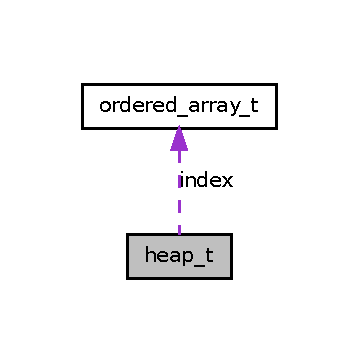
\includegraphics[width=172pt]{structheap__t__coll__graph}
\end{center}
\end{figure}
\subsection*{Data Fields}
\begin{DoxyCompactItemize}
\item 
\hyperlink{structordered__array__t}{ordered\_\-array\_\-t} \hyperlink{structheap__t_a0eef4ef9a0236ead3069bdfd7a1998d4}{index}
\item 
\hyperlink{library_8h_ad7ecf93b77285d9bf039d27fa3f1a588}{u32int} \hyperlink{structheap__t_a82c233a1bbc072e5d6a04b9ec5188648}{start\_\-address}
\item 
\hyperlink{library_8h_ad7ecf93b77285d9bf039d27fa3f1a588}{u32int} \hyperlink{structheap__t_ad770aa56fce7e1ed44266a29def2234e}{end\_\-address}
\item 
\hyperlink{library_8h_ad7ecf93b77285d9bf039d27fa3f1a588}{u32int} \hyperlink{structheap__t_a846e12b614d724a6eddfebe50f200f5a}{max\_\-address}
\item 
\hyperlink{library_8h_a1026e682ffdadc1701c42cd44ce9efcf}{u8int} \hyperlink{structheap__t_adcd96884114847dfe3f1a765b4ee2ecc}{supervisor}
\item 
\hyperlink{library_8h_a1026e682ffdadc1701c42cd44ce9efcf}{u8int} \hyperlink{structheap__t_ae3dd1cfe611a922dc2f36557401a6d8f}{readonly}
\end{DoxyCompactItemize}


\subsection{Field Documentation}
\hypertarget{structheap__t_ad770aa56fce7e1ed44266a29def2234e}{
\index{heap\_\-t@{heap\_\-t}!end\_\-address@{end\_\-address}}
\index{end\_\-address@{end\_\-address}!heap_t@{heap\_\-t}}
\subsubsection[{end\_\-address}]{\setlength{\rightskip}{0pt plus 5cm}{\bf u32int} {\bf end\_\-address}}}
\label{structheap__t_ad770aa56fce7e1ed44266a29def2234e}
\hypertarget{structheap__t_a0eef4ef9a0236ead3069bdfd7a1998d4}{
\index{heap\_\-t@{heap\_\-t}!index@{index}}
\index{index@{index}!heap_t@{heap\_\-t}}
\subsubsection[{index}]{\setlength{\rightskip}{0pt plus 5cm}{\bf ordered\_\-array\_\-t} {\bf index}}}
\label{structheap__t_a0eef4ef9a0236ead3069bdfd7a1998d4}
\hypertarget{structheap__t_a846e12b614d724a6eddfebe50f200f5a}{
\index{heap\_\-t@{heap\_\-t}!max\_\-address@{max\_\-address}}
\index{max\_\-address@{max\_\-address}!heap_t@{heap\_\-t}}
\subsubsection[{max\_\-address}]{\setlength{\rightskip}{0pt plus 5cm}{\bf u32int} {\bf max\_\-address}}}
\label{structheap__t_a846e12b614d724a6eddfebe50f200f5a}
\hypertarget{structheap__t_ae3dd1cfe611a922dc2f36557401a6d8f}{
\index{heap\_\-t@{heap\_\-t}!readonly@{readonly}}
\index{readonly@{readonly}!heap_t@{heap\_\-t}}
\subsubsection[{readonly}]{\setlength{\rightskip}{0pt plus 5cm}{\bf u8int} {\bf readonly}}}
\label{structheap__t_ae3dd1cfe611a922dc2f36557401a6d8f}
\hypertarget{structheap__t_a82c233a1bbc072e5d6a04b9ec5188648}{
\index{heap\_\-t@{heap\_\-t}!start\_\-address@{start\_\-address}}
\index{start\_\-address@{start\_\-address}!heap_t@{heap\_\-t}}
\subsubsection[{start\_\-address}]{\setlength{\rightskip}{0pt plus 5cm}{\bf u32int} {\bf start\_\-address}}}
\label{structheap__t_a82c233a1bbc072e5d6a04b9ec5188648}
\hypertarget{structheap__t_adcd96884114847dfe3f1a765b4ee2ecc}{
\index{heap\_\-t@{heap\_\-t}!supervisor@{supervisor}}
\index{supervisor@{supervisor}!heap_t@{heap\_\-t}}
\subsubsection[{supervisor}]{\setlength{\rightskip}{0pt plus 5cm}{\bf u8int} {\bf supervisor}}}
\label{structheap__t_adcd96884114847dfe3f1a765b4ee2ecc}


The documentation for this struct was generated from the following file:\begin{DoxyCompactItemize}
\item 
\hyperlink{kmem_8h}{kmem.h}\end{DoxyCompactItemize}

\hypertarget{structidt__entry__struct}{
\section{idt\_\-entry\_\-struct Struct Reference}
\label{structidt__entry__struct}\index{idt\_\-entry\_\-struct@{idt\_\-entry\_\-struct}}
}


{\ttfamily \#include $<$descriptor\_\-tables.h$>$}

\subsection*{Data Fields}
\begin{DoxyCompactItemize}
\item 
\hyperlink{library_8h_a863d9497073aad2b991aeab2211d87af}{u16int} \hyperlink{structidt__entry__struct_a87eb3dc5d98a750439e08c9e6703778b}{base\_\-lo}
\item 
\hyperlink{library_8h_a863d9497073aad2b991aeab2211d87af}{u16int} \hyperlink{structidt__entry__struct_adf6a7546c6355a8f87f34731860b49e1}{sel}
\item 
\hyperlink{library_8h_a1026e682ffdadc1701c42cd44ce9efcf}{u8int} \hyperlink{structidt__entry__struct_a9d3c870e7b1697c835095c536ac5b09b}{always0}
\item 
\hyperlink{library_8h_a1026e682ffdadc1701c42cd44ce9efcf}{u8int} \hyperlink{structidt__entry__struct_a138dda98fcd4738346af61bcca8cf4b4}{flags}
\item 
\hyperlink{library_8h_a863d9497073aad2b991aeab2211d87af}{u16int} \hyperlink{structidt__entry__struct_a65b35eebe0d81928a3ac5ddb1efe0fc3}{base\_\-hi}
\end{DoxyCompactItemize}


\subsection{Field Documentation}
\hypertarget{structidt__entry__struct_a9d3c870e7b1697c835095c536ac5b09b}{
\index{idt\_\-entry\_\-struct@{idt\_\-entry\_\-struct}!always0@{always0}}
\index{always0@{always0}!idt_entry_struct@{idt\_\-entry\_\-struct}}
\subsubsection[{always0}]{\setlength{\rightskip}{0pt plus 5cm}{\bf u8int} {\bf always0}}}
\label{structidt__entry__struct_a9d3c870e7b1697c835095c536ac5b09b}
\hypertarget{structidt__entry__struct_a65b35eebe0d81928a3ac5ddb1efe0fc3}{
\index{idt\_\-entry\_\-struct@{idt\_\-entry\_\-struct}!base\_\-hi@{base\_\-hi}}
\index{base\_\-hi@{base\_\-hi}!idt_entry_struct@{idt\_\-entry\_\-struct}}
\subsubsection[{base\_\-hi}]{\setlength{\rightskip}{0pt plus 5cm}{\bf u16int} {\bf base\_\-hi}}}
\label{structidt__entry__struct_a65b35eebe0d81928a3ac5ddb1efe0fc3}
\hypertarget{structidt__entry__struct_a87eb3dc5d98a750439e08c9e6703778b}{
\index{idt\_\-entry\_\-struct@{idt\_\-entry\_\-struct}!base\_\-lo@{base\_\-lo}}
\index{base\_\-lo@{base\_\-lo}!idt_entry_struct@{idt\_\-entry\_\-struct}}
\subsubsection[{base\_\-lo}]{\setlength{\rightskip}{0pt plus 5cm}{\bf u16int} {\bf base\_\-lo}}}
\label{structidt__entry__struct_a87eb3dc5d98a750439e08c9e6703778b}
\hypertarget{structidt__entry__struct_a138dda98fcd4738346af61bcca8cf4b4}{
\index{idt\_\-entry\_\-struct@{idt\_\-entry\_\-struct}!flags@{flags}}
\index{flags@{flags}!idt_entry_struct@{idt\_\-entry\_\-struct}}
\subsubsection[{flags}]{\setlength{\rightskip}{0pt plus 5cm}{\bf u8int} {\bf flags}}}
\label{structidt__entry__struct_a138dda98fcd4738346af61bcca8cf4b4}
\hypertarget{structidt__entry__struct_adf6a7546c6355a8f87f34731860b49e1}{
\index{idt\_\-entry\_\-struct@{idt\_\-entry\_\-struct}!sel@{sel}}
\index{sel@{sel}!idt_entry_struct@{idt\_\-entry\_\-struct}}
\subsubsection[{sel}]{\setlength{\rightskip}{0pt plus 5cm}{\bf u16int} {\bf sel}}}
\label{structidt__entry__struct_adf6a7546c6355a8f87f34731860b49e1}


The documentation for this struct was generated from the following file:\begin{DoxyCompactItemize}
\item 
\hyperlink{descriptor__tables_8h}{descriptor\_\-tables.h}\end{DoxyCompactItemize}

\hypertarget{structidt__ptr__struct}{
\section{idt\_\-ptr\_\-struct Struct Reference}
\label{structidt__ptr__struct}\index{idt\_\-ptr\_\-struct@{idt\_\-ptr\_\-struct}}
}


{\ttfamily \#include $<$descriptor\_\-tables.h$>$}

\subsection*{Data Fields}
\begin{DoxyCompactItemize}
\item 
\hyperlink{library_8h_a863d9497073aad2b991aeab2211d87af}{u16int} \hyperlink{structidt__ptr__struct_a68fd3b4f6c14a331ca9b226cbf122e13}{limit}
\item 
\hyperlink{library_8h_ad7ecf93b77285d9bf039d27fa3f1a588}{u32int} \hyperlink{structidt__ptr__struct_ab5763c2b18c825c8b8fba44b2e60ddc1}{base}
\end{DoxyCompactItemize}


\subsection{Field Documentation}
\hypertarget{structidt__ptr__struct_ab5763c2b18c825c8b8fba44b2e60ddc1}{
\index{idt\_\-ptr\_\-struct@{idt\_\-ptr\_\-struct}!base@{base}}
\index{base@{base}!idt_ptr_struct@{idt\_\-ptr\_\-struct}}
\subsubsection[{base}]{\setlength{\rightskip}{0pt plus 5cm}{\bf u32int} {\bf base}}}
\label{structidt__ptr__struct_ab5763c2b18c825c8b8fba44b2e60ddc1}
\hypertarget{structidt__ptr__struct_a68fd3b4f6c14a331ca9b226cbf122e13}{
\index{idt\_\-ptr\_\-struct@{idt\_\-ptr\_\-struct}!limit@{limit}}
\index{limit@{limit}!idt_ptr_struct@{idt\_\-ptr\_\-struct}}
\subsubsection[{limit}]{\setlength{\rightskip}{0pt plus 5cm}{\bf u16int} {\bf limit}}}
\label{structidt__ptr__struct_a68fd3b4f6c14a331ca9b226cbf122e13}


The documentation for this struct was generated from the following file:\begin{DoxyCompactItemize}
\item 
\hyperlink{descriptor__tables_8h}{descriptor\_\-tables.h}\end{DoxyCompactItemize}

\hypertarget{structinitrd__file__header}{
\section{initrd\_\-file\_\-header Struct Reference}
\label{structinitrd__file__header}\index{initrd\_\-file\_\-header@{initrd\_\-file\_\-header}}
}


{\ttfamily \#include $<$initrd.h$>$}

\subsection*{Data Fields}
\begin{DoxyCompactItemize}
\item 
\hyperlink{library_8h_a1026e682ffdadc1701c42cd44ce9efcf}{u8int} \hyperlink{structinitrd__file__header_a04da1f4036c5c1453e6f6b9c8656ae1c}{magic}
\item 
\hyperlink{library_8h_afa805b2bbcb6f0e85de57cef336f98df}{s8int} \hyperlink{structinitrd__file__header_a9ae4535aa9418230183438e85d054c9b}{name} \mbox{[}64\mbox{]}
\item 
\hyperlink{library_8h_ad7ecf93b77285d9bf039d27fa3f1a588}{u32int} \hyperlink{structinitrd__file__header_aa1d165d830b3ec7f9523dcb357883cb9}{offset}
\item 
\hyperlink{library_8h_ad7ecf93b77285d9bf039d27fa3f1a588}{u32int} \hyperlink{structinitrd__file__header_aeec37a8314ab06b3088adcc9ae433fa4}{length}
\end{DoxyCompactItemize}


\subsection{Field Documentation}
\hypertarget{structinitrd__file__header_aeec37a8314ab06b3088adcc9ae433fa4}{
\index{initrd\_\-file\_\-header@{initrd\_\-file\_\-header}!length@{length}}
\index{length@{length}!initrd_file_header@{initrd\_\-file\_\-header}}
\subsubsection[{length}]{\setlength{\rightskip}{0pt plus 5cm}{\bf u32int} {\bf length}}}
\label{structinitrd__file__header_aeec37a8314ab06b3088adcc9ae433fa4}
\hypertarget{structinitrd__file__header_a04da1f4036c5c1453e6f6b9c8656ae1c}{
\index{initrd\_\-file\_\-header@{initrd\_\-file\_\-header}!magic@{magic}}
\index{magic@{magic}!initrd_file_header@{initrd\_\-file\_\-header}}
\subsubsection[{magic}]{\setlength{\rightskip}{0pt plus 5cm}{\bf u8int} {\bf magic}}}
\label{structinitrd__file__header_a04da1f4036c5c1453e6f6b9c8656ae1c}
\hypertarget{structinitrd__file__header_a9ae4535aa9418230183438e85d054c9b}{
\index{initrd\_\-file\_\-header@{initrd\_\-file\_\-header}!name@{name}}
\index{name@{name}!initrd_file_header@{initrd\_\-file\_\-header}}
\subsubsection[{name}]{\setlength{\rightskip}{0pt plus 5cm}{\bf s8int} {\bf name}\mbox{[}64\mbox{]}}}
\label{structinitrd__file__header_a9ae4535aa9418230183438e85d054c9b}
\hypertarget{structinitrd__file__header_aa1d165d830b3ec7f9523dcb357883cb9}{
\index{initrd\_\-file\_\-header@{initrd\_\-file\_\-header}!offset@{offset}}
\index{offset@{offset}!initrd_file_header@{initrd\_\-file\_\-header}}
\subsubsection[{offset}]{\setlength{\rightskip}{0pt plus 5cm}{\bf u32int} {\bf offset}}}
\label{structinitrd__file__header_aa1d165d830b3ec7f9523dcb357883cb9}


The documentation for this struct was generated from the following file:\begin{DoxyCompactItemize}
\item 
\hyperlink{initrd_8h}{initrd.h}\end{DoxyCompactItemize}

\hypertarget{structinitrd__header}{
\section{initrd\_\-header Struct Reference}
\label{structinitrd__header}\index{initrd\_\-header@{initrd\_\-header}}
}


{\ttfamily \#include $<$initrd.h$>$}

\subsection*{Data Fields}
\begin{DoxyCompactItemize}
\item 
\hyperlink{library_8h_ad7ecf93b77285d9bf039d27fa3f1a588}{u32int} \hyperlink{structinitrd__header_a56ba3190366248af937cdd79cc6efa6e}{nfiles}
\end{DoxyCompactItemize}


\subsection{Field Documentation}
\hypertarget{structinitrd__header_a56ba3190366248af937cdd79cc6efa6e}{
\index{initrd\_\-header@{initrd\_\-header}!nfiles@{nfiles}}
\index{nfiles@{nfiles}!initrd_header@{initrd\_\-header}}
\subsubsection[{nfiles}]{\setlength{\rightskip}{0pt plus 5cm}{\bf u32int} {\bf nfiles}}}
\label{structinitrd__header_a56ba3190366248af937cdd79cc6efa6e}


The documentation for this struct was generated from the following file:\begin{DoxyCompactItemize}
\item 
\hyperlink{initrd_8h}{initrd.h}\end{DoxyCompactItemize}

\hypertarget{structmultiboot}{
\section{multiboot Struct Reference}
\label{structmultiboot}\index{multiboot@{multiboot}}
}


{\ttfamily \#include $<$multiboot.h$>$}

\subsection*{Data Fields}
\begin{DoxyCompactItemize}
\item 
\hyperlink{library_8h_ad7ecf93b77285d9bf039d27fa3f1a588}{u32int} \hyperlink{structmultiboot_a3c67431132e70c431fbfc3bf03a63dd4}{flags}
\item 
\hyperlink{library_8h_ad7ecf93b77285d9bf039d27fa3f1a588}{u32int} \hyperlink{structmultiboot_a2e26dd5cb6e6ff946d30339b5dd1969d}{mem\_\-lower}
\item 
\hyperlink{library_8h_ad7ecf93b77285d9bf039d27fa3f1a588}{u32int} \hyperlink{structmultiboot_a812f64d9a61cbd147d74184fb27cf4fd}{mem\_\-upper}
\item 
\hyperlink{library_8h_ad7ecf93b77285d9bf039d27fa3f1a588}{u32int} \hyperlink{structmultiboot_a38d97031da6dcf05d32af63d0f559f83}{boot\_\-device}
\item 
\hyperlink{library_8h_ad7ecf93b77285d9bf039d27fa3f1a588}{u32int} \hyperlink{structmultiboot_a94e0737ae00bddbac4422634b072ed29}{cmdline}
\item 
\hyperlink{library_8h_ad7ecf93b77285d9bf039d27fa3f1a588}{u32int} \hyperlink{structmultiboot_a4583c5566a915d416ad288ecda27821c}{mods\_\-count}
\item 
\hyperlink{library_8h_ad7ecf93b77285d9bf039d27fa3f1a588}{u32int} \hyperlink{structmultiboot_a94ec60a30a04b4f3d4e259805088b3ba}{mods\_\-addr}
\item 
\hyperlink{library_8h_ad7ecf93b77285d9bf039d27fa3f1a588}{u32int} \hyperlink{structmultiboot_ad359bb84532ae5a74868eb669d4e4cac}{num}
\item 
\hyperlink{library_8h_ad7ecf93b77285d9bf039d27fa3f1a588}{u32int} \hyperlink{structmultiboot_a8c5ccb4d457cb24df33a7c9facfa2650}{size}
\item 
\hyperlink{library_8h_ad7ecf93b77285d9bf039d27fa3f1a588}{u32int} \hyperlink{structmultiboot_a48f994dfe1a5aea3bce6dc7d2be8efd5}{addr}
\item 
\hyperlink{library_8h_ad7ecf93b77285d9bf039d27fa3f1a588}{u32int} \hyperlink{structmultiboot_adde24ffd0b3acf092bc1776da5c15815}{shndx}
\item 
\hyperlink{library_8h_ad7ecf93b77285d9bf039d27fa3f1a588}{u32int} \hyperlink{structmultiboot_a0d2c0c8d20e751f9a48a40e8b614abe0}{mmap\_\-length}
\item 
\hyperlink{library_8h_ad7ecf93b77285d9bf039d27fa3f1a588}{u32int} \hyperlink{structmultiboot_a59f139d6f94af6b1d1afeae3b3ca5384}{mmap\_\-addr}
\item 
\hyperlink{library_8h_ad7ecf93b77285d9bf039d27fa3f1a588}{u32int} \hyperlink{structmultiboot_a60d4345d5d99f09989db441b216e8522}{drives\_\-length}
\item 
\hyperlink{library_8h_ad7ecf93b77285d9bf039d27fa3f1a588}{u32int} \hyperlink{structmultiboot_aabb292b14d3d3a5dc9fc784326dae29d}{drives\_\-addr}
\item 
\hyperlink{library_8h_ad7ecf93b77285d9bf039d27fa3f1a588}{u32int} \hyperlink{structmultiboot_a1cbecf19c3d7f0b580787509c37d03ea}{config\_\-table}
\item 
\hyperlink{library_8h_ad7ecf93b77285d9bf039d27fa3f1a588}{u32int} \hyperlink{structmultiboot_aae2d904da246801c7b2517cb68277ecd}{boot\_\-loader\_\-name}
\item 
\hyperlink{library_8h_ad7ecf93b77285d9bf039d27fa3f1a588}{u32int} \hyperlink{structmultiboot_a4798878e2abd581297b1b7f080a92c72}{apm\_\-table}
\item 
\hyperlink{library_8h_ad7ecf93b77285d9bf039d27fa3f1a588}{u32int} \hyperlink{structmultiboot_a6c6976dc3eb7273c6ebbba74f00bcdfd}{vbe\_\-control\_\-info}
\item 
\hyperlink{library_8h_ad7ecf93b77285d9bf039d27fa3f1a588}{u32int} \hyperlink{structmultiboot_abfceba4fe6886ce70184ca01f67155cc}{vbe\_\-mode\_\-info}
\item 
\hyperlink{library_8h_ad7ecf93b77285d9bf039d27fa3f1a588}{u32int} \hyperlink{structmultiboot_aaca371d7e671a0f6da3fe7f9786a49df}{vbe\_\-mode}
\item 
\hyperlink{library_8h_ad7ecf93b77285d9bf039d27fa3f1a588}{u32int} \hyperlink{structmultiboot_a107829766e01a5c0f724f78284b84310}{vbe\_\-interface\_\-seg}
\item 
\hyperlink{library_8h_ad7ecf93b77285d9bf039d27fa3f1a588}{u32int} \hyperlink{structmultiboot_a3e50caa9e879f6cbe6915a06f4ab9515}{vbe\_\-interface\_\-off}
\item 
\hyperlink{library_8h_ad7ecf93b77285d9bf039d27fa3f1a588}{u32int} \hyperlink{structmultiboot_a384b5cb6672109480ce43374e0d06ecb}{vbe\_\-interface\_\-len}
\end{DoxyCompactItemize}


\subsection{Field Documentation}
\hypertarget{structmultiboot_a48f994dfe1a5aea3bce6dc7d2be8efd5}{
\index{multiboot@{multiboot}!addr@{addr}}
\index{addr@{addr}!multiboot@{multiboot}}
\subsubsection[{addr}]{\setlength{\rightskip}{0pt plus 5cm}{\bf u32int} {\bf addr}}}
\label{structmultiboot_a48f994dfe1a5aea3bce6dc7d2be8efd5}
\hypertarget{structmultiboot_a4798878e2abd581297b1b7f080a92c72}{
\index{multiboot@{multiboot}!apm\_\-table@{apm\_\-table}}
\index{apm\_\-table@{apm\_\-table}!multiboot@{multiboot}}
\subsubsection[{apm\_\-table}]{\setlength{\rightskip}{0pt plus 5cm}{\bf u32int} {\bf apm\_\-table}}}
\label{structmultiboot_a4798878e2abd581297b1b7f080a92c72}
\hypertarget{structmultiboot_a38d97031da6dcf05d32af63d0f559f83}{
\index{multiboot@{multiboot}!boot\_\-device@{boot\_\-device}}
\index{boot\_\-device@{boot\_\-device}!multiboot@{multiboot}}
\subsubsection[{boot\_\-device}]{\setlength{\rightskip}{0pt plus 5cm}{\bf u32int} {\bf boot\_\-device}}}
\label{structmultiboot_a38d97031da6dcf05d32af63d0f559f83}
\hypertarget{structmultiboot_aae2d904da246801c7b2517cb68277ecd}{
\index{multiboot@{multiboot}!boot\_\-loader\_\-name@{boot\_\-loader\_\-name}}
\index{boot\_\-loader\_\-name@{boot\_\-loader\_\-name}!multiboot@{multiboot}}
\subsubsection[{boot\_\-loader\_\-name}]{\setlength{\rightskip}{0pt plus 5cm}{\bf u32int} {\bf boot\_\-loader\_\-name}}}
\label{structmultiboot_aae2d904da246801c7b2517cb68277ecd}
\hypertarget{structmultiboot_a94e0737ae00bddbac4422634b072ed29}{
\index{multiboot@{multiboot}!cmdline@{cmdline}}
\index{cmdline@{cmdline}!multiboot@{multiboot}}
\subsubsection[{cmdline}]{\setlength{\rightskip}{0pt plus 5cm}{\bf u32int} {\bf cmdline}}}
\label{structmultiboot_a94e0737ae00bddbac4422634b072ed29}
\hypertarget{structmultiboot_a1cbecf19c3d7f0b580787509c37d03ea}{
\index{multiboot@{multiboot}!config\_\-table@{config\_\-table}}
\index{config\_\-table@{config\_\-table}!multiboot@{multiboot}}
\subsubsection[{config\_\-table}]{\setlength{\rightskip}{0pt plus 5cm}{\bf u32int} {\bf config\_\-table}}}
\label{structmultiboot_a1cbecf19c3d7f0b580787509c37d03ea}
\hypertarget{structmultiboot_aabb292b14d3d3a5dc9fc784326dae29d}{
\index{multiboot@{multiboot}!drives\_\-addr@{drives\_\-addr}}
\index{drives\_\-addr@{drives\_\-addr}!multiboot@{multiboot}}
\subsubsection[{drives\_\-addr}]{\setlength{\rightskip}{0pt plus 5cm}{\bf u32int} {\bf drives\_\-addr}}}
\label{structmultiboot_aabb292b14d3d3a5dc9fc784326dae29d}
\hypertarget{structmultiboot_a60d4345d5d99f09989db441b216e8522}{
\index{multiboot@{multiboot}!drives\_\-length@{drives\_\-length}}
\index{drives\_\-length@{drives\_\-length}!multiboot@{multiboot}}
\subsubsection[{drives\_\-length}]{\setlength{\rightskip}{0pt plus 5cm}{\bf u32int} {\bf drives\_\-length}}}
\label{structmultiboot_a60d4345d5d99f09989db441b216e8522}
\hypertarget{structmultiboot_a3c67431132e70c431fbfc3bf03a63dd4}{
\index{multiboot@{multiboot}!flags@{flags}}
\index{flags@{flags}!multiboot@{multiboot}}
\subsubsection[{flags}]{\setlength{\rightskip}{0pt plus 5cm}{\bf u32int} {\bf flags}}}
\label{structmultiboot_a3c67431132e70c431fbfc3bf03a63dd4}
\hypertarget{structmultiboot_a2e26dd5cb6e6ff946d30339b5dd1969d}{
\index{multiboot@{multiboot}!mem\_\-lower@{mem\_\-lower}}
\index{mem\_\-lower@{mem\_\-lower}!multiboot@{multiboot}}
\subsubsection[{mem\_\-lower}]{\setlength{\rightskip}{0pt plus 5cm}{\bf u32int} {\bf mem\_\-lower}}}
\label{structmultiboot_a2e26dd5cb6e6ff946d30339b5dd1969d}
\hypertarget{structmultiboot_a812f64d9a61cbd147d74184fb27cf4fd}{
\index{multiboot@{multiboot}!mem\_\-upper@{mem\_\-upper}}
\index{mem\_\-upper@{mem\_\-upper}!multiboot@{multiboot}}
\subsubsection[{mem\_\-upper}]{\setlength{\rightskip}{0pt plus 5cm}{\bf u32int} {\bf mem\_\-upper}}}
\label{structmultiboot_a812f64d9a61cbd147d74184fb27cf4fd}
\hypertarget{structmultiboot_a59f139d6f94af6b1d1afeae3b3ca5384}{
\index{multiboot@{multiboot}!mmap\_\-addr@{mmap\_\-addr}}
\index{mmap\_\-addr@{mmap\_\-addr}!multiboot@{multiboot}}
\subsubsection[{mmap\_\-addr}]{\setlength{\rightskip}{0pt plus 5cm}{\bf u32int} {\bf mmap\_\-addr}}}
\label{structmultiboot_a59f139d6f94af6b1d1afeae3b3ca5384}
\hypertarget{structmultiboot_a0d2c0c8d20e751f9a48a40e8b614abe0}{
\index{multiboot@{multiboot}!mmap\_\-length@{mmap\_\-length}}
\index{mmap\_\-length@{mmap\_\-length}!multiboot@{multiboot}}
\subsubsection[{mmap\_\-length}]{\setlength{\rightskip}{0pt plus 5cm}{\bf u32int} {\bf mmap\_\-length}}}
\label{structmultiboot_a0d2c0c8d20e751f9a48a40e8b614abe0}
\hypertarget{structmultiboot_a94ec60a30a04b4f3d4e259805088b3ba}{
\index{multiboot@{multiboot}!mods\_\-addr@{mods\_\-addr}}
\index{mods\_\-addr@{mods\_\-addr}!multiboot@{multiboot}}
\subsubsection[{mods\_\-addr}]{\setlength{\rightskip}{0pt plus 5cm}{\bf u32int} {\bf mods\_\-addr}}}
\label{structmultiboot_a94ec60a30a04b4f3d4e259805088b3ba}
\hypertarget{structmultiboot_a4583c5566a915d416ad288ecda27821c}{
\index{multiboot@{multiboot}!mods\_\-count@{mods\_\-count}}
\index{mods\_\-count@{mods\_\-count}!multiboot@{multiboot}}
\subsubsection[{mods\_\-count}]{\setlength{\rightskip}{0pt plus 5cm}{\bf u32int} {\bf mods\_\-count}}}
\label{structmultiboot_a4583c5566a915d416ad288ecda27821c}
\hypertarget{structmultiboot_ad359bb84532ae5a74868eb669d4e4cac}{
\index{multiboot@{multiboot}!num@{num}}
\index{num@{num}!multiboot@{multiboot}}
\subsubsection[{num}]{\setlength{\rightskip}{0pt plus 5cm}{\bf u32int} {\bf num}}}
\label{structmultiboot_ad359bb84532ae5a74868eb669d4e4cac}
\hypertarget{structmultiboot_adde24ffd0b3acf092bc1776da5c15815}{
\index{multiboot@{multiboot}!shndx@{shndx}}
\index{shndx@{shndx}!multiboot@{multiboot}}
\subsubsection[{shndx}]{\setlength{\rightskip}{0pt plus 5cm}{\bf u32int} {\bf shndx}}}
\label{structmultiboot_adde24ffd0b3acf092bc1776da5c15815}
\hypertarget{structmultiboot_a8c5ccb4d457cb24df33a7c9facfa2650}{
\index{multiboot@{multiboot}!size@{size}}
\index{size@{size}!multiboot@{multiboot}}
\subsubsection[{size}]{\setlength{\rightskip}{0pt plus 5cm}{\bf u32int} {\bf size}}}
\label{structmultiboot_a8c5ccb4d457cb24df33a7c9facfa2650}
\hypertarget{structmultiboot_a6c6976dc3eb7273c6ebbba74f00bcdfd}{
\index{multiboot@{multiboot}!vbe\_\-control\_\-info@{vbe\_\-control\_\-info}}
\index{vbe\_\-control\_\-info@{vbe\_\-control\_\-info}!multiboot@{multiboot}}
\subsubsection[{vbe\_\-control\_\-info}]{\setlength{\rightskip}{0pt plus 5cm}{\bf u32int} {\bf vbe\_\-control\_\-info}}}
\label{structmultiboot_a6c6976dc3eb7273c6ebbba74f00bcdfd}
\hypertarget{structmultiboot_a384b5cb6672109480ce43374e0d06ecb}{
\index{multiboot@{multiboot}!vbe\_\-interface\_\-len@{vbe\_\-interface\_\-len}}
\index{vbe\_\-interface\_\-len@{vbe\_\-interface\_\-len}!multiboot@{multiboot}}
\subsubsection[{vbe\_\-interface\_\-len}]{\setlength{\rightskip}{0pt plus 5cm}{\bf u32int} {\bf vbe\_\-interface\_\-len}}}
\label{structmultiboot_a384b5cb6672109480ce43374e0d06ecb}
\hypertarget{structmultiboot_a3e50caa9e879f6cbe6915a06f4ab9515}{
\index{multiboot@{multiboot}!vbe\_\-interface\_\-off@{vbe\_\-interface\_\-off}}
\index{vbe\_\-interface\_\-off@{vbe\_\-interface\_\-off}!multiboot@{multiboot}}
\subsubsection[{vbe\_\-interface\_\-off}]{\setlength{\rightskip}{0pt plus 5cm}{\bf u32int} {\bf vbe\_\-interface\_\-off}}}
\label{structmultiboot_a3e50caa9e879f6cbe6915a06f4ab9515}
\hypertarget{structmultiboot_a107829766e01a5c0f724f78284b84310}{
\index{multiboot@{multiboot}!vbe\_\-interface\_\-seg@{vbe\_\-interface\_\-seg}}
\index{vbe\_\-interface\_\-seg@{vbe\_\-interface\_\-seg}!multiboot@{multiboot}}
\subsubsection[{vbe\_\-interface\_\-seg}]{\setlength{\rightskip}{0pt plus 5cm}{\bf u32int} {\bf vbe\_\-interface\_\-seg}}}
\label{structmultiboot_a107829766e01a5c0f724f78284b84310}
\hypertarget{structmultiboot_aaca371d7e671a0f6da3fe7f9786a49df}{
\index{multiboot@{multiboot}!vbe\_\-mode@{vbe\_\-mode}}
\index{vbe\_\-mode@{vbe\_\-mode}!multiboot@{multiboot}}
\subsubsection[{vbe\_\-mode}]{\setlength{\rightskip}{0pt plus 5cm}{\bf u32int} {\bf vbe\_\-mode}}}
\label{structmultiboot_aaca371d7e671a0f6da3fe7f9786a49df}
\hypertarget{structmultiboot_abfceba4fe6886ce70184ca01f67155cc}{
\index{multiboot@{multiboot}!vbe\_\-mode\_\-info@{vbe\_\-mode\_\-info}}
\index{vbe\_\-mode\_\-info@{vbe\_\-mode\_\-info}!multiboot@{multiboot}}
\subsubsection[{vbe\_\-mode\_\-info}]{\setlength{\rightskip}{0pt plus 5cm}{\bf u32int} {\bf vbe\_\-mode\_\-info}}}
\label{structmultiboot_abfceba4fe6886ce70184ca01f67155cc}


The documentation for this struct was generated from the following file:\begin{DoxyCompactItemize}
\item 
\hyperlink{multiboot_8h}{multiboot.h}\end{DoxyCompactItemize}

\hypertarget{structnode}{
\section{node Struct Reference}
\label{structnode}\index{node@{node}}
}


{\ttfamily \#include $<$fs.h$>$}



Collaboration diagram for node:\nopagebreak
\begin{figure}[H]
\begin{center}
\leavevmode
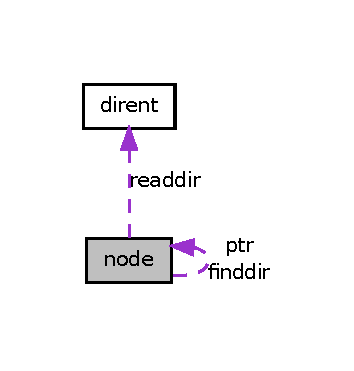
\includegraphics[width=170pt]{structnode__coll__graph}
\end{center}
\end{figure}
\subsection*{Data Fields}
\begin{DoxyCompactItemize}
\item 
char \hyperlink{structnode_a93a4209b66c75fd711969ba8dcd926f5}{name} \mbox{[}128\mbox{]}
\item 
\hyperlink{library_8h_ad7ecf93b77285d9bf039d27fa3f1a588}{u32int} \hyperlink{structnode_aacc3e3dee374838b98a0b76a85feb721}{mask}
\item 
\hyperlink{library_8h_ad7ecf93b77285d9bf039d27fa3f1a588}{u32int} \hyperlink{structnode_a1e5520ef7304cc522418c540d561c0a3}{uid}
\item 
\hyperlink{library_8h_ad7ecf93b77285d9bf039d27fa3f1a588}{u32int} \hyperlink{structnode_adc4a5165896c5347e088f15bc93ff8dc}{gid}
\item 
\hyperlink{library_8h_ad7ecf93b77285d9bf039d27fa3f1a588}{u32int} \hyperlink{structnode_a3c67431132e70c431fbfc3bf03a63dd4}{flags}
\item 
\hyperlink{library_8h_ad7ecf93b77285d9bf039d27fa3f1a588}{u32int} \hyperlink{structnode_a1ea843802457b0d31c6d2d2d5c662077}{inode}
\item 
\hyperlink{library_8h_ad7ecf93b77285d9bf039d27fa3f1a588}{u32int} \hyperlink{structnode_aeec37a8314ab06b3088adcc9ae433fa4}{length}
\item 
\hyperlink{library_8h_ad7ecf93b77285d9bf039d27fa3f1a588}{u32int} \hyperlink{structnode_ae55321901d1853c575f21b4e7256ede6}{impl}
\item 
\hyperlink{fs_8h_ad32b9ac667034d4edf8dc6a9e5306642}{read\_\-type\_\-t} \hyperlink{structnode_a05ab3f286863dee95791cdf95562b35e}{read}
\item 
\hyperlink{fs_8h_afbbf89d19d9d2ef84997351f4af5ea2f}{write\_\-type\_\-t} \hyperlink{structnode_a2441fff861fbd77a313d39d7d53b92e4}{write}
\item 
\hyperlink{fs_8h_a0ef1927acc994d2ab9608eb4eb4308c6}{open\_\-type\_\-t} \hyperlink{structnode_a4f99008a4bc4cd624c4f25e27851b48a}{open}
\item 
\hyperlink{fs_8h_aff25a2dc065528aaedb6e2c21cbc7659}{close\_\-type\_\-t} \hyperlink{structnode_aa53bc19f51782a3a27defe2d22e1bd0d}{close}
\item 
\hyperlink{fs_8h_a654cc2a1ada446257b3ef6ac2c1ea7c8}{readdir\_\-type\_\-t} \hyperlink{structnode_adfc053274b205b3218ef061345cbd899}{readdir}
\item 
\hyperlink{fs_8h_a9961273780df33e576ff4063800f23b4}{finddir\_\-type\_\-t} \hyperlink{structnode_a1721355afe8d778d82355f2b29ee5f8e}{finddir}
\item 
struct \hyperlink{structnode}{node} $\ast$ \hyperlink{structnode_afaf6d285cebe95dd6208a3b509d394a4}{ptr}
\end{DoxyCompactItemize}


\subsection{Field Documentation}
\hypertarget{structnode_aa53bc19f51782a3a27defe2d22e1bd0d}{
\index{node@{node}!close@{close}}
\index{close@{close}!node@{node}}
\subsubsection[{close}]{\setlength{\rightskip}{0pt plus 5cm}{\bf close\_\-type\_\-t} {\bf close}}}
\label{structnode_aa53bc19f51782a3a27defe2d22e1bd0d}
\hypertarget{structnode_a1721355afe8d778d82355f2b29ee5f8e}{
\index{node@{node}!finddir@{finddir}}
\index{finddir@{finddir}!node@{node}}
\subsubsection[{finddir}]{\setlength{\rightskip}{0pt plus 5cm}{\bf finddir\_\-type\_\-t} {\bf finddir}}}
\label{structnode_a1721355afe8d778d82355f2b29ee5f8e}
\hypertarget{structnode_a3c67431132e70c431fbfc3bf03a63dd4}{
\index{node@{node}!flags@{flags}}
\index{flags@{flags}!node@{node}}
\subsubsection[{flags}]{\setlength{\rightskip}{0pt plus 5cm}{\bf u32int} {\bf flags}}}
\label{structnode_a3c67431132e70c431fbfc3bf03a63dd4}
\hypertarget{structnode_adc4a5165896c5347e088f15bc93ff8dc}{
\index{node@{node}!gid@{gid}}
\index{gid@{gid}!node@{node}}
\subsubsection[{gid}]{\setlength{\rightskip}{0pt plus 5cm}{\bf u32int} {\bf gid}}}
\label{structnode_adc4a5165896c5347e088f15bc93ff8dc}
\hypertarget{structnode_ae55321901d1853c575f21b4e7256ede6}{
\index{node@{node}!impl@{impl}}
\index{impl@{impl}!node@{node}}
\subsubsection[{impl}]{\setlength{\rightskip}{0pt plus 5cm}{\bf u32int} {\bf impl}}}
\label{structnode_ae55321901d1853c575f21b4e7256ede6}
\hypertarget{structnode_a1ea843802457b0d31c6d2d2d5c662077}{
\index{node@{node}!inode@{inode}}
\index{inode@{inode}!node@{node}}
\subsubsection[{inode}]{\setlength{\rightskip}{0pt plus 5cm}{\bf u32int} {\bf inode}}}
\label{structnode_a1ea843802457b0d31c6d2d2d5c662077}
\hypertarget{structnode_aeec37a8314ab06b3088adcc9ae433fa4}{
\index{node@{node}!length@{length}}
\index{length@{length}!node@{node}}
\subsubsection[{length}]{\setlength{\rightskip}{0pt plus 5cm}{\bf u32int} {\bf length}}}
\label{structnode_aeec37a8314ab06b3088adcc9ae433fa4}
\hypertarget{structnode_aacc3e3dee374838b98a0b76a85feb721}{
\index{node@{node}!mask@{mask}}
\index{mask@{mask}!node@{node}}
\subsubsection[{mask}]{\setlength{\rightskip}{0pt plus 5cm}{\bf u32int} {\bf mask}}}
\label{structnode_aacc3e3dee374838b98a0b76a85feb721}
\hypertarget{structnode_a93a4209b66c75fd711969ba8dcd926f5}{
\index{node@{node}!name@{name}}
\index{name@{name}!node@{node}}
\subsubsection[{name}]{\setlength{\rightskip}{0pt plus 5cm}char {\bf name}\mbox{[}128\mbox{]}}}
\label{structnode_a93a4209b66c75fd711969ba8dcd926f5}
\hypertarget{structnode_a4f99008a4bc4cd624c4f25e27851b48a}{
\index{node@{node}!open@{open}}
\index{open@{open}!node@{node}}
\subsubsection[{open}]{\setlength{\rightskip}{0pt plus 5cm}{\bf open\_\-type\_\-t} {\bf open}}}
\label{structnode_a4f99008a4bc4cd624c4f25e27851b48a}
\hypertarget{structnode_afaf6d285cebe95dd6208a3b509d394a4}{
\index{node@{node}!ptr@{ptr}}
\index{ptr@{ptr}!node@{node}}
\subsubsection[{ptr}]{\setlength{\rightskip}{0pt plus 5cm}struct {\bf node}$\ast$ {\bf ptr}}}
\label{structnode_afaf6d285cebe95dd6208a3b509d394a4}
\hypertarget{structnode_a05ab3f286863dee95791cdf95562b35e}{
\index{node@{node}!read@{read}}
\index{read@{read}!node@{node}}
\subsubsection[{read}]{\setlength{\rightskip}{0pt plus 5cm}{\bf read\_\-type\_\-t} {\bf read}}}
\label{structnode_a05ab3f286863dee95791cdf95562b35e}
\hypertarget{structnode_adfc053274b205b3218ef061345cbd899}{
\index{node@{node}!readdir@{readdir}}
\index{readdir@{readdir}!node@{node}}
\subsubsection[{readdir}]{\setlength{\rightskip}{0pt plus 5cm}{\bf readdir\_\-type\_\-t} {\bf readdir}}}
\label{structnode_adfc053274b205b3218ef061345cbd899}
\hypertarget{structnode_a1e5520ef7304cc522418c540d561c0a3}{
\index{node@{node}!uid@{uid}}
\index{uid@{uid}!node@{node}}
\subsubsection[{uid}]{\setlength{\rightskip}{0pt plus 5cm}{\bf u32int} {\bf uid}}}
\label{structnode_a1e5520ef7304cc522418c540d561c0a3}
\hypertarget{structnode_a2441fff861fbd77a313d39d7d53b92e4}{
\index{node@{node}!write@{write}}
\index{write@{write}!node@{node}}
\subsubsection[{write}]{\setlength{\rightskip}{0pt plus 5cm}{\bf write\_\-type\_\-t} {\bf write}}}
\label{structnode_a2441fff861fbd77a313d39d7d53b92e4}


The documentation for this struct was generated from the following file:\begin{DoxyCompactItemize}
\item 
\hyperlink{fs_8h}{fs.h}\end{DoxyCompactItemize}

\hypertarget{structordered__array__t}{
\section{ordered\_\-array\_\-t Struct Reference}
\label{structordered__array__t}\index{ordered\_\-array\_\-t@{ordered\_\-array\_\-t}}
}


{\ttfamily \#include $<$ordered\_\-array.h$>$}

\subsection*{Data Fields}
\begin{DoxyCompactItemize}
\item 
\hyperlink{ordered__array_8h_acece46f31fb63617f4e9798b0dec1694}{type\_\-t} $\ast$ \hyperlink{structordered__array__t_a6035ea45258f7731eff12377d4e95ae2}{array}
\item 
\hyperlink{library_8h_ad7ecf93b77285d9bf039d27fa3f1a588}{u32int} \hyperlink{structordered__array__t_a8c5ccb4d457cb24df33a7c9facfa2650}{size}
\item 
\hyperlink{library_8h_ad7ecf93b77285d9bf039d27fa3f1a588}{u32int} \hyperlink{structordered__array__t_aff98f60fdff673e586a88d147da4798c}{max\_\-size}
\item 
\hyperlink{ordered__array_8h_a23dcdab93c14dfac0f4d51af4109556b}{lessthan\_\-predicate\_\-t} \hyperlink{structordered__array__t_aec29c0ec7f484bdd60b42c7ef04aa25f}{less\_\-than}
\end{DoxyCompactItemize}


\subsection{Field Documentation}
\hypertarget{structordered__array__t_a6035ea45258f7731eff12377d4e95ae2}{
\index{ordered\_\-array\_\-t@{ordered\_\-array\_\-t}!array@{array}}
\index{array@{array}!ordered_array_t@{ordered\_\-array\_\-t}}
\subsubsection[{array}]{\setlength{\rightskip}{0pt plus 5cm}{\bf type\_\-t}$\ast$ {\bf array}}}
\label{structordered__array__t_a6035ea45258f7731eff12377d4e95ae2}
\hypertarget{structordered__array__t_aec29c0ec7f484bdd60b42c7ef04aa25f}{
\index{ordered\_\-array\_\-t@{ordered\_\-array\_\-t}!less\_\-than@{less\_\-than}}
\index{less\_\-than@{less\_\-than}!ordered_array_t@{ordered\_\-array\_\-t}}
\subsubsection[{less\_\-than}]{\setlength{\rightskip}{0pt plus 5cm}{\bf lessthan\_\-predicate\_\-t} {\bf less\_\-than}}}
\label{structordered__array__t_aec29c0ec7f484bdd60b42c7ef04aa25f}
\hypertarget{structordered__array__t_aff98f60fdff673e586a88d147da4798c}{
\index{ordered\_\-array\_\-t@{ordered\_\-array\_\-t}!max\_\-size@{max\_\-size}}
\index{max\_\-size@{max\_\-size}!ordered_array_t@{ordered\_\-array\_\-t}}
\subsubsection[{max\_\-size}]{\setlength{\rightskip}{0pt plus 5cm}{\bf u32int} {\bf max\_\-size}}}
\label{structordered__array__t_aff98f60fdff673e586a88d147da4798c}
\hypertarget{structordered__array__t_a8c5ccb4d457cb24df33a7c9facfa2650}{
\index{ordered\_\-array\_\-t@{ordered\_\-array\_\-t}!size@{size}}
\index{size@{size}!ordered_array_t@{ordered\_\-array\_\-t}}
\subsubsection[{size}]{\setlength{\rightskip}{0pt plus 5cm}{\bf u32int} {\bf size}}}
\label{structordered__array__t_a8c5ccb4d457cb24df33a7c9facfa2650}


The documentation for this struct was generated from the following file:\begin{DoxyCompactItemize}
\item 
\hyperlink{ordered__array_8h}{ordered\_\-array.h}\end{DoxyCompactItemize}

\hypertarget{structpage}{
\section{page Struct Reference}
\label{structpage}\index{page@{page}}
}


{\ttfamily \#include $<$paging.h$>$}

\subsection*{Data Fields}
\begin{DoxyCompactItemize}
\item 
\hyperlink{library_8h_ad7ecf93b77285d9bf039d27fa3f1a588}{u32int} \hyperlink{structpage_a69718d61bbe7faf204d90744c9824c52}{present}: 1
\item 
\hyperlink{library_8h_ad7ecf93b77285d9bf039d27fa3f1a588}{u32int} \hyperlink{structpage_aee8462b2cc9476e2cc00f55889a8b8d6}{rw}: 1
\item 
\hyperlink{library_8h_ad7ecf93b77285d9bf039d27fa3f1a588}{u32int} \hyperlink{structpage_a9b87f54b0a35d500f320ab6f180e4f1c}{user}: 1
\item 
\hyperlink{library_8h_ad7ecf93b77285d9bf039d27fa3f1a588}{u32int} \hyperlink{structpage_afb99a0327fa4c7332208a4c69586c8ec}{accessed}: 1
\item 
\hyperlink{library_8h_ad7ecf93b77285d9bf039d27fa3f1a588}{u32int} \hyperlink{structpage_a3a32ba260115f27563a8197f17c291a6}{dirty}: 1
\item 
\hyperlink{library_8h_ad7ecf93b77285d9bf039d27fa3f1a588}{u32int} \hyperlink{structpage_ad9ac8c5c64c1eebd1789bcc17df7fb47}{unused}: 7
\item 
\hyperlink{library_8h_ad7ecf93b77285d9bf039d27fa3f1a588}{u32int} \hyperlink{structpage_a2296b5820c02104f91cd25027910c8c0}{frame}: 20
\end{DoxyCompactItemize}


\subsection{Field Documentation}
\hypertarget{structpage_afb99a0327fa4c7332208a4c69586c8ec}{
\index{page@{page}!accessed@{accessed}}
\index{accessed@{accessed}!page@{page}}
\subsubsection[{accessed}]{\setlength{\rightskip}{0pt plus 5cm}{\bf u32int} {\bf accessed}}}
\label{structpage_afb99a0327fa4c7332208a4c69586c8ec}
\hypertarget{structpage_a3a32ba260115f27563a8197f17c291a6}{
\index{page@{page}!dirty@{dirty}}
\index{dirty@{dirty}!page@{page}}
\subsubsection[{dirty}]{\setlength{\rightskip}{0pt plus 5cm}{\bf u32int} {\bf dirty}}}
\label{structpage_a3a32ba260115f27563a8197f17c291a6}
\hypertarget{structpage_a2296b5820c02104f91cd25027910c8c0}{
\index{page@{page}!frame@{frame}}
\index{frame@{frame}!page@{page}}
\subsubsection[{frame}]{\setlength{\rightskip}{0pt plus 5cm}{\bf u32int} {\bf frame}}}
\label{structpage_a2296b5820c02104f91cd25027910c8c0}
\hypertarget{structpage_a69718d61bbe7faf204d90744c9824c52}{
\index{page@{page}!present@{present}}
\index{present@{present}!page@{page}}
\subsubsection[{present}]{\setlength{\rightskip}{0pt plus 5cm}{\bf u32int} {\bf present}}}
\label{structpage_a69718d61bbe7faf204d90744c9824c52}
\hypertarget{structpage_aee8462b2cc9476e2cc00f55889a8b8d6}{
\index{page@{page}!rw@{rw}}
\index{rw@{rw}!page@{page}}
\subsubsection[{rw}]{\setlength{\rightskip}{0pt plus 5cm}{\bf u32int} {\bf rw}}}
\label{structpage_aee8462b2cc9476e2cc00f55889a8b8d6}
\hypertarget{structpage_ad9ac8c5c64c1eebd1789bcc17df7fb47}{
\index{page@{page}!unused@{unused}}
\index{unused@{unused}!page@{page}}
\subsubsection[{unused}]{\setlength{\rightskip}{0pt plus 5cm}{\bf u32int} {\bf unused}}}
\label{structpage_ad9ac8c5c64c1eebd1789bcc17df7fb47}
\hypertarget{structpage_a9b87f54b0a35d500f320ab6f180e4f1c}{
\index{page@{page}!user@{user}}
\index{user@{user}!page@{page}}
\subsubsection[{user}]{\setlength{\rightskip}{0pt plus 5cm}{\bf u32int} {\bf user}}}
\label{structpage_a9b87f54b0a35d500f320ab6f180e4f1c}


The documentation for this struct was generated from the following file:\begin{DoxyCompactItemize}
\item 
\hyperlink{paging_8h}{paging.h}\end{DoxyCompactItemize}

\hypertarget{structpage__directory}{
\section{page\_\-directory Struct Reference}
\label{structpage__directory}\index{page\_\-directory@{page\_\-directory}}
}


{\ttfamily \#include $<$paging.h$>$}



Collaboration diagram for page\_\-directory:\nopagebreak
\begin{figure}[H]
\begin{center}
\leavevmode
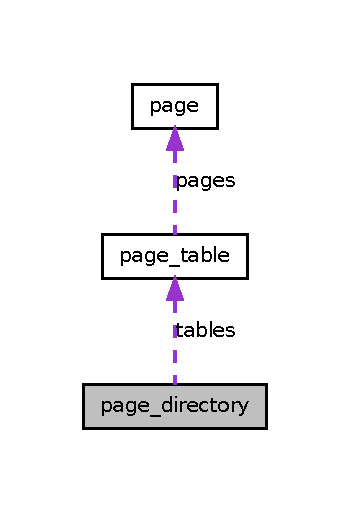
\includegraphics[width=168pt]{structpage__directory__coll__graph}
\end{center}
\end{figure}
\subsection*{Data Fields}
\begin{DoxyCompactItemize}
\item 
\hyperlink{structpage__table}{page\_\-array} $\ast$ \hyperlink{structpage__directory_a20d9b0b21070dd2f4b7fe1c8058fc238}{tables} \mbox{[}1024\mbox{]}
\item 
\hyperlink{library_8h_ad7ecf93b77285d9bf039d27fa3f1a588}{u32int} \hyperlink{structpage__directory_aaf911c2f3321b2ec2ad793b652da16fa}{physical\_\-tables} \mbox{[}1024\mbox{]}
\item 
\hyperlink{library_8h_ad7ecf93b77285d9bf039d27fa3f1a588}{u32int} \hyperlink{structpage__directory_a598f67da6db982f143737c0353f12e80}{physical\_\-address}
\end{DoxyCompactItemize}


\subsection{Field Documentation}
\hypertarget{structpage__directory_a598f67da6db982f143737c0353f12e80}{
\index{page\_\-directory@{page\_\-directory}!physical\_\-address@{physical\_\-address}}
\index{physical\_\-address@{physical\_\-address}!page_directory@{page\_\-directory}}
\subsubsection[{physical\_\-address}]{\setlength{\rightskip}{0pt plus 5cm}{\bf u32int} {\bf physical\_\-address}}}
\label{structpage__directory_a598f67da6db982f143737c0353f12e80}
\hypertarget{structpage__directory_aaf911c2f3321b2ec2ad793b652da16fa}{
\index{page\_\-directory@{page\_\-directory}!physical\_\-tables@{physical\_\-tables}}
\index{physical\_\-tables@{physical\_\-tables}!page_directory@{page\_\-directory}}
\subsubsection[{physical\_\-tables}]{\setlength{\rightskip}{0pt plus 5cm}{\bf u32int} {\bf physical\_\-tables}\mbox{[}1024\mbox{]}}}
\label{structpage__directory_aaf911c2f3321b2ec2ad793b652da16fa}
\hypertarget{structpage__directory_a20d9b0b21070dd2f4b7fe1c8058fc238}{
\index{page\_\-directory@{page\_\-directory}!tables@{tables}}
\index{tables@{tables}!page_directory@{page\_\-directory}}
\subsubsection[{tables}]{\setlength{\rightskip}{0pt plus 5cm}{\bf page\_\-array}$\ast$ {\bf tables}\mbox{[}1024\mbox{]}}}
\label{structpage__directory_a20d9b0b21070dd2f4b7fe1c8058fc238}


The documentation for this struct was generated from the following file:\begin{DoxyCompactItemize}
\item 
\hyperlink{paging_8h}{paging.h}\end{DoxyCompactItemize}

\hypertarget{structpage__table}{
\section{page\_\-table Struct Reference}
\label{structpage__table}\index{page\_\-table@{page\_\-table}}
}


{\ttfamily \#include $<$paging.h$>$}



Collaboration diagram for page\_\-table:\nopagebreak
\begin{figure}[H]
\begin{center}
\leavevmode
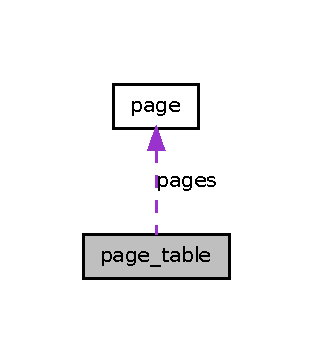
\includegraphics[width=150pt]{structpage__table__coll__graph}
\end{center}
\end{figure}
\subsection*{Data Fields}
\begin{DoxyCompactItemize}
\item 
\hyperlink{structpage}{page\_\-properties} \hyperlink{structpage__table_aaa911a7bd72c51b64df7bce29575eebe}{pages} \mbox{[}1024\mbox{]}
\end{DoxyCompactItemize}


\subsection{Field Documentation}
\hypertarget{structpage__table_aaa911a7bd72c51b64df7bce29575eebe}{
\index{page\_\-table@{page\_\-table}!pages@{pages}}
\index{pages@{pages}!page_table@{page\_\-table}}
\subsubsection[{pages}]{\setlength{\rightskip}{0pt plus 5cm}{\bf page\_\-properties} {\bf pages}\mbox{[}1024\mbox{]}}}
\label{structpage__table_aaa911a7bd72c51b64df7bce29575eebe}


The documentation for this struct was generated from the following file:\begin{DoxyCompactItemize}
\item 
\hyperlink{paging_8h}{paging.h}\end{DoxyCompactItemize}

\hypertarget{structregisters}{
\section{registers Struct Reference}
\label{structregisters}\index{registers@{registers}}
}


{\ttfamily \#include $<$isr.h$>$}

\subsection*{Data Fields}
\begin{DoxyCompactItemize}
\item 
\hyperlink{library_8h_ad7ecf93b77285d9bf039d27fa3f1a588}{u32int} \hyperlink{structregisters_a27b615cc9d414c57f335c1744908fbd1}{ds}
\item 
\hyperlink{library_8h_ad7ecf93b77285d9bf039d27fa3f1a588}{u32int} \hyperlink{structregisters_ab42cc86f60a286d9cb20116b853239ff}{edi}
\item 
\hyperlink{library_8h_ad7ecf93b77285d9bf039d27fa3f1a588}{u32int} \hyperlink{structregisters_a031d176a324992b1ef7c3b7335383590}{esi}
\item 
\hyperlink{library_8h_ad7ecf93b77285d9bf039d27fa3f1a588}{u32int} \hyperlink{structregisters_a98b65807686fee47d4061d2f2ea8578a}{ebp}
\item 
\hyperlink{library_8h_ad7ecf93b77285d9bf039d27fa3f1a588}{u32int} \hyperlink{structregisters_a7c8cdb0e23278dc958565ee9a5ebb14b}{esp}
\item 
\hyperlink{library_8h_ad7ecf93b77285d9bf039d27fa3f1a588}{u32int} \hyperlink{structregisters_aab632bcfbdfeee937cc42940432af39a}{ebx}
\item 
\hyperlink{library_8h_ad7ecf93b77285d9bf039d27fa3f1a588}{u32int} \hyperlink{structregisters_aeef91c926bff500767180c01b413a537}{edx}
\item 
\hyperlink{library_8h_ad7ecf93b77285d9bf039d27fa3f1a588}{u32int} \hyperlink{structregisters_aab67c5aaaf6afb6a2c47a4c81fb0d567}{ecx}
\item 
\hyperlink{library_8h_ad7ecf93b77285d9bf039d27fa3f1a588}{u32int} \hyperlink{structregisters_aa4608f9844ee6e6e638c487a8c8aa14f}{eax}
\item 
\hyperlink{library_8h_ad7ecf93b77285d9bf039d27fa3f1a588}{u32int} \hyperlink{structregisters_a43eb1111b811b27ece63da7c761004f2}{int\_\-no}
\item 
\hyperlink{library_8h_ad7ecf93b77285d9bf039d27fa3f1a588}{u32int} \hyperlink{structregisters_a4fd8634e5227ec539a055123d1882356}{err\_\-code}
\item 
\hyperlink{library_8h_ad7ecf93b77285d9bf039d27fa3f1a588}{u32int} \hyperlink{structregisters_ac6586230a521f5a60cded255700eaa79}{eip}
\item 
\hyperlink{library_8h_ad7ecf93b77285d9bf039d27fa3f1a588}{u32int} \hyperlink{structregisters_aff16eb39266599b77ad4025e1cf36c4e}{cs}
\item 
\hyperlink{library_8h_ad7ecf93b77285d9bf039d27fa3f1a588}{u32int} \hyperlink{structregisters_a1d2e9eee9e5db4c3658f2d72065463f3}{eflags}
\item 
\hyperlink{library_8h_ad7ecf93b77285d9bf039d27fa3f1a588}{u32int} \hyperlink{structregisters_a33d89c6cf55cb45b65ef912e9deff07e}{useresp}
\item 
\hyperlink{library_8h_ad7ecf93b77285d9bf039d27fa3f1a588}{u32int} \hyperlink{structregisters_a2d24d5fa0b7085227a24aef88db016f3}{ss}
\end{DoxyCompactItemize}


\subsection{Field Documentation}
\hypertarget{structregisters_aff16eb39266599b77ad4025e1cf36c4e}{
\index{registers@{registers}!cs@{cs}}
\index{cs@{cs}!registers@{registers}}
\subsubsection[{cs}]{\setlength{\rightskip}{0pt plus 5cm}{\bf u32int} {\bf cs}}}
\label{structregisters_aff16eb39266599b77ad4025e1cf36c4e}
\hypertarget{structregisters_a27b615cc9d414c57f335c1744908fbd1}{
\index{registers@{registers}!ds@{ds}}
\index{ds@{ds}!registers@{registers}}
\subsubsection[{ds}]{\setlength{\rightskip}{0pt plus 5cm}{\bf u32int} {\bf ds}}}
\label{structregisters_a27b615cc9d414c57f335c1744908fbd1}
\hypertarget{structregisters_aa4608f9844ee6e6e638c487a8c8aa14f}{
\index{registers@{registers}!eax@{eax}}
\index{eax@{eax}!registers@{registers}}
\subsubsection[{eax}]{\setlength{\rightskip}{0pt plus 5cm}{\bf u32int} {\bf eax}}}
\label{structregisters_aa4608f9844ee6e6e638c487a8c8aa14f}
\hypertarget{structregisters_a98b65807686fee47d4061d2f2ea8578a}{
\index{registers@{registers}!ebp@{ebp}}
\index{ebp@{ebp}!registers@{registers}}
\subsubsection[{ebp}]{\setlength{\rightskip}{0pt plus 5cm}{\bf u32int} {\bf ebp}}}
\label{structregisters_a98b65807686fee47d4061d2f2ea8578a}
\hypertarget{structregisters_aab632bcfbdfeee937cc42940432af39a}{
\index{registers@{registers}!ebx@{ebx}}
\index{ebx@{ebx}!registers@{registers}}
\subsubsection[{ebx}]{\setlength{\rightskip}{0pt plus 5cm}{\bf u32int} {\bf ebx}}}
\label{structregisters_aab632bcfbdfeee937cc42940432af39a}
\hypertarget{structregisters_aab67c5aaaf6afb6a2c47a4c81fb0d567}{
\index{registers@{registers}!ecx@{ecx}}
\index{ecx@{ecx}!registers@{registers}}
\subsubsection[{ecx}]{\setlength{\rightskip}{0pt plus 5cm}{\bf u32int} {\bf ecx}}}
\label{structregisters_aab67c5aaaf6afb6a2c47a4c81fb0d567}
\hypertarget{structregisters_ab42cc86f60a286d9cb20116b853239ff}{
\index{registers@{registers}!edi@{edi}}
\index{edi@{edi}!registers@{registers}}
\subsubsection[{edi}]{\setlength{\rightskip}{0pt plus 5cm}{\bf u32int} {\bf edi}}}
\label{structregisters_ab42cc86f60a286d9cb20116b853239ff}
\hypertarget{structregisters_aeef91c926bff500767180c01b413a537}{
\index{registers@{registers}!edx@{edx}}
\index{edx@{edx}!registers@{registers}}
\subsubsection[{edx}]{\setlength{\rightskip}{0pt plus 5cm}{\bf u32int} {\bf edx}}}
\label{structregisters_aeef91c926bff500767180c01b413a537}
\hypertarget{structregisters_a1d2e9eee9e5db4c3658f2d72065463f3}{
\index{registers@{registers}!eflags@{eflags}}
\index{eflags@{eflags}!registers@{registers}}
\subsubsection[{eflags}]{\setlength{\rightskip}{0pt plus 5cm}{\bf u32int} {\bf eflags}}}
\label{structregisters_a1d2e9eee9e5db4c3658f2d72065463f3}
\hypertarget{structregisters_ac6586230a521f5a60cded255700eaa79}{
\index{registers@{registers}!eip@{eip}}
\index{eip@{eip}!registers@{registers}}
\subsubsection[{eip}]{\setlength{\rightskip}{0pt plus 5cm}{\bf u32int} {\bf eip}}}
\label{structregisters_ac6586230a521f5a60cded255700eaa79}
\hypertarget{structregisters_a4fd8634e5227ec539a055123d1882356}{
\index{registers@{registers}!err\_\-code@{err\_\-code}}
\index{err\_\-code@{err\_\-code}!registers@{registers}}
\subsubsection[{err\_\-code}]{\setlength{\rightskip}{0pt plus 5cm}{\bf u32int} {\bf err\_\-code}}}
\label{structregisters_a4fd8634e5227ec539a055123d1882356}
\hypertarget{structregisters_a031d176a324992b1ef7c3b7335383590}{
\index{registers@{registers}!esi@{esi}}
\index{esi@{esi}!registers@{registers}}
\subsubsection[{esi}]{\setlength{\rightskip}{0pt plus 5cm}{\bf u32int} {\bf esi}}}
\label{structregisters_a031d176a324992b1ef7c3b7335383590}
\hypertarget{structregisters_a7c8cdb0e23278dc958565ee9a5ebb14b}{
\index{registers@{registers}!esp@{esp}}
\index{esp@{esp}!registers@{registers}}
\subsubsection[{esp}]{\setlength{\rightskip}{0pt plus 5cm}{\bf u32int} {\bf esp}}}
\label{structregisters_a7c8cdb0e23278dc958565ee9a5ebb14b}
\hypertarget{structregisters_a43eb1111b811b27ece63da7c761004f2}{
\index{registers@{registers}!int\_\-no@{int\_\-no}}
\index{int\_\-no@{int\_\-no}!registers@{registers}}
\subsubsection[{int\_\-no}]{\setlength{\rightskip}{0pt plus 5cm}{\bf u32int} {\bf int\_\-no}}}
\label{structregisters_a43eb1111b811b27ece63da7c761004f2}
\hypertarget{structregisters_a2d24d5fa0b7085227a24aef88db016f3}{
\index{registers@{registers}!ss@{ss}}
\index{ss@{ss}!registers@{registers}}
\subsubsection[{ss}]{\setlength{\rightskip}{0pt plus 5cm}{\bf u32int} {\bf ss}}}
\label{structregisters_a2d24d5fa0b7085227a24aef88db016f3}
\hypertarget{structregisters_a33d89c6cf55cb45b65ef912e9deff07e}{
\index{registers@{registers}!useresp@{useresp}}
\index{useresp@{useresp}!registers@{registers}}
\subsubsection[{useresp}]{\setlength{\rightskip}{0pt plus 5cm}{\bf u32int} {\bf useresp}}}
\label{structregisters_a33d89c6cf55cb45b65ef912e9deff07e}


The documentation for this struct was generated from the following file:\begin{DoxyCompactItemize}
\item 
\hyperlink{isr_8h}{isr.h}\end{DoxyCompactItemize}

\hypertarget{structthread__node}{
\section{thread\_\-node Struct Reference}
\label{structthread__node}\index{thread\_\-node@{thread\_\-node}}
}


{\ttfamily \#include $<$task\_\-scheduler.h$>$}



Collaboration diagram for thread\_\-node:\nopagebreak
\begin{figure}[H]
\begin{center}
\leavevmode
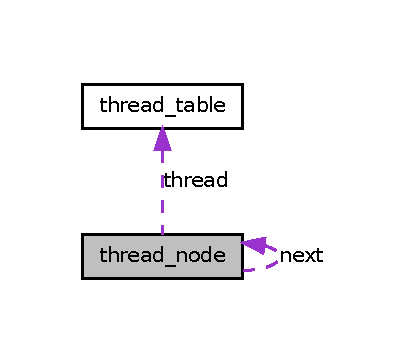
\includegraphics[width=196pt]{structthread__node__coll__graph}
\end{center}
\end{figure}
\subsection*{Data Fields}
\begin{DoxyCompactItemize}
\item 
\hyperlink{structthread__table}{thread\_\-table} $\ast$ \hyperlink{structthread__node_ae52e1333aac15af28b6c73736a95c1b2}{thread}
\item 
struct \hyperlink{structthread__node}{thread\_\-node} $\ast$ \hyperlink{structthread__node_a051ce7e25364ca47a00f5f1bc1e3eaf5}{next}
\end{DoxyCompactItemize}


\subsection{Field Documentation}
\hypertarget{structthread__node_a051ce7e25364ca47a00f5f1bc1e3eaf5}{
\index{thread\_\-node@{thread\_\-node}!next@{next}}
\index{next@{next}!thread_node@{thread\_\-node}}
\subsubsection[{next}]{\setlength{\rightskip}{0pt plus 5cm}struct {\bf thread\_\-node}$\ast$ {\bf next}}}
\label{structthread__node_a051ce7e25364ca47a00f5f1bc1e3eaf5}
\hypertarget{structthread__node_ae52e1333aac15af28b6c73736a95c1b2}{
\index{thread\_\-node@{thread\_\-node}!thread@{thread}}
\index{thread@{thread}!thread_node@{thread\_\-node}}
\subsubsection[{thread}]{\setlength{\rightskip}{0pt plus 5cm}{\bf thread\_\-table}$\ast$ {\bf thread}}}
\label{structthread__node_ae52e1333aac15af28b6c73736a95c1b2}


The documentation for this struct was generated from the following file:\begin{DoxyCompactItemize}
\item 
\hyperlink{task__scheduler_8h}{task\_\-scheduler.h}\end{DoxyCompactItemize}

\hypertarget{structthread__table}{
\section{thread\_\-table Struct Reference}
\label{structthread__table}\index{thread\_\-table@{thread\_\-table}}
}


{\ttfamily \#include $<$thread.h$>$}

\subsection*{Data Fields}
\begin{DoxyCompactItemize}
\item 
\hyperlink{library_8h_ad7ecf93b77285d9bf039d27fa3f1a588}{u32int} \hyperlink{structthread__table_a5b065679595c5c6c708349d563e35b6c}{id}
\item 
\hyperlink{library_8h_ad7ecf93b77285d9bf039d27fa3f1a588}{u32int} \hyperlink{structthread__table_a7c8cdb0e23278dc958565ee9a5ebb14b}{esp}
\item 
\hyperlink{library_8h_ad7ecf93b77285d9bf039d27fa3f1a588}{u32int} \hyperlink{structthread__table_a98b65807686fee47d4061d2f2ea8578a}{ebp}
\item 
\hyperlink{library_8h_ad7ecf93b77285d9bf039d27fa3f1a588}{u32int} \hyperlink{structthread__table_aab632bcfbdfeee937cc42940432af39a}{ebx}
\item 
\hyperlink{library_8h_ad7ecf93b77285d9bf039d27fa3f1a588}{u32int} \hyperlink{structthread__table_a031d176a324992b1ef7c3b7335383590}{esi}
\item 
\hyperlink{library_8h_ad7ecf93b77285d9bf039d27fa3f1a588}{u32int} \hyperlink{structthread__table_ab42cc86f60a286d9cb20116b853239ff}{edi}
\end{DoxyCompactItemize}


\subsection{Field Documentation}
\hypertarget{structthread__table_a98b65807686fee47d4061d2f2ea8578a}{
\index{thread\_\-table@{thread\_\-table}!ebp@{ebp}}
\index{ebp@{ebp}!thread_table@{thread\_\-table}}
\subsubsection[{ebp}]{\setlength{\rightskip}{0pt plus 5cm}{\bf u32int} {\bf ebp}}}
\label{structthread__table_a98b65807686fee47d4061d2f2ea8578a}
\hypertarget{structthread__table_aab632bcfbdfeee937cc42940432af39a}{
\index{thread\_\-table@{thread\_\-table}!ebx@{ebx}}
\index{ebx@{ebx}!thread_table@{thread\_\-table}}
\subsubsection[{ebx}]{\setlength{\rightskip}{0pt plus 5cm}{\bf u32int} {\bf ebx}}}
\label{structthread__table_aab632bcfbdfeee937cc42940432af39a}
\hypertarget{structthread__table_ab42cc86f60a286d9cb20116b853239ff}{
\index{thread\_\-table@{thread\_\-table}!edi@{edi}}
\index{edi@{edi}!thread_table@{thread\_\-table}}
\subsubsection[{edi}]{\setlength{\rightskip}{0pt plus 5cm}{\bf u32int} {\bf edi}}}
\label{structthread__table_ab42cc86f60a286d9cb20116b853239ff}
\hypertarget{structthread__table_a031d176a324992b1ef7c3b7335383590}{
\index{thread\_\-table@{thread\_\-table}!esi@{esi}}
\index{esi@{esi}!thread_table@{thread\_\-table}}
\subsubsection[{esi}]{\setlength{\rightskip}{0pt plus 5cm}{\bf u32int} {\bf esi}}}
\label{structthread__table_a031d176a324992b1ef7c3b7335383590}
\hypertarget{structthread__table_a7c8cdb0e23278dc958565ee9a5ebb14b}{
\index{thread\_\-table@{thread\_\-table}!esp@{esp}}
\index{esp@{esp}!thread_table@{thread\_\-table}}
\subsubsection[{esp}]{\setlength{\rightskip}{0pt plus 5cm}{\bf u32int} {\bf esp}}}
\label{structthread__table_a7c8cdb0e23278dc958565ee9a5ebb14b}
\hypertarget{structthread__table_a5b065679595c5c6c708349d563e35b6c}{
\index{thread\_\-table@{thread\_\-table}!id@{id}}
\index{id@{id}!thread_table@{thread\_\-table}}
\subsubsection[{id}]{\setlength{\rightskip}{0pt plus 5cm}{\bf u32int} {\bf id}}}
\label{structthread__table_a5b065679595c5c6c708349d563e35b6c}


The documentation for this struct was generated from the following file:\begin{DoxyCompactItemize}
\item 
\hyperlink{thread_8h}{thread.h}\end{DoxyCompactItemize}

\chapter{File Documentation}
\hypertarget{descriptor__tables_8c}{
\section{descriptor\_\-tables.c File Reference}
\label{descriptor__tables_8c}\index{descriptor\_\-tables.c@{descriptor\_\-tables.c}}
}
{\ttfamily \#include \char`\"{}library.h\char`\"{}}\par
{\ttfamily \#include \char`\"{}descriptor\_\-tables.h\char`\"{}}\par
{\ttfamily \#include \char`\"{}isr.h\char`\"{}}\par
Include dependency graph for descriptor\_\-tables.c:
\nopagebreak
\begin{figure}[H]
\begin{center}
\leavevmode
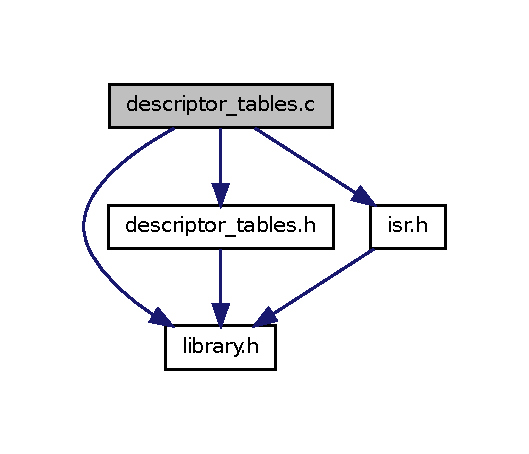
\includegraphics[width=254pt]{descriptor__tables_8c__incl}
\end{center}
\end{figure}
\subsection*{Functions}
\begin{DoxyCompactItemize}
\item 
void \hyperlink{descriptor__tables_8c_af3833dc9063c90b6758a50b1101f54b1}{gdt\_\-flush} (\hyperlink{library_8h_ad7ecf93b77285d9bf039d27fa3f1a588}{u32int})
\item 
void \hyperlink{descriptor__tables_8c_a7f063f0c0d27643faa13723e8086b808}{idt\_\-flush} (\hyperlink{library_8h_ad7ecf93b77285d9bf039d27fa3f1a588}{u32int})
\item 
void \hyperlink{descriptor__tables_8c_a29b68b6342c3a52a54ad89ec23945472}{init\_\-descriptor\_\-tables} ()
\end{DoxyCompactItemize}
\subsection*{Variables}
\begin{DoxyCompactItemize}
\item 
\hyperlink{structgdt__entry}{gdt\_\-table} \hyperlink{descriptor__tables_8c_a00efdd13934ce42461d7e4417b2eda92}{gdt} \mbox{[}5\mbox{]}
\item 
\hyperlink{structgdt__ptr}{gdt\_\-pointer} \hyperlink{descriptor__tables_8c_a26e247caad4c6048482c5327b6d9ec47}{gp}
\item 
\hyperlink{structidt__entry__struct}{idt\_\-entry\_\-t} \hyperlink{descriptor__tables_8c_a02c62ffc54da283f5faaa40b125d2dce}{idt\_\-entries} \mbox{[}256\mbox{]}
\item 
\hyperlink{structidt__ptr__struct}{idt\_\-ptr\_\-t} \hyperlink{descriptor__tables_8c_a3f2660783240a0a506d85e3750dff814}{idt\_\-ptr}
\item 
\hyperlink{isr_8h_acf628c2f58c1c719fd6f9c879ab5ddf4}{isr\_\-t} \hyperlink{descriptor__tables_8c_a3bec2371c4d67ab6e9e76cd48cd2d9fb}{interrupt\_\-handlers} \mbox{[}$\,$\mbox{]}
\end{DoxyCompactItemize}


\subsection{Function Documentation}
\hypertarget{descriptor__tables_8c_af3833dc9063c90b6758a50b1101f54b1}{
\index{descriptor\_\-tables.c@{descriptor\_\-tables.c}!gdt\_\-flush@{gdt\_\-flush}}
\index{gdt\_\-flush@{gdt\_\-flush}!descriptor_tables.c@{descriptor\_\-tables.c}}
\subsubsection[{gdt\_\-flush}]{\setlength{\rightskip}{0pt plus 5cm}void gdt\_\-flush (
\begin{DoxyParamCaption}
\item[{{\bf u32int}}]{}
\end{DoxyParamCaption}
)}}
\label{descriptor__tables_8c_af3833dc9063c90b6758a50b1101f54b1}
\hypertarget{descriptor__tables_8c_a7f063f0c0d27643faa13723e8086b808}{
\index{descriptor\_\-tables.c@{descriptor\_\-tables.c}!idt\_\-flush@{idt\_\-flush}}
\index{idt\_\-flush@{idt\_\-flush}!descriptor_tables.c@{descriptor\_\-tables.c}}
\subsubsection[{idt\_\-flush}]{\setlength{\rightskip}{0pt plus 5cm}void idt\_\-flush (
\begin{DoxyParamCaption}
\item[{{\bf u32int}}]{}
\end{DoxyParamCaption}
)}}
\label{descriptor__tables_8c_a7f063f0c0d27643faa13723e8086b808}
\hypertarget{descriptor__tables_8c_a29b68b6342c3a52a54ad89ec23945472}{
\index{descriptor\_\-tables.c@{descriptor\_\-tables.c}!init\_\-descriptor\_\-tables@{init\_\-descriptor\_\-tables}}
\index{init\_\-descriptor\_\-tables@{init\_\-descriptor\_\-tables}!descriptor_tables.c@{descriptor\_\-tables.c}}
\subsubsection[{init\_\-descriptor\_\-tables}]{\setlength{\rightskip}{0pt plus 5cm}void init\_\-descriptor\_\-tables (
\begin{DoxyParamCaption}
{}
\end{DoxyParamCaption}
)}}
\label{descriptor__tables_8c_a29b68b6342c3a52a54ad89ec23945472}


Here is the call graph for this function:
\nopagebreak
\begin{figure}[H]
\begin{center}
\leavevmode
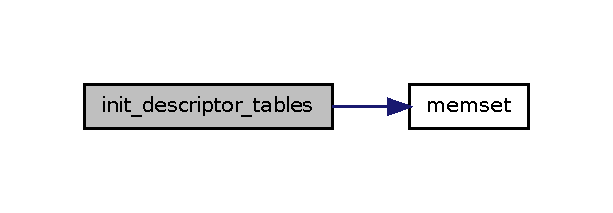
\includegraphics[width=294pt]{descriptor__tables_8c_a29b68b6342c3a52a54ad89ec23945472_cgraph}
\end{center}
\end{figure}




Here is the caller graph for this function:
\nopagebreak
\begin{figure}[H]
\begin{center}
\leavevmode
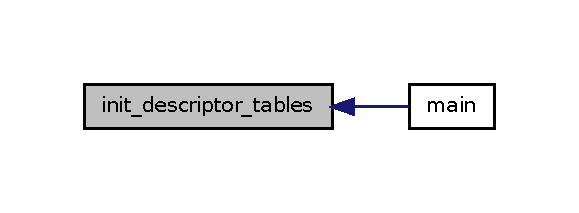
\includegraphics[width=278pt]{descriptor__tables_8c_a29b68b6342c3a52a54ad89ec23945472_icgraph}
\end{center}
\end{figure}




\subsection{Variable Documentation}
\hypertarget{descriptor__tables_8c_a00efdd13934ce42461d7e4417b2eda92}{
\index{descriptor\_\-tables.c@{descriptor\_\-tables.c}!gdt@{gdt}}
\index{gdt@{gdt}!descriptor_tables.c@{descriptor\_\-tables.c}}
\subsubsection[{gdt}]{\setlength{\rightskip}{0pt plus 5cm}{\bf gdt\_\-table} {\bf gdt}\mbox{[}5\mbox{]}}}
\label{descriptor__tables_8c_a00efdd13934ce42461d7e4417b2eda92}
\hypertarget{descriptor__tables_8c_a26e247caad4c6048482c5327b6d9ec47}{
\index{descriptor\_\-tables.c@{descriptor\_\-tables.c}!gp@{gp}}
\index{gp@{gp}!descriptor_tables.c@{descriptor\_\-tables.c}}
\subsubsection[{gp}]{\setlength{\rightskip}{0pt plus 5cm}{\bf gdt\_\-pointer} {\bf gp}}}
\label{descriptor__tables_8c_a26e247caad4c6048482c5327b6d9ec47}
\hypertarget{descriptor__tables_8c_a02c62ffc54da283f5faaa40b125d2dce}{
\index{descriptor\_\-tables.c@{descriptor\_\-tables.c}!idt\_\-entries@{idt\_\-entries}}
\index{idt\_\-entries@{idt\_\-entries}!descriptor_tables.c@{descriptor\_\-tables.c}}
\subsubsection[{idt\_\-entries}]{\setlength{\rightskip}{0pt plus 5cm}{\bf idt\_\-entry\_\-t} {\bf idt\_\-entries}\mbox{[}256\mbox{]}}}
\label{descriptor__tables_8c_a02c62ffc54da283f5faaa40b125d2dce}
\hypertarget{descriptor__tables_8c_a3f2660783240a0a506d85e3750dff814}{
\index{descriptor\_\-tables.c@{descriptor\_\-tables.c}!idt\_\-ptr@{idt\_\-ptr}}
\index{idt\_\-ptr@{idt\_\-ptr}!descriptor_tables.c@{descriptor\_\-tables.c}}
\subsubsection[{idt\_\-ptr}]{\setlength{\rightskip}{0pt plus 5cm}{\bf idt\_\-ptr\_\-t} {\bf idt\_\-ptr}}}
\label{descriptor__tables_8c_a3f2660783240a0a506d85e3750dff814}
\hypertarget{descriptor__tables_8c_a3bec2371c4d67ab6e9e76cd48cd2d9fb}{
\index{descriptor\_\-tables.c@{descriptor\_\-tables.c}!interrupt\_\-handlers@{interrupt\_\-handlers}}
\index{interrupt\_\-handlers@{interrupt\_\-handlers}!descriptor_tables.c@{descriptor\_\-tables.c}}
\subsubsection[{interrupt\_\-handlers}]{\setlength{\rightskip}{0pt plus 5cm}{\bf isr\_\-t} {\bf interrupt\_\-handlers}\mbox{[}$\,$\mbox{]}}}
\label{descriptor__tables_8c_a3bec2371c4d67ab6e9e76cd48cd2d9fb}

\hypertarget{descriptor__tables_8h}{
\section{descriptor\_\-tables.h File Reference}
\label{descriptor__tables_8h}\index{descriptor\_\-tables.h@{descriptor\_\-tables.h}}
}
{\ttfamily \#include \char`\"{}library.h\char`\"{}}\par
Include dependency graph for descriptor\_\-tables.h:
\nopagebreak
\begin{figure}[H]
\begin{center}
\leavevmode
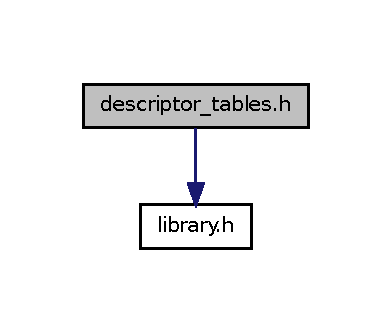
\includegraphics[width=188pt]{descriptor__tables_8h__incl}
\end{center}
\end{figure}
This graph shows which files directly or indirectly include this file:
\nopagebreak
\begin{figure}[H]
\begin{center}
\leavevmode
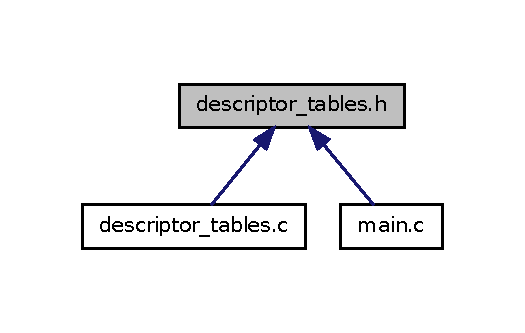
\includegraphics[width=252pt]{descriptor__tables_8h__dep__incl}
\end{center}
\end{figure}
\subsection*{Data Structures}
\begin{DoxyCompactItemize}
\item 
struct \hyperlink{structgdt__entry}{gdt\_\-entry}
\item 
struct \hyperlink{structgdt__ptr}{gdt\_\-ptr}
\item 
struct \hyperlink{structidt__entry__struct}{idt\_\-entry\_\-struct}
\item 
struct \hyperlink{structidt__ptr__struct}{idt\_\-ptr\_\-struct}
\end{DoxyCompactItemize}
\subsection*{Typedefs}
\begin{DoxyCompactItemize}
\item 
typedef struct \hyperlink{structgdt__entry}{gdt\_\-entry} \hyperlink{descriptor__tables_8h_ae6bb1d5e1813d91b59c37f22badc643c}{gdt\_\-table}
\item 
typedef struct \hyperlink{structgdt__ptr}{gdt\_\-ptr} \hyperlink{descriptor__tables_8h_a1a633700efa4a9f0cc87f8d1e591502f}{gdt\_\-pointer}
\item 
typedef struct \hyperlink{structidt__entry__struct}{idt\_\-entry\_\-struct} \hyperlink{descriptor__tables_8h_a1ad45e5b006481ff3604f7b54bd26e13}{idt\_\-entry\_\-t}
\item 
typedef struct \hyperlink{structidt__ptr__struct}{idt\_\-ptr\_\-struct} \hyperlink{descriptor__tables_8h_a4c173f183e148c7a8a8c1ed9214b909e}{idt\_\-ptr\_\-t}
\end{DoxyCompactItemize}
\subsection*{Functions}
\begin{DoxyCompactItemize}
\item 
void \hyperlink{descriptor__tables_8h_a29b68b6342c3a52a54ad89ec23945472}{init\_\-descriptor\_\-tables} ()
\item 
struct \hyperlink{structgdt__entry}{gdt\_\-entry} \hyperlink{descriptor__tables_8h_ae21df847b32e33e64ba0912dd628e610}{\_\-\_\-attribute\_\-\_\-} ((packed))
\item 
void \hyperlink{descriptor__tables_8h_af88eb8e98d943aa0461c01de3cb53493}{isr0} ()
\item 
void \hyperlink{descriptor__tables_8h_aeab0ed9ae661801c25f7dc9089c19f72}{isr1} ()
\item 
void \hyperlink{descriptor__tables_8h_a99e457875cca040c3f7c77b61e960b53}{isr2} ()
\item 
void \hyperlink{descriptor__tables_8h_a0ef268d2c16a7b318356451a05fd507b}{isr3} ()
\item 
void \hyperlink{descriptor__tables_8h_a09af768d636144aaeaddd76c92a0a2f5}{isr4} ()
\item 
void \hyperlink{descriptor__tables_8h_aa91d821a4bcafb44933d92945727b0df}{isr5} ()
\item 
void \hyperlink{descriptor__tables_8h_a9fadb95f34937b1ded02c4171b4920ba}{isr6} ()
\item 
void \hyperlink{descriptor__tables_8h_a7eb6ec30db7077fb1c9c9d926a0fc407}{isr7} ()
\item 
void \hyperlink{descriptor__tables_8h_a86bc69345a3bb409665dbadb77a9d393}{isr8} ()
\item 
void \hyperlink{descriptor__tables_8h_aacb7c8490cbd623a3a2bf933ffedd131}{isr9} ()
\item 
void \hyperlink{descriptor__tables_8h_a3c8cb1341cf756883a2e7dc317d5272d}{isr10} ()
\item 
void \hyperlink{descriptor__tables_8h_a0d8145cf6ee1ef7834f459ba777d323c}{isr11} ()
\item 
void \hyperlink{descriptor__tables_8h_a00f00421039cb85f9dd9375995c784bd}{isr12} ()
\item 
void \hyperlink{descriptor__tables_8h_af985dcf66872ee696e5f30d819ac16a1}{isr13} ()
\item 
void \hyperlink{descriptor__tables_8h_a8b63eaa37c03743718870964a3429ba8}{isr14} ()
\item 
void \hyperlink{descriptor__tables_8h_a9160f355325318a990c106ad5c3b8954}{isr15} ()
\item 
void \hyperlink{descriptor__tables_8h_add0980c10028b377643da169e52e5be7}{isr16} ()
\item 
void \hyperlink{descriptor__tables_8h_ac7d1e81e585bc7c56b46280006402f9e}{isr17} ()
\item 
void \hyperlink{descriptor__tables_8h_ae685c5ca5ed9c9c5e7d297ad8d14de49}{isr18} ()
\item 
void \hyperlink{descriptor__tables_8h_ad16b5f77287df551e63d3f0c67f8f75d}{isr19} ()
\item 
void \hyperlink{descriptor__tables_8h_a552d2aedae97d97083d3f9caf6ad59a5}{isr20} ()
\item 
void \hyperlink{descriptor__tables_8h_af106b9a26e06abf17eebb6f7ae54f905}{isr21} ()
\item 
void \hyperlink{descriptor__tables_8h_aa4b6f47f27ac3b31fc426f5c2a1a669c}{isr22} ()
\item 
void \hyperlink{descriptor__tables_8h_a277e9cc418a637ae584c1ff6525eb2e1}{isr23} ()
\item 
void \hyperlink{descriptor__tables_8h_a2ea113ad8536ca8311ab00d077ece7f1}{isr24} ()
\item 
void \hyperlink{descriptor__tables_8h_a73e919f327e846f72b99de088ae9b822}{isr25} ()
\item 
void \hyperlink{descriptor__tables_8h_a24c118fd7e75c96d19da1bbaf87731e4}{isr26} ()
\item 
void \hyperlink{descriptor__tables_8h_ad97e98084cbcdc21bf03ba314dc243e0}{isr27} ()
\item 
void \hyperlink{descriptor__tables_8h_ab2a5fe4d3cf67be0c67db612aa757c5f}{isr28} ()
\item 
void \hyperlink{descriptor__tables_8h_a8cce4d55d6a199607cd3a9e2a33241b2}{isr29} ()
\item 
void \hyperlink{descriptor__tables_8h_af868664393aedd51c04e3ddd48b8f84f}{isr30} ()
\item 
void \hyperlink{descriptor__tables_8h_af4ae10cea59f9bb2f79c13b8036d81f1}{isr31} ()
\item 
void \hyperlink{descriptor__tables_8h_adbe0f253d11eeb032b3612c8732fb76e}{irq0} ()
\item 
void \hyperlink{descriptor__tables_8h_ab67ffa95ff39e0b264f4534d43025c30}{irq1} ()
\item 
void \hyperlink{descriptor__tables_8h_a118ba521aa61c5f0785580408a5b95cc}{irq2} ()
\item 
void \hyperlink{descriptor__tables_8h_a672afd3d2d2c7a896068f1ee94b6ac4b}{irq3} ()
\item 
void \hyperlink{descriptor__tables_8h_a6ece1319726003baeb064fa32a5e27b6}{irq4} ()
\item 
void \hyperlink{descriptor__tables_8h_a0c86295415896333de5803b5255cc3fd}{irq5} ()
\item 
void \hyperlink{descriptor__tables_8h_a4dd0a509c8829cd9d3606da7ba7cde7a}{irq6} ()
\item 
void \hyperlink{descriptor__tables_8h_aa3079d2a2ea8fdd0d36f26fb2f61e316}{irq7} ()
\item 
void \hyperlink{descriptor__tables_8h_a763933e69e7a6f5ac0d2802a56b6401b}{irq8} ()
\item 
void \hyperlink{descriptor__tables_8h_a59dbef11d3615eb79b6a13c82b5bf476}{irq9} ()
\item 
void \hyperlink{descriptor__tables_8h_a93037dcfb63ee486f11dd927f37b57af}{irq10} ()
\item 
void \hyperlink{descriptor__tables_8h_a16bf2a49a4c9a48e65c1379d91b79235}{irq11} ()
\item 
void \hyperlink{descriptor__tables_8h_a47e842053a77f6409bbd6a50cec87b5e}{irq12} ()
\item 
void \hyperlink{descriptor__tables_8h_aaf8a8dc035d379d8173b06a2ebd881a1}{irq13} ()
\item 
void \hyperlink{descriptor__tables_8h_aa63550aa0e55da846a219a2828007529}{irq14} ()
\item 
void \hyperlink{descriptor__tables_8h_a516b16b006f8c0555c15a793220e28a2}{irq15} ()
\end{DoxyCompactItemize}
\subsection*{Variables}
\begin{DoxyCompactItemize}
\item 
unsigned short \hyperlink{descriptor__tables_8h_aacba9616b9bdd5895e8dcf5567e4170c}{limit\_\-low}
\item 
unsigned short \hyperlink{descriptor__tables_8h_ae4b82d5bd06e0cad3df76bcabedfe194}{base\_\-low}
\item 
unsigned char \hyperlink{descriptor__tables_8h_a11134ae8e899bd8f22b3d59dd5b86fae}{base\_\-middle}
\item 
unsigned char \hyperlink{descriptor__tables_8h_a1466f288c685860255d8e68192262c44}{access}
\item 
unsigned char \hyperlink{descriptor__tables_8h_a97775c42d71e8858948fa91b472876fb}{granularity}
\item 
unsigned char \hyperlink{descriptor__tables_8h_a2ece4ce625dcee29c9a9e6952055ddd5}{base\_\-high}
\item 
unsigned short \hyperlink{descriptor__tables_8h_a68fd3b4f6c14a331ca9b226cbf122e13}{limit}
\item 
unsigned int \hyperlink{descriptor__tables_8h_ab5763c2b18c825c8b8fba44b2e60ddc1}{base}
\item 
\hyperlink{library_8h_a863d9497073aad2b991aeab2211d87af}{u16int} \hyperlink{descriptor__tables_8h_a87eb3dc5d98a750439e08c9e6703778b}{base\_\-lo}
\item 
\hyperlink{library_8h_a863d9497073aad2b991aeab2211d87af}{u16int} \hyperlink{descriptor__tables_8h_adf6a7546c6355a8f87f34731860b49e1}{sel}
\item 
\hyperlink{library_8h_a1026e682ffdadc1701c42cd44ce9efcf}{u8int} \hyperlink{descriptor__tables_8h_a9d3c870e7b1697c835095c536ac5b09b}{always0}
\item 
\hyperlink{library_8h_a1026e682ffdadc1701c42cd44ce9efcf}{u8int} \hyperlink{descriptor__tables_8h_a138dda98fcd4738346af61bcca8cf4b4}{flags}
\item 
\hyperlink{library_8h_a863d9497073aad2b991aeab2211d87af}{u16int} \hyperlink{descriptor__tables_8h_a65b35eebe0d81928a3ac5ddb1efe0fc3}{base\_\-hi}
\end{DoxyCompactItemize}


\subsection{Typedef Documentation}
\hypertarget{descriptor__tables_8h_a1a633700efa4a9f0cc87f8d1e591502f}{
\index{descriptor\_\-tables.h@{descriptor\_\-tables.h}!gdt\_\-pointer@{gdt\_\-pointer}}
\index{gdt\_\-pointer@{gdt\_\-pointer}!descriptor_tables.h@{descriptor\_\-tables.h}}
\subsubsection[{gdt\_\-pointer}]{\setlength{\rightskip}{0pt plus 5cm}typedef struct {\bf gdt\_\-ptr} {\bf gdt\_\-pointer}}}
\label{descriptor__tables_8h_a1a633700efa4a9f0cc87f8d1e591502f}
\hypertarget{descriptor__tables_8h_ae6bb1d5e1813d91b59c37f22badc643c}{
\index{descriptor\_\-tables.h@{descriptor\_\-tables.h}!gdt\_\-table@{gdt\_\-table}}
\index{gdt\_\-table@{gdt\_\-table}!descriptor_tables.h@{descriptor\_\-tables.h}}
\subsubsection[{gdt\_\-table}]{\setlength{\rightskip}{0pt plus 5cm}typedef struct {\bf gdt\_\-entry} {\bf gdt\_\-table}}}
\label{descriptor__tables_8h_ae6bb1d5e1813d91b59c37f22badc643c}
\hypertarget{descriptor__tables_8h_a1ad45e5b006481ff3604f7b54bd26e13}{
\index{descriptor\_\-tables.h@{descriptor\_\-tables.h}!idt\_\-entry\_\-t@{idt\_\-entry\_\-t}}
\index{idt\_\-entry\_\-t@{idt\_\-entry\_\-t}!descriptor_tables.h@{descriptor\_\-tables.h}}
\subsubsection[{idt\_\-entry\_\-t}]{\setlength{\rightskip}{0pt plus 5cm}typedef struct {\bf idt\_\-entry\_\-struct} {\bf idt\_\-entry\_\-t}}}
\label{descriptor__tables_8h_a1ad45e5b006481ff3604f7b54bd26e13}
\hypertarget{descriptor__tables_8h_a4c173f183e148c7a8a8c1ed9214b909e}{
\index{descriptor\_\-tables.h@{descriptor\_\-tables.h}!idt\_\-ptr\_\-t@{idt\_\-ptr\_\-t}}
\index{idt\_\-ptr\_\-t@{idt\_\-ptr\_\-t}!descriptor_tables.h@{descriptor\_\-tables.h}}
\subsubsection[{idt\_\-ptr\_\-t}]{\setlength{\rightskip}{0pt plus 5cm}typedef struct {\bf idt\_\-ptr\_\-struct} {\bf idt\_\-ptr\_\-t}}}
\label{descriptor__tables_8h_a4c173f183e148c7a8a8c1ed9214b909e}


\subsection{Function Documentation}
\hypertarget{descriptor__tables_8h_ae21df847b32e33e64ba0912dd628e610}{
\index{descriptor\_\-tables.h@{descriptor\_\-tables.h}!\_\-\_\-attribute\_\-\_\-@{\_\-\_\-attribute\_\-\_\-}}
\index{\_\-\_\-attribute\_\-\_\-@{\_\-\_\-attribute\_\-\_\-}!descriptor_tables.h@{descriptor\_\-tables.h}}
\subsubsection[{\_\-\_\-attribute\_\-\_\-}]{\setlength{\rightskip}{0pt plus 5cm}struct {\bf gdt\_\-entry} \_\-\_\-attribute\_\-\_\- (
\begin{DoxyParamCaption}
\item[{(packed)}]{}
\end{DoxyParamCaption}
)}}
\label{descriptor__tables_8h_ae21df847b32e33e64ba0912dd628e610}
\hypertarget{descriptor__tables_8h_a29b68b6342c3a52a54ad89ec23945472}{
\index{descriptor\_\-tables.h@{descriptor\_\-tables.h}!init\_\-descriptor\_\-tables@{init\_\-descriptor\_\-tables}}
\index{init\_\-descriptor\_\-tables@{init\_\-descriptor\_\-tables}!descriptor_tables.h@{descriptor\_\-tables.h}}
\subsubsection[{init\_\-descriptor\_\-tables}]{\setlength{\rightskip}{0pt plus 5cm}void init\_\-descriptor\_\-tables (
\begin{DoxyParamCaption}
{}
\end{DoxyParamCaption}
)}}
\label{descriptor__tables_8h_a29b68b6342c3a52a54ad89ec23945472}


Here is the call graph for this function:
\nopagebreak
\begin{figure}[H]
\begin{center}
\leavevmode
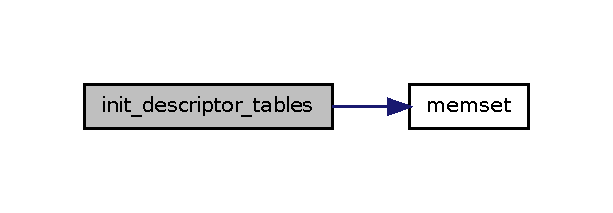
\includegraphics[width=294pt]{descriptor__tables_8h_a29b68b6342c3a52a54ad89ec23945472_cgraph}
\end{center}
\end{figure}




Here is the caller graph for this function:
\nopagebreak
\begin{figure}[H]
\begin{center}
\leavevmode
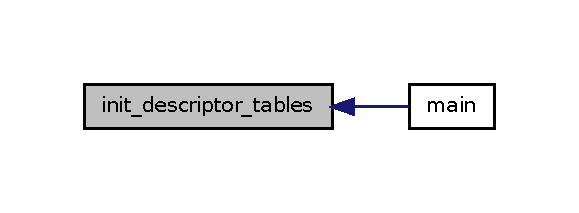
\includegraphics[width=278pt]{descriptor__tables_8h_a29b68b6342c3a52a54ad89ec23945472_icgraph}
\end{center}
\end{figure}


\hypertarget{descriptor__tables_8h_adbe0f253d11eeb032b3612c8732fb76e}{
\index{descriptor\_\-tables.h@{descriptor\_\-tables.h}!irq0@{irq0}}
\index{irq0@{irq0}!descriptor_tables.h@{descriptor\_\-tables.h}}
\subsubsection[{irq0}]{\setlength{\rightskip}{0pt plus 5cm}void irq0 (
\begin{DoxyParamCaption}
{}
\end{DoxyParamCaption}
)}}
\label{descriptor__tables_8h_adbe0f253d11eeb032b3612c8732fb76e}
\hypertarget{descriptor__tables_8h_ab67ffa95ff39e0b264f4534d43025c30}{
\index{descriptor\_\-tables.h@{descriptor\_\-tables.h}!irq1@{irq1}}
\index{irq1@{irq1}!descriptor_tables.h@{descriptor\_\-tables.h}}
\subsubsection[{irq1}]{\setlength{\rightskip}{0pt plus 5cm}void irq1 (
\begin{DoxyParamCaption}
{}
\end{DoxyParamCaption}
)}}
\label{descriptor__tables_8h_ab67ffa95ff39e0b264f4534d43025c30}
\hypertarget{descriptor__tables_8h_a93037dcfb63ee486f11dd927f37b57af}{
\index{descriptor\_\-tables.h@{descriptor\_\-tables.h}!irq10@{irq10}}
\index{irq10@{irq10}!descriptor_tables.h@{descriptor\_\-tables.h}}
\subsubsection[{irq10}]{\setlength{\rightskip}{0pt plus 5cm}void irq10 (
\begin{DoxyParamCaption}
{}
\end{DoxyParamCaption}
)}}
\label{descriptor__tables_8h_a93037dcfb63ee486f11dd927f37b57af}
\hypertarget{descriptor__tables_8h_a16bf2a49a4c9a48e65c1379d91b79235}{
\index{descriptor\_\-tables.h@{descriptor\_\-tables.h}!irq11@{irq11}}
\index{irq11@{irq11}!descriptor_tables.h@{descriptor\_\-tables.h}}
\subsubsection[{irq11}]{\setlength{\rightskip}{0pt plus 5cm}void irq11 (
\begin{DoxyParamCaption}
{}
\end{DoxyParamCaption}
)}}
\label{descriptor__tables_8h_a16bf2a49a4c9a48e65c1379d91b79235}
\hypertarget{descriptor__tables_8h_a47e842053a77f6409bbd6a50cec87b5e}{
\index{descriptor\_\-tables.h@{descriptor\_\-tables.h}!irq12@{irq12}}
\index{irq12@{irq12}!descriptor_tables.h@{descriptor\_\-tables.h}}
\subsubsection[{irq12}]{\setlength{\rightskip}{0pt plus 5cm}void irq12 (
\begin{DoxyParamCaption}
{}
\end{DoxyParamCaption}
)}}
\label{descriptor__tables_8h_a47e842053a77f6409bbd6a50cec87b5e}
\hypertarget{descriptor__tables_8h_aaf8a8dc035d379d8173b06a2ebd881a1}{
\index{descriptor\_\-tables.h@{descriptor\_\-tables.h}!irq13@{irq13}}
\index{irq13@{irq13}!descriptor_tables.h@{descriptor\_\-tables.h}}
\subsubsection[{irq13}]{\setlength{\rightskip}{0pt plus 5cm}void irq13 (
\begin{DoxyParamCaption}
{}
\end{DoxyParamCaption}
)}}
\label{descriptor__tables_8h_aaf8a8dc035d379d8173b06a2ebd881a1}
\hypertarget{descriptor__tables_8h_aa63550aa0e55da846a219a2828007529}{
\index{descriptor\_\-tables.h@{descriptor\_\-tables.h}!irq14@{irq14}}
\index{irq14@{irq14}!descriptor_tables.h@{descriptor\_\-tables.h}}
\subsubsection[{irq14}]{\setlength{\rightskip}{0pt plus 5cm}void irq14 (
\begin{DoxyParamCaption}
{}
\end{DoxyParamCaption}
)}}
\label{descriptor__tables_8h_aa63550aa0e55da846a219a2828007529}
\hypertarget{descriptor__tables_8h_a516b16b006f8c0555c15a793220e28a2}{
\index{descriptor\_\-tables.h@{descriptor\_\-tables.h}!irq15@{irq15}}
\index{irq15@{irq15}!descriptor_tables.h@{descriptor\_\-tables.h}}
\subsubsection[{irq15}]{\setlength{\rightskip}{0pt plus 5cm}void irq15 (
\begin{DoxyParamCaption}
{}
\end{DoxyParamCaption}
)}}
\label{descriptor__tables_8h_a516b16b006f8c0555c15a793220e28a2}
\hypertarget{descriptor__tables_8h_a118ba521aa61c5f0785580408a5b95cc}{
\index{descriptor\_\-tables.h@{descriptor\_\-tables.h}!irq2@{irq2}}
\index{irq2@{irq2}!descriptor_tables.h@{descriptor\_\-tables.h}}
\subsubsection[{irq2}]{\setlength{\rightskip}{0pt plus 5cm}void irq2 (
\begin{DoxyParamCaption}
{}
\end{DoxyParamCaption}
)}}
\label{descriptor__tables_8h_a118ba521aa61c5f0785580408a5b95cc}
\hypertarget{descriptor__tables_8h_a672afd3d2d2c7a896068f1ee94b6ac4b}{
\index{descriptor\_\-tables.h@{descriptor\_\-tables.h}!irq3@{irq3}}
\index{irq3@{irq3}!descriptor_tables.h@{descriptor\_\-tables.h}}
\subsubsection[{irq3}]{\setlength{\rightskip}{0pt plus 5cm}void irq3 (
\begin{DoxyParamCaption}
{}
\end{DoxyParamCaption}
)}}
\label{descriptor__tables_8h_a672afd3d2d2c7a896068f1ee94b6ac4b}
\hypertarget{descriptor__tables_8h_a6ece1319726003baeb064fa32a5e27b6}{
\index{descriptor\_\-tables.h@{descriptor\_\-tables.h}!irq4@{irq4}}
\index{irq4@{irq4}!descriptor_tables.h@{descriptor\_\-tables.h}}
\subsubsection[{irq4}]{\setlength{\rightskip}{0pt plus 5cm}void irq4 (
\begin{DoxyParamCaption}
{}
\end{DoxyParamCaption}
)}}
\label{descriptor__tables_8h_a6ece1319726003baeb064fa32a5e27b6}
\hypertarget{descriptor__tables_8h_a0c86295415896333de5803b5255cc3fd}{
\index{descriptor\_\-tables.h@{descriptor\_\-tables.h}!irq5@{irq5}}
\index{irq5@{irq5}!descriptor_tables.h@{descriptor\_\-tables.h}}
\subsubsection[{irq5}]{\setlength{\rightskip}{0pt plus 5cm}void irq5 (
\begin{DoxyParamCaption}
{}
\end{DoxyParamCaption}
)}}
\label{descriptor__tables_8h_a0c86295415896333de5803b5255cc3fd}
\hypertarget{descriptor__tables_8h_a4dd0a509c8829cd9d3606da7ba7cde7a}{
\index{descriptor\_\-tables.h@{descriptor\_\-tables.h}!irq6@{irq6}}
\index{irq6@{irq6}!descriptor_tables.h@{descriptor\_\-tables.h}}
\subsubsection[{irq6}]{\setlength{\rightskip}{0pt plus 5cm}void irq6 (
\begin{DoxyParamCaption}
{}
\end{DoxyParamCaption}
)}}
\label{descriptor__tables_8h_a4dd0a509c8829cd9d3606da7ba7cde7a}
\hypertarget{descriptor__tables_8h_aa3079d2a2ea8fdd0d36f26fb2f61e316}{
\index{descriptor\_\-tables.h@{descriptor\_\-tables.h}!irq7@{irq7}}
\index{irq7@{irq7}!descriptor_tables.h@{descriptor\_\-tables.h}}
\subsubsection[{irq7}]{\setlength{\rightskip}{0pt plus 5cm}void irq7 (
\begin{DoxyParamCaption}
{}
\end{DoxyParamCaption}
)}}
\label{descriptor__tables_8h_aa3079d2a2ea8fdd0d36f26fb2f61e316}
\hypertarget{descriptor__tables_8h_a763933e69e7a6f5ac0d2802a56b6401b}{
\index{descriptor\_\-tables.h@{descriptor\_\-tables.h}!irq8@{irq8}}
\index{irq8@{irq8}!descriptor_tables.h@{descriptor\_\-tables.h}}
\subsubsection[{irq8}]{\setlength{\rightskip}{0pt plus 5cm}void irq8 (
\begin{DoxyParamCaption}
{}
\end{DoxyParamCaption}
)}}
\label{descriptor__tables_8h_a763933e69e7a6f5ac0d2802a56b6401b}
\hypertarget{descriptor__tables_8h_a59dbef11d3615eb79b6a13c82b5bf476}{
\index{descriptor\_\-tables.h@{descriptor\_\-tables.h}!irq9@{irq9}}
\index{irq9@{irq9}!descriptor_tables.h@{descriptor\_\-tables.h}}
\subsubsection[{irq9}]{\setlength{\rightskip}{0pt plus 5cm}void irq9 (
\begin{DoxyParamCaption}
{}
\end{DoxyParamCaption}
)}}
\label{descriptor__tables_8h_a59dbef11d3615eb79b6a13c82b5bf476}
\hypertarget{descriptor__tables_8h_af88eb8e98d943aa0461c01de3cb53493}{
\index{descriptor\_\-tables.h@{descriptor\_\-tables.h}!isr0@{isr0}}
\index{isr0@{isr0}!descriptor_tables.h@{descriptor\_\-tables.h}}
\subsubsection[{isr0}]{\setlength{\rightskip}{0pt plus 5cm}void isr0 (
\begin{DoxyParamCaption}
{}
\end{DoxyParamCaption}
)}}
\label{descriptor__tables_8h_af88eb8e98d943aa0461c01de3cb53493}
\hypertarget{descriptor__tables_8h_aeab0ed9ae661801c25f7dc9089c19f72}{
\index{descriptor\_\-tables.h@{descriptor\_\-tables.h}!isr1@{isr1}}
\index{isr1@{isr1}!descriptor_tables.h@{descriptor\_\-tables.h}}
\subsubsection[{isr1}]{\setlength{\rightskip}{0pt plus 5cm}void isr1 (
\begin{DoxyParamCaption}
{}
\end{DoxyParamCaption}
)}}
\label{descriptor__tables_8h_aeab0ed9ae661801c25f7dc9089c19f72}
\hypertarget{descriptor__tables_8h_a3c8cb1341cf756883a2e7dc317d5272d}{
\index{descriptor\_\-tables.h@{descriptor\_\-tables.h}!isr10@{isr10}}
\index{isr10@{isr10}!descriptor_tables.h@{descriptor\_\-tables.h}}
\subsubsection[{isr10}]{\setlength{\rightskip}{0pt plus 5cm}void isr10 (
\begin{DoxyParamCaption}
{}
\end{DoxyParamCaption}
)}}
\label{descriptor__tables_8h_a3c8cb1341cf756883a2e7dc317d5272d}
\hypertarget{descriptor__tables_8h_a0d8145cf6ee1ef7834f459ba777d323c}{
\index{descriptor\_\-tables.h@{descriptor\_\-tables.h}!isr11@{isr11}}
\index{isr11@{isr11}!descriptor_tables.h@{descriptor\_\-tables.h}}
\subsubsection[{isr11}]{\setlength{\rightskip}{0pt plus 5cm}void isr11 (
\begin{DoxyParamCaption}
{}
\end{DoxyParamCaption}
)}}
\label{descriptor__tables_8h_a0d8145cf6ee1ef7834f459ba777d323c}
\hypertarget{descriptor__tables_8h_a00f00421039cb85f9dd9375995c784bd}{
\index{descriptor\_\-tables.h@{descriptor\_\-tables.h}!isr12@{isr12}}
\index{isr12@{isr12}!descriptor_tables.h@{descriptor\_\-tables.h}}
\subsubsection[{isr12}]{\setlength{\rightskip}{0pt plus 5cm}void isr12 (
\begin{DoxyParamCaption}
{}
\end{DoxyParamCaption}
)}}
\label{descriptor__tables_8h_a00f00421039cb85f9dd9375995c784bd}
\hypertarget{descriptor__tables_8h_af985dcf66872ee696e5f30d819ac16a1}{
\index{descriptor\_\-tables.h@{descriptor\_\-tables.h}!isr13@{isr13}}
\index{isr13@{isr13}!descriptor_tables.h@{descriptor\_\-tables.h}}
\subsubsection[{isr13}]{\setlength{\rightskip}{0pt plus 5cm}void isr13 (
\begin{DoxyParamCaption}
{}
\end{DoxyParamCaption}
)}}
\label{descriptor__tables_8h_af985dcf66872ee696e5f30d819ac16a1}
\hypertarget{descriptor__tables_8h_a8b63eaa37c03743718870964a3429ba8}{
\index{descriptor\_\-tables.h@{descriptor\_\-tables.h}!isr14@{isr14}}
\index{isr14@{isr14}!descriptor_tables.h@{descriptor\_\-tables.h}}
\subsubsection[{isr14}]{\setlength{\rightskip}{0pt plus 5cm}void isr14 (
\begin{DoxyParamCaption}
{}
\end{DoxyParamCaption}
)}}
\label{descriptor__tables_8h_a8b63eaa37c03743718870964a3429ba8}
\hypertarget{descriptor__tables_8h_a9160f355325318a990c106ad5c3b8954}{
\index{descriptor\_\-tables.h@{descriptor\_\-tables.h}!isr15@{isr15}}
\index{isr15@{isr15}!descriptor_tables.h@{descriptor\_\-tables.h}}
\subsubsection[{isr15}]{\setlength{\rightskip}{0pt plus 5cm}void isr15 (
\begin{DoxyParamCaption}
{}
\end{DoxyParamCaption}
)}}
\label{descriptor__tables_8h_a9160f355325318a990c106ad5c3b8954}
\hypertarget{descriptor__tables_8h_add0980c10028b377643da169e52e5be7}{
\index{descriptor\_\-tables.h@{descriptor\_\-tables.h}!isr16@{isr16}}
\index{isr16@{isr16}!descriptor_tables.h@{descriptor\_\-tables.h}}
\subsubsection[{isr16}]{\setlength{\rightskip}{0pt plus 5cm}void isr16 (
\begin{DoxyParamCaption}
{}
\end{DoxyParamCaption}
)}}
\label{descriptor__tables_8h_add0980c10028b377643da169e52e5be7}
\hypertarget{descriptor__tables_8h_ac7d1e81e585bc7c56b46280006402f9e}{
\index{descriptor\_\-tables.h@{descriptor\_\-tables.h}!isr17@{isr17}}
\index{isr17@{isr17}!descriptor_tables.h@{descriptor\_\-tables.h}}
\subsubsection[{isr17}]{\setlength{\rightskip}{0pt plus 5cm}void isr17 (
\begin{DoxyParamCaption}
{}
\end{DoxyParamCaption}
)}}
\label{descriptor__tables_8h_ac7d1e81e585bc7c56b46280006402f9e}
\hypertarget{descriptor__tables_8h_ae685c5ca5ed9c9c5e7d297ad8d14de49}{
\index{descriptor\_\-tables.h@{descriptor\_\-tables.h}!isr18@{isr18}}
\index{isr18@{isr18}!descriptor_tables.h@{descriptor\_\-tables.h}}
\subsubsection[{isr18}]{\setlength{\rightskip}{0pt plus 5cm}void isr18 (
\begin{DoxyParamCaption}
{}
\end{DoxyParamCaption}
)}}
\label{descriptor__tables_8h_ae685c5ca5ed9c9c5e7d297ad8d14de49}
\hypertarget{descriptor__tables_8h_ad16b5f77287df551e63d3f0c67f8f75d}{
\index{descriptor\_\-tables.h@{descriptor\_\-tables.h}!isr19@{isr19}}
\index{isr19@{isr19}!descriptor_tables.h@{descriptor\_\-tables.h}}
\subsubsection[{isr19}]{\setlength{\rightskip}{0pt plus 5cm}void isr19 (
\begin{DoxyParamCaption}
{}
\end{DoxyParamCaption}
)}}
\label{descriptor__tables_8h_ad16b5f77287df551e63d3f0c67f8f75d}
\hypertarget{descriptor__tables_8h_a99e457875cca040c3f7c77b61e960b53}{
\index{descriptor\_\-tables.h@{descriptor\_\-tables.h}!isr2@{isr2}}
\index{isr2@{isr2}!descriptor_tables.h@{descriptor\_\-tables.h}}
\subsubsection[{isr2}]{\setlength{\rightskip}{0pt plus 5cm}void isr2 (
\begin{DoxyParamCaption}
{}
\end{DoxyParamCaption}
)}}
\label{descriptor__tables_8h_a99e457875cca040c3f7c77b61e960b53}
\hypertarget{descriptor__tables_8h_a552d2aedae97d97083d3f9caf6ad59a5}{
\index{descriptor\_\-tables.h@{descriptor\_\-tables.h}!isr20@{isr20}}
\index{isr20@{isr20}!descriptor_tables.h@{descriptor\_\-tables.h}}
\subsubsection[{isr20}]{\setlength{\rightskip}{0pt plus 5cm}void isr20 (
\begin{DoxyParamCaption}
{}
\end{DoxyParamCaption}
)}}
\label{descriptor__tables_8h_a552d2aedae97d97083d3f9caf6ad59a5}
\hypertarget{descriptor__tables_8h_af106b9a26e06abf17eebb6f7ae54f905}{
\index{descriptor\_\-tables.h@{descriptor\_\-tables.h}!isr21@{isr21}}
\index{isr21@{isr21}!descriptor_tables.h@{descriptor\_\-tables.h}}
\subsubsection[{isr21}]{\setlength{\rightskip}{0pt plus 5cm}void isr21 (
\begin{DoxyParamCaption}
{}
\end{DoxyParamCaption}
)}}
\label{descriptor__tables_8h_af106b9a26e06abf17eebb6f7ae54f905}
\hypertarget{descriptor__tables_8h_aa4b6f47f27ac3b31fc426f5c2a1a669c}{
\index{descriptor\_\-tables.h@{descriptor\_\-tables.h}!isr22@{isr22}}
\index{isr22@{isr22}!descriptor_tables.h@{descriptor\_\-tables.h}}
\subsubsection[{isr22}]{\setlength{\rightskip}{0pt plus 5cm}void isr22 (
\begin{DoxyParamCaption}
{}
\end{DoxyParamCaption}
)}}
\label{descriptor__tables_8h_aa4b6f47f27ac3b31fc426f5c2a1a669c}
\hypertarget{descriptor__tables_8h_a277e9cc418a637ae584c1ff6525eb2e1}{
\index{descriptor\_\-tables.h@{descriptor\_\-tables.h}!isr23@{isr23}}
\index{isr23@{isr23}!descriptor_tables.h@{descriptor\_\-tables.h}}
\subsubsection[{isr23}]{\setlength{\rightskip}{0pt plus 5cm}void isr23 (
\begin{DoxyParamCaption}
{}
\end{DoxyParamCaption}
)}}
\label{descriptor__tables_8h_a277e9cc418a637ae584c1ff6525eb2e1}
\hypertarget{descriptor__tables_8h_a2ea113ad8536ca8311ab00d077ece7f1}{
\index{descriptor\_\-tables.h@{descriptor\_\-tables.h}!isr24@{isr24}}
\index{isr24@{isr24}!descriptor_tables.h@{descriptor\_\-tables.h}}
\subsubsection[{isr24}]{\setlength{\rightskip}{0pt plus 5cm}void isr24 (
\begin{DoxyParamCaption}
{}
\end{DoxyParamCaption}
)}}
\label{descriptor__tables_8h_a2ea113ad8536ca8311ab00d077ece7f1}
\hypertarget{descriptor__tables_8h_a73e919f327e846f72b99de088ae9b822}{
\index{descriptor\_\-tables.h@{descriptor\_\-tables.h}!isr25@{isr25}}
\index{isr25@{isr25}!descriptor_tables.h@{descriptor\_\-tables.h}}
\subsubsection[{isr25}]{\setlength{\rightskip}{0pt plus 5cm}void isr25 (
\begin{DoxyParamCaption}
{}
\end{DoxyParamCaption}
)}}
\label{descriptor__tables_8h_a73e919f327e846f72b99de088ae9b822}
\hypertarget{descriptor__tables_8h_a24c118fd7e75c96d19da1bbaf87731e4}{
\index{descriptor\_\-tables.h@{descriptor\_\-tables.h}!isr26@{isr26}}
\index{isr26@{isr26}!descriptor_tables.h@{descriptor\_\-tables.h}}
\subsubsection[{isr26}]{\setlength{\rightskip}{0pt plus 5cm}void isr26 (
\begin{DoxyParamCaption}
{}
\end{DoxyParamCaption}
)}}
\label{descriptor__tables_8h_a24c118fd7e75c96d19da1bbaf87731e4}
\hypertarget{descriptor__tables_8h_ad97e98084cbcdc21bf03ba314dc243e0}{
\index{descriptor\_\-tables.h@{descriptor\_\-tables.h}!isr27@{isr27}}
\index{isr27@{isr27}!descriptor_tables.h@{descriptor\_\-tables.h}}
\subsubsection[{isr27}]{\setlength{\rightskip}{0pt plus 5cm}void isr27 (
\begin{DoxyParamCaption}
{}
\end{DoxyParamCaption}
)}}
\label{descriptor__tables_8h_ad97e98084cbcdc21bf03ba314dc243e0}
\hypertarget{descriptor__tables_8h_ab2a5fe4d3cf67be0c67db612aa757c5f}{
\index{descriptor\_\-tables.h@{descriptor\_\-tables.h}!isr28@{isr28}}
\index{isr28@{isr28}!descriptor_tables.h@{descriptor\_\-tables.h}}
\subsubsection[{isr28}]{\setlength{\rightskip}{0pt plus 5cm}void isr28 (
\begin{DoxyParamCaption}
{}
\end{DoxyParamCaption}
)}}
\label{descriptor__tables_8h_ab2a5fe4d3cf67be0c67db612aa757c5f}
\hypertarget{descriptor__tables_8h_a8cce4d55d6a199607cd3a9e2a33241b2}{
\index{descriptor\_\-tables.h@{descriptor\_\-tables.h}!isr29@{isr29}}
\index{isr29@{isr29}!descriptor_tables.h@{descriptor\_\-tables.h}}
\subsubsection[{isr29}]{\setlength{\rightskip}{0pt plus 5cm}void isr29 (
\begin{DoxyParamCaption}
{}
\end{DoxyParamCaption}
)}}
\label{descriptor__tables_8h_a8cce4d55d6a199607cd3a9e2a33241b2}
\hypertarget{descriptor__tables_8h_a0ef268d2c16a7b318356451a05fd507b}{
\index{descriptor\_\-tables.h@{descriptor\_\-tables.h}!isr3@{isr3}}
\index{isr3@{isr3}!descriptor_tables.h@{descriptor\_\-tables.h}}
\subsubsection[{isr3}]{\setlength{\rightskip}{0pt plus 5cm}void isr3 (
\begin{DoxyParamCaption}
{}
\end{DoxyParamCaption}
)}}
\label{descriptor__tables_8h_a0ef268d2c16a7b318356451a05fd507b}
\hypertarget{descriptor__tables_8h_af868664393aedd51c04e3ddd48b8f84f}{
\index{descriptor\_\-tables.h@{descriptor\_\-tables.h}!isr30@{isr30}}
\index{isr30@{isr30}!descriptor_tables.h@{descriptor\_\-tables.h}}
\subsubsection[{isr30}]{\setlength{\rightskip}{0pt plus 5cm}void isr30 (
\begin{DoxyParamCaption}
{}
\end{DoxyParamCaption}
)}}
\label{descriptor__tables_8h_af868664393aedd51c04e3ddd48b8f84f}
\hypertarget{descriptor__tables_8h_af4ae10cea59f9bb2f79c13b8036d81f1}{
\index{descriptor\_\-tables.h@{descriptor\_\-tables.h}!isr31@{isr31}}
\index{isr31@{isr31}!descriptor_tables.h@{descriptor\_\-tables.h}}
\subsubsection[{isr31}]{\setlength{\rightskip}{0pt plus 5cm}void isr31 (
\begin{DoxyParamCaption}
{}
\end{DoxyParamCaption}
)}}
\label{descriptor__tables_8h_af4ae10cea59f9bb2f79c13b8036d81f1}
\hypertarget{descriptor__tables_8h_a09af768d636144aaeaddd76c92a0a2f5}{
\index{descriptor\_\-tables.h@{descriptor\_\-tables.h}!isr4@{isr4}}
\index{isr4@{isr4}!descriptor_tables.h@{descriptor\_\-tables.h}}
\subsubsection[{isr4}]{\setlength{\rightskip}{0pt plus 5cm}void isr4 (
\begin{DoxyParamCaption}
{}
\end{DoxyParamCaption}
)}}
\label{descriptor__tables_8h_a09af768d636144aaeaddd76c92a0a2f5}
\hypertarget{descriptor__tables_8h_aa91d821a4bcafb44933d92945727b0df}{
\index{descriptor\_\-tables.h@{descriptor\_\-tables.h}!isr5@{isr5}}
\index{isr5@{isr5}!descriptor_tables.h@{descriptor\_\-tables.h}}
\subsubsection[{isr5}]{\setlength{\rightskip}{0pt plus 5cm}void isr5 (
\begin{DoxyParamCaption}
{}
\end{DoxyParamCaption}
)}}
\label{descriptor__tables_8h_aa91d821a4bcafb44933d92945727b0df}
\hypertarget{descriptor__tables_8h_a9fadb95f34937b1ded02c4171b4920ba}{
\index{descriptor\_\-tables.h@{descriptor\_\-tables.h}!isr6@{isr6}}
\index{isr6@{isr6}!descriptor_tables.h@{descriptor\_\-tables.h}}
\subsubsection[{isr6}]{\setlength{\rightskip}{0pt plus 5cm}void isr6 (
\begin{DoxyParamCaption}
{}
\end{DoxyParamCaption}
)}}
\label{descriptor__tables_8h_a9fadb95f34937b1ded02c4171b4920ba}
\hypertarget{descriptor__tables_8h_a7eb6ec30db7077fb1c9c9d926a0fc407}{
\index{descriptor\_\-tables.h@{descriptor\_\-tables.h}!isr7@{isr7}}
\index{isr7@{isr7}!descriptor_tables.h@{descriptor\_\-tables.h}}
\subsubsection[{isr7}]{\setlength{\rightskip}{0pt plus 5cm}void isr7 (
\begin{DoxyParamCaption}
{}
\end{DoxyParamCaption}
)}}
\label{descriptor__tables_8h_a7eb6ec30db7077fb1c9c9d926a0fc407}
\hypertarget{descriptor__tables_8h_a86bc69345a3bb409665dbadb77a9d393}{
\index{descriptor\_\-tables.h@{descriptor\_\-tables.h}!isr8@{isr8}}
\index{isr8@{isr8}!descriptor_tables.h@{descriptor\_\-tables.h}}
\subsubsection[{isr8}]{\setlength{\rightskip}{0pt plus 5cm}void isr8 (
\begin{DoxyParamCaption}
{}
\end{DoxyParamCaption}
)}}
\label{descriptor__tables_8h_a86bc69345a3bb409665dbadb77a9d393}
\hypertarget{descriptor__tables_8h_aacb7c8490cbd623a3a2bf933ffedd131}{
\index{descriptor\_\-tables.h@{descriptor\_\-tables.h}!isr9@{isr9}}
\index{isr9@{isr9}!descriptor_tables.h@{descriptor\_\-tables.h}}
\subsubsection[{isr9}]{\setlength{\rightskip}{0pt plus 5cm}void isr9 (
\begin{DoxyParamCaption}
{}
\end{DoxyParamCaption}
)}}
\label{descriptor__tables_8h_aacb7c8490cbd623a3a2bf933ffedd131}


\subsection{Variable Documentation}
\hypertarget{descriptor__tables_8h_a1466f288c685860255d8e68192262c44}{
\index{descriptor\_\-tables.h@{descriptor\_\-tables.h}!access@{access}}
\index{access@{access}!descriptor_tables.h@{descriptor\_\-tables.h}}
\subsubsection[{access}]{\setlength{\rightskip}{0pt plus 5cm}unsigned char {\bf access}}}
\label{descriptor__tables_8h_a1466f288c685860255d8e68192262c44}
\hypertarget{descriptor__tables_8h_a9d3c870e7b1697c835095c536ac5b09b}{
\index{descriptor\_\-tables.h@{descriptor\_\-tables.h}!always0@{always0}}
\index{always0@{always0}!descriptor_tables.h@{descriptor\_\-tables.h}}
\subsubsection[{always0}]{\setlength{\rightskip}{0pt plus 5cm}{\bf u8int} {\bf always0}}}
\label{descriptor__tables_8h_a9d3c870e7b1697c835095c536ac5b09b}
\hypertarget{descriptor__tables_8h_ab5763c2b18c825c8b8fba44b2e60ddc1}{
\index{descriptor\_\-tables.h@{descriptor\_\-tables.h}!base@{base}}
\index{base@{base}!descriptor_tables.h@{descriptor\_\-tables.h}}
\subsubsection[{base}]{\setlength{\rightskip}{0pt plus 5cm}{\bf u32int} {\bf base}}}
\label{descriptor__tables_8h_ab5763c2b18c825c8b8fba44b2e60ddc1}
\hypertarget{descriptor__tables_8h_a65b35eebe0d81928a3ac5ddb1efe0fc3}{
\index{descriptor\_\-tables.h@{descriptor\_\-tables.h}!base\_\-hi@{base\_\-hi}}
\index{base\_\-hi@{base\_\-hi}!descriptor_tables.h@{descriptor\_\-tables.h}}
\subsubsection[{base\_\-hi}]{\setlength{\rightskip}{0pt plus 5cm}{\bf u16int} {\bf base\_\-hi}}}
\label{descriptor__tables_8h_a65b35eebe0d81928a3ac5ddb1efe0fc3}
\hypertarget{descriptor__tables_8h_a2ece4ce625dcee29c9a9e6952055ddd5}{
\index{descriptor\_\-tables.h@{descriptor\_\-tables.h}!base\_\-high@{base\_\-high}}
\index{base\_\-high@{base\_\-high}!descriptor_tables.h@{descriptor\_\-tables.h}}
\subsubsection[{base\_\-high}]{\setlength{\rightskip}{0pt plus 5cm}unsigned char {\bf base\_\-high}}}
\label{descriptor__tables_8h_a2ece4ce625dcee29c9a9e6952055ddd5}
\hypertarget{descriptor__tables_8h_a87eb3dc5d98a750439e08c9e6703778b}{
\index{descriptor\_\-tables.h@{descriptor\_\-tables.h}!base\_\-lo@{base\_\-lo}}
\index{base\_\-lo@{base\_\-lo}!descriptor_tables.h@{descriptor\_\-tables.h}}
\subsubsection[{base\_\-lo}]{\setlength{\rightskip}{0pt plus 5cm}{\bf u16int} {\bf base\_\-lo}}}
\label{descriptor__tables_8h_a87eb3dc5d98a750439e08c9e6703778b}
\hypertarget{descriptor__tables_8h_ae4b82d5bd06e0cad3df76bcabedfe194}{
\index{descriptor\_\-tables.h@{descriptor\_\-tables.h}!base\_\-low@{base\_\-low}}
\index{base\_\-low@{base\_\-low}!descriptor_tables.h@{descriptor\_\-tables.h}}
\subsubsection[{base\_\-low}]{\setlength{\rightskip}{0pt plus 5cm}unsigned short {\bf base\_\-low}}}
\label{descriptor__tables_8h_ae4b82d5bd06e0cad3df76bcabedfe194}
\hypertarget{descriptor__tables_8h_a11134ae8e899bd8f22b3d59dd5b86fae}{
\index{descriptor\_\-tables.h@{descriptor\_\-tables.h}!base\_\-middle@{base\_\-middle}}
\index{base\_\-middle@{base\_\-middle}!descriptor_tables.h@{descriptor\_\-tables.h}}
\subsubsection[{base\_\-middle}]{\setlength{\rightskip}{0pt plus 5cm}unsigned char {\bf base\_\-middle}}}
\label{descriptor__tables_8h_a11134ae8e899bd8f22b3d59dd5b86fae}
\hypertarget{descriptor__tables_8h_a138dda98fcd4738346af61bcca8cf4b4}{
\index{descriptor\_\-tables.h@{descriptor\_\-tables.h}!flags@{flags}}
\index{flags@{flags}!descriptor_tables.h@{descriptor\_\-tables.h}}
\subsubsection[{flags}]{\setlength{\rightskip}{0pt plus 5cm}{\bf u8int} {\bf flags}}}
\label{descriptor__tables_8h_a138dda98fcd4738346af61bcca8cf4b4}
\hypertarget{descriptor__tables_8h_a97775c42d71e8858948fa91b472876fb}{
\index{descriptor\_\-tables.h@{descriptor\_\-tables.h}!granularity@{granularity}}
\index{granularity@{granularity}!descriptor_tables.h@{descriptor\_\-tables.h}}
\subsubsection[{granularity}]{\setlength{\rightskip}{0pt plus 5cm}unsigned char {\bf granularity}}}
\label{descriptor__tables_8h_a97775c42d71e8858948fa91b472876fb}
\hypertarget{descriptor__tables_8h_a68fd3b4f6c14a331ca9b226cbf122e13}{
\index{descriptor\_\-tables.h@{descriptor\_\-tables.h}!limit@{limit}}
\index{limit@{limit}!descriptor_tables.h@{descriptor\_\-tables.h}}
\subsubsection[{limit}]{\setlength{\rightskip}{0pt plus 5cm}{\bf u16int} {\bf limit}}}
\label{descriptor__tables_8h_a68fd3b4f6c14a331ca9b226cbf122e13}
\hypertarget{descriptor__tables_8h_aacba9616b9bdd5895e8dcf5567e4170c}{
\index{descriptor\_\-tables.h@{descriptor\_\-tables.h}!limit\_\-low@{limit\_\-low}}
\index{limit\_\-low@{limit\_\-low}!descriptor_tables.h@{descriptor\_\-tables.h}}
\subsubsection[{limit\_\-low}]{\setlength{\rightskip}{0pt plus 5cm}unsigned short {\bf limit\_\-low}}}
\label{descriptor__tables_8h_aacba9616b9bdd5895e8dcf5567e4170c}
\hypertarget{descriptor__tables_8h_adf6a7546c6355a8f87f34731860b49e1}{
\index{descriptor\_\-tables.h@{descriptor\_\-tables.h}!sel@{sel}}
\index{sel@{sel}!descriptor_tables.h@{descriptor\_\-tables.h}}
\subsubsection[{sel}]{\setlength{\rightskip}{0pt plus 5cm}{\bf u16int} {\bf sel}}}
\label{descriptor__tables_8h_adf6a7546c6355a8f87f34731860b49e1}

\hypertarget{fs_8c}{
\section{fs.c File Reference}
\label{fs_8c}\index{fs.c@{fs.c}}
}
{\ttfamily \#include \char`\"{}fs.h\char`\"{}}\par
Include dependency graph for fs.c:
\nopagebreak
\begin{figure}[H]
\begin{center}
\leavevmode
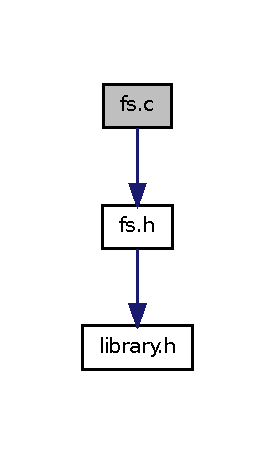
\includegraphics[width=132pt]{fs_8c__incl}
\end{center}
\end{figure}
\subsection*{Functions}
\begin{DoxyCompactItemize}
\item 
\hyperlink{library_8h_ad7ecf93b77285d9bf039d27fa3f1a588}{u32int} \hyperlink{fs_8c_ab3d2c74eb086c4bebacb846a191821da}{read\_\-fs} (\hyperlink{structnode}{fs\_\-node} $\ast$\hyperlink{structnode}{node}, \hyperlink{library_8h_ad7ecf93b77285d9bf039d27fa3f1a588}{u32int} offset, \hyperlink{library_8h_ad7ecf93b77285d9bf039d27fa3f1a588}{u32int} \hyperlink{multiboot_8h_a8c5ccb4d457cb24df33a7c9facfa2650}{size}, \hyperlink{library_8h_a1026e682ffdadc1701c42cd44ce9efcf}{u8int} $\ast$buffer)
\item 
\hyperlink{library_8h_ad7ecf93b77285d9bf039d27fa3f1a588}{u32int} \hyperlink{fs_8c_a85297dd9ef416c6be74dafb32a18661c}{write\_\-fs} (\hyperlink{structnode}{fs\_\-node} $\ast$\hyperlink{structnode}{node}, \hyperlink{library_8h_ad7ecf93b77285d9bf039d27fa3f1a588}{u32int} offset, \hyperlink{library_8h_ad7ecf93b77285d9bf039d27fa3f1a588}{u32int} \hyperlink{multiboot_8h_a8c5ccb4d457cb24df33a7c9facfa2650}{size}, \hyperlink{library_8h_a1026e682ffdadc1701c42cd44ce9efcf}{u8int} $\ast$buffer)
\item 
void \hyperlink{fs_8c_a0d30b35364e5c886a177bca4e8a04da4}{open\_\-fs} (\hyperlink{structnode}{fs\_\-node} $\ast$\hyperlink{structnode}{node}, \hyperlink{library_8h_a1026e682ffdadc1701c42cd44ce9efcf}{u8int} read, \hyperlink{library_8h_a1026e682ffdadc1701c42cd44ce9efcf}{u8int} write)
\item 
void \hyperlink{fs_8c_a688f92b44d9e3ec4c18cae7c3983ec1e}{close\_\-fs} (\hyperlink{structnode}{fs\_\-node} $\ast$\hyperlink{structnode}{node})
\item 
struct \hyperlink{structdirent}{dirent} $\ast$ \hyperlink{fs_8c_ac6b382e12dc9d7aa837ede369fb41e8e}{readdir\_\-fs} (\hyperlink{structnode}{fs\_\-node} $\ast$\hyperlink{structnode}{node}, \hyperlink{library_8h_ad7ecf93b77285d9bf039d27fa3f1a588}{u32int} i)
\item 
\hyperlink{structnode}{fs\_\-node} $\ast$ \hyperlink{fs_8c_a9eb6f75aeaa6c2101297626899532ab7}{finddir\_\-fs} (\hyperlink{structnode}{fs\_\-node} $\ast$\hyperlink{structnode}{node}, char $\ast$name)
\end{DoxyCompactItemize}
\subsection*{Variables}
\begin{DoxyCompactItemize}
\item 
\hyperlink{structnode}{fs\_\-node} $\ast$ \hyperlink{fs_8c_a7e111d5b30877270594a4880df252cff}{root} = 0
\end{DoxyCompactItemize}


\subsection{Function Documentation}
\hypertarget{fs_8c_a688f92b44d9e3ec4c18cae7c3983ec1e}{
\index{fs.c@{fs.c}!close\_\-fs@{close\_\-fs}}
\index{close\_\-fs@{close\_\-fs}!fs.c@{fs.c}}
\subsubsection[{close\_\-fs}]{\setlength{\rightskip}{0pt plus 5cm}void close\_\-fs (
\begin{DoxyParamCaption}
\item[{{\bf fs\_\-node} $\ast$}]{ node}
\end{DoxyParamCaption}
)}}
\label{fs_8c_a688f92b44d9e3ec4c18cae7c3983ec1e}
\hypertarget{fs_8c_a9eb6f75aeaa6c2101297626899532ab7}{
\index{fs.c@{fs.c}!finddir\_\-fs@{finddir\_\-fs}}
\index{finddir\_\-fs@{finddir\_\-fs}!fs.c@{fs.c}}
\subsubsection[{finddir\_\-fs}]{\setlength{\rightskip}{0pt plus 5cm}{\bf fs\_\-node}$\ast$ finddir\_\-fs (
\begin{DoxyParamCaption}
\item[{{\bf fs\_\-node} $\ast$}]{ node, }
\item[{char $\ast$}]{ name}
\end{DoxyParamCaption}
)}}
\label{fs_8c_a9eb6f75aeaa6c2101297626899532ab7}


Here is the caller graph for this function:
\nopagebreak
\begin{figure}[H]
\begin{center}
\leavevmode
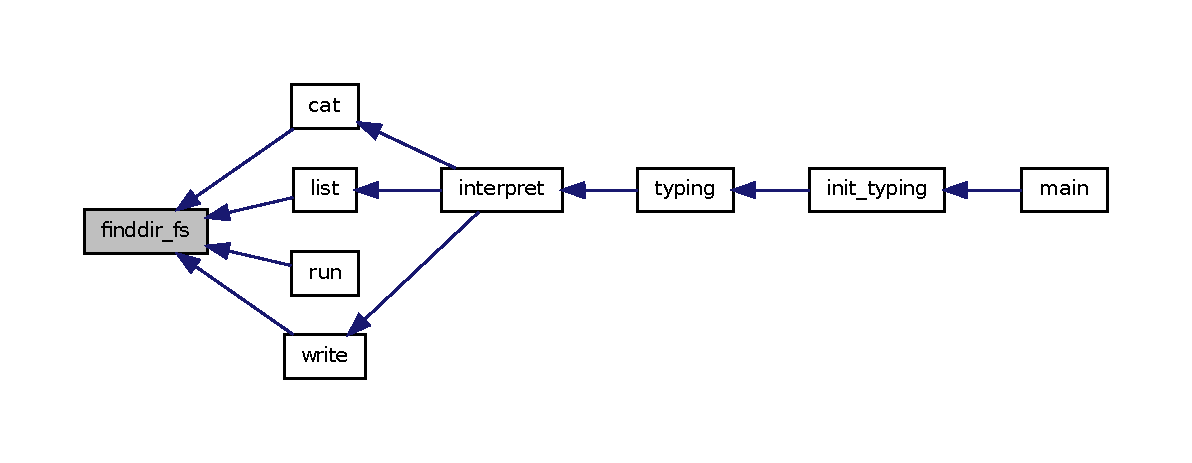
\includegraphics[width=400pt]{fs_8c_a9eb6f75aeaa6c2101297626899532ab7_icgraph}
\end{center}
\end{figure}


\hypertarget{fs_8c_a0d30b35364e5c886a177bca4e8a04da4}{
\index{fs.c@{fs.c}!open\_\-fs@{open\_\-fs}}
\index{open\_\-fs@{open\_\-fs}!fs.c@{fs.c}}
\subsubsection[{open\_\-fs}]{\setlength{\rightskip}{0pt plus 5cm}void open\_\-fs (
\begin{DoxyParamCaption}
\item[{{\bf fs\_\-node} $\ast$}]{ node, }
\item[{{\bf u8int}}]{ read, }
\item[{{\bf u8int}}]{ write}
\end{DoxyParamCaption}
)}}
\label{fs_8c_a0d30b35364e5c886a177bca4e8a04da4}
\hypertarget{fs_8c_ab3d2c74eb086c4bebacb846a191821da}{
\index{fs.c@{fs.c}!read\_\-fs@{read\_\-fs}}
\index{read\_\-fs@{read\_\-fs}!fs.c@{fs.c}}
\subsubsection[{read\_\-fs}]{\setlength{\rightskip}{0pt plus 5cm}{\bf u32int} read\_\-fs (
\begin{DoxyParamCaption}
\item[{{\bf fs\_\-node} $\ast$}]{ node, }
\item[{{\bf u32int}}]{ offset, }
\item[{{\bf u32int}}]{ size, }
\item[{{\bf u8int} $\ast$}]{ buffer}
\end{DoxyParamCaption}
)}}
\label{fs_8c_ab3d2c74eb086c4bebacb846a191821da}


Here is the caller graph for this function:
\nopagebreak
\begin{figure}[H]
\begin{center}
\leavevmode
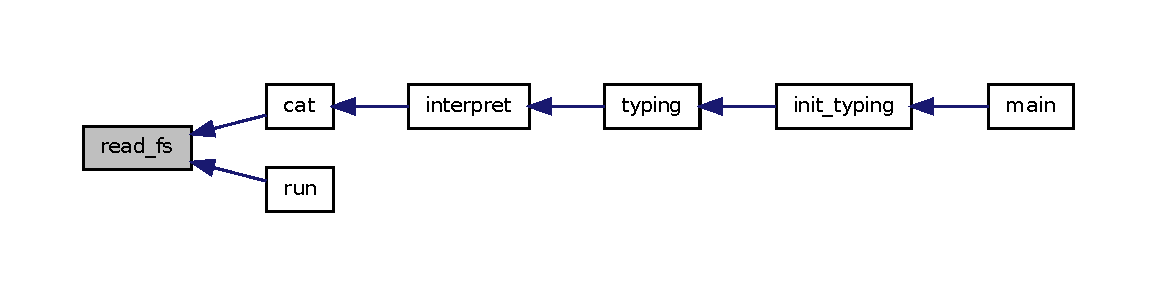
\includegraphics[width=400pt]{fs_8c_ab3d2c74eb086c4bebacb846a191821da_icgraph}
\end{center}
\end{figure}


\hypertarget{fs_8c_ac6b382e12dc9d7aa837ede369fb41e8e}{
\index{fs.c@{fs.c}!readdir\_\-fs@{readdir\_\-fs}}
\index{readdir\_\-fs@{readdir\_\-fs}!fs.c@{fs.c}}
\subsubsection[{readdir\_\-fs}]{\setlength{\rightskip}{0pt plus 5cm}struct {\bf dirent}$\ast$ readdir\_\-fs (
\begin{DoxyParamCaption}
\item[{{\bf fs\_\-node} $\ast$}]{ node, }
\item[{{\bf u32int}}]{ i}
\end{DoxyParamCaption}
)\hspace{0.3cm}{\ttfamily  \mbox{[}read\mbox{]}}}}
\label{fs_8c_ac6b382e12dc9d7aa837ede369fb41e8e}


Here is the caller graph for this function:
\nopagebreak
\begin{figure}[H]
\begin{center}
\leavevmode
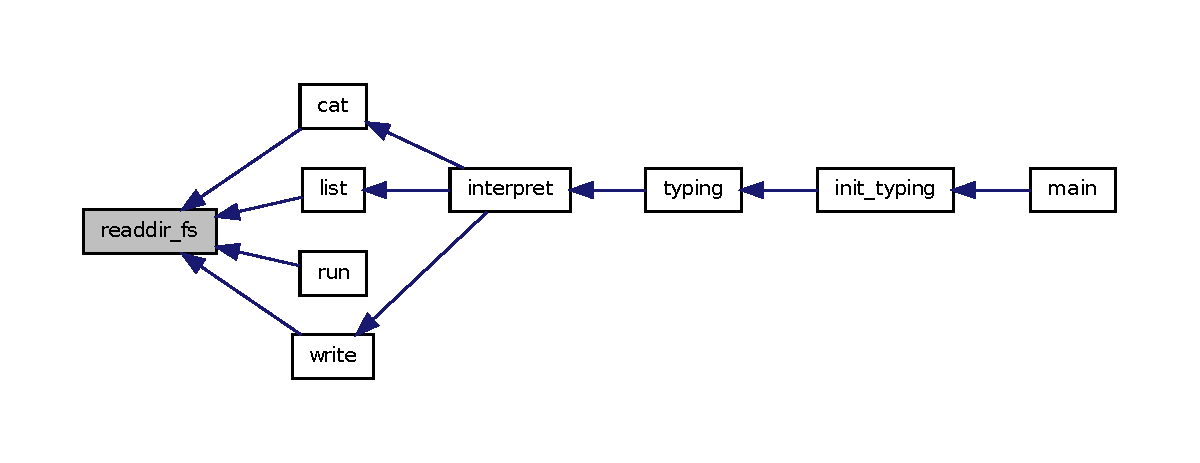
\includegraphics[width=400pt]{fs_8c_ac6b382e12dc9d7aa837ede369fb41e8e_icgraph}
\end{center}
\end{figure}


\hypertarget{fs_8c_a85297dd9ef416c6be74dafb32a18661c}{
\index{fs.c@{fs.c}!write\_\-fs@{write\_\-fs}}
\index{write\_\-fs@{write\_\-fs}!fs.c@{fs.c}}
\subsubsection[{write\_\-fs}]{\setlength{\rightskip}{0pt plus 5cm}{\bf u32int} write\_\-fs (
\begin{DoxyParamCaption}
\item[{{\bf fs\_\-node} $\ast$}]{ node, }
\item[{{\bf u32int}}]{ offset, }
\item[{{\bf u32int}}]{ size, }
\item[{{\bf u8int} $\ast$}]{ buffer}
\end{DoxyParamCaption}
)}}
\label{fs_8c_a85297dd9ef416c6be74dafb32a18661c}


Here is the caller graph for this function:
\nopagebreak
\begin{figure}[H]
\begin{center}
\leavevmode
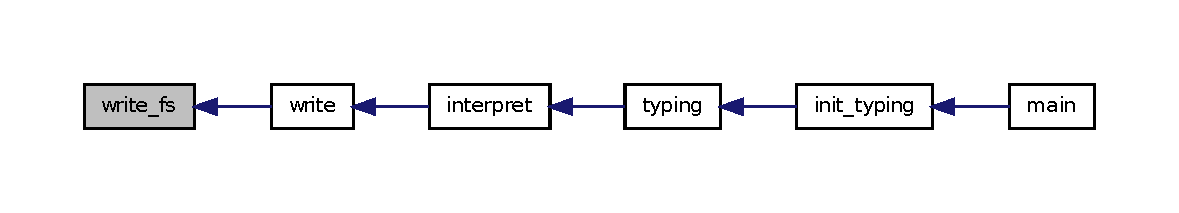
\includegraphics[width=400pt]{fs_8c_a85297dd9ef416c6be74dafb32a18661c_icgraph}
\end{center}
\end{figure}




\subsection{Variable Documentation}
\hypertarget{fs_8c_a7e111d5b30877270594a4880df252cff}{
\index{fs.c@{fs.c}!root@{root}}
\index{root@{root}!fs.c@{fs.c}}
\subsubsection[{root}]{\setlength{\rightskip}{0pt plus 5cm}{\bf fs\_\-node}$\ast$ {\bf root} = 0}}
\label{fs_8c_a7e111d5b30877270594a4880df252cff}

\hypertarget{fs_8h}{
\section{fs.h File Reference}
\label{fs_8h}\index{fs.h@{fs.h}}
}
{\ttfamily \#include \char`\"{}library.h\char`\"{}}\par
Include dependency graph for fs.h:
\nopagebreak
\begin{figure}[H]
\begin{center}
\leavevmode
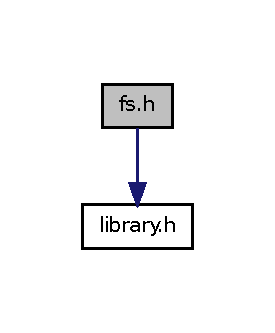
\includegraphics[width=132pt]{fs_8h__incl}
\end{center}
\end{figure}
This graph shows which files directly or indirectly include this file:
\nopagebreak
\begin{figure}[H]
\begin{center}
\leavevmode
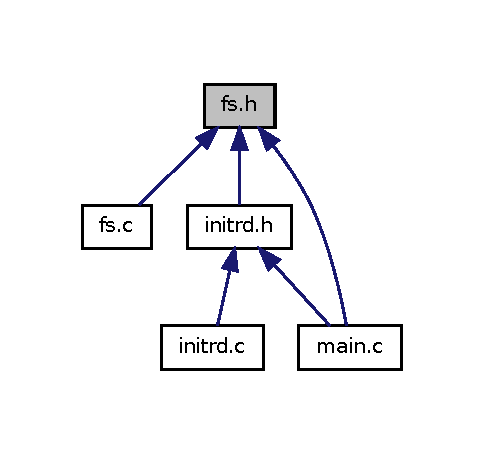
\includegraphics[width=232pt]{fs_8h__dep__incl}
\end{center}
\end{figure}
\subsection*{Data Structures}
\begin{DoxyCompactItemize}
\item 
struct \hyperlink{structnode}{node}
\item 
struct \hyperlink{structdirent}{dirent}
\end{DoxyCompactItemize}
\subsection*{Defines}
\begin{DoxyCompactItemize}
\item 
\#define \hyperlink{fs_8h_a20f0a7ade1270e3923abafeb33864c55}{FS\_\-FILE}~0x01
\item 
\#define \hyperlink{fs_8h_ad7b6b046dfb46cc575f4b9dd418df545}{FS\_\-DIRECTORY}~0x02
\item 
\#define \hyperlink{fs_8h_a5e30957f8b014612f222908bc695ba29}{FS\_\-CHARDEVICE}~0x03
\item 
\#define \hyperlink{fs_8h_aa8e6fa82f33021ca86d48b557a540b7b}{FS\_\-BLOCKDEVICE}~0x04
\item 
\#define \hyperlink{fs_8h_a46ab34c100ed96be6240c4a9af41b517}{FS\_\-PIPE}~0x05
\item 
\#define \hyperlink{fs_8h_acdd896ea040e8df59fc90956cb7813e5}{FS\_\-SYMLINK}~0x06
\item 
\#define \hyperlink{fs_8h_a5bc0261888d6a9d3b88c2d19693627bb}{FS\_\-MOUNTPOINT}~0x08
\end{DoxyCompactItemize}
\subsection*{Typedefs}
\begin{DoxyCompactItemize}
\item 
typedef \hyperlink{library_8h_ad7ecf93b77285d9bf039d27fa3f1a588}{u32int}($\ast$ \hyperlink{fs_8h_ad32b9ac667034d4edf8dc6a9e5306642}{read\_\-type\_\-t} )(struct \hyperlink{structnode}{node} $\ast$, \hyperlink{library_8h_ad7ecf93b77285d9bf039d27fa3f1a588}{u32int}, \hyperlink{library_8h_ad7ecf93b77285d9bf039d27fa3f1a588}{u32int}, \hyperlink{library_8h_a1026e682ffdadc1701c42cd44ce9efcf}{u8int} $\ast$)
\item 
typedef \hyperlink{library_8h_ad7ecf93b77285d9bf039d27fa3f1a588}{u32int}($\ast$ \hyperlink{fs_8h_afbbf89d19d9d2ef84997351f4af5ea2f}{write\_\-type\_\-t} )(struct \hyperlink{structnode}{node} $\ast$, \hyperlink{library_8h_ad7ecf93b77285d9bf039d27fa3f1a588}{u32int}, \hyperlink{library_8h_ad7ecf93b77285d9bf039d27fa3f1a588}{u32int}, \hyperlink{library_8h_a1026e682ffdadc1701c42cd44ce9efcf}{u8int} $\ast$)
\item 
typedef void($\ast$ \hyperlink{fs_8h_a0ef1927acc994d2ab9608eb4eb4308c6}{open\_\-type\_\-t} )(struct \hyperlink{structnode}{node} $\ast$)
\item 
typedef void($\ast$ \hyperlink{fs_8h_aff25a2dc065528aaedb6e2c21cbc7659}{close\_\-type\_\-t} )(struct \hyperlink{structnode}{node} $\ast$)
\item 
typedef struct \hyperlink{structdirent}{dirent} $\ast$($\ast$ \hyperlink{fs_8h_a654cc2a1ada446257b3ef6ac2c1ea7c8}{readdir\_\-type\_\-t} )(struct \hyperlink{structnode}{node} $\ast$, \hyperlink{library_8h_ad7ecf93b77285d9bf039d27fa3f1a588}{u32int})
\item 
typedef struct \hyperlink{structnode}{node} $\ast$($\ast$ \hyperlink{fs_8h_a9961273780df33e576ff4063800f23b4}{finddir\_\-type\_\-t} )(struct \hyperlink{structnode}{node} $\ast$, char $\ast$name)
\item 
typedef struct \hyperlink{structnode}{node} \hyperlink{fs_8h_a837ff8d962b3c1a2d2aa5e0589c47284}{fs\_\-node}
\end{DoxyCompactItemize}
\subsection*{Functions}
\begin{DoxyCompactItemize}
\item 
\hyperlink{library_8h_ad7ecf93b77285d9bf039d27fa3f1a588}{u32int} \hyperlink{fs_8h_ab3d2c74eb086c4bebacb846a191821da}{read\_\-fs} (\hyperlink{structnode}{fs\_\-node} $\ast$\hyperlink{structnode}{node}, \hyperlink{library_8h_ad7ecf93b77285d9bf039d27fa3f1a588}{u32int} offset, \hyperlink{library_8h_ad7ecf93b77285d9bf039d27fa3f1a588}{u32int} \hyperlink{multiboot_8h_a8c5ccb4d457cb24df33a7c9facfa2650}{size}, \hyperlink{library_8h_a1026e682ffdadc1701c42cd44ce9efcf}{u8int} $\ast$buffer)
\item 
\hyperlink{library_8h_ad7ecf93b77285d9bf039d27fa3f1a588}{u32int} \hyperlink{fs_8h_a85297dd9ef416c6be74dafb32a18661c}{write\_\-fs} (\hyperlink{structnode}{fs\_\-node} $\ast$\hyperlink{structnode}{node}, \hyperlink{library_8h_ad7ecf93b77285d9bf039d27fa3f1a588}{u32int} offset, \hyperlink{library_8h_ad7ecf93b77285d9bf039d27fa3f1a588}{u32int} \hyperlink{multiboot_8h_a8c5ccb4d457cb24df33a7c9facfa2650}{size}, \hyperlink{library_8h_a1026e682ffdadc1701c42cd44ce9efcf}{u8int} $\ast$buffer)
\item 
void \hyperlink{fs_8h_a0d30b35364e5c886a177bca4e8a04da4}{open\_\-fs} (\hyperlink{structnode}{fs\_\-node} $\ast$\hyperlink{structnode}{node}, \hyperlink{library_8h_a1026e682ffdadc1701c42cd44ce9efcf}{u8int} read, \hyperlink{library_8h_a1026e682ffdadc1701c42cd44ce9efcf}{u8int} write)
\item 
void \hyperlink{fs_8h_a688f92b44d9e3ec4c18cae7c3983ec1e}{close\_\-fs} (\hyperlink{structnode}{fs\_\-node} $\ast$\hyperlink{structnode}{node})
\item 
struct \hyperlink{structdirent}{dirent} $\ast$ \hyperlink{fs_8h_a4f8680b247e06c3acce3a14f5b6c2ad3}{readdir\_\-fs} (\hyperlink{structnode}{fs\_\-node} $\ast$\hyperlink{structnode}{node}, \hyperlink{library_8h_ad7ecf93b77285d9bf039d27fa3f1a588}{u32int} index)
\item 
\hyperlink{structnode}{fs\_\-node} $\ast$ \hyperlink{fs_8h_a9eb6f75aeaa6c2101297626899532ab7}{finddir\_\-fs} (\hyperlink{structnode}{fs\_\-node} $\ast$\hyperlink{structnode}{node}, char $\ast$name)
\end{DoxyCompactItemize}
\subsection*{Variables}
\begin{DoxyCompactItemize}
\item 
\hyperlink{structnode}{fs\_\-node} $\ast$ \hyperlink{fs_8h_a7e111d5b30877270594a4880df252cff}{root}
\end{DoxyCompactItemize}


\subsection{Define Documentation}
\hypertarget{fs_8h_aa8e6fa82f33021ca86d48b557a540b7b}{
\index{fs.h@{fs.h}!FS\_\-BLOCKDEVICE@{FS\_\-BLOCKDEVICE}}
\index{FS\_\-BLOCKDEVICE@{FS\_\-BLOCKDEVICE}!fs.h@{fs.h}}
\subsubsection[{FS\_\-BLOCKDEVICE}]{\setlength{\rightskip}{0pt plus 5cm}\#define FS\_\-BLOCKDEVICE~0x04}}
\label{fs_8h_aa8e6fa82f33021ca86d48b557a540b7b}
\hypertarget{fs_8h_a5e30957f8b014612f222908bc695ba29}{
\index{fs.h@{fs.h}!FS\_\-CHARDEVICE@{FS\_\-CHARDEVICE}}
\index{FS\_\-CHARDEVICE@{FS\_\-CHARDEVICE}!fs.h@{fs.h}}
\subsubsection[{FS\_\-CHARDEVICE}]{\setlength{\rightskip}{0pt plus 5cm}\#define FS\_\-CHARDEVICE~0x03}}
\label{fs_8h_a5e30957f8b014612f222908bc695ba29}
\hypertarget{fs_8h_ad7b6b046dfb46cc575f4b9dd418df545}{
\index{fs.h@{fs.h}!FS\_\-DIRECTORY@{FS\_\-DIRECTORY}}
\index{FS\_\-DIRECTORY@{FS\_\-DIRECTORY}!fs.h@{fs.h}}
\subsubsection[{FS\_\-DIRECTORY}]{\setlength{\rightskip}{0pt plus 5cm}\#define FS\_\-DIRECTORY~0x02}}
\label{fs_8h_ad7b6b046dfb46cc575f4b9dd418df545}
\hypertarget{fs_8h_a20f0a7ade1270e3923abafeb33864c55}{
\index{fs.h@{fs.h}!FS\_\-FILE@{FS\_\-FILE}}
\index{FS\_\-FILE@{FS\_\-FILE}!fs.h@{fs.h}}
\subsubsection[{FS\_\-FILE}]{\setlength{\rightskip}{0pt plus 5cm}\#define FS\_\-FILE~0x01}}
\label{fs_8h_a20f0a7ade1270e3923abafeb33864c55}
\hypertarget{fs_8h_a5bc0261888d6a9d3b88c2d19693627bb}{
\index{fs.h@{fs.h}!FS\_\-MOUNTPOINT@{FS\_\-MOUNTPOINT}}
\index{FS\_\-MOUNTPOINT@{FS\_\-MOUNTPOINT}!fs.h@{fs.h}}
\subsubsection[{FS\_\-MOUNTPOINT}]{\setlength{\rightskip}{0pt plus 5cm}\#define FS\_\-MOUNTPOINT~0x08}}
\label{fs_8h_a5bc0261888d6a9d3b88c2d19693627bb}
\hypertarget{fs_8h_a46ab34c100ed96be6240c4a9af41b517}{
\index{fs.h@{fs.h}!FS\_\-PIPE@{FS\_\-PIPE}}
\index{FS\_\-PIPE@{FS\_\-PIPE}!fs.h@{fs.h}}
\subsubsection[{FS\_\-PIPE}]{\setlength{\rightskip}{0pt plus 5cm}\#define FS\_\-PIPE~0x05}}
\label{fs_8h_a46ab34c100ed96be6240c4a9af41b517}
\hypertarget{fs_8h_acdd896ea040e8df59fc90956cb7813e5}{
\index{fs.h@{fs.h}!FS\_\-SYMLINK@{FS\_\-SYMLINK}}
\index{FS\_\-SYMLINK@{FS\_\-SYMLINK}!fs.h@{fs.h}}
\subsubsection[{FS\_\-SYMLINK}]{\setlength{\rightskip}{0pt plus 5cm}\#define FS\_\-SYMLINK~0x06}}
\label{fs_8h_acdd896ea040e8df59fc90956cb7813e5}


\subsection{Typedef Documentation}
\hypertarget{fs_8h_aff25a2dc065528aaedb6e2c21cbc7659}{
\index{fs.h@{fs.h}!close\_\-type\_\-t@{close\_\-type\_\-t}}
\index{close\_\-type\_\-t@{close\_\-type\_\-t}!fs.h@{fs.h}}
\subsubsection[{close\_\-type\_\-t}]{\setlength{\rightskip}{0pt plus 5cm}typedef void($\ast$ {\bf close\_\-type\_\-t})(struct {\bf node} $\ast$)}}
\label{fs_8h_aff25a2dc065528aaedb6e2c21cbc7659}
\hypertarget{fs_8h_a9961273780df33e576ff4063800f23b4}{
\index{fs.h@{fs.h}!finddir\_\-type\_\-t@{finddir\_\-type\_\-t}}
\index{finddir\_\-type\_\-t@{finddir\_\-type\_\-t}!fs.h@{fs.h}}
\subsubsection[{finddir\_\-type\_\-t}]{\setlength{\rightskip}{0pt plus 5cm}typedef struct {\bf node}$\ast$($\ast$ {\bf finddir\_\-type\_\-t})(struct {\bf node} $\ast$, char $\ast$name)}}
\label{fs_8h_a9961273780df33e576ff4063800f23b4}
\hypertarget{fs_8h_a837ff8d962b3c1a2d2aa5e0589c47284}{
\index{fs.h@{fs.h}!fs\_\-node@{fs\_\-node}}
\index{fs\_\-node@{fs\_\-node}!fs.h@{fs.h}}
\subsubsection[{fs\_\-node}]{\setlength{\rightskip}{0pt plus 5cm}typedef struct {\bf node}  {\bf fs\_\-node}}}
\label{fs_8h_a837ff8d962b3c1a2d2aa5e0589c47284}
\hypertarget{fs_8h_a0ef1927acc994d2ab9608eb4eb4308c6}{
\index{fs.h@{fs.h}!open\_\-type\_\-t@{open\_\-type\_\-t}}
\index{open\_\-type\_\-t@{open\_\-type\_\-t}!fs.h@{fs.h}}
\subsubsection[{open\_\-type\_\-t}]{\setlength{\rightskip}{0pt plus 5cm}typedef void($\ast$ {\bf open\_\-type\_\-t})(struct {\bf node} $\ast$)}}
\label{fs_8h_a0ef1927acc994d2ab9608eb4eb4308c6}
\hypertarget{fs_8h_ad32b9ac667034d4edf8dc6a9e5306642}{
\index{fs.h@{fs.h}!read\_\-type\_\-t@{read\_\-type\_\-t}}
\index{read\_\-type\_\-t@{read\_\-type\_\-t}!fs.h@{fs.h}}
\subsubsection[{read\_\-type\_\-t}]{\setlength{\rightskip}{0pt plus 5cm}typedef {\bf u32int}($\ast$ {\bf read\_\-type\_\-t})(struct {\bf node} $\ast$, {\bf u32int}, {\bf u32int}, {\bf u8int} $\ast$)}}
\label{fs_8h_ad32b9ac667034d4edf8dc6a9e5306642}
\hypertarget{fs_8h_a654cc2a1ada446257b3ef6ac2c1ea7c8}{
\index{fs.h@{fs.h}!readdir\_\-type\_\-t@{readdir\_\-type\_\-t}}
\index{readdir\_\-type\_\-t@{readdir\_\-type\_\-t}!fs.h@{fs.h}}
\subsubsection[{readdir\_\-type\_\-t}]{\setlength{\rightskip}{0pt plus 5cm}typedef struct {\bf dirent}$\ast$($\ast$ {\bf readdir\_\-type\_\-t})(struct {\bf node} $\ast$, {\bf u32int})}}
\label{fs_8h_a654cc2a1ada446257b3ef6ac2c1ea7c8}
\hypertarget{fs_8h_afbbf89d19d9d2ef84997351f4af5ea2f}{
\index{fs.h@{fs.h}!write\_\-type\_\-t@{write\_\-type\_\-t}}
\index{write\_\-type\_\-t@{write\_\-type\_\-t}!fs.h@{fs.h}}
\subsubsection[{write\_\-type\_\-t}]{\setlength{\rightskip}{0pt plus 5cm}typedef {\bf u32int}($\ast$ {\bf write\_\-type\_\-t})(struct {\bf node} $\ast$, {\bf u32int}, {\bf u32int}, {\bf u8int} $\ast$)}}
\label{fs_8h_afbbf89d19d9d2ef84997351f4af5ea2f}


\subsection{Function Documentation}
\hypertarget{fs_8h_a688f92b44d9e3ec4c18cae7c3983ec1e}{
\index{fs.h@{fs.h}!close\_\-fs@{close\_\-fs}}
\index{close\_\-fs@{close\_\-fs}!fs.h@{fs.h}}
\subsubsection[{close\_\-fs}]{\setlength{\rightskip}{0pt plus 5cm}void close\_\-fs (
\begin{DoxyParamCaption}
\item[{{\bf fs\_\-node} $\ast$}]{ node}
\end{DoxyParamCaption}
)}}
\label{fs_8h_a688f92b44d9e3ec4c18cae7c3983ec1e}
\hypertarget{fs_8h_a9eb6f75aeaa6c2101297626899532ab7}{
\index{fs.h@{fs.h}!finddir\_\-fs@{finddir\_\-fs}}
\index{finddir\_\-fs@{finddir\_\-fs}!fs.h@{fs.h}}
\subsubsection[{finddir\_\-fs}]{\setlength{\rightskip}{0pt plus 5cm}{\bf fs\_\-node}$\ast$ finddir\_\-fs (
\begin{DoxyParamCaption}
\item[{{\bf fs\_\-node} $\ast$}]{ node, }
\item[{char $\ast$}]{ name}
\end{DoxyParamCaption}
)}}
\label{fs_8h_a9eb6f75aeaa6c2101297626899532ab7}


Here is the caller graph for this function:
\nopagebreak
\begin{figure}[H]
\begin{center}
\leavevmode
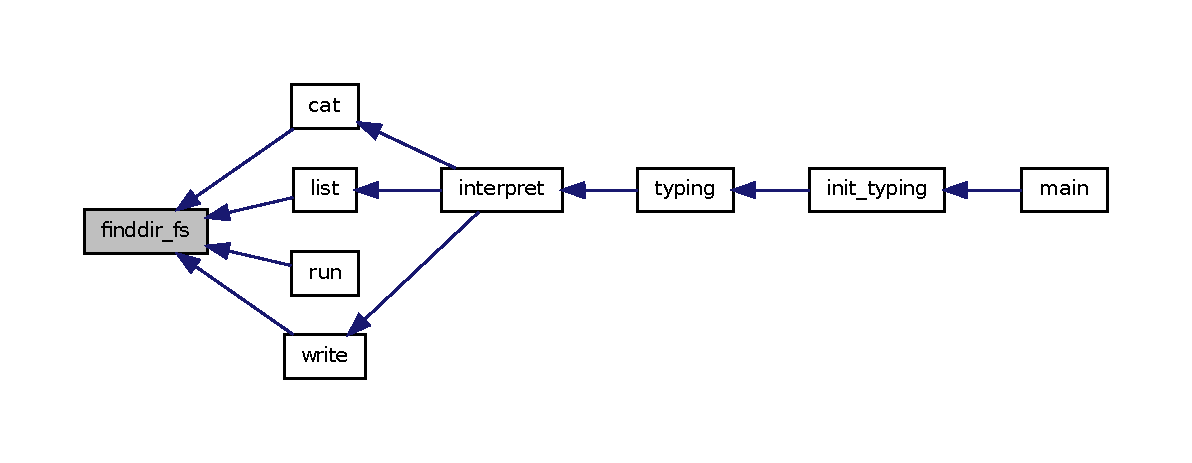
\includegraphics[width=400pt]{fs_8h_a9eb6f75aeaa6c2101297626899532ab7_icgraph}
\end{center}
\end{figure}


\hypertarget{fs_8h_a0d30b35364e5c886a177bca4e8a04da4}{
\index{fs.h@{fs.h}!open\_\-fs@{open\_\-fs}}
\index{open\_\-fs@{open\_\-fs}!fs.h@{fs.h}}
\subsubsection[{open\_\-fs}]{\setlength{\rightskip}{0pt plus 5cm}void open\_\-fs (
\begin{DoxyParamCaption}
\item[{{\bf fs\_\-node} $\ast$}]{ node, }
\item[{{\bf u8int}}]{ read, }
\item[{{\bf u8int}}]{ write}
\end{DoxyParamCaption}
)}}
\label{fs_8h_a0d30b35364e5c886a177bca4e8a04da4}
\hypertarget{fs_8h_ab3d2c74eb086c4bebacb846a191821da}{
\index{fs.h@{fs.h}!read\_\-fs@{read\_\-fs}}
\index{read\_\-fs@{read\_\-fs}!fs.h@{fs.h}}
\subsubsection[{read\_\-fs}]{\setlength{\rightskip}{0pt plus 5cm}{\bf u32int} read\_\-fs (
\begin{DoxyParamCaption}
\item[{{\bf fs\_\-node} $\ast$}]{ node, }
\item[{{\bf u32int}}]{ offset, }
\item[{{\bf u32int}}]{ size, }
\item[{{\bf u8int} $\ast$}]{ buffer}
\end{DoxyParamCaption}
)}}
\label{fs_8h_ab3d2c74eb086c4bebacb846a191821da}


Here is the caller graph for this function:
\nopagebreak
\begin{figure}[H]
\begin{center}
\leavevmode
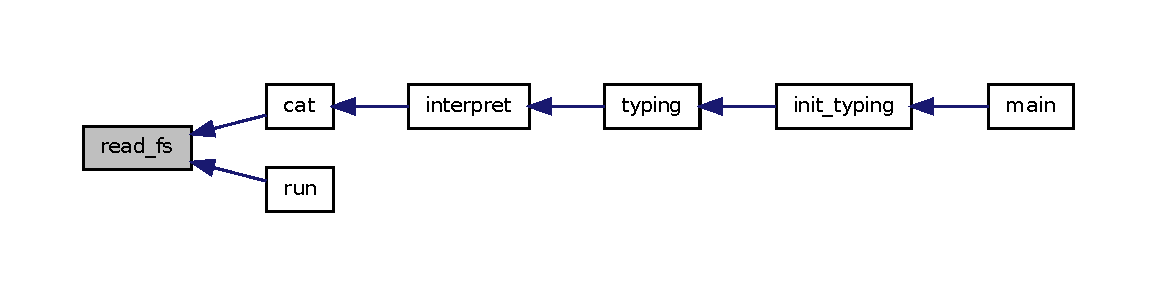
\includegraphics[width=400pt]{fs_8h_ab3d2c74eb086c4bebacb846a191821da_icgraph}
\end{center}
\end{figure}


\hypertarget{fs_8h_a4f8680b247e06c3acce3a14f5b6c2ad3}{
\index{fs.h@{fs.h}!readdir\_\-fs@{readdir\_\-fs}}
\index{readdir\_\-fs@{readdir\_\-fs}!fs.h@{fs.h}}
\subsubsection[{readdir\_\-fs}]{\setlength{\rightskip}{0pt plus 5cm}struct {\bf dirent}$\ast$ readdir\_\-fs (
\begin{DoxyParamCaption}
\item[{{\bf fs\_\-node} $\ast$}]{ node, }
\item[{{\bf u32int}}]{ index}
\end{DoxyParamCaption}
)\hspace{0.3cm}{\ttfamily  \mbox{[}read\mbox{]}}}}
\label{fs_8h_a4f8680b247e06c3acce3a14f5b6c2ad3}


Here is the caller graph for this function:
\nopagebreak
\begin{figure}[H]
\begin{center}
\leavevmode
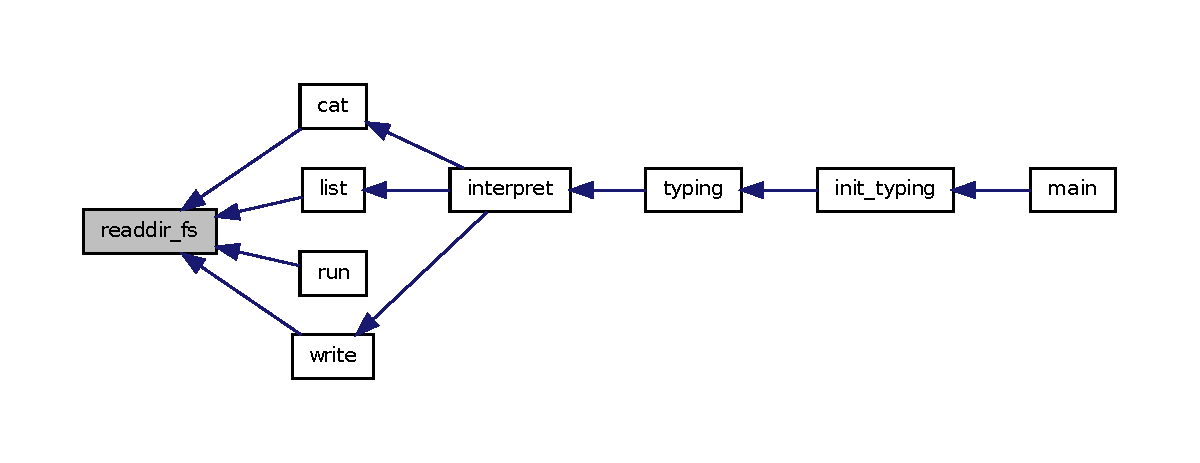
\includegraphics[width=400pt]{fs_8h_a4f8680b247e06c3acce3a14f5b6c2ad3_icgraph}
\end{center}
\end{figure}


\hypertarget{fs_8h_a85297dd9ef416c6be74dafb32a18661c}{
\index{fs.h@{fs.h}!write\_\-fs@{write\_\-fs}}
\index{write\_\-fs@{write\_\-fs}!fs.h@{fs.h}}
\subsubsection[{write\_\-fs}]{\setlength{\rightskip}{0pt plus 5cm}{\bf u32int} write\_\-fs (
\begin{DoxyParamCaption}
\item[{{\bf fs\_\-node} $\ast$}]{ node, }
\item[{{\bf u32int}}]{ offset, }
\item[{{\bf u32int}}]{ size, }
\item[{{\bf u8int} $\ast$}]{ buffer}
\end{DoxyParamCaption}
)}}
\label{fs_8h_a85297dd9ef416c6be74dafb32a18661c}


Here is the caller graph for this function:
\nopagebreak
\begin{figure}[H]
\begin{center}
\leavevmode
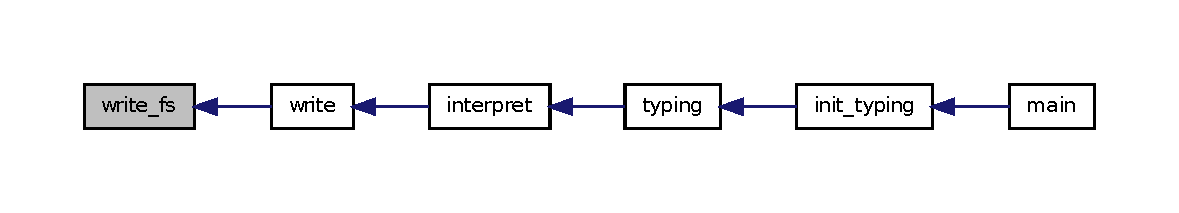
\includegraphics[width=400pt]{fs_8h_a85297dd9ef416c6be74dafb32a18661c_icgraph}
\end{center}
\end{figure}




\subsection{Variable Documentation}
\hypertarget{fs_8h_a7e111d5b30877270594a4880df252cff}{
\index{fs.h@{fs.h}!root@{root}}
\index{root@{root}!fs.h@{fs.h}}
\subsubsection[{root}]{\setlength{\rightskip}{0pt plus 5cm}{\bf fs\_\-node}$\ast$ {\bf root}}}
\label{fs_8h_a7e111d5b30877270594a4880df252cff}

\hypertarget{initrd_8c}{
\section{initrd.c File Reference}
\label{initrd_8c}\index{initrd.c@{initrd.c}}
}
{\ttfamily \#include \char`\"{}initrd.h\char`\"{}}\par
Include dependency graph for initrd.c:
\nopagebreak
\begin{figure}[H]
\begin{center}
\leavevmode
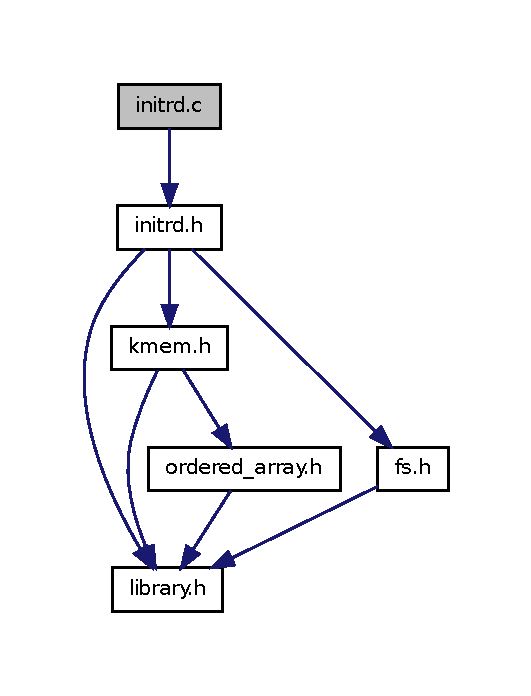
\includegraphics[width=255pt]{initrd_8c__incl}
\end{center}
\end{figure}
\subsection*{Functions}
\begin{DoxyCompactItemize}
\item 
\hyperlink{structnode}{fs\_\-node} $\ast$ \hyperlink{initrd_8c_a9666df78f72f566cb55f7adee3070432}{init\_\-initrd} (\hyperlink{library_8h_ad7ecf93b77285d9bf039d27fa3f1a588}{u32int} location)
\end{DoxyCompactItemize}
\subsection*{Variables}
\begin{DoxyCompactItemize}
\item 
\hyperlink{structinitrd__header}{initrd\_\-header} $\ast$ \hyperlink{initrd_8c_a38331e3c47b8d2fe263d0a26e636e56f}{header}
\item 
\hyperlink{structinitrd__file__header}{initrd\_\-file\_\-header} $\ast$ \hyperlink{initrd_8c_a0dfe59ff327e2e52a8f499cc1c586781}{file\_\-headers}
\item 
\hyperlink{structnode}{fs\_\-node} $\ast$ \hyperlink{initrd_8c_ad7b73422b0131752d98d17fc34bcc850}{initrd\_\-root}
\item 
\hyperlink{structnode}{fs\_\-node} $\ast$ \hyperlink{initrd_8c_a24042e073b5e4fe0c9064c7edd73c768}{initrd\_\-dev}
\item 
\hyperlink{structnode}{fs\_\-node} $\ast$ \hyperlink{initrd_8c_a3a22110da30a9d86a48fc0b2c710b80e}{root\_\-nodes}
\item 
int \hyperlink{initrd_8c_a5802b6d8bba6cc4f156a5cf3426872d6}{nroot\_\-nodes}
\item 
struct \hyperlink{structdirent}{dirent} \hyperlink{initrd_8c_a85a0945a3cb128517bfcd352d3c43c97}{dirent}
\end{DoxyCompactItemize}


\subsection{Function Documentation}
\hypertarget{initrd_8c_a9666df78f72f566cb55f7adee3070432}{
\index{initrd.c@{initrd.c}!init\_\-initrd@{init\_\-initrd}}
\index{init\_\-initrd@{init\_\-initrd}!initrd.c@{initrd.c}}
\subsubsection[{init\_\-initrd}]{\setlength{\rightskip}{0pt plus 5cm}{\bf fs\_\-node}$\ast$ init\_\-initrd (
\begin{DoxyParamCaption}
\item[{{\bf u32int}}]{ location}
\end{DoxyParamCaption}
)}}
\label{initrd_8c_a9666df78f72f566cb55f7adee3070432}


Here is the call graph for this function:
\nopagebreak
\begin{figure}[H]
\begin{center}
\leavevmode
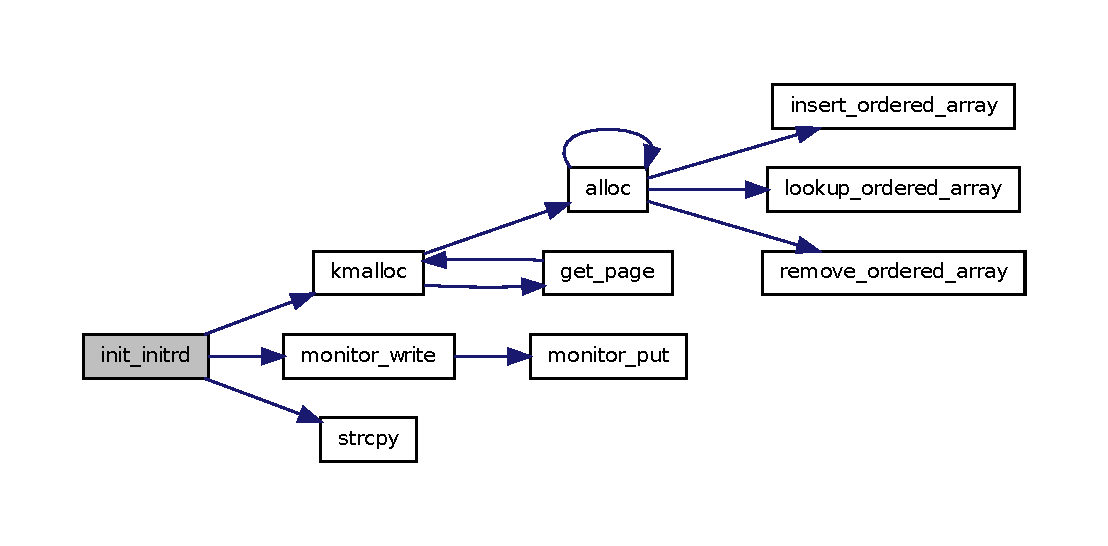
\includegraphics[width=400pt]{initrd_8c_a9666df78f72f566cb55f7adee3070432_cgraph}
\end{center}
\end{figure}




Here is the caller graph for this function:
\nopagebreak
\begin{figure}[H]
\begin{center}
\leavevmode
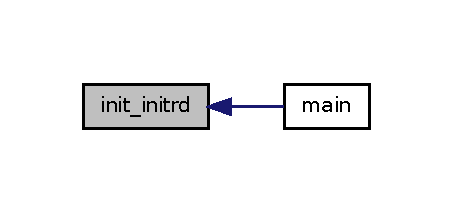
\includegraphics[width=218pt]{initrd_8c_a9666df78f72f566cb55f7adee3070432_icgraph}
\end{center}
\end{figure}




\subsection{Variable Documentation}
\hypertarget{initrd_8c_a85a0945a3cb128517bfcd352d3c43c97}{
\index{initrd.c@{initrd.c}!dirent@{dirent}}
\index{dirent@{dirent}!initrd.c@{initrd.c}}
\subsubsection[{dirent}]{\setlength{\rightskip}{0pt plus 5cm}struct {\bf dirent} {\bf dirent}}}
\label{initrd_8c_a85a0945a3cb128517bfcd352d3c43c97}
\hypertarget{initrd_8c_a0dfe59ff327e2e52a8f499cc1c586781}{
\index{initrd.c@{initrd.c}!file\_\-headers@{file\_\-headers}}
\index{file\_\-headers@{file\_\-headers}!initrd.c@{initrd.c}}
\subsubsection[{file\_\-headers}]{\setlength{\rightskip}{0pt plus 5cm}{\bf initrd\_\-file\_\-header}$\ast$ {\bf file\_\-headers}}}
\label{initrd_8c_a0dfe59ff327e2e52a8f499cc1c586781}
\hypertarget{initrd_8c_a38331e3c47b8d2fe263d0a26e636e56f}{
\index{initrd.c@{initrd.c}!header@{header}}
\index{header@{header}!initrd.c@{initrd.c}}
\subsubsection[{header}]{\setlength{\rightskip}{0pt plus 5cm}{\bf initrd\_\-header}$\ast$ {\bf header}}}
\label{initrd_8c_a38331e3c47b8d2fe263d0a26e636e56f}
\hypertarget{initrd_8c_a24042e073b5e4fe0c9064c7edd73c768}{
\index{initrd.c@{initrd.c}!initrd\_\-dev@{initrd\_\-dev}}
\index{initrd\_\-dev@{initrd\_\-dev}!initrd.c@{initrd.c}}
\subsubsection[{initrd\_\-dev}]{\setlength{\rightskip}{0pt plus 5cm}{\bf fs\_\-node}$\ast$ {\bf initrd\_\-dev}}}
\label{initrd_8c_a24042e073b5e4fe0c9064c7edd73c768}
\hypertarget{initrd_8c_ad7b73422b0131752d98d17fc34bcc850}{
\index{initrd.c@{initrd.c}!initrd\_\-root@{initrd\_\-root}}
\index{initrd\_\-root@{initrd\_\-root}!initrd.c@{initrd.c}}
\subsubsection[{initrd\_\-root}]{\setlength{\rightskip}{0pt plus 5cm}{\bf fs\_\-node}$\ast$ {\bf initrd\_\-root}}}
\label{initrd_8c_ad7b73422b0131752d98d17fc34bcc850}
\hypertarget{initrd_8c_a5802b6d8bba6cc4f156a5cf3426872d6}{
\index{initrd.c@{initrd.c}!nroot\_\-nodes@{nroot\_\-nodes}}
\index{nroot\_\-nodes@{nroot\_\-nodes}!initrd.c@{initrd.c}}
\subsubsection[{nroot\_\-nodes}]{\setlength{\rightskip}{0pt plus 5cm}int {\bf nroot\_\-nodes}}}
\label{initrd_8c_a5802b6d8bba6cc4f156a5cf3426872d6}
\hypertarget{initrd_8c_a3a22110da30a9d86a48fc0b2c710b80e}{
\index{initrd.c@{initrd.c}!root\_\-nodes@{root\_\-nodes}}
\index{root\_\-nodes@{root\_\-nodes}!initrd.c@{initrd.c}}
\subsubsection[{root\_\-nodes}]{\setlength{\rightskip}{0pt plus 5cm}{\bf fs\_\-node}$\ast$ {\bf root\_\-nodes}}}
\label{initrd_8c_a3a22110da30a9d86a48fc0b2c710b80e}

\hypertarget{initrd_8h}{
\section{initrd.h File Reference}
\label{initrd_8h}\index{initrd.h@{initrd.h}}
}
{\ttfamily \#include \char`\"{}library.h\char`\"{}}\par
{\ttfamily \#include \char`\"{}kmem.h\char`\"{}}\par
{\ttfamily \#include \char`\"{}fs.h\char`\"{}}\par
Include dependency graph for initrd.h:
\nopagebreak
\begin{figure}[H]
\begin{center}
\leavevmode
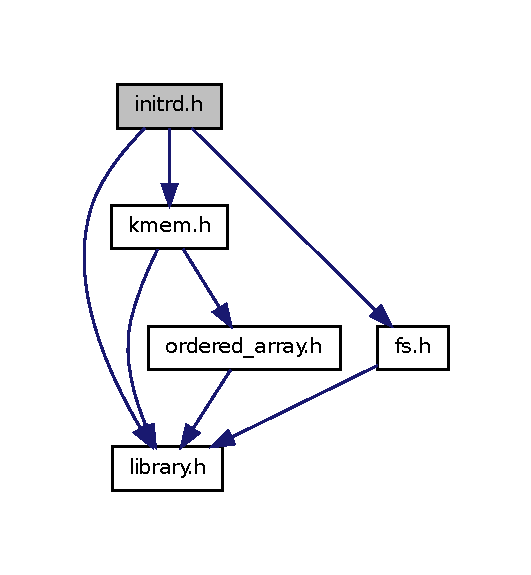
\includegraphics[width=255pt]{initrd_8h__incl}
\end{center}
\end{figure}
This graph shows which files directly or indirectly include this file:
\nopagebreak
\begin{figure}[H]
\begin{center}
\leavevmode
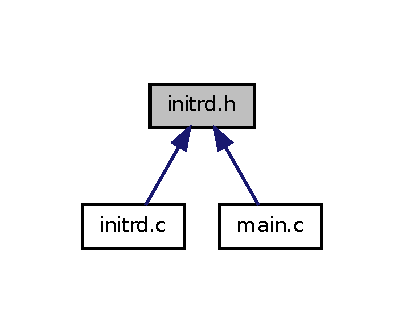
\includegraphics[width=194pt]{initrd_8h__dep__incl}
\end{center}
\end{figure}
\subsection*{Data Structures}
\begin{DoxyCompactItemize}
\item 
struct \hyperlink{structinitrd__header}{initrd\_\-header}
\item 
struct \hyperlink{structinitrd__file__header}{initrd\_\-file\_\-header}
\end{DoxyCompactItemize}
\subsection*{Functions}
\begin{DoxyCompactItemize}
\item 
\hyperlink{structnode}{fs\_\-node} $\ast$ \hyperlink{initrd_8h_a9666df78f72f566cb55f7adee3070432}{init\_\-initrd} (\hyperlink{library_8h_ad7ecf93b77285d9bf039d27fa3f1a588}{u32int} location)
\end{DoxyCompactItemize}


\subsection{Function Documentation}
\hypertarget{initrd_8h_a9666df78f72f566cb55f7adee3070432}{
\index{initrd.h@{initrd.h}!init\_\-initrd@{init\_\-initrd}}
\index{init\_\-initrd@{init\_\-initrd}!initrd.h@{initrd.h}}
\subsubsection[{init\_\-initrd}]{\setlength{\rightskip}{0pt plus 5cm}{\bf fs\_\-node}$\ast$ init\_\-initrd (
\begin{DoxyParamCaption}
\item[{{\bf u32int}}]{ location}
\end{DoxyParamCaption}
)}}
\label{initrd_8h_a9666df78f72f566cb55f7adee3070432}


Here is the call graph for this function:
\nopagebreak
\begin{figure}[H]
\begin{center}
\leavevmode
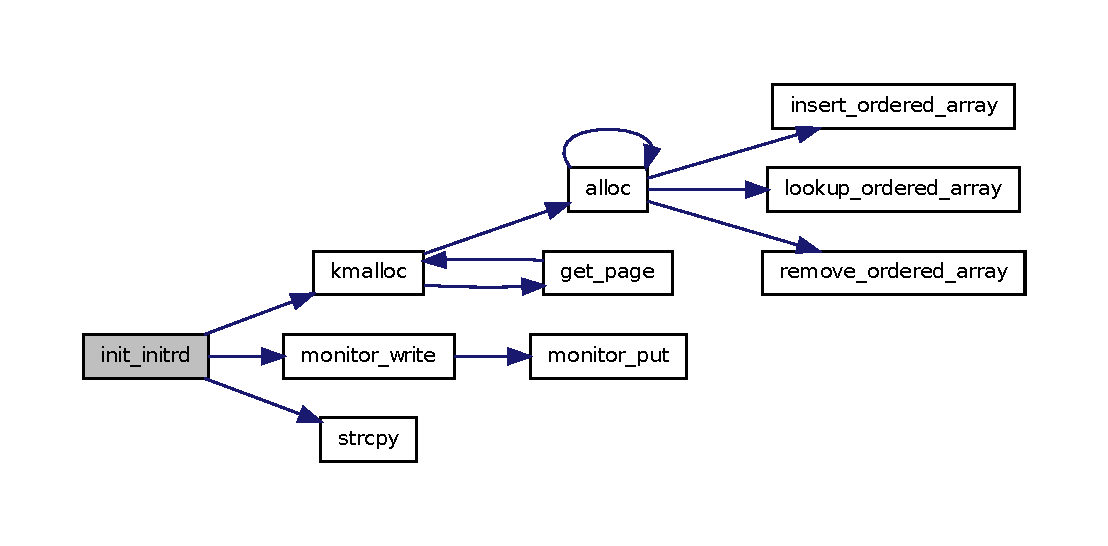
\includegraphics[width=400pt]{initrd_8h_a9666df78f72f566cb55f7adee3070432_cgraph}
\end{center}
\end{figure}




Here is the caller graph for this function:
\nopagebreak
\begin{figure}[H]
\begin{center}
\leavevmode
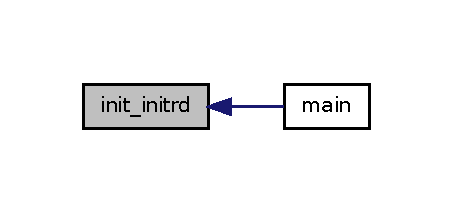
\includegraphics[width=218pt]{initrd_8h_a9666df78f72f566cb55f7adee3070432_icgraph}
\end{center}
\end{figure}



\hypertarget{isr_8c}{
\section{isr.c File Reference}
\label{isr_8c}\index{isr.c@{isr.c}}
}
{\ttfamily \#include \char`\"{}library.h\char`\"{}}\par
{\ttfamily \#include \char`\"{}isr.h\char`\"{}}\par
{\ttfamily \#include \char`\"{}monitor.h\char`\"{}}\par
Include dependency graph for isr.c:
\nopagebreak
\begin{figure}[H]
\begin{center}
\leavevmode
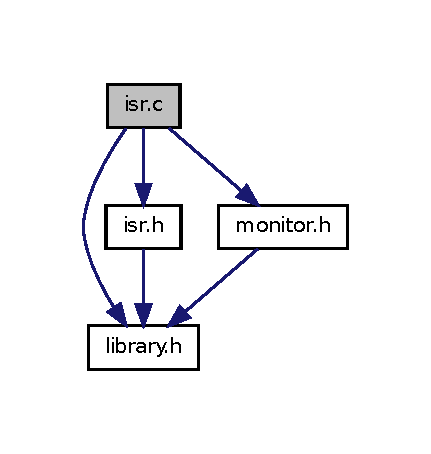
\includegraphics[width=207pt]{isr_8c__incl}
\end{center}
\end{figure}
\subsection*{Functions}
\begin{DoxyCompactItemize}
\item 
void \hyperlink{isr_8c_a700e3ca056bf69296370f504f2cb6cc8}{isr\_\-handler} (\hyperlink{structregisters}{registers\_\-t} regs)
\item 
void \hyperlink{isr_8c_a4f3d6c92004ced19d9683425eafd03d6}{irq\_\-handler} (\hyperlink{structregisters}{registers\_\-t} regs)
\item 
void \hyperlink{isr_8c_ad7ed61410af379195146753d5b45048e}{register\_\-interrupt\_\-handler} (\hyperlink{library_8h_a1026e682ffdadc1701c42cd44ce9efcf}{u8int} n, \hyperlink{isr_8h_acf628c2f58c1c719fd6f9c879ab5ddf4}{isr\_\-t} handler)
\end{DoxyCompactItemize}
\subsection*{Variables}
\begin{DoxyCompactItemize}
\item 
\hyperlink{isr_8h_acf628c2f58c1c719fd6f9c879ab5ddf4}{isr\_\-t} \hyperlink{isr_8c_aa15ebb2df09c4b116f7eba56e527ac8f}{interrupt\_\-handlers} \mbox{[}256\mbox{]}
\end{DoxyCompactItemize}


\subsection{Function Documentation}
\hypertarget{isr_8c_a4f3d6c92004ced19d9683425eafd03d6}{
\index{isr.c@{isr.c}!irq\_\-handler@{irq\_\-handler}}
\index{irq\_\-handler@{irq\_\-handler}!isr.c@{isr.c}}
\subsubsection[{irq\_\-handler}]{\setlength{\rightskip}{0pt plus 5cm}void irq\_\-handler (
\begin{DoxyParamCaption}
\item[{{\bf registers\_\-t}}]{ regs}
\end{DoxyParamCaption}
)}}
\label{isr_8c_a4f3d6c92004ced19d9683425eafd03d6}


Here is the call graph for this function:
\nopagebreak
\begin{figure}[H]
\begin{center}
\leavevmode
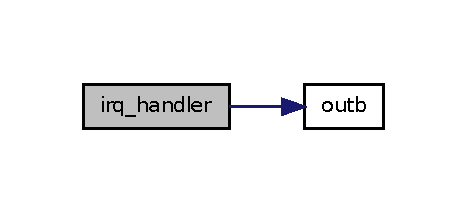
\includegraphics[width=224pt]{isr_8c_a4f3d6c92004ced19d9683425eafd03d6_cgraph}
\end{center}
\end{figure}


\hypertarget{isr_8c_a700e3ca056bf69296370f504f2cb6cc8}{
\index{isr.c@{isr.c}!isr\_\-handler@{isr\_\-handler}}
\index{isr\_\-handler@{isr\_\-handler}!isr.c@{isr.c}}
\subsubsection[{isr\_\-handler}]{\setlength{\rightskip}{0pt plus 5cm}void isr\_\-handler (
\begin{DoxyParamCaption}
\item[{{\bf registers\_\-t}}]{ regs}
\end{DoxyParamCaption}
)}}
\label{isr_8c_a700e3ca056bf69296370f504f2cb6cc8}


Here is the call graph for this function:
\nopagebreak
\begin{figure}[H]
\begin{center}
\leavevmode
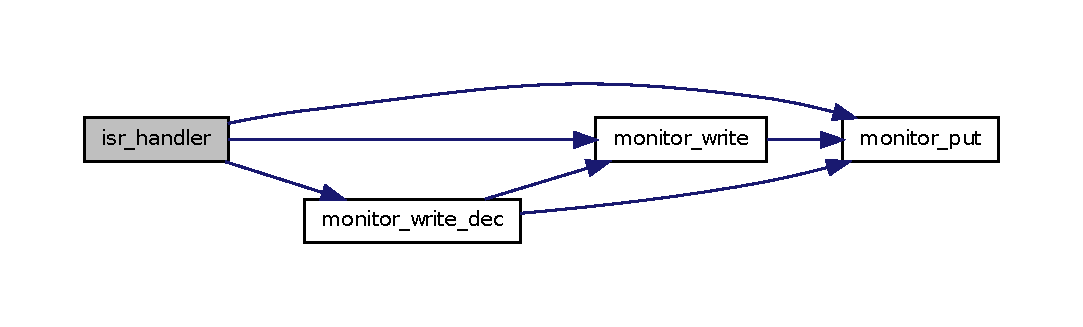
\includegraphics[width=400pt]{isr_8c_a700e3ca056bf69296370f504f2cb6cc8_cgraph}
\end{center}
\end{figure}


\hypertarget{isr_8c_ad7ed61410af379195146753d5b45048e}{
\index{isr.c@{isr.c}!register\_\-interrupt\_\-handler@{register\_\-interrupt\_\-handler}}
\index{register\_\-interrupt\_\-handler@{register\_\-interrupt\_\-handler}!isr.c@{isr.c}}
\subsubsection[{register\_\-interrupt\_\-handler}]{\setlength{\rightskip}{0pt plus 5cm}void register\_\-interrupt\_\-handler (
\begin{DoxyParamCaption}
\item[{{\bf u8int}}]{ n, }
\item[{{\bf isr\_\-t}}]{ handler}
\end{DoxyParamCaption}
)}}
\label{isr_8c_ad7ed61410af379195146753d5b45048e}


Here is the caller graph for this function:
\nopagebreak
\begin{figure}[H]
\begin{center}
\leavevmode
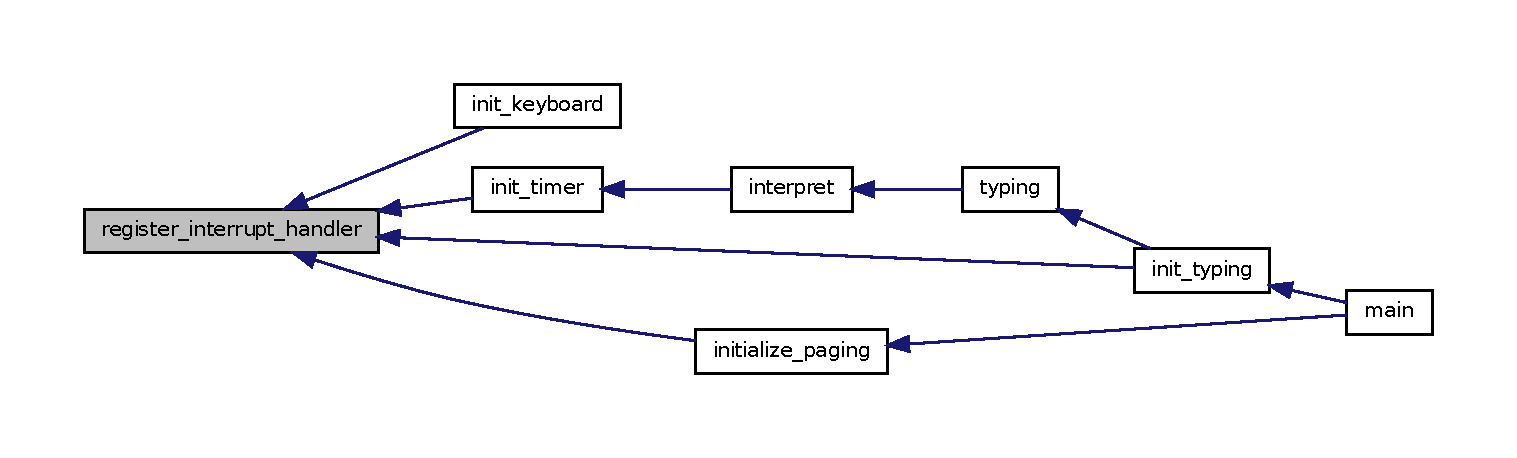
\includegraphics[width=400pt]{isr_8c_ad7ed61410af379195146753d5b45048e_icgraph}
\end{center}
\end{figure}




\subsection{Variable Documentation}
\hypertarget{isr_8c_aa15ebb2df09c4b116f7eba56e527ac8f}{
\index{isr.c@{isr.c}!interrupt\_\-handlers@{interrupt\_\-handlers}}
\index{interrupt\_\-handlers@{interrupt\_\-handlers}!isr.c@{isr.c}}
\subsubsection[{interrupt\_\-handlers}]{\setlength{\rightskip}{0pt plus 5cm}{\bf isr\_\-t} {\bf interrupt\_\-handlers}\mbox{[}256\mbox{]}}}
\label{isr_8c_aa15ebb2df09c4b116f7eba56e527ac8f}

\hypertarget{isr_8h}{
\section{isr.h File Reference}
\label{isr_8h}\index{isr.h@{isr.h}}
}
{\ttfamily \#include \char`\"{}library.h\char`\"{}}\par
Include dependency graph for isr.h:
\nopagebreak
\begin{figure}[H]
\begin{center}
\leavevmode
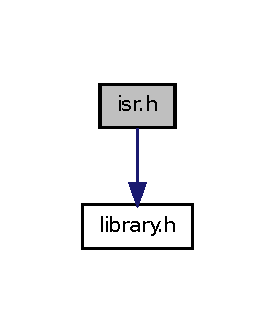
\includegraphics[width=132pt]{isr_8h__incl}
\end{center}
\end{figure}
This graph shows which files directly or indirectly include this file:
\nopagebreak
\begin{figure}[H]
\begin{center}
\leavevmode
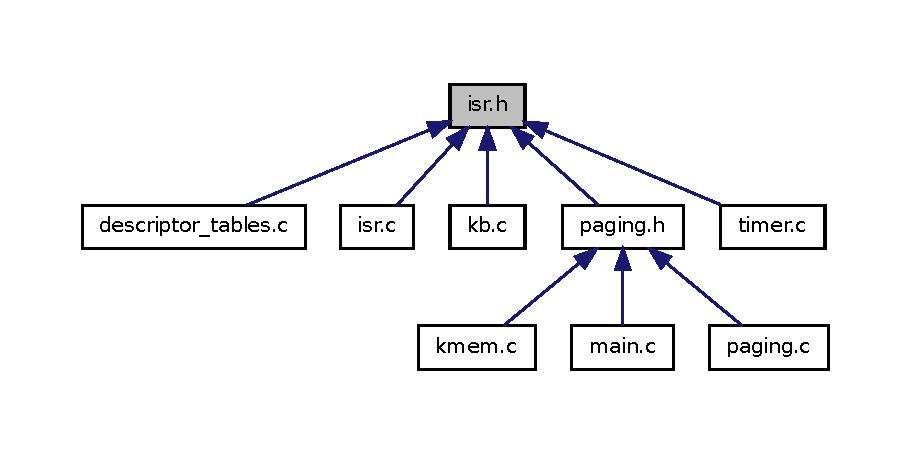
\includegraphics[width=400pt]{isr_8h__dep__incl}
\end{center}
\end{figure}
\subsection*{Data Structures}
\begin{DoxyCompactItemize}
\item 
struct \hyperlink{structregisters}{registers}
\end{DoxyCompactItemize}
\subsection*{Defines}
\begin{DoxyCompactItemize}
\item 
\#define \hyperlink{isr_8h_a8885a13da4dafeb2cb209ce1b7ec3107}{IRQ0}~32
\item 
\#define \hyperlink{isr_8h_a37360776bcc1dd3b5da93b025177551f}{IRQ1}~33
\item 
\#define \hyperlink{isr_8h_a5388784cb69a0b869c4e5f60c839ca24}{IRQ2}~34
\item 
\#define \hyperlink{isr_8h_a81b769ff26428bc3b6f20cb46096f4a2}{IRQ3}~35
\item 
\#define \hyperlink{isr_8h_a3e56e05fa9adf8ddaaf6f44d999017db}{IRQ4}~36
\item 
\#define \hyperlink{isr_8h_af1bd5ba58767b60d0639bd1a096dfdd6}{IRQ5}~37
\item 
\#define \hyperlink{isr_8h_a1282e4c3484ca4c0689e180c5a42a7a9}{IRQ6}~38
\item 
\#define \hyperlink{isr_8h_ac56b9fd6a60941e7594f299521575ca2}{IRQ7}~39
\item 
\#define \hyperlink{isr_8h_ad299f4a78ead6e9f10cfa55376be25ac}{IRQ8}~40
\item 
\#define \hyperlink{isr_8h_af59ffb9e0de6a5a1f9078a110460a2f4}{IRQ9}~41
\item 
\#define \hyperlink{isr_8h_a4937470287000533f2dc2d0c29b88245}{IRQ10}~42
\item 
\#define \hyperlink{isr_8h_afb33d89dcebc322429644b7ce8d3d629}{IRQ11}~43
\item 
\#define \hyperlink{isr_8h_a57276d1481230d81d2bba849f935ce5a}{IRQ12}~44
\item 
\#define \hyperlink{isr_8h_a13f5cba42d2e033d546107a80aa341ea}{IRQ13}~45
\item 
\#define \hyperlink{isr_8h_a9577b9424e1d50ffb437da2a7052f391}{IRQ14}~46
\item 
\#define \hyperlink{isr_8h_a587f058bf281246693f934ab414f7d52}{IRQ15}~47
\end{DoxyCompactItemize}
\subsection*{Typedefs}
\begin{DoxyCompactItemize}
\item 
typedef struct \hyperlink{structregisters}{registers} \hyperlink{isr_8h_adf58dbaf6139b4957c348711f2026957}{registers\_\-t}
\item 
typedef void($\ast$ \hyperlink{isr_8h_acf628c2f58c1c719fd6f9c879ab5ddf4}{isr\_\-t} )(\hyperlink{structregisters}{registers\_\-t})
\end{DoxyCompactItemize}
\subsection*{Functions}
\begin{DoxyCompactItemize}
\item 
void \hyperlink{isr_8h_ad7ed61410af379195146753d5b45048e}{register\_\-interrupt\_\-handler} (\hyperlink{library_8h_a1026e682ffdadc1701c42cd44ce9efcf}{u8int} n, \hyperlink{isr_8h_acf628c2f58c1c719fd6f9c879ab5ddf4}{isr\_\-t} handler)
\end{DoxyCompactItemize}


\subsection{Define Documentation}
\hypertarget{isr_8h_a8885a13da4dafeb2cb209ce1b7ec3107}{
\index{isr.h@{isr.h}!IRQ0@{IRQ0}}
\index{IRQ0@{IRQ0}!isr.h@{isr.h}}
\subsubsection[{IRQ0}]{\setlength{\rightskip}{0pt plus 5cm}\#define IRQ0~32}}
\label{isr_8h_a8885a13da4dafeb2cb209ce1b7ec3107}
\hypertarget{isr_8h_a37360776bcc1dd3b5da93b025177551f}{
\index{isr.h@{isr.h}!IRQ1@{IRQ1}}
\index{IRQ1@{IRQ1}!isr.h@{isr.h}}
\subsubsection[{IRQ1}]{\setlength{\rightskip}{0pt plus 5cm}\#define IRQ1~33}}
\label{isr_8h_a37360776bcc1dd3b5da93b025177551f}
\hypertarget{isr_8h_a4937470287000533f2dc2d0c29b88245}{
\index{isr.h@{isr.h}!IRQ10@{IRQ10}}
\index{IRQ10@{IRQ10}!isr.h@{isr.h}}
\subsubsection[{IRQ10}]{\setlength{\rightskip}{0pt plus 5cm}\#define IRQ10~42}}
\label{isr_8h_a4937470287000533f2dc2d0c29b88245}
\hypertarget{isr_8h_afb33d89dcebc322429644b7ce8d3d629}{
\index{isr.h@{isr.h}!IRQ11@{IRQ11}}
\index{IRQ11@{IRQ11}!isr.h@{isr.h}}
\subsubsection[{IRQ11}]{\setlength{\rightskip}{0pt plus 5cm}\#define IRQ11~43}}
\label{isr_8h_afb33d89dcebc322429644b7ce8d3d629}
\hypertarget{isr_8h_a57276d1481230d81d2bba849f935ce5a}{
\index{isr.h@{isr.h}!IRQ12@{IRQ12}}
\index{IRQ12@{IRQ12}!isr.h@{isr.h}}
\subsubsection[{IRQ12}]{\setlength{\rightskip}{0pt plus 5cm}\#define IRQ12~44}}
\label{isr_8h_a57276d1481230d81d2bba849f935ce5a}
\hypertarget{isr_8h_a13f5cba42d2e033d546107a80aa341ea}{
\index{isr.h@{isr.h}!IRQ13@{IRQ13}}
\index{IRQ13@{IRQ13}!isr.h@{isr.h}}
\subsubsection[{IRQ13}]{\setlength{\rightskip}{0pt plus 5cm}\#define IRQ13~45}}
\label{isr_8h_a13f5cba42d2e033d546107a80aa341ea}
\hypertarget{isr_8h_a9577b9424e1d50ffb437da2a7052f391}{
\index{isr.h@{isr.h}!IRQ14@{IRQ14}}
\index{IRQ14@{IRQ14}!isr.h@{isr.h}}
\subsubsection[{IRQ14}]{\setlength{\rightskip}{0pt plus 5cm}\#define IRQ14~46}}
\label{isr_8h_a9577b9424e1d50ffb437da2a7052f391}
\hypertarget{isr_8h_a587f058bf281246693f934ab414f7d52}{
\index{isr.h@{isr.h}!IRQ15@{IRQ15}}
\index{IRQ15@{IRQ15}!isr.h@{isr.h}}
\subsubsection[{IRQ15}]{\setlength{\rightskip}{0pt plus 5cm}\#define IRQ15~47}}
\label{isr_8h_a587f058bf281246693f934ab414f7d52}
\hypertarget{isr_8h_a5388784cb69a0b869c4e5f60c839ca24}{
\index{isr.h@{isr.h}!IRQ2@{IRQ2}}
\index{IRQ2@{IRQ2}!isr.h@{isr.h}}
\subsubsection[{IRQ2}]{\setlength{\rightskip}{0pt plus 5cm}\#define IRQ2~34}}
\label{isr_8h_a5388784cb69a0b869c4e5f60c839ca24}
\hypertarget{isr_8h_a81b769ff26428bc3b6f20cb46096f4a2}{
\index{isr.h@{isr.h}!IRQ3@{IRQ3}}
\index{IRQ3@{IRQ3}!isr.h@{isr.h}}
\subsubsection[{IRQ3}]{\setlength{\rightskip}{0pt plus 5cm}\#define IRQ3~35}}
\label{isr_8h_a81b769ff26428bc3b6f20cb46096f4a2}
\hypertarget{isr_8h_a3e56e05fa9adf8ddaaf6f44d999017db}{
\index{isr.h@{isr.h}!IRQ4@{IRQ4}}
\index{IRQ4@{IRQ4}!isr.h@{isr.h}}
\subsubsection[{IRQ4}]{\setlength{\rightskip}{0pt plus 5cm}\#define IRQ4~36}}
\label{isr_8h_a3e56e05fa9adf8ddaaf6f44d999017db}
\hypertarget{isr_8h_af1bd5ba58767b60d0639bd1a096dfdd6}{
\index{isr.h@{isr.h}!IRQ5@{IRQ5}}
\index{IRQ5@{IRQ5}!isr.h@{isr.h}}
\subsubsection[{IRQ5}]{\setlength{\rightskip}{0pt plus 5cm}\#define IRQ5~37}}
\label{isr_8h_af1bd5ba58767b60d0639bd1a096dfdd6}
\hypertarget{isr_8h_a1282e4c3484ca4c0689e180c5a42a7a9}{
\index{isr.h@{isr.h}!IRQ6@{IRQ6}}
\index{IRQ6@{IRQ6}!isr.h@{isr.h}}
\subsubsection[{IRQ6}]{\setlength{\rightskip}{0pt plus 5cm}\#define IRQ6~38}}
\label{isr_8h_a1282e4c3484ca4c0689e180c5a42a7a9}
\hypertarget{isr_8h_ac56b9fd6a60941e7594f299521575ca2}{
\index{isr.h@{isr.h}!IRQ7@{IRQ7}}
\index{IRQ7@{IRQ7}!isr.h@{isr.h}}
\subsubsection[{IRQ7}]{\setlength{\rightskip}{0pt plus 5cm}\#define IRQ7~39}}
\label{isr_8h_ac56b9fd6a60941e7594f299521575ca2}
\hypertarget{isr_8h_ad299f4a78ead6e9f10cfa55376be25ac}{
\index{isr.h@{isr.h}!IRQ8@{IRQ8}}
\index{IRQ8@{IRQ8}!isr.h@{isr.h}}
\subsubsection[{IRQ8}]{\setlength{\rightskip}{0pt plus 5cm}\#define IRQ8~40}}
\label{isr_8h_ad299f4a78ead6e9f10cfa55376be25ac}
\hypertarget{isr_8h_af59ffb9e0de6a5a1f9078a110460a2f4}{
\index{isr.h@{isr.h}!IRQ9@{IRQ9}}
\index{IRQ9@{IRQ9}!isr.h@{isr.h}}
\subsubsection[{IRQ9}]{\setlength{\rightskip}{0pt plus 5cm}\#define IRQ9~41}}
\label{isr_8h_af59ffb9e0de6a5a1f9078a110460a2f4}


\subsection{Typedef Documentation}
\hypertarget{isr_8h_acf628c2f58c1c719fd6f9c879ab5ddf4}{
\index{isr.h@{isr.h}!isr\_\-t@{isr\_\-t}}
\index{isr\_\-t@{isr\_\-t}!isr.h@{isr.h}}
\subsubsection[{isr\_\-t}]{\setlength{\rightskip}{0pt plus 5cm}typedef void($\ast$ {\bf isr\_\-t})({\bf registers\_\-t})}}
\label{isr_8h_acf628c2f58c1c719fd6f9c879ab5ddf4}
\hypertarget{isr_8h_adf58dbaf6139b4957c348711f2026957}{
\index{isr.h@{isr.h}!registers\_\-t@{registers\_\-t}}
\index{registers\_\-t@{registers\_\-t}!isr.h@{isr.h}}
\subsubsection[{registers\_\-t}]{\setlength{\rightskip}{0pt plus 5cm}typedef struct {\bf registers}  {\bf registers\_\-t}}}
\label{isr_8h_adf58dbaf6139b4957c348711f2026957}


\subsection{Function Documentation}
\hypertarget{isr_8h_ad7ed61410af379195146753d5b45048e}{
\index{isr.h@{isr.h}!register\_\-interrupt\_\-handler@{register\_\-interrupt\_\-handler}}
\index{register\_\-interrupt\_\-handler@{register\_\-interrupt\_\-handler}!isr.h@{isr.h}}
\subsubsection[{register\_\-interrupt\_\-handler}]{\setlength{\rightskip}{0pt plus 5cm}void register\_\-interrupt\_\-handler (
\begin{DoxyParamCaption}
\item[{{\bf u8int}}]{ n, }
\item[{{\bf isr\_\-t}}]{ handler}
\end{DoxyParamCaption}
)}}
\label{isr_8h_ad7ed61410af379195146753d5b45048e}


Here is the caller graph for this function:
\nopagebreak
\begin{figure}[H]
\begin{center}
\leavevmode
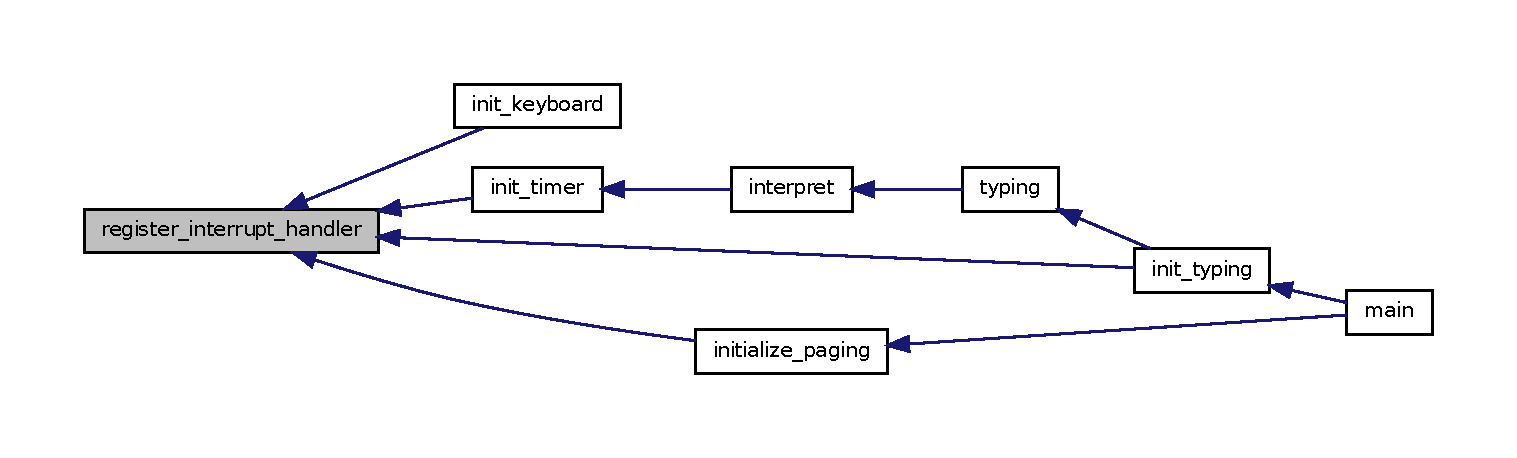
\includegraphics[width=400pt]{isr_8h_ad7ed61410af379195146753d5b45048e_icgraph}
\end{center}
\end{figure}



\hypertarget{kb_8c}{
\section{kb.c File Reference}
\label{kb_8c}\index{kb.c@{kb.c}}
}
{\ttfamily \#include \char`\"{}kb.h\char`\"{}}\par
{\ttfamily \#include \char`\"{}isr.h\char`\"{}}\par
{\ttfamily \#include \char`\"{}timer.h\char`\"{}}\par
{\ttfamily \#include \char`\"{}monitor.h\char`\"{}}\par
Include dependency graph for kb.c:
\nopagebreak
\begin{figure}[H]
\begin{center}
\leavevmode
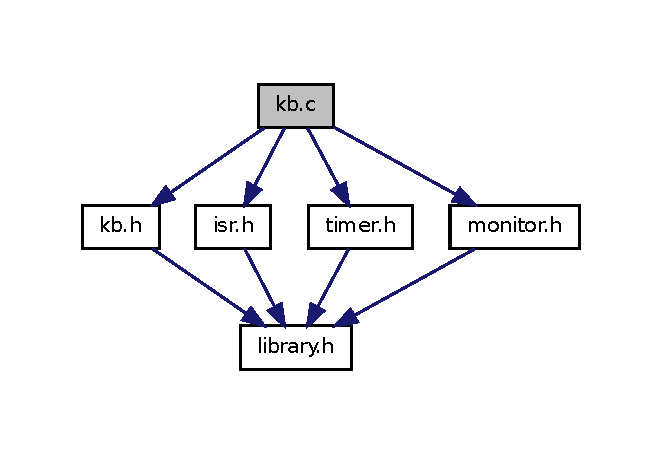
\includegraphics[width=318pt]{kb_8c__incl}
\end{center}
\end{figure}
\subsection*{Functions}
\begin{DoxyCompactItemize}
\item 
unsigned char \hyperlink{kb_8c_a59edcefd8f0e0692f820c30b09a4de71}{key\_\-lookup} (int index)
\item 
void \hyperlink{kb_8c_aed521c3ef126f60e3cd8ba1f90028771}{keyboard\_\-handler} (\hyperlink{structregisters}{registers\_\-t} regs)
\item 
void \hyperlink{kb_8c_ac3a72156d4bbba013e4d62801992794d}{init\_\-keyboard} ()
\end{DoxyCompactItemize}
\subsection*{Variables}
\begin{DoxyCompactItemize}
\item 
unsigned char \hyperlink{kb_8c_aa899d5f48da79692b437a3cf9c475c46}{kbarray} \mbox{[}128\mbox{]}
\end{DoxyCompactItemize}


\subsection{Function Documentation}
\hypertarget{kb_8c_ac3a72156d4bbba013e4d62801992794d}{
\index{kb.c@{kb.c}!init\_\-keyboard@{init\_\-keyboard}}
\index{init\_\-keyboard@{init\_\-keyboard}!kb.c@{kb.c}}
\subsubsection[{init\_\-keyboard}]{\setlength{\rightskip}{0pt plus 5cm}void init\_\-keyboard (
\begin{DoxyParamCaption}
{}
\end{DoxyParamCaption}
)}}
\label{kb_8c_ac3a72156d4bbba013e4d62801992794d}


Here is the call graph for this function:
\nopagebreak
\begin{figure}[H]
\begin{center}
\leavevmode
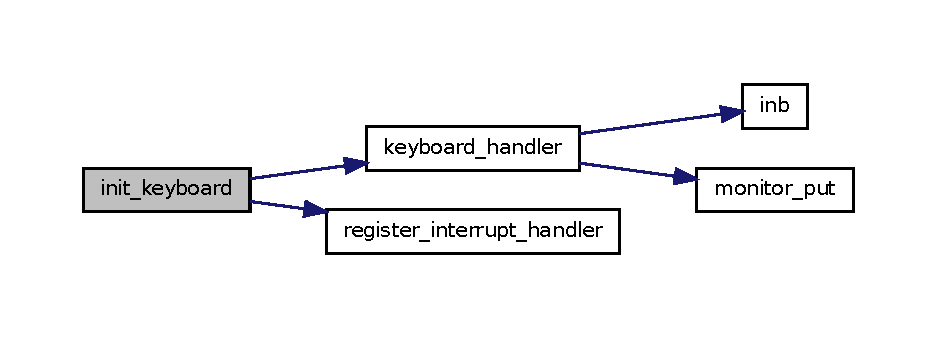
\includegraphics[width=400pt]{kb_8c_ac3a72156d4bbba013e4d62801992794d_cgraph}
\end{center}
\end{figure}


\hypertarget{kb_8c_a59edcefd8f0e0692f820c30b09a4de71}{
\index{kb.c@{kb.c}!key\_\-lookup@{key\_\-lookup}}
\index{key\_\-lookup@{key\_\-lookup}!kb.c@{kb.c}}
\subsubsection[{key\_\-lookup}]{\setlength{\rightskip}{0pt plus 5cm}unsigned char key\_\-lookup (
\begin{DoxyParamCaption}
\item[{int}]{ index}
\end{DoxyParamCaption}
)}}
\label{kb_8c_a59edcefd8f0e0692f820c30b09a4de71}


Here is the caller graph for this function:
\nopagebreak
\begin{figure}[H]
\begin{center}
\leavevmode
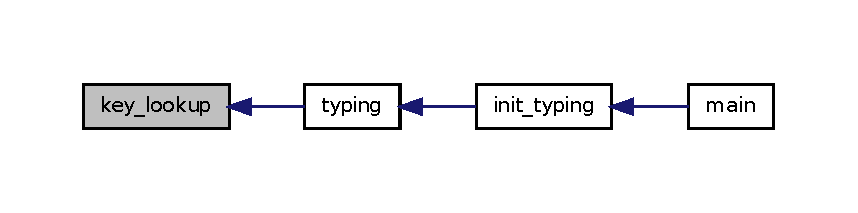
\includegraphics[width=400pt]{kb_8c_a59edcefd8f0e0692f820c30b09a4de71_icgraph}
\end{center}
\end{figure}


\hypertarget{kb_8c_aed521c3ef126f60e3cd8ba1f90028771}{
\index{kb.c@{kb.c}!keyboard\_\-handler@{keyboard\_\-handler}}
\index{keyboard\_\-handler@{keyboard\_\-handler}!kb.c@{kb.c}}
\subsubsection[{keyboard\_\-handler}]{\setlength{\rightskip}{0pt plus 5cm}void keyboard\_\-handler (
\begin{DoxyParamCaption}
\item[{{\bf registers\_\-t}}]{ regs}
\end{DoxyParamCaption}
)}}
\label{kb_8c_aed521c3ef126f60e3cd8ba1f90028771}


Here is the call graph for this function:
\nopagebreak
\begin{figure}[H]
\begin{center}
\leavevmode
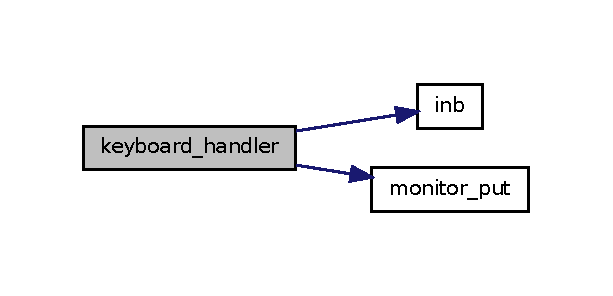
\includegraphics[width=294pt]{kb_8c_aed521c3ef126f60e3cd8ba1f90028771_cgraph}
\end{center}
\end{figure}




Here is the caller graph for this function:
\nopagebreak
\begin{figure}[H]
\begin{center}
\leavevmode
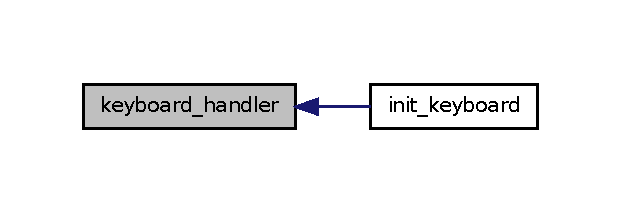
\includegraphics[width=298pt]{kb_8c_aed521c3ef126f60e3cd8ba1f90028771_icgraph}
\end{center}
\end{figure}




\subsection{Variable Documentation}
\hypertarget{kb_8c_aa899d5f48da79692b437a3cf9c475c46}{
\index{kb.c@{kb.c}!kbarray@{kbarray}}
\index{kbarray@{kbarray}!kb.c@{kb.c}}
\subsubsection[{kbarray}]{\setlength{\rightskip}{0pt plus 5cm}unsigned char {\bf kbarray}\mbox{[}128\mbox{]}}}
\label{kb_8c_aa899d5f48da79692b437a3cf9c475c46}

\hypertarget{kb_8h}{
\section{kb.h File Reference}
\label{kb_8h}\index{kb.h@{kb.h}}
}
{\ttfamily \#include \char`\"{}library.h\char`\"{}}\par
Include dependency graph for kb.h:
\nopagebreak
\begin{figure}[H]
\begin{center}
\leavevmode
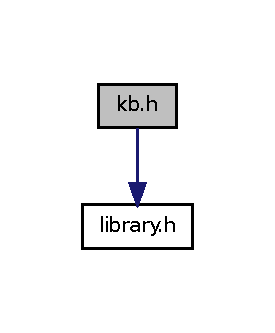
\includegraphics[width=132pt]{kb_8h__incl}
\end{center}
\end{figure}
This graph shows which files directly or indirectly include this file:
\nopagebreak
\begin{figure}[H]
\begin{center}
\leavevmode
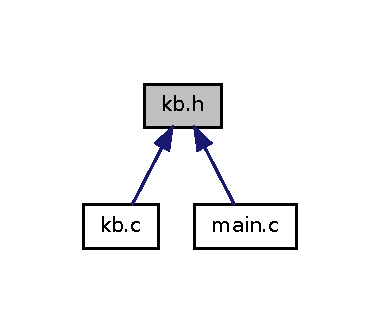
\includegraphics[width=182pt]{kb_8h__dep__incl}
\end{center}
\end{figure}
\subsection*{Functions}
\begin{DoxyCompactItemize}
\item 
unsigned char \hyperlink{kb_8h_a59edcefd8f0e0692f820c30b09a4de71}{key\_\-lookup} (int index)
\item 
void \hyperlink{kb_8h_af112cb1fbdb49ab060a2a4756f15c824}{keyboard\_\-handler} (\hyperlink{structregisters}{registers\_\-t})
\item 
void \hyperlink{kb_8h_abe494366452d929e4478945a46aa70e0}{typing} (\hyperlink{structregisters}{registers\_\-t})
\item 
void \hyperlink{kb_8h_a16c893b53820ad7c0b29142e27b82bd1}{init\_\-typing} ()
\item 
void \hyperlink{kb_8h_ac3a72156d4bbba013e4d62801992794d}{init\_\-keyboard} ()
\end{DoxyCompactItemize}


\subsection{Function Documentation}
\hypertarget{kb_8h_ac3a72156d4bbba013e4d62801992794d}{
\index{kb.h@{kb.h}!init\_\-keyboard@{init\_\-keyboard}}
\index{init\_\-keyboard@{init\_\-keyboard}!kb.h@{kb.h}}
\subsubsection[{init\_\-keyboard}]{\setlength{\rightskip}{0pt plus 5cm}void init\_\-keyboard (
\begin{DoxyParamCaption}
{}
\end{DoxyParamCaption}
)}}
\label{kb_8h_ac3a72156d4bbba013e4d62801992794d}


Here is the call graph for this function:
\nopagebreak
\begin{figure}[H]
\begin{center}
\leavevmode
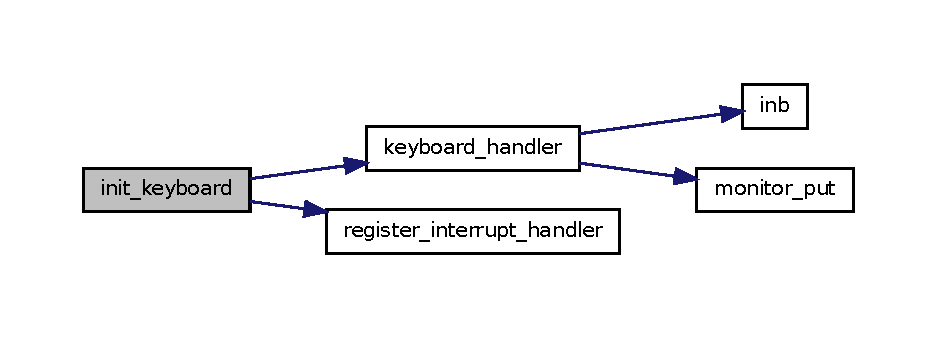
\includegraphics[width=400pt]{kb_8h_ac3a72156d4bbba013e4d62801992794d_cgraph}
\end{center}
\end{figure}


\hypertarget{kb_8h_a16c893b53820ad7c0b29142e27b82bd1}{
\index{kb.h@{kb.h}!init\_\-typing@{init\_\-typing}}
\index{init\_\-typing@{init\_\-typing}!kb.h@{kb.h}}
\subsubsection[{init\_\-typing}]{\setlength{\rightskip}{0pt plus 5cm}void init\_\-typing (
\begin{DoxyParamCaption}
{}
\end{DoxyParamCaption}
)}}
\label{kb_8h_a16c893b53820ad7c0b29142e27b82bd1}


Here is the call graph for this function:
\nopagebreak
\begin{figure}[H]
\begin{center}
\leavevmode
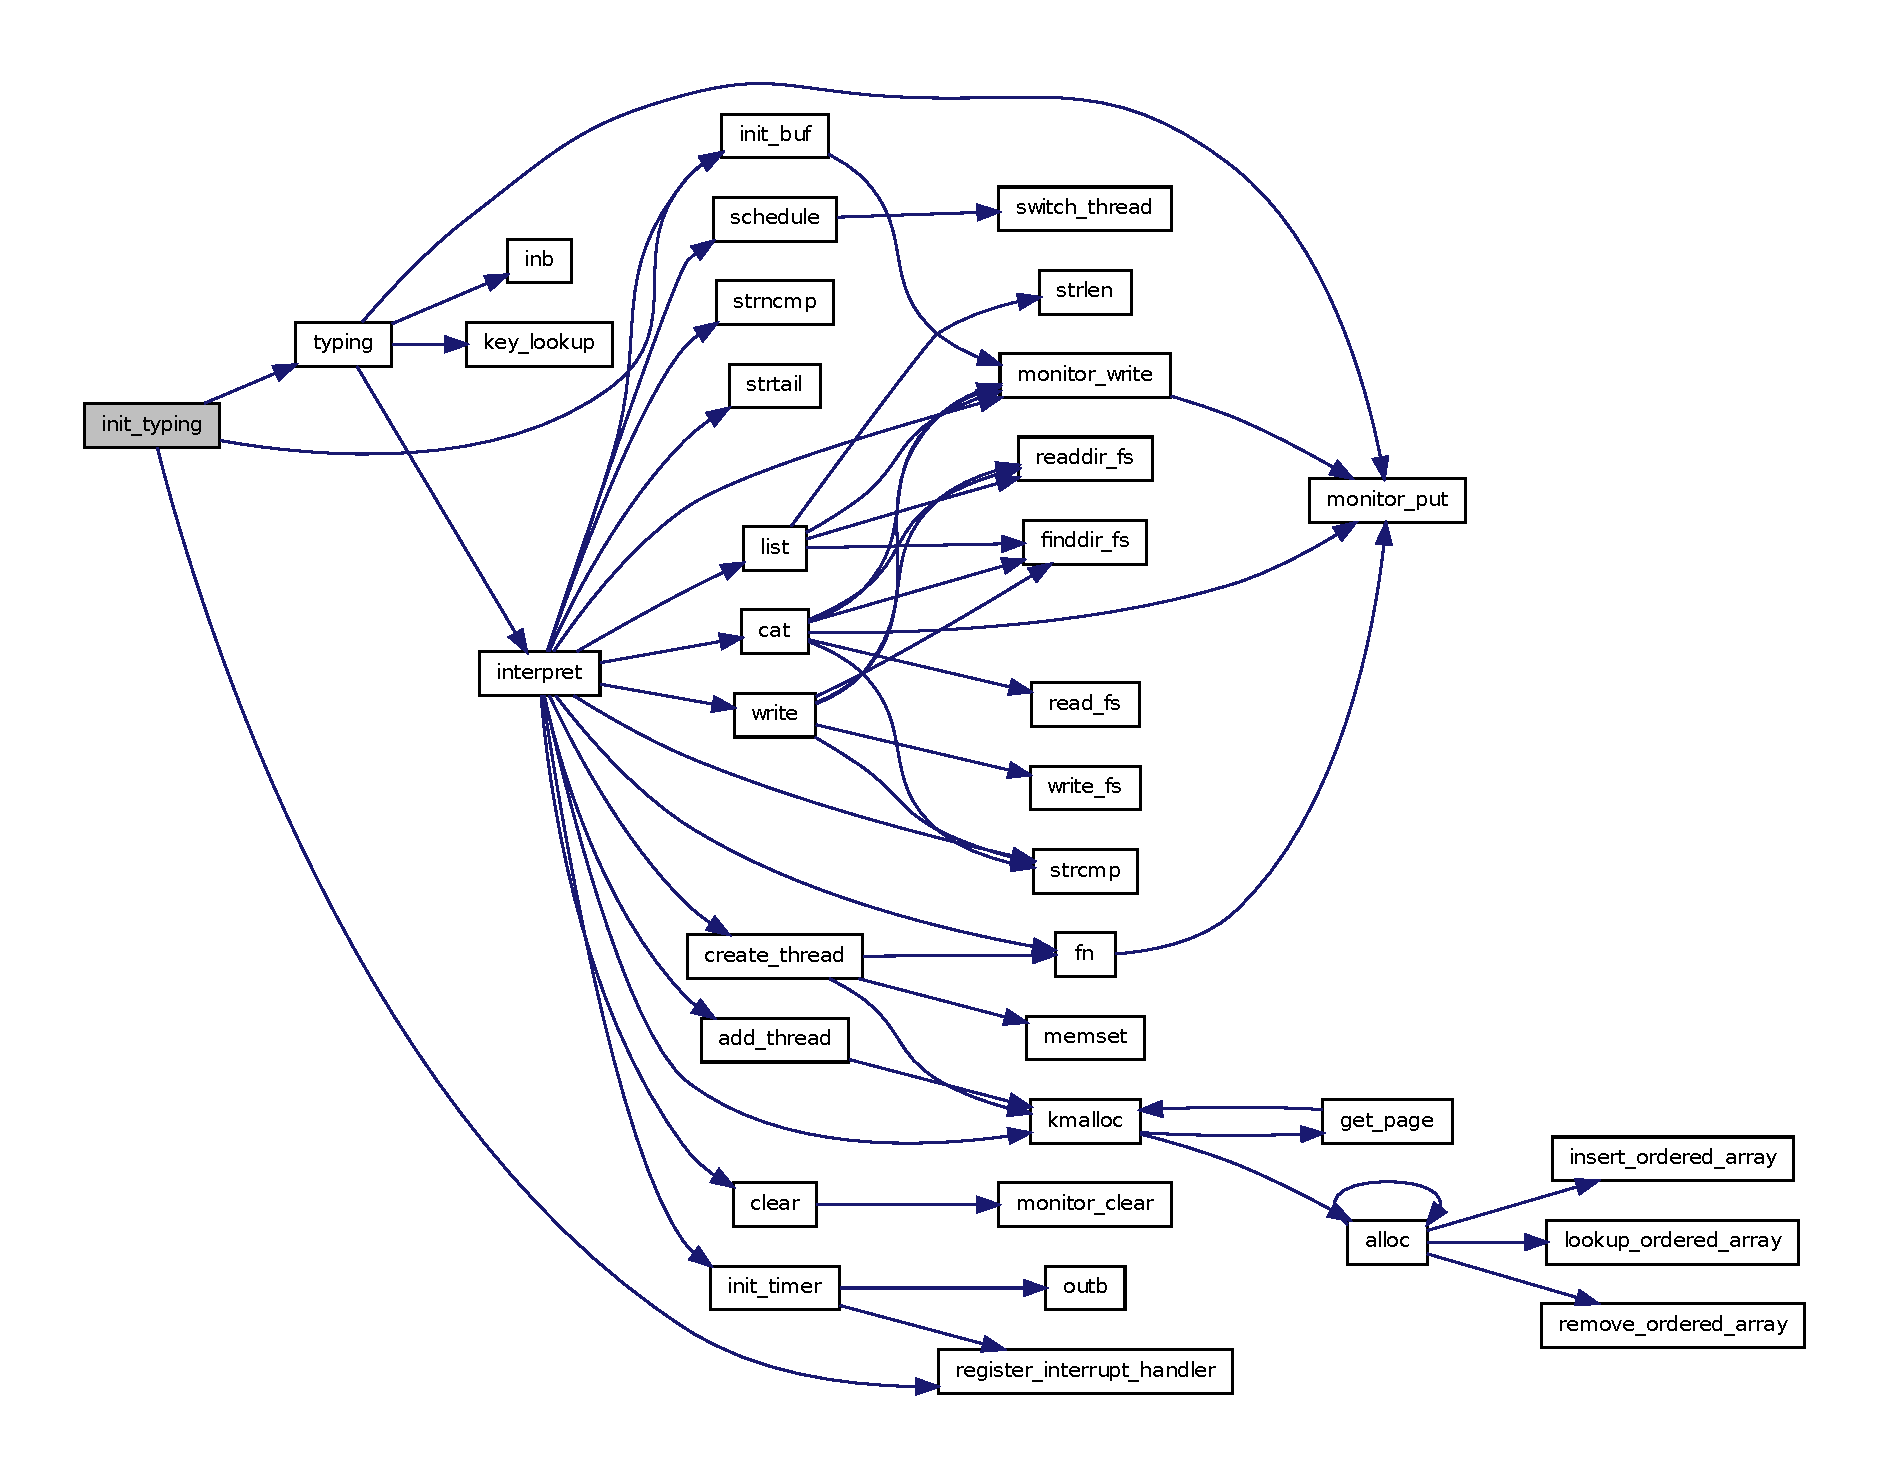
\includegraphics[width=400pt]{kb_8h_a16c893b53820ad7c0b29142e27b82bd1_cgraph}
\end{center}
\end{figure}




Here is the caller graph for this function:
\nopagebreak
\begin{figure}[H]
\begin{center}
\leavevmode
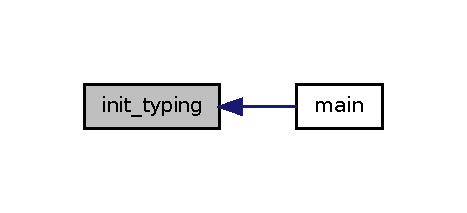
\includegraphics[width=224pt]{kb_8h_a16c893b53820ad7c0b29142e27b82bd1_icgraph}
\end{center}
\end{figure}


\hypertarget{kb_8h_a59edcefd8f0e0692f820c30b09a4de71}{
\index{kb.h@{kb.h}!key\_\-lookup@{key\_\-lookup}}
\index{key\_\-lookup@{key\_\-lookup}!kb.h@{kb.h}}
\subsubsection[{key\_\-lookup}]{\setlength{\rightskip}{0pt plus 5cm}unsigned char key\_\-lookup (
\begin{DoxyParamCaption}
\item[{int}]{ index}
\end{DoxyParamCaption}
)}}
\label{kb_8h_a59edcefd8f0e0692f820c30b09a4de71}


Here is the caller graph for this function:
\nopagebreak
\begin{figure}[H]
\begin{center}
\leavevmode
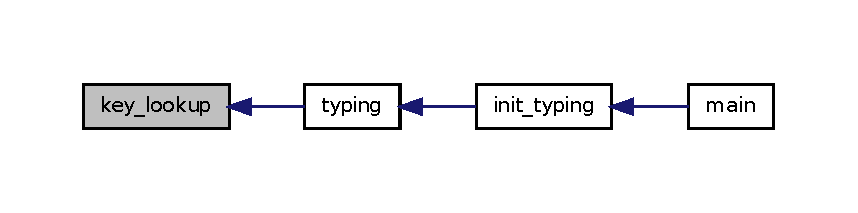
\includegraphics[width=400pt]{kb_8h_a59edcefd8f0e0692f820c30b09a4de71_icgraph}
\end{center}
\end{figure}


\hypertarget{kb_8h_af112cb1fbdb49ab060a2a4756f15c824}{
\index{kb.h@{kb.h}!keyboard\_\-handler@{keyboard\_\-handler}}
\index{keyboard\_\-handler@{keyboard\_\-handler}!kb.h@{kb.h}}
\subsubsection[{keyboard\_\-handler}]{\setlength{\rightskip}{0pt plus 5cm}void keyboard\_\-handler (
\begin{DoxyParamCaption}
\item[{{\bf registers\_\-t}}]{}
\end{DoxyParamCaption}
)}}
\label{kb_8h_af112cb1fbdb49ab060a2a4756f15c824}


Here is the call graph for this function:
\nopagebreak
\begin{figure}[H]
\begin{center}
\leavevmode
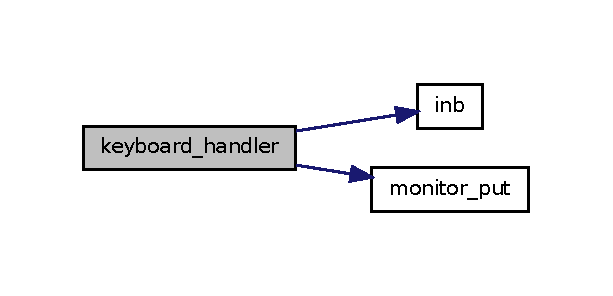
\includegraphics[width=294pt]{kb_8h_af112cb1fbdb49ab060a2a4756f15c824_cgraph}
\end{center}
\end{figure}




Here is the caller graph for this function:
\nopagebreak
\begin{figure}[H]
\begin{center}
\leavevmode
\includegraphics[width=298pt]{kb_8h_af112cb1fbdb49ab060a2a4756f15c824_icgraph}
\end{center}
\end{figure}


\hypertarget{kb_8h_abe494366452d929e4478945a46aa70e0}{
\index{kb.h@{kb.h}!typing@{typing}}
\index{typing@{typing}!kb.h@{kb.h}}
\subsubsection[{typing}]{\setlength{\rightskip}{0pt plus 5cm}void typing (
\begin{DoxyParamCaption}
\item[{{\bf registers\_\-t}}]{}
\end{DoxyParamCaption}
)}}
\label{kb_8h_abe494366452d929e4478945a46aa70e0}


Here is the call graph for this function:
\nopagebreak
\begin{figure}[H]
\begin{center}
\leavevmode
\includegraphics[width=400pt]{kb_8h_abe494366452d929e4478945a46aa70e0_cgraph}
\end{center}
\end{figure}




Here is the caller graph for this function:
\nopagebreak
\begin{figure}[H]
\begin{center}
\leavevmode
\includegraphics[width=306pt]{kb_8h_abe494366452d929e4478945a46aa70e0_icgraph}
\end{center}
\end{figure}



\hypertarget{kmem_8c}{
\section{kmem.c File Reference}
\label{kmem_8c}\index{kmem.c@{kmem.c}}
}
{\ttfamily \#include \char`\"{}kmem.h\char`\"{}}\par
{\ttfamily \#include \char`\"{}paging.h\char`\"{}}\par
Include dependency graph for kmem.c:
\nopagebreak
\begin{figure}[H]
\begin{center}
\leavevmode
\includegraphics[width=277pt]{kmem_8c__incl}
\end{center}
\end{figure}
\subsection*{Functions}
\begin{DoxyCompactItemize}
\item 
\hyperlink{library_8h_ad7ecf93b77285d9bf039d27fa3f1a588}{u32int} \hyperlink{kmem_8c_ae657b8bdbc9148be8fe996a05cc867fc}{kmalloc} (\hyperlink{library_8h_ad7ecf93b77285d9bf039d27fa3f1a588}{u32int} \hyperlink{multiboot_8h_a8c5ccb4d457cb24df33a7c9facfa2650}{size}, int page\_\-align, \hyperlink{library_8h_ad7ecf93b77285d9bf039d27fa3f1a588}{u32int} $\ast$phys)
\item 
void \hyperlink{kmem_8c_af7105034bf054e37218d6ade20db4684}{kfree} (void $\ast$p)
\item 
\hyperlink{structheap__t}{heap\_\-t} $\ast$ \hyperlink{kmem_8c_af2694f380b875f9fc0db5cef82ef6222}{create\_\-heap} (\hyperlink{library_8h_ad7ecf93b77285d9bf039d27fa3f1a588}{u32int} start, \hyperlink{library_8h_ad7ecf93b77285d9bf039d27fa3f1a588}{u32int} end\_\-addr, \hyperlink{library_8h_ad7ecf93b77285d9bf039d27fa3f1a588}{u32int} max, \hyperlink{library_8h_a1026e682ffdadc1701c42cd44ce9efcf}{u8int} supervisor, \hyperlink{library_8h_a1026e682ffdadc1701c42cd44ce9efcf}{u8int} readonly)
\item 
void $\ast$ \hyperlink{kmem_8c_add3c06b419bd2487b79def1ca4784079}{alloc} (\hyperlink{library_8h_ad7ecf93b77285d9bf039d27fa3f1a588}{u32int} \hyperlink{multiboot_8h_a8c5ccb4d457cb24df33a7c9facfa2650}{size}, \hyperlink{library_8h_a1026e682ffdadc1701c42cd44ce9efcf}{u8int} page\_\-align, \hyperlink{structheap__t}{heap\_\-t} $\ast$heap)
\item 
void \hyperlink{kmem_8c_a266d3a15c9fa224ed24a31f38d50a8b8}{free} (void $\ast$p, \hyperlink{structheap__t}{heap\_\-t} $\ast$heap)
\end{DoxyCompactItemize}
\subsection*{Variables}
\begin{DoxyCompactItemize}
\item 
\hyperlink{library_8h_ad7ecf93b77285d9bf039d27fa3f1a588}{u32int} \hyperlink{kmem_8c_a6342e29537636642d9a1477deabf683f}{end}
\item 
\hyperlink{library_8h_ad7ecf93b77285d9bf039d27fa3f1a588}{u32int} \hyperlink{kmem_8c_a1190c85c81abdfbf1fba56ba7d3d78e6}{mem\_\-ptr} = (\hyperlink{library_8h_ad7ecf93b77285d9bf039d27fa3f1a588}{u32int})\&\hyperlink{kmem_8c_a6342e29537636642d9a1477deabf683f}{end}
\item 
\hyperlink{structpage__directory}{page\_\-directory\_\-table} $\ast$ \hyperlink{kmem_8c_a92a6318f506f0e8f68063b71bc445d5f}{kernel\_\-directory}
\item 
\hyperlink{structheap__t}{heap\_\-t} $\ast$ \hyperlink{kmem_8c_a517ce61e492dcf2ae8d2e232a2499a24}{kheap} = 0
\end{DoxyCompactItemize}


\subsection{Function Documentation}
\hypertarget{kmem_8c_add3c06b419bd2487b79def1ca4784079}{
\index{kmem.c@{kmem.c}!alloc@{alloc}}
\index{alloc@{alloc}!kmem.c@{kmem.c}}
\subsubsection[{alloc}]{\setlength{\rightskip}{0pt plus 5cm}void$\ast$ alloc (
\begin{DoxyParamCaption}
\item[{{\bf u32int}}]{ size, }
\item[{{\bf u8int}}]{ page\_\-align, }
\item[{{\bf heap\_\-t} $\ast$}]{ heap}
\end{DoxyParamCaption}
)}}
\label{kmem_8c_add3c06b419bd2487b79def1ca4784079}


Here is the call graph for this function:
\nopagebreak
\begin{figure}[H]
\begin{center}
\leavevmode
\includegraphics[width=283pt]{kmem_8c_add3c06b419bd2487b79def1ca4784079_cgraph}
\end{center}
\end{figure}




Here is the caller graph for this function:
\nopagebreak
\begin{figure}[H]
\begin{center}
\leavevmode
\includegraphics[width=400pt]{kmem_8c_add3c06b419bd2487b79def1ca4784079_icgraph}
\end{center}
\end{figure}


\hypertarget{kmem_8c_af2694f380b875f9fc0db5cef82ef6222}{
\index{kmem.c@{kmem.c}!create\_\-heap@{create\_\-heap}}
\index{create\_\-heap@{create\_\-heap}!kmem.c@{kmem.c}}
\subsubsection[{create\_\-heap}]{\setlength{\rightskip}{0pt plus 5cm}{\bf heap\_\-t}$\ast$ create\_\-heap (
\begin{DoxyParamCaption}
\item[{{\bf u32int}}]{ start, }
\item[{{\bf u32int}}]{ end\_\-addr, }
\item[{{\bf u32int}}]{ max, }
\item[{{\bf u8int}}]{ supervisor, }
\item[{{\bf u8int}}]{ readonly}
\end{DoxyParamCaption}
)}}
\label{kmem_8c_af2694f380b875f9fc0db5cef82ef6222}


Here is the call graph for this function:
\nopagebreak
\begin{figure}[H]
\begin{center}
\leavevmode
\includegraphics[width=400pt]{kmem_8c_af2694f380b875f9fc0db5cef82ef6222_cgraph}
\end{center}
\end{figure}




Here is the caller graph for this function:
\nopagebreak
\begin{figure}[H]
\begin{center}
\leavevmode
\includegraphics[width=364pt]{kmem_8c_af2694f380b875f9fc0db5cef82ef6222_icgraph}
\end{center}
\end{figure}


\hypertarget{kmem_8c_a266d3a15c9fa224ed24a31f38d50a8b8}{
\index{kmem.c@{kmem.c}!free@{free}}
\index{free@{free}!kmem.c@{kmem.c}}
\subsubsection[{free}]{\setlength{\rightskip}{0pt plus 5cm}void free (
\begin{DoxyParamCaption}
\item[{void $\ast$}]{ p, }
\item[{{\bf heap\_\-t} $\ast$}]{ heap}
\end{DoxyParamCaption}
)}}
\label{kmem_8c_a266d3a15c9fa224ed24a31f38d50a8b8}


Here is the call graph for this function:
\nopagebreak
\begin{figure}[H]
\begin{center}
\leavevmode
\includegraphics[width=278pt]{kmem_8c_a266d3a15c9fa224ed24a31f38d50a8b8_cgraph}
\end{center}
\end{figure}




Here is the caller graph for this function:
\nopagebreak
\begin{figure}[H]
\begin{center}
\leavevmode
\includegraphics[width=314pt]{kmem_8c_a266d3a15c9fa224ed24a31f38d50a8b8_icgraph}
\end{center}
\end{figure}


\hypertarget{kmem_8c_af7105034bf054e37218d6ade20db4684}{
\index{kmem.c@{kmem.c}!kfree@{kfree}}
\index{kfree@{kfree}!kmem.c@{kmem.c}}
\subsubsection[{kfree}]{\setlength{\rightskip}{0pt plus 5cm}void kfree (
\begin{DoxyParamCaption}
\item[{void $\ast$}]{ p}
\end{DoxyParamCaption}
)}}
\label{kmem_8c_af7105034bf054e37218d6ade20db4684}


Here is the call graph for this function:
\nopagebreak
\begin{figure}[H]
\begin{center}
\leavevmode
\includegraphics[width=356pt]{kmem_8c_af7105034bf054e37218d6ade20db4684_cgraph}
\end{center}
\end{figure}




Here is the caller graph for this function:
\nopagebreak
\begin{figure}[H]
\begin{center}
\leavevmode
\includegraphics[width=242pt]{kmem_8c_af7105034bf054e37218d6ade20db4684_icgraph}
\end{center}
\end{figure}


\hypertarget{kmem_8c_ae657b8bdbc9148be8fe996a05cc867fc}{
\index{kmem.c@{kmem.c}!kmalloc@{kmalloc}}
\index{kmalloc@{kmalloc}!kmem.c@{kmem.c}}
\subsubsection[{kmalloc}]{\setlength{\rightskip}{0pt plus 5cm}{\bf u32int} kmalloc (
\begin{DoxyParamCaption}
\item[{{\bf u32int}}]{ size, }
\item[{int}]{ page\_\-align, }
\item[{{\bf u32int} $\ast$}]{ phys}
\end{DoxyParamCaption}
)}}
\label{kmem_8c_ae657b8bdbc9148be8fe996a05cc867fc}


Here is the call graph for this function:
\nopagebreak
\begin{figure}[H]
\begin{center}
\leavevmode
\includegraphics[width=394pt]{kmem_8c_ae657b8bdbc9148be8fe996a05cc867fc_cgraph}
\end{center}
\end{figure}




Here is the caller graph for this function:
\nopagebreak
\begin{figure}[H]
\begin{center}
\leavevmode
\includegraphics[width=400pt]{kmem_8c_ae657b8bdbc9148be8fe996a05cc867fc_icgraph}
\end{center}
\end{figure}




\subsection{Variable Documentation}
\hypertarget{kmem_8c_a6342e29537636642d9a1477deabf683f}{
\index{kmem.c@{kmem.c}!end@{end}}
\index{end@{end}!kmem.c@{kmem.c}}
\subsubsection[{end}]{\setlength{\rightskip}{0pt plus 5cm}{\bf u32int} {\bf end}}}
\label{kmem_8c_a6342e29537636642d9a1477deabf683f}
\hypertarget{kmem_8c_a92a6318f506f0e8f68063b71bc445d5f}{
\index{kmem.c@{kmem.c}!kernel\_\-directory@{kernel\_\-directory}}
\index{kernel\_\-directory@{kernel\_\-directory}!kmem.c@{kmem.c}}
\subsubsection[{kernel\_\-directory}]{\setlength{\rightskip}{0pt plus 5cm}{\bf page\_\-directory\_\-table}$\ast$ {\bf kernel\_\-directory}}}
\label{kmem_8c_a92a6318f506f0e8f68063b71bc445d5f}
\hypertarget{kmem_8c_a517ce61e492dcf2ae8d2e232a2499a24}{
\index{kmem.c@{kmem.c}!kheap@{kheap}}
\index{kheap@{kheap}!kmem.c@{kmem.c}}
\subsubsection[{kheap}]{\setlength{\rightskip}{0pt plus 5cm}{\bf heap\_\-t}$\ast$ {\bf kheap} = 0}}
\label{kmem_8c_a517ce61e492dcf2ae8d2e232a2499a24}
\hypertarget{kmem_8c_a1190c85c81abdfbf1fba56ba7d3d78e6}{
\index{kmem.c@{kmem.c}!mem\_\-ptr@{mem\_\-ptr}}
\index{mem\_\-ptr@{mem\_\-ptr}!kmem.c@{kmem.c}}
\subsubsection[{mem\_\-ptr}]{\setlength{\rightskip}{0pt plus 5cm}{\bf u32int} {\bf mem\_\-ptr} = ({\bf u32int})\&{\bf end}}}
\label{kmem_8c_a1190c85c81abdfbf1fba56ba7d3d78e6}

\hypertarget{kmem_8h}{
\section{kmem.h File Reference}
\label{kmem_8h}\index{kmem.h@{kmem.h}}
}
{\ttfamily \#include \char`\"{}library.h\char`\"{}}\par
{\ttfamily \#include \char`\"{}ordered\_\-array.h\char`\"{}}\par
Include dependency graph for kmem.h:
\nopagebreak
\begin{figure}[H]
\begin{center}
\leavevmode
\includegraphics[width=191pt]{kmem_8h__incl}
\end{center}
\end{figure}
This graph shows which files directly or indirectly include this file:
\nopagebreak
\begin{figure}[H]
\begin{center}
\leavevmode
\includegraphics[width=392pt]{kmem_8h__dep__incl}
\end{center}
\end{figure}
\subsection*{Data Structures}
\begin{DoxyCompactItemize}
\item 
struct \hyperlink{structheader__t}{header\_\-t}
\item 
struct \hyperlink{structfooter__t}{footer\_\-t}
\item 
struct \hyperlink{structheap__t}{heap\_\-t}
\end{DoxyCompactItemize}
\subsection*{Defines}
\begin{DoxyCompactItemize}
\item 
\#define \hyperlink{kmem_8h_a56a5170fccf0d04bf9851626f3173ab0}{KHEAP\_\-START}~0xC0000000
\item 
\#define \hyperlink{kmem_8h_a5ee9206c33d7499f6a85ee7ed3c27272}{KHEAP\_\-INITIAL\_\-SIZE}~0x100000
\item 
\#define \hyperlink{kmem_8h_af1a449a1cd9f28cdda2327efd3517d95}{HEAP\_\-INDEX\_\-SIZE}~0x20000
\item 
\#define \hyperlink{kmem_8h_a604474f5c0892ea2c6c16b5e45c59f59}{HEAP\_\-MAGIC}~0x123890AB
\item 
\#define \hyperlink{kmem_8h_a6000da6aee6de14d187fec34f0648279}{HEAP\_\-MIN\_\-SIZE}~0x70000
\end{DoxyCompactItemize}
\subsection*{Functions}
\begin{DoxyCompactItemize}
\item 
\hyperlink{structheap__t}{heap\_\-t} $\ast$ \hyperlink{kmem_8h_ac02ebd06b04359186655dde563d5e72a}{create\_\-heap} (\hyperlink{library_8h_ad7ecf93b77285d9bf039d27fa3f1a588}{u32int} start, \hyperlink{library_8h_ad7ecf93b77285d9bf039d27fa3f1a588}{u32int} \hyperlink{kmem_8c_a6342e29537636642d9a1477deabf683f}{end}, \hyperlink{library_8h_ad7ecf93b77285d9bf039d27fa3f1a588}{u32int} max, \hyperlink{library_8h_a1026e682ffdadc1701c42cd44ce9efcf}{u8int} supervisor, \hyperlink{library_8h_a1026e682ffdadc1701c42cd44ce9efcf}{u8int} readonly)
\item 
void $\ast$ \hyperlink{kmem_8h_add3c06b419bd2487b79def1ca4784079}{alloc} (\hyperlink{library_8h_ad7ecf93b77285d9bf039d27fa3f1a588}{u32int} \hyperlink{multiboot_8h_a8c5ccb4d457cb24df33a7c9facfa2650}{size}, \hyperlink{library_8h_a1026e682ffdadc1701c42cd44ce9efcf}{u8int} page\_\-align, \hyperlink{structheap__t}{heap\_\-t} $\ast$heap)
\item 
void \hyperlink{kmem_8h_a266d3a15c9fa224ed24a31f38d50a8b8}{free} (void $\ast$p, \hyperlink{structheap__t}{heap\_\-t} $\ast$heap)
\item 
\hyperlink{library_8h_ad7ecf93b77285d9bf039d27fa3f1a588}{u32int} \hyperlink{kmem_8h_ae657b8bdbc9148be8fe996a05cc867fc}{kmalloc} (\hyperlink{library_8h_ad7ecf93b77285d9bf039d27fa3f1a588}{u32int} \hyperlink{multiboot_8h_a8c5ccb4d457cb24df33a7c9facfa2650}{size}, int page\_\-align, \hyperlink{library_8h_ad7ecf93b77285d9bf039d27fa3f1a588}{u32int} $\ast$phys)
\item 
void \hyperlink{kmem_8h_af7105034bf054e37218d6ade20db4684}{kfree} (void $\ast$p)
\end{DoxyCompactItemize}


\subsection{Define Documentation}
\hypertarget{kmem_8h_af1a449a1cd9f28cdda2327efd3517d95}{
\index{kmem.h@{kmem.h}!HEAP\_\-INDEX\_\-SIZE@{HEAP\_\-INDEX\_\-SIZE}}
\index{HEAP\_\-INDEX\_\-SIZE@{HEAP\_\-INDEX\_\-SIZE}!kmem.h@{kmem.h}}
\subsubsection[{HEAP\_\-INDEX\_\-SIZE}]{\setlength{\rightskip}{0pt plus 5cm}\#define HEAP\_\-INDEX\_\-SIZE~0x20000}}
\label{kmem_8h_af1a449a1cd9f28cdda2327efd3517d95}
\hypertarget{kmem_8h_a604474f5c0892ea2c6c16b5e45c59f59}{
\index{kmem.h@{kmem.h}!HEAP\_\-MAGIC@{HEAP\_\-MAGIC}}
\index{HEAP\_\-MAGIC@{HEAP\_\-MAGIC}!kmem.h@{kmem.h}}
\subsubsection[{HEAP\_\-MAGIC}]{\setlength{\rightskip}{0pt plus 5cm}\#define HEAP\_\-MAGIC~0x123890AB}}
\label{kmem_8h_a604474f5c0892ea2c6c16b5e45c59f59}
\hypertarget{kmem_8h_a6000da6aee6de14d187fec34f0648279}{
\index{kmem.h@{kmem.h}!HEAP\_\-MIN\_\-SIZE@{HEAP\_\-MIN\_\-SIZE}}
\index{HEAP\_\-MIN\_\-SIZE@{HEAP\_\-MIN\_\-SIZE}!kmem.h@{kmem.h}}
\subsubsection[{HEAP\_\-MIN\_\-SIZE}]{\setlength{\rightskip}{0pt plus 5cm}\#define HEAP\_\-MIN\_\-SIZE~0x70000}}
\label{kmem_8h_a6000da6aee6de14d187fec34f0648279}
\hypertarget{kmem_8h_a5ee9206c33d7499f6a85ee7ed3c27272}{
\index{kmem.h@{kmem.h}!KHEAP\_\-INITIAL\_\-SIZE@{KHEAP\_\-INITIAL\_\-SIZE}}
\index{KHEAP\_\-INITIAL\_\-SIZE@{KHEAP\_\-INITIAL\_\-SIZE}!kmem.h@{kmem.h}}
\subsubsection[{KHEAP\_\-INITIAL\_\-SIZE}]{\setlength{\rightskip}{0pt plus 5cm}\#define KHEAP\_\-INITIAL\_\-SIZE~0x100000}}
\label{kmem_8h_a5ee9206c33d7499f6a85ee7ed3c27272}
\hypertarget{kmem_8h_a56a5170fccf0d04bf9851626f3173ab0}{
\index{kmem.h@{kmem.h}!KHEAP\_\-START@{KHEAP\_\-START}}
\index{KHEAP\_\-START@{KHEAP\_\-START}!kmem.h@{kmem.h}}
\subsubsection[{KHEAP\_\-START}]{\setlength{\rightskip}{0pt plus 5cm}\#define KHEAP\_\-START~0xC0000000}}
\label{kmem_8h_a56a5170fccf0d04bf9851626f3173ab0}


\subsection{Function Documentation}
\hypertarget{kmem_8h_add3c06b419bd2487b79def1ca4784079}{
\index{kmem.h@{kmem.h}!alloc@{alloc}}
\index{alloc@{alloc}!kmem.h@{kmem.h}}
\subsubsection[{alloc}]{\setlength{\rightskip}{0pt plus 5cm}void$\ast$ alloc (
\begin{DoxyParamCaption}
\item[{{\bf u32int}}]{ size, }
\item[{{\bf u8int}}]{ page\_\-align, }
\item[{{\bf heap\_\-t} $\ast$}]{ heap}
\end{DoxyParamCaption}
)}}
\label{kmem_8h_add3c06b419bd2487b79def1ca4784079}


Here is the call graph for this function:
\nopagebreak
\begin{figure}[H]
\begin{center}
\leavevmode
\includegraphics[width=354pt]{kmem_8h_add3c06b419bd2487b79def1ca4784079_cgraph}
\end{center}
\end{figure}




Here is the caller graph for this function:
\nopagebreak
\begin{figure}[H]
\begin{center}
\leavevmode
\includegraphics[width=400pt]{kmem_8h_add3c06b419bd2487b79def1ca4784079_icgraph}
\end{center}
\end{figure}


\hypertarget{kmem_8h_ac02ebd06b04359186655dde563d5e72a}{
\index{kmem.h@{kmem.h}!create\_\-heap@{create\_\-heap}}
\index{create\_\-heap@{create\_\-heap}!kmem.h@{kmem.h}}
\subsubsection[{create\_\-heap}]{\setlength{\rightskip}{0pt plus 5cm}{\bf heap\_\-t}$\ast$ create\_\-heap (
\begin{DoxyParamCaption}
\item[{{\bf u32int}}]{ start, }
\item[{{\bf u32int}}]{ end, }
\item[{{\bf u32int}}]{ max, }
\item[{{\bf u8int}}]{ supervisor, }
\item[{{\bf u8int}}]{ readonly}
\end{DoxyParamCaption}
)}}
\label{kmem_8h_ac02ebd06b04359186655dde563d5e72a}


Here is the call graph for this function:
\nopagebreak
\begin{figure}[H]
\begin{center}
\leavevmode
\includegraphics[width=400pt]{kmem_8h_ac02ebd06b04359186655dde563d5e72a_cgraph}
\end{center}
\end{figure}




Here is the caller graph for this function:
\nopagebreak
\begin{figure}[H]
\begin{center}
\leavevmode
\includegraphics[width=364pt]{kmem_8h_ac02ebd06b04359186655dde563d5e72a_icgraph}
\end{center}
\end{figure}


\hypertarget{kmem_8h_a266d3a15c9fa224ed24a31f38d50a8b8}{
\index{kmem.h@{kmem.h}!free@{free}}
\index{free@{free}!kmem.h@{kmem.h}}
\subsubsection[{free}]{\setlength{\rightskip}{0pt plus 5cm}void free (
\begin{DoxyParamCaption}
\item[{void $\ast$}]{ p, }
\item[{{\bf heap\_\-t} $\ast$}]{ heap}
\end{DoxyParamCaption}
)}}
\label{kmem_8h_a266d3a15c9fa224ed24a31f38d50a8b8}


Here is the call graph for this function:
\nopagebreak
\begin{figure}[H]
\begin{center}
\leavevmode
\includegraphics[width=278pt]{kmem_8h_a266d3a15c9fa224ed24a31f38d50a8b8_cgraph}
\end{center}
\end{figure}




Here is the caller graph for this function:
\nopagebreak
\begin{figure}[H]
\begin{center}
\leavevmode
\includegraphics[width=314pt]{kmem_8h_a266d3a15c9fa224ed24a31f38d50a8b8_icgraph}
\end{center}
\end{figure}


\hypertarget{kmem_8h_af7105034bf054e37218d6ade20db4684}{
\index{kmem.h@{kmem.h}!kfree@{kfree}}
\index{kfree@{kfree}!kmem.h@{kmem.h}}
\subsubsection[{kfree}]{\setlength{\rightskip}{0pt plus 5cm}void kfree (
\begin{DoxyParamCaption}
\item[{void $\ast$}]{ p}
\end{DoxyParamCaption}
)}}
\label{kmem_8h_af7105034bf054e37218d6ade20db4684}


Here is the call graph for this function:
\nopagebreak
\begin{figure}[H]
\begin{center}
\leavevmode
\includegraphics[width=356pt]{kmem_8h_af7105034bf054e37218d6ade20db4684_cgraph}
\end{center}
\end{figure}




Here is the caller graph for this function:
\nopagebreak
\begin{figure}[H]
\begin{center}
\leavevmode
\includegraphics[width=242pt]{kmem_8h_af7105034bf054e37218d6ade20db4684_icgraph}
\end{center}
\end{figure}


\hypertarget{kmem_8h_ae657b8bdbc9148be8fe996a05cc867fc}{
\index{kmem.h@{kmem.h}!kmalloc@{kmalloc}}
\index{kmalloc@{kmalloc}!kmem.h@{kmem.h}}
\subsubsection[{kmalloc}]{\setlength{\rightskip}{0pt plus 5cm}{\bf u32int} kmalloc (
\begin{DoxyParamCaption}
\item[{{\bf u32int}}]{ size, }
\item[{int}]{ page\_\-align, }
\item[{{\bf u32int} $\ast$}]{ phys}
\end{DoxyParamCaption}
)}}
\label{kmem_8h_ae657b8bdbc9148be8fe996a05cc867fc}


Here is the call graph for this function:
\nopagebreak
\begin{figure}[H]
\begin{center}
\leavevmode
\includegraphics[width=400pt]{kmem_8h_ae657b8bdbc9148be8fe996a05cc867fc_cgraph}
\end{center}
\end{figure}




Here is the caller graph for this function:
\nopagebreak
\begin{figure}[H]
\begin{center}
\leavevmode
\includegraphics[width=400pt]{kmem_8h_ae657b8bdbc9148be8fe996a05cc867fc_icgraph}
\end{center}
\end{figure}



\hypertarget{library_8c}{
\section{library.c File Reference}
\label{library_8c}\index{library.c@{library.c}}
}
{\ttfamily \#include \char`\"{}library.h\char`\"{}}\par
Include dependency graph for library.c:
\nopagebreak
\begin{figure}[H]
\begin{center}
\leavevmode
\includegraphics[width=132pt]{library_8c__incl}
\end{center}
\end{figure}
\subsection*{Functions}
\begin{DoxyCompactItemize}
\item 
void \hyperlink{library_8c_a26737c398b5d6f6f5052d174fb3ca0c0}{outb} (\hyperlink{library_8h_a863d9497073aad2b991aeab2211d87af}{u16int} port, \hyperlink{library_8h_a1026e682ffdadc1701c42cd44ce9efcf}{u8int} value)
\item 
\hyperlink{library_8h_a1026e682ffdadc1701c42cd44ce9efcf}{u8int} \hyperlink{library_8c_a3d758e66f0e4acaf38ba39b58ce83e4d}{inb} (\hyperlink{library_8h_a863d9497073aad2b991aeab2211d87af}{u16int} port)
\item 
\hyperlink{library_8h_a863d9497073aad2b991aeab2211d87af}{u16int} \hyperlink{library_8c_a3dcbb9e13203beb0e38956999e8ae61d}{inw} (\hyperlink{library_8h_a863d9497073aad2b991aeab2211d87af}{u16int} port)
\item 
void \hyperlink{library_8c_a569285a8e1fa88268d77295629066245}{memcpy} (\hyperlink{library_8h_a1026e682ffdadc1701c42cd44ce9efcf}{u8int} $\ast$dest, const \hyperlink{library_8h_a1026e682ffdadc1701c42cd44ce9efcf}{u8int} $\ast$src, \hyperlink{library_8h_ad7ecf93b77285d9bf039d27fa3f1a588}{u32int} len)
\item 
void \hyperlink{library_8c_adfcaf609e8c4624d62c20198d20d4156}{memset} (\hyperlink{library_8h_a1026e682ffdadc1701c42cd44ce9efcf}{u8int} $\ast$dest, \hyperlink{library_8h_a1026e682ffdadc1701c42cd44ce9efcf}{u8int} val, \hyperlink{library_8h_ad7ecf93b77285d9bf039d27fa3f1a588}{u32int} len)
\item 
int \hyperlink{library_8c_a57b18ef9eecf3a059b3138b3806868bb}{strcmp} (char $\ast$str1, char $\ast$str2)
\item 
int \hyperlink{library_8c_ab745ed93c0024648f33dc1d553e9fdcc}{strncmp} (const char $\ast$s1, const char $\ast$s2, int n)
\item 
void $\ast$ \hyperlink{library_8c_aded78671762944aa6946155fa2775a14}{strtail} (char $\ast$str, char $\ast$dest)
\item 
char $\ast$ \hyperlink{library_8c_a7a82515b5d377be04817715c5465b647}{strcpy} (char $\ast$dest, const char $\ast$src)
\item 
char $\ast$ \hyperlink{library_8c_adb8723e585ed29f2370cddf90f6891bc}{strcat} (char $\ast$dest, const char $\ast$src)
\item 
int \hyperlink{library_8c_a69703d8b9e3db59b7eaee01eabbd3007}{strlen} (char $\ast$src)
\item 
void \hyperlink{library_8c_aea386e96bb74fcc02c10166ab7118019}{kassert} (const char $\ast$file, \hyperlink{library_8h_ad7ecf93b77285d9bf039d27fa3f1a588}{u32int} line, const char $\ast$desc)
\end{DoxyCompactItemize}


\subsection{Function Documentation}
\hypertarget{library_8c_a3d758e66f0e4acaf38ba39b58ce83e4d}{
\index{library.c@{library.c}!inb@{inb}}
\index{inb@{inb}!library.c@{library.c}}
\subsubsection[{inb}]{\setlength{\rightskip}{0pt plus 5cm}{\bf u8int} inb (
\begin{DoxyParamCaption}
\item[{{\bf u16int}}]{ port}
\end{DoxyParamCaption}
)}}
\label{library_8c_a3d758e66f0e4acaf38ba39b58ce83e4d}


Here is the caller graph for this function:
\nopagebreak
\begin{figure}[H]
\begin{center}
\leavevmode
\includegraphics[width=400pt]{library_8c_a3d758e66f0e4acaf38ba39b58ce83e4d_icgraph}
\end{center}
\end{figure}


\hypertarget{library_8c_a3dcbb9e13203beb0e38956999e8ae61d}{
\index{library.c@{library.c}!inw@{inw}}
\index{inw@{inw}!library.c@{library.c}}
\subsubsection[{inw}]{\setlength{\rightskip}{0pt plus 5cm}{\bf u16int} inw (
\begin{DoxyParamCaption}
\item[{{\bf u16int}}]{ port}
\end{DoxyParamCaption}
)}}
\label{library_8c_a3dcbb9e13203beb0e38956999e8ae61d}
\hypertarget{library_8c_aea386e96bb74fcc02c10166ab7118019}{
\index{library.c@{library.c}!kassert@{kassert}}
\index{kassert@{kassert}!library.c@{library.c}}
\subsubsection[{kassert}]{\setlength{\rightskip}{0pt plus 5cm}void kassert (
\begin{DoxyParamCaption}
\item[{const char $\ast$}]{ file, }
\item[{{\bf u32int}}]{ line, }
\item[{const char $\ast$}]{ desc}
\end{DoxyParamCaption}
)}}
\label{library_8c_aea386e96bb74fcc02c10166ab7118019}


Here is the call graph for this function:
\nopagebreak
\begin{figure}[H]
\begin{center}
\leavevmode
\includegraphics[width=400pt]{library_8c_aea386e96bb74fcc02c10166ab7118019_cgraph}
\end{center}
\end{figure}


\hypertarget{library_8c_a569285a8e1fa88268d77295629066245}{
\index{library.c@{library.c}!memcpy@{memcpy}}
\index{memcpy@{memcpy}!library.c@{library.c}}
\subsubsection[{memcpy}]{\setlength{\rightskip}{0pt plus 5cm}void memcpy (
\begin{DoxyParamCaption}
\item[{{\bf u8int} $\ast$}]{ dest, }
\item[{const {\bf u8int} $\ast$}]{ src, }
\item[{{\bf u32int}}]{ len}
\end{DoxyParamCaption}
)}}
\label{library_8c_a569285a8e1fa88268d77295629066245}
\hypertarget{library_8c_adfcaf609e8c4624d62c20198d20d4156}{
\index{library.c@{library.c}!memset@{memset}}
\index{memset@{memset}!library.c@{library.c}}
\subsubsection[{memset}]{\setlength{\rightskip}{0pt plus 5cm}void memset (
\begin{DoxyParamCaption}
\item[{{\bf u8int} $\ast$}]{ dest, }
\item[{{\bf u8int}}]{ val, }
\item[{{\bf u32int}}]{ len}
\end{DoxyParamCaption}
)}}
\label{library_8c_adfcaf609e8c4624d62c20198d20d4156}


Here is the caller graph for this function:
\nopagebreak
\begin{figure}[H]
\begin{center}
\leavevmode
\includegraphics[width=400pt]{library_8c_adfcaf609e8c4624d62c20198d20d4156_icgraph}
\end{center}
\end{figure}


\hypertarget{library_8c_a26737c398b5d6f6f5052d174fb3ca0c0}{
\index{library.c@{library.c}!outb@{outb}}
\index{outb@{outb}!library.c@{library.c}}
\subsubsection[{outb}]{\setlength{\rightskip}{0pt plus 5cm}void outb (
\begin{DoxyParamCaption}
\item[{{\bf u16int}}]{ port, }
\item[{{\bf u8int}}]{ value}
\end{DoxyParamCaption}
)}}
\label{library_8c_a26737c398b5d6f6f5052d174fb3ca0c0}


Here is the caller graph for this function:
\nopagebreak
\begin{figure}[H]
\begin{center}
\leavevmode
\includegraphics[width=400pt]{library_8c_a26737c398b5d6f6f5052d174fb3ca0c0_icgraph}
\end{center}
\end{figure}


\hypertarget{library_8c_adb8723e585ed29f2370cddf90f6891bc}{
\index{library.c@{library.c}!strcat@{strcat}}
\index{strcat@{strcat}!library.c@{library.c}}
\subsubsection[{strcat}]{\setlength{\rightskip}{0pt plus 5cm}char$\ast$ strcat (
\begin{DoxyParamCaption}
\item[{char $\ast$}]{ dest, }
\item[{const char $\ast$}]{ src}
\end{DoxyParamCaption}
)}}
\label{library_8c_adb8723e585ed29f2370cddf90f6891bc}
\hypertarget{library_8c_a57b18ef9eecf3a059b3138b3806868bb}{
\index{library.c@{library.c}!strcmp@{strcmp}}
\index{strcmp@{strcmp}!library.c@{library.c}}
\subsubsection[{strcmp}]{\setlength{\rightskip}{0pt plus 5cm}int strcmp (
\begin{DoxyParamCaption}
\item[{char $\ast$}]{ str1, }
\item[{char $\ast$}]{ str2}
\end{DoxyParamCaption}
)}}
\label{library_8c_a57b18ef9eecf3a059b3138b3806868bb}


Here is the caller graph for this function:
\nopagebreak
\begin{figure}[H]
\begin{center}
\leavevmode
\includegraphics[width=400pt]{library_8c_a57b18ef9eecf3a059b3138b3806868bb_icgraph}
\end{center}
\end{figure}


\hypertarget{library_8c_a7a82515b5d377be04817715c5465b647}{
\index{library.c@{library.c}!strcpy@{strcpy}}
\index{strcpy@{strcpy}!library.c@{library.c}}
\subsubsection[{strcpy}]{\setlength{\rightskip}{0pt plus 5cm}char$\ast$ strcpy (
\begin{DoxyParamCaption}
\item[{char $\ast$}]{ dest, }
\item[{const char $\ast$}]{ src}
\end{DoxyParamCaption}
)}}
\label{library_8c_a7a82515b5d377be04817715c5465b647}


Here is the caller graph for this function:
\nopagebreak
\begin{figure}[H]
\begin{center}
\leavevmode
\includegraphics[width=300pt]{library_8c_a7a82515b5d377be04817715c5465b647_icgraph}
\end{center}
\end{figure}


\hypertarget{library_8c_a69703d8b9e3db59b7eaee01eabbd3007}{
\index{library.c@{library.c}!strlen@{strlen}}
\index{strlen@{strlen}!library.c@{library.c}}
\subsubsection[{strlen}]{\setlength{\rightskip}{0pt plus 5cm}int strlen (
\begin{DoxyParamCaption}
\item[{char $\ast$}]{ src}
\end{DoxyParamCaption}
)}}
\label{library_8c_a69703d8b9e3db59b7eaee01eabbd3007}


Here is the caller graph for this function:
\nopagebreak
\begin{figure}[H]
\begin{center}
\leavevmode
\includegraphics[width=400pt]{library_8c_a69703d8b9e3db59b7eaee01eabbd3007_icgraph}
\end{center}
\end{figure}


\hypertarget{library_8c_ab745ed93c0024648f33dc1d553e9fdcc}{
\index{library.c@{library.c}!strncmp@{strncmp}}
\index{strncmp@{strncmp}!library.c@{library.c}}
\subsubsection[{strncmp}]{\setlength{\rightskip}{0pt plus 5cm}int strncmp (
\begin{DoxyParamCaption}
\item[{const char $\ast$}]{ s1, }
\item[{const char $\ast$}]{ s2, }
\item[{int}]{ n}
\end{DoxyParamCaption}
)}}
\label{library_8c_ab745ed93c0024648f33dc1d553e9fdcc}


Here is the caller graph for this function:
\nopagebreak
\begin{figure}[H]
\begin{center}
\leavevmode
\includegraphics[width=400pt]{library_8c_ab745ed93c0024648f33dc1d553e9fdcc_icgraph}
\end{center}
\end{figure}


\hypertarget{library_8c_aded78671762944aa6946155fa2775a14}{
\index{library.c@{library.c}!strtail@{strtail}}
\index{strtail@{strtail}!library.c@{library.c}}
\subsubsection[{strtail}]{\setlength{\rightskip}{0pt plus 5cm}void$\ast$ strtail (
\begin{DoxyParamCaption}
\item[{char $\ast$}]{ str, }
\item[{char $\ast$}]{ dest}
\end{DoxyParamCaption}
)}}
\label{library_8c_aded78671762944aa6946155fa2775a14}


Here is the caller graph for this function:
\nopagebreak
\begin{figure}[H]
\begin{center}
\leavevmode
\includegraphics[width=400pt]{library_8c_aded78671762944aa6946155fa2775a14_icgraph}
\end{center}
\end{figure}



\hypertarget{library_8h}{
\section{library.h File Reference}
\label{library_8h}\index{library.h@{library.h}}
}
This graph shows which files directly or indirectly include this file:
\nopagebreak
\begin{figure}[H]
\begin{center}
\leavevmode
\includegraphics[width=400pt]{library_8h__dep__incl}
\end{center}
\end{figure}
\subsection*{Defines}
\begin{DoxyCompactItemize}
\item 
\#define \hyperlink{library_8h_a101586fab2b90a8adffe50a3550e235d}{ASSERT}(b)~((b) ? (void)0 : kassert(\_\-\_\-FILE\_\-\_\-, \_\-\_\-LINE\_\-\_\-, \#b))
\end{DoxyCompactItemize}
\subsection*{Typedefs}
\begin{DoxyCompactItemize}
\item 
typedef unsigned int \hyperlink{library_8h_ad7ecf93b77285d9bf039d27fa3f1a588}{u32int}
\item 
typedef int \hyperlink{library_8h_a61350201bbcea1180bb1160bd09b717f}{s32int}
\item 
typedef unsigned short \hyperlink{library_8h_a863d9497073aad2b991aeab2211d87af}{u16int}
\item 
typedef short \hyperlink{library_8h_ad039e929f72cfdb80d3a96ac1f7d9c3d}{s16int}
\item 
typedef unsigned char \hyperlink{library_8h_a1026e682ffdadc1701c42cd44ce9efcf}{u8int}
\item 
typedef char \hyperlink{library_8h_afa805b2bbcb6f0e85de57cef336f98df}{s8int}
\end{DoxyCompactItemize}
\subsection*{Functions}
\begin{DoxyCompactItemize}
\item 
void \hyperlink{library_8h_a26737c398b5d6f6f5052d174fb3ca0c0}{outb} (\hyperlink{library_8h_a863d9497073aad2b991aeab2211d87af}{u16int} port, \hyperlink{library_8h_a1026e682ffdadc1701c42cd44ce9efcf}{u8int} value)
\item 
\hyperlink{library_8h_a1026e682ffdadc1701c42cd44ce9efcf}{u8int} \hyperlink{library_8h_a3d758e66f0e4acaf38ba39b58ce83e4d}{inb} (\hyperlink{library_8h_a863d9497073aad2b991aeab2211d87af}{u16int} port)
\item 
\hyperlink{library_8h_a863d9497073aad2b991aeab2211d87af}{u16int} \hyperlink{library_8h_a3dcbb9e13203beb0e38956999e8ae61d}{inw} (\hyperlink{library_8h_a863d9497073aad2b991aeab2211d87af}{u16int} port)
\item 
void \hyperlink{library_8h_aea386e96bb74fcc02c10166ab7118019}{kassert} (const char $\ast$file, \hyperlink{library_8h_ad7ecf93b77285d9bf039d27fa3f1a588}{u32int} line, const char $\ast$desc)
\end{DoxyCompactItemize}


\subsection{Define Documentation}
\hypertarget{library_8h_a101586fab2b90a8adffe50a3550e235d}{
\index{library.h@{library.h}!ASSERT@{ASSERT}}
\index{ASSERT@{ASSERT}!library.h@{library.h}}
\subsubsection[{ASSERT}]{\setlength{\rightskip}{0pt plus 5cm}\#define ASSERT(
\begin{DoxyParamCaption}
\item[{}]{b}
\end{DoxyParamCaption}
)~((b) ? (void)0 : kassert(\_\-\_\-FILE\_\-\_\-, \_\-\_\-LINE\_\-\_\-, \#b))}}
\label{library_8h_a101586fab2b90a8adffe50a3550e235d}


\subsection{Typedef Documentation}
\hypertarget{library_8h_ad039e929f72cfdb80d3a96ac1f7d9c3d}{
\index{library.h@{library.h}!s16int@{s16int}}
\index{s16int@{s16int}!library.h@{library.h}}
\subsubsection[{s16int}]{\setlength{\rightskip}{0pt plus 5cm}typedef short {\bf s16int}}}
\label{library_8h_ad039e929f72cfdb80d3a96ac1f7d9c3d}
\hypertarget{library_8h_a61350201bbcea1180bb1160bd09b717f}{
\index{library.h@{library.h}!s32int@{s32int}}
\index{s32int@{s32int}!library.h@{library.h}}
\subsubsection[{s32int}]{\setlength{\rightskip}{0pt plus 5cm}typedef int {\bf s32int}}}
\label{library_8h_a61350201bbcea1180bb1160bd09b717f}
\hypertarget{library_8h_afa805b2bbcb6f0e85de57cef336f98df}{
\index{library.h@{library.h}!s8int@{s8int}}
\index{s8int@{s8int}!library.h@{library.h}}
\subsubsection[{s8int}]{\setlength{\rightskip}{0pt plus 5cm}typedef char {\bf s8int}}}
\label{library_8h_afa805b2bbcb6f0e85de57cef336f98df}
\hypertarget{library_8h_a863d9497073aad2b991aeab2211d87af}{
\index{library.h@{library.h}!u16int@{u16int}}
\index{u16int@{u16int}!library.h@{library.h}}
\subsubsection[{u16int}]{\setlength{\rightskip}{0pt plus 5cm}typedef unsigned short {\bf u16int}}}
\label{library_8h_a863d9497073aad2b991aeab2211d87af}
\hypertarget{library_8h_ad7ecf93b77285d9bf039d27fa3f1a588}{
\index{library.h@{library.h}!u32int@{u32int}}
\index{u32int@{u32int}!library.h@{library.h}}
\subsubsection[{u32int}]{\setlength{\rightskip}{0pt plus 5cm}typedef unsigned int {\bf u32int}}}
\label{library_8h_ad7ecf93b77285d9bf039d27fa3f1a588}
\hypertarget{library_8h_a1026e682ffdadc1701c42cd44ce9efcf}{
\index{library.h@{library.h}!u8int@{u8int}}
\index{u8int@{u8int}!library.h@{library.h}}
\subsubsection[{u8int}]{\setlength{\rightskip}{0pt plus 5cm}typedef unsigned char {\bf u8int}}}
\label{library_8h_a1026e682ffdadc1701c42cd44ce9efcf}


\subsection{Function Documentation}
\hypertarget{library_8h_a3d758e66f0e4acaf38ba39b58ce83e4d}{
\index{library.h@{library.h}!inb@{inb}}
\index{inb@{inb}!library.h@{library.h}}
\subsubsection[{inb}]{\setlength{\rightskip}{0pt plus 5cm}{\bf u8int} inb (
\begin{DoxyParamCaption}
\item[{{\bf u16int}}]{ port}
\end{DoxyParamCaption}
)}}
\label{library_8h_a3d758e66f0e4acaf38ba39b58ce83e4d}


Here is the caller graph for this function:
\nopagebreak
\begin{figure}[H]
\begin{center}
\leavevmode
\includegraphics[width=400pt]{library_8h_a3d758e66f0e4acaf38ba39b58ce83e4d_icgraph}
\end{center}
\end{figure}


\hypertarget{library_8h_a3dcbb9e13203beb0e38956999e8ae61d}{
\index{library.h@{library.h}!inw@{inw}}
\index{inw@{inw}!library.h@{library.h}}
\subsubsection[{inw}]{\setlength{\rightskip}{0pt plus 5cm}{\bf u16int} inw (
\begin{DoxyParamCaption}
\item[{{\bf u16int}}]{ port}
\end{DoxyParamCaption}
)}}
\label{library_8h_a3dcbb9e13203beb0e38956999e8ae61d}
\hypertarget{library_8h_aea386e96bb74fcc02c10166ab7118019}{
\index{library.h@{library.h}!kassert@{kassert}}
\index{kassert@{kassert}!library.h@{library.h}}
\subsubsection[{kassert}]{\setlength{\rightskip}{0pt plus 5cm}void kassert (
\begin{DoxyParamCaption}
\item[{const char $\ast$}]{ file, }
\item[{{\bf u32int}}]{ line, }
\item[{const char $\ast$}]{ desc}
\end{DoxyParamCaption}
)}}
\label{library_8h_aea386e96bb74fcc02c10166ab7118019}


Here is the call graph for this function:
\nopagebreak
\begin{figure}[H]
\begin{center}
\leavevmode
\includegraphics[width=400pt]{library_8h_aea386e96bb74fcc02c10166ab7118019_cgraph}
\end{center}
\end{figure}


\hypertarget{library_8h_a26737c398b5d6f6f5052d174fb3ca0c0}{
\index{library.h@{library.h}!outb@{outb}}
\index{outb@{outb}!library.h@{library.h}}
\subsubsection[{outb}]{\setlength{\rightskip}{0pt plus 5cm}void outb (
\begin{DoxyParamCaption}
\item[{{\bf u16int}}]{ port, }
\item[{{\bf u8int}}]{ value}
\end{DoxyParamCaption}
)}}
\label{library_8h_a26737c398b5d6f6f5052d174fb3ca0c0}


Here is the caller graph for this function:
\nopagebreak
\begin{figure}[H]
\begin{center}
\leavevmode
\includegraphics[width=400pt]{library_8h_a26737c398b5d6f6f5052d174fb3ca0c0_icgraph}
\end{center}
\end{figure}



\hypertarget{main_8c}{
\section{main.c File Reference}
\label{main_8c}\index{main.c@{main.c}}
}
{\ttfamily \#include \char`\"{}monitor.h\char`\"{}}\par
{\ttfamily \#include \char`\"{}descriptor\_\-tables.h\char`\"{}}\par
{\ttfamily \#include \char`\"{}timer.h\char`\"{}}\par
{\ttfamily \#include \char`\"{}kb.h\char`\"{}}\par
{\ttfamily \#include \char`\"{}paging.h\char`\"{}}\par
{\ttfamily \#include \char`\"{}multiboot.h\char`\"{}}\par
{\ttfamily \#include \char`\"{}fs.h\char`\"{}}\par
{\ttfamily \#include \char`\"{}initrd.h\char`\"{}}\par
{\ttfamily \#include \char`\"{}task\_\-scheduler.h\char`\"{}}\par
Include dependency graph for main.c:
\nopagebreak
\begin{figure}[H]
\begin{center}
\leavevmode
\includegraphics[width=400pt]{main_8c__incl}
\end{center}
\end{figure}
\subsection*{Functions}
\begin{DoxyCompactItemize}
\item 
int \hyperlink{main_8c_aa71a5533dce5e492fce0ae9a27e11aec}{fn} (void $\ast$arg)
\item 
int \hyperlink{main_8c_ac49ac80cff1a0caa471dbd92f8d4689b}{main} (struct \hyperlink{structmultiboot}{multiboot} $\ast$mboot\_\-ptr)
\item 
void \hyperlink{main_8c_ac3cd799614bf300419b97e48d29dfc54}{init\_\-buf} (char $\ast$cursor)
\item 
void \hyperlink{main_8c_ab5e3162bca0eeb70f5b3da3feba9f6ea}{cat} (char $\ast$file)
\item 
void \hyperlink{main_8c_abf0858adf3d639bb3aa25701df4fd422}{run} (char $\ast$file)
\item 
void \hyperlink{main_8c_aa594fce724d61d0087fb9ca98b9d6ec2}{list} ()
\item 
void \hyperlink{main_8c_a9185bd123dc0bcab4487b67dc6959a2e}{write} (char $\ast$file, char $\ast$\hyperlink{main_8c_ab2bfeda151226d143dbb6eff94d498e5}{buf})
\item 
void \hyperlink{main_8c_ac8bb3912a3ce86b15842e79d0b421204}{clear} ()
\item 
void \hyperlink{main_8c_aeec8fb0aa4c6922ab518df077d175f1c}{interpret} ()
\item 
void \hyperlink{main_8c_aadc3032405d2fec2af8f88528c28f0af}{typing} (\hyperlink{structregisters}{registers\_\-t} reg)
\item 
void \hyperlink{main_8c_a16c893b53820ad7c0b29142e27b82bd1}{init\_\-typing} ()
\end{DoxyCompactItemize}
\subsection*{Variables}
\begin{DoxyCompactItemize}
\item 
char \hyperlink{main_8c_ab2bfeda151226d143dbb6eff94d498e5}{buf} \mbox{[}100\mbox{]}
\item 
char \hyperlink{main_8c_ade5561959c650880d295da75d0e50a74}{internal\_\-buf} \mbox{[}1024\mbox{]}
\item 
int \hyperlink{main_8c_adfab4eebf850cff6c1c1c4b8aa408293}{input} = 0
\item 
int \hyperlink{main_8c_ae209ddaff87db31866a1e75b15855d91}{char\_\-ptr}
\item 
\hyperlink{library_8h_ad7ecf93b77285d9bf039d27fa3f1a588}{u32int} \hyperlink{main_8c_a1190c85c81abdfbf1fba56ba7d3d78e6}{mem\_\-ptr}
\end{DoxyCompactItemize}


\subsection{Function Documentation}
\hypertarget{main_8c_ab5e3162bca0eeb70f5b3da3feba9f6ea}{
\index{main.c@{main.c}!cat@{cat}}
\index{cat@{cat}!main.c@{main.c}}
\subsubsection[{cat}]{\setlength{\rightskip}{0pt plus 5cm}void cat (
\begin{DoxyParamCaption}
\item[{char $\ast$}]{ file}
\end{DoxyParamCaption}
)}}
\label{main_8c_ab5e3162bca0eeb70f5b3da3feba9f6ea}


Here is the call graph for this function:
\nopagebreak
\begin{figure}[H]
\begin{center}
\leavevmode
\includegraphics[width=342pt]{main_8c_ab5e3162bca0eeb70f5b3da3feba9f6ea_cgraph}
\end{center}
\end{figure}




Here is the caller graph for this function:
\nopagebreak
\begin{figure}[H]
\begin{center}
\leavevmode
\includegraphics[width=400pt]{main_8c_ab5e3162bca0eeb70f5b3da3feba9f6ea_icgraph}
\end{center}
\end{figure}


\hypertarget{main_8c_ac8bb3912a3ce86b15842e79d0b421204}{
\index{main.c@{main.c}!clear@{clear}}
\index{clear@{clear}!main.c@{main.c}}
\subsubsection[{clear}]{\setlength{\rightskip}{0pt plus 5cm}void clear (
\begin{DoxyParamCaption}
{}
\end{DoxyParamCaption}
)}}
\label{main_8c_ac8bb3912a3ce86b15842e79d0b421204}


Here is the call graph for this function:
\nopagebreak
\begin{figure}[H]
\begin{center}
\leavevmode
\includegraphics[width=240pt]{main_8c_ac8bb3912a3ce86b15842e79d0b421204_cgraph}
\end{center}
\end{figure}




Here is the caller graph for this function:
\nopagebreak
\begin{figure}[H]
\begin{center}
\leavevmode
\includegraphics[width=400pt]{main_8c_ac8bb3912a3ce86b15842e79d0b421204_icgraph}
\end{center}
\end{figure}


\hypertarget{main_8c_aa71a5533dce5e492fce0ae9a27e11aec}{
\index{main.c@{main.c}!fn@{fn}}
\index{fn@{fn}!main.c@{main.c}}
\subsubsection[{fn}]{\setlength{\rightskip}{0pt plus 5cm}int fn (
\begin{DoxyParamCaption}
\item[{void $\ast$}]{ arg}
\end{DoxyParamCaption}
)}}
\label{main_8c_aa71a5533dce5e492fce0ae9a27e11aec}


Here is the call graph for this function:
\nopagebreak
\begin{figure}[H]
\begin{center}
\leavevmode
\includegraphics[width=222pt]{main_8c_aa71a5533dce5e492fce0ae9a27e11aec_cgraph}
\end{center}
\end{figure}




Here is the caller graph for this function:
\nopagebreak
\begin{figure}[H]
\begin{center}
\leavevmode
\includegraphics[width=400pt]{main_8c_aa71a5533dce5e492fce0ae9a27e11aec_icgraph}
\end{center}
\end{figure}


\hypertarget{main_8c_ac3cd799614bf300419b97e48d29dfc54}{
\index{main.c@{main.c}!init\_\-buf@{init\_\-buf}}
\index{init\_\-buf@{init\_\-buf}!main.c@{main.c}}
\subsubsection[{init\_\-buf}]{\setlength{\rightskip}{0pt plus 5cm}void init\_\-buf (
\begin{DoxyParamCaption}
\item[{char $\ast$}]{ cursor}
\end{DoxyParamCaption}
)}}
\label{main_8c_ac3cd799614bf300419b97e48d29dfc54}


Here is the call graph for this function:
\nopagebreak
\begin{figure}[H]
\begin{center}
\leavevmode
\includegraphics[width=362pt]{main_8c_ac3cd799614bf300419b97e48d29dfc54_cgraph}
\end{center}
\end{figure}




Here is the caller graph for this function:
\nopagebreak
\begin{figure}[H]
\begin{center}
\leavevmode
\includegraphics[width=400pt]{main_8c_ac3cd799614bf300419b97e48d29dfc54_icgraph}
\end{center}
\end{figure}


\hypertarget{main_8c_a16c893b53820ad7c0b29142e27b82bd1}{
\index{main.c@{main.c}!init\_\-typing@{init\_\-typing}}
\index{init\_\-typing@{init\_\-typing}!main.c@{main.c}}
\subsubsection[{init\_\-typing}]{\setlength{\rightskip}{0pt plus 5cm}void init\_\-typing (
\begin{DoxyParamCaption}
{}
\end{DoxyParamCaption}
)}}
\label{main_8c_a16c893b53820ad7c0b29142e27b82bd1}


Here is the call graph for this function:
\nopagebreak
\begin{figure}[H]
\begin{center}
\leavevmode
\includegraphics[width=400pt]{main_8c_a16c893b53820ad7c0b29142e27b82bd1_cgraph}
\end{center}
\end{figure}




Here is the caller graph for this function:
\nopagebreak
\begin{figure}[H]
\begin{center}
\leavevmode
\includegraphics[width=224pt]{main_8c_a16c893b53820ad7c0b29142e27b82bd1_icgraph}
\end{center}
\end{figure}


\hypertarget{main_8c_aeec8fb0aa4c6922ab518df077d175f1c}{
\index{main.c@{main.c}!interpret@{interpret}}
\index{interpret@{interpret}!main.c@{main.c}}
\subsubsection[{interpret}]{\setlength{\rightskip}{0pt plus 5cm}void interpret (
\begin{DoxyParamCaption}
{}
\end{DoxyParamCaption}
)}}
\label{main_8c_aeec8fb0aa4c6922ab518df077d175f1c}


Here is the call graph for this function:
\nopagebreak
\begin{figure}[H]
\begin{center}
\leavevmode
\includegraphics[width=400pt]{main_8c_aeec8fb0aa4c6922ab518df077d175f1c_cgraph}
\end{center}
\end{figure}




Here is the caller graph for this function:
\nopagebreak
\begin{figure}[H]
\begin{center}
\leavevmode
\includegraphics[width=400pt]{main_8c_aeec8fb0aa4c6922ab518df077d175f1c_icgraph}
\end{center}
\end{figure}


\hypertarget{main_8c_aa594fce724d61d0087fb9ca98b9d6ec2}{
\index{main.c@{main.c}!list@{list}}
\index{list@{list}!main.c@{main.c}}
\subsubsection[{list}]{\setlength{\rightskip}{0pt plus 5cm}void list (
\begin{DoxyParamCaption}
{}
\end{DoxyParamCaption}
)}}
\label{main_8c_aa594fce724d61d0087fb9ca98b9d6ec2}


Here is the call graph for this function:
\nopagebreak
\begin{figure}[H]
\begin{center}
\leavevmode
\includegraphics[width=340pt]{main_8c_aa594fce724d61d0087fb9ca98b9d6ec2_cgraph}
\end{center}
\end{figure}




Here is the caller graph for this function:
\nopagebreak
\begin{figure}[H]
\begin{center}
\leavevmode
\includegraphics[width=400pt]{main_8c_aa594fce724d61d0087fb9ca98b9d6ec2_icgraph}
\end{center}
\end{figure}


\hypertarget{main_8c_ac49ac80cff1a0caa471dbd92f8d4689b}{
\index{main.c@{main.c}!main@{main}}
\index{main@{main}!main.c@{main.c}}
\subsubsection[{main}]{\setlength{\rightskip}{0pt plus 5cm}int main (
\begin{DoxyParamCaption}
\item[{struct {\bf multiboot} $\ast$}]{ mboot\_\-ptr}
\end{DoxyParamCaption}
)}}
\label{main_8c_ac49ac80cff1a0caa471dbd92f8d4689b}


Here is the call graph for this function:
\nopagebreak
\begin{figure}[H]
\begin{center}
\leavevmode
\includegraphics[width=400pt]{main_8c_ac49ac80cff1a0caa471dbd92f8d4689b_cgraph}
\end{center}
\end{figure}


\hypertarget{main_8c_abf0858adf3d639bb3aa25701df4fd422}{
\index{main.c@{main.c}!run@{run}}
\index{run@{run}!main.c@{main.c}}
\subsubsection[{run}]{\setlength{\rightskip}{0pt plus 5cm}void run (
\begin{DoxyParamCaption}
\item[{char $\ast$}]{ file}
\end{DoxyParamCaption}
)}}
\label{main_8c_abf0858adf3d639bb3aa25701df4fd422}


Here is the call graph for this function:
\nopagebreak
\begin{figure}[H]
\begin{center}
\leavevmode
\includegraphics[width=400pt]{main_8c_abf0858adf3d639bb3aa25701df4fd422_cgraph}
\end{center}
\end{figure}


\hypertarget{main_8c_aadc3032405d2fec2af8f88528c28f0af}{
\index{main.c@{main.c}!typing@{typing}}
\index{typing@{typing}!main.c@{main.c}}
\subsubsection[{typing}]{\setlength{\rightskip}{0pt plus 5cm}void typing (
\begin{DoxyParamCaption}
\item[{{\bf registers\_\-t}}]{ reg}
\end{DoxyParamCaption}
)}}
\label{main_8c_aadc3032405d2fec2af8f88528c28f0af}


Here is the call graph for this function:
\nopagebreak
\begin{figure}[H]
\begin{center}
\leavevmode
\includegraphics[width=400pt]{main_8c_aadc3032405d2fec2af8f88528c28f0af_cgraph}
\end{center}
\end{figure}




Here is the caller graph for this function:
\nopagebreak
\begin{figure}[H]
\begin{center}
\leavevmode
\includegraphics[width=306pt]{main_8c_aadc3032405d2fec2af8f88528c28f0af_icgraph}
\end{center}
\end{figure}


\hypertarget{main_8c_a9185bd123dc0bcab4487b67dc6959a2e}{
\index{main.c@{main.c}!write@{write}}
\index{write@{write}!main.c@{main.c}}
\subsubsection[{write}]{\setlength{\rightskip}{0pt plus 5cm}void write (
\begin{DoxyParamCaption}
\item[{char $\ast$}]{ file, }
\item[{char $\ast$}]{ buf}
\end{DoxyParamCaption}
)}}
\label{main_8c_a9185bd123dc0bcab4487b67dc6959a2e}


Here is the call graph for this function:
\nopagebreak
\begin{figure}[H]
\begin{center}
\leavevmode
\includegraphics[width=350pt]{main_8c_a9185bd123dc0bcab4487b67dc6959a2e_cgraph}
\end{center}
\end{figure}




Here is the caller graph for this function:
\nopagebreak
\begin{figure}[H]
\begin{center}
\leavevmode
\includegraphics[width=400pt]{main_8c_a9185bd123dc0bcab4487b67dc6959a2e_icgraph}
\end{center}
\end{figure}




\subsection{Variable Documentation}
\hypertarget{main_8c_ab2bfeda151226d143dbb6eff94d498e5}{
\index{main.c@{main.c}!buf@{buf}}
\index{buf@{buf}!main.c@{main.c}}
\subsubsection[{buf}]{\setlength{\rightskip}{0pt plus 5cm}char {\bf buf}\mbox{[}100\mbox{]}}}
\label{main_8c_ab2bfeda151226d143dbb6eff94d498e5}
\hypertarget{main_8c_ae209ddaff87db31866a1e75b15855d91}{
\index{main.c@{main.c}!char\_\-ptr@{char\_\-ptr}}
\index{char\_\-ptr@{char\_\-ptr}!main.c@{main.c}}
\subsubsection[{char\_\-ptr}]{\setlength{\rightskip}{0pt plus 5cm}int {\bf char\_\-ptr}}}
\label{main_8c_ae209ddaff87db31866a1e75b15855d91}
\hypertarget{main_8c_adfab4eebf850cff6c1c1c4b8aa408293}{
\index{main.c@{main.c}!input@{input}}
\index{input@{input}!main.c@{main.c}}
\subsubsection[{input}]{\setlength{\rightskip}{0pt plus 5cm}int {\bf input} = 0}}
\label{main_8c_adfab4eebf850cff6c1c1c4b8aa408293}
\hypertarget{main_8c_ade5561959c650880d295da75d0e50a74}{
\index{main.c@{main.c}!internal\_\-buf@{internal\_\-buf}}
\index{internal\_\-buf@{internal\_\-buf}!main.c@{main.c}}
\subsubsection[{internal\_\-buf}]{\setlength{\rightskip}{0pt plus 5cm}char {\bf internal\_\-buf}\mbox{[}1024\mbox{]}}}
\label{main_8c_ade5561959c650880d295da75d0e50a74}
\hypertarget{main_8c_a1190c85c81abdfbf1fba56ba7d3d78e6}{
\index{main.c@{main.c}!mem\_\-ptr@{mem\_\-ptr}}
\index{mem\_\-ptr@{mem\_\-ptr}!main.c@{main.c}}
\subsubsection[{mem\_\-ptr}]{\setlength{\rightskip}{0pt plus 5cm}{\bf u32int} {\bf mem\_\-ptr}}}
\label{main_8c_a1190c85c81abdfbf1fba56ba7d3d78e6}

\hypertarget{monitor_8c}{
\section{monitor.c File Reference}
\label{monitor_8c}\index{monitor.c@{monitor.c}}
}
{\ttfamily \#include \char`\"{}monitor.h\char`\"{}}\par
Include dependency graph for monitor.c:
\nopagebreak
\begin{figure}[H]
\begin{center}
\leavevmode
\includegraphics[width=142pt]{monitor_8c__incl}
\end{center}
\end{figure}
\subsection*{Functions}
\begin{DoxyCompactItemize}
\item 
void \hyperlink{monitor_8c_a9f9e8bf5768ca790a071e57c3ed0b869}{monitor\_\-put} (char c)
\item 
void \hyperlink{monitor_8c_a48ee57bfccfb844ff9f6b0efe8169490}{monitor\_\-clear} ()
\item 
void \hyperlink{monitor_8c_a36a271d53b3d189c49e9bf30c4b17514}{monitor\_\-write} (char $\ast$c)
\item 
void \hyperlink{monitor_8c_ac24b66a1f1a634b7a032d09b7b9803f7}{monitor\_\-write\_\-hex} (\hyperlink{library_8h_ad7ecf93b77285d9bf039d27fa3f1a588}{u32int} n)
\item 
void \hyperlink{monitor_8c_a4f3ba9944acd519e8343bcda21cb69af}{monitor\_\-write\_\-dec} (\hyperlink{library_8h_ad7ecf93b77285d9bf039d27fa3f1a588}{u32int} n)
\end{DoxyCompactItemize}
\subsection*{Variables}
\begin{DoxyCompactItemize}
\item 
\hyperlink{library_8h_a863d9497073aad2b991aeab2211d87af}{u16int} $\ast$ \hyperlink{monitor_8c_a91ea3428e6eff9840a5de2830576eb74}{video\_\-memory} = (\hyperlink{library_8h_a863d9497073aad2b991aeab2211d87af}{u16int} $\ast$)0xB8000
\item 
\hyperlink{library_8h_a1026e682ffdadc1701c42cd44ce9efcf}{u8int} \hyperlink{monitor_8c_a22c7ad095416bf2408a2056184036430}{cursor\_\-x} = 0
\item 
\hyperlink{library_8h_a1026e682ffdadc1701c42cd44ce9efcf}{u8int} \hyperlink{monitor_8c_a66c1c6a6fc961ed55fe1046821d52a9e}{cursor\_\-y} = 0
\end{DoxyCompactItemize}


\subsection{Function Documentation}
\hypertarget{monitor_8c_a48ee57bfccfb844ff9f6b0efe8169490}{
\index{monitor.c@{monitor.c}!monitor\_\-clear@{monitor\_\-clear}}
\index{monitor\_\-clear@{monitor\_\-clear}!monitor.c@{monitor.c}}
\subsubsection[{monitor\_\-clear}]{\setlength{\rightskip}{0pt plus 5cm}void monitor\_\-clear (
\begin{DoxyParamCaption}
{}
\end{DoxyParamCaption}
)}}
\label{monitor_8c_a48ee57bfccfb844ff9f6b0efe8169490}


Here is the caller graph for this function:
\nopagebreak
\begin{figure}[H]
\begin{center}
\leavevmode
\includegraphics[width=400pt]{monitor_8c_a48ee57bfccfb844ff9f6b0efe8169490_icgraph}
\end{center}
\end{figure}


\hypertarget{monitor_8c_a9f9e8bf5768ca790a071e57c3ed0b869}{
\index{monitor.c@{monitor.c}!monitor\_\-put@{monitor\_\-put}}
\index{monitor\_\-put@{monitor\_\-put}!monitor.c@{monitor.c}}
\subsubsection[{monitor\_\-put}]{\setlength{\rightskip}{0pt plus 5cm}void monitor\_\-put (
\begin{DoxyParamCaption}
\item[{char}]{ c}
\end{DoxyParamCaption}
)}}
\label{monitor_8c_a9f9e8bf5768ca790a071e57c3ed0b869}


Here is the caller graph for this function:
\nopagebreak
\begin{figure}[H]
\begin{center}
\leavevmode
\includegraphics[width=400pt]{monitor_8c_a9f9e8bf5768ca790a071e57c3ed0b869_icgraph}
\end{center}
\end{figure}


\hypertarget{monitor_8c_a36a271d53b3d189c49e9bf30c4b17514}{
\index{monitor.c@{monitor.c}!monitor\_\-write@{monitor\_\-write}}
\index{monitor\_\-write@{monitor\_\-write}!monitor.c@{monitor.c}}
\subsubsection[{monitor\_\-write}]{\setlength{\rightskip}{0pt plus 5cm}void monitor\_\-write (
\begin{DoxyParamCaption}
\item[{char $\ast$}]{ c}
\end{DoxyParamCaption}
)}}
\label{monitor_8c_a36a271d53b3d189c49e9bf30c4b17514}


Here is the call graph for this function:
\nopagebreak
\begin{figure}[H]
\begin{center}
\leavevmode
\includegraphics[width=274pt]{monitor_8c_a36a271d53b3d189c49e9bf30c4b17514_cgraph}
\end{center}
\end{figure}




Here is the caller graph for this function:
\nopagebreak
\begin{figure}[H]
\begin{center}
\leavevmode
\includegraphics[width=400pt]{monitor_8c_a36a271d53b3d189c49e9bf30c4b17514_icgraph}
\end{center}
\end{figure}


\hypertarget{monitor_8c_a4f3ba9944acd519e8343bcda21cb69af}{
\index{monitor.c@{monitor.c}!monitor\_\-write\_\-dec@{monitor\_\-write\_\-dec}}
\index{monitor\_\-write\_\-dec@{monitor\_\-write\_\-dec}!monitor.c@{monitor.c}}
\subsubsection[{monitor\_\-write\_\-dec}]{\setlength{\rightskip}{0pt plus 5cm}void monitor\_\-write\_\-dec (
\begin{DoxyParamCaption}
\item[{{\bf u32int}}]{ n}
\end{DoxyParamCaption}
)}}
\label{monitor_8c_a4f3ba9944acd519e8343bcda21cb69af}


Here is the call graph for this function:
\nopagebreak
\begin{figure}[H]
\begin{center}
\leavevmode
\includegraphics[width=400pt]{monitor_8c_a4f3ba9944acd519e8343bcda21cb69af_cgraph}
\end{center}
\end{figure}




Here is the caller graph for this function:
\nopagebreak
\begin{figure}[H]
\begin{center}
\leavevmode
\includegraphics[width=290pt]{monitor_8c_a4f3ba9944acd519e8343bcda21cb69af_icgraph}
\end{center}
\end{figure}


\hypertarget{monitor_8c_ac24b66a1f1a634b7a032d09b7b9803f7}{
\index{monitor.c@{monitor.c}!monitor\_\-write\_\-hex@{monitor\_\-write\_\-hex}}
\index{monitor\_\-write\_\-hex@{monitor\_\-write\_\-hex}!monitor.c@{monitor.c}}
\subsubsection[{monitor\_\-write\_\-hex}]{\setlength{\rightskip}{0pt plus 5cm}void monitor\_\-write\_\-hex (
\begin{DoxyParamCaption}
\item[{{\bf u32int}}]{ n}
\end{DoxyParamCaption}
)}}
\label{monitor_8c_ac24b66a1f1a634b7a032d09b7b9803f7}


Here is the call graph for this function:
\nopagebreak
\begin{figure}[H]
\begin{center}
\leavevmode
\includegraphics[width=400pt]{monitor_8c_ac24b66a1f1a634b7a032d09b7b9803f7_cgraph}
\end{center}
\end{figure}




Here is the caller graph for this function:
\nopagebreak
\begin{figure}[H]
\begin{center}
\leavevmode
\includegraphics[width=400pt]{monitor_8c_ac24b66a1f1a634b7a032d09b7b9803f7_icgraph}
\end{center}
\end{figure}




\subsection{Variable Documentation}
\hypertarget{monitor_8c_a22c7ad095416bf2408a2056184036430}{
\index{monitor.c@{monitor.c}!cursor\_\-x@{cursor\_\-x}}
\index{cursor\_\-x@{cursor\_\-x}!monitor.c@{monitor.c}}
\subsubsection[{cursor\_\-x}]{\setlength{\rightskip}{0pt plus 5cm}{\bf u8int} {\bf cursor\_\-x} = 0}}
\label{monitor_8c_a22c7ad095416bf2408a2056184036430}
\hypertarget{monitor_8c_a66c1c6a6fc961ed55fe1046821d52a9e}{
\index{monitor.c@{monitor.c}!cursor\_\-y@{cursor\_\-y}}
\index{cursor\_\-y@{cursor\_\-y}!monitor.c@{monitor.c}}
\subsubsection[{cursor\_\-y}]{\setlength{\rightskip}{0pt plus 5cm}{\bf u8int} {\bf cursor\_\-y} = 0}}
\label{monitor_8c_a66c1c6a6fc961ed55fe1046821d52a9e}
\hypertarget{monitor_8c_a91ea3428e6eff9840a5de2830576eb74}{
\index{monitor.c@{monitor.c}!video\_\-memory@{video\_\-memory}}
\index{video\_\-memory@{video\_\-memory}!monitor.c@{monitor.c}}
\subsubsection[{video\_\-memory}]{\setlength{\rightskip}{0pt plus 5cm}{\bf u16int}$\ast$ {\bf video\_\-memory} = ({\bf u16int} $\ast$)0xB8000}}
\label{monitor_8c_a91ea3428e6eff9840a5de2830576eb74}

\hypertarget{monitor_8h}{
\section{monitor.h File Reference}
\label{monitor_8h}\index{monitor.h@{monitor.h}}
}
{\ttfamily \#include \char`\"{}library.h\char`\"{}}\par
Include dependency graph for monitor.h:
\nopagebreak
\begin{figure}[H]
\begin{center}
\leavevmode
\includegraphics[width=142pt]{monitor_8h__incl}
\end{center}
\end{figure}
This graph shows which files directly or indirectly include this file:
\nopagebreak
\begin{figure}[H]
\begin{center}
\leavevmode
\includegraphics[width=382pt]{monitor_8h__dep__incl}
\end{center}
\end{figure}
\subsection*{Functions}
\begin{DoxyCompactItemize}
\item 
void \hyperlink{monitor_8h_a9f9e8bf5768ca790a071e57c3ed0b869}{monitor\_\-put} (char c)
\item 
void \hyperlink{monitor_8h_a48ee57bfccfb844ff9f6b0efe8169490}{monitor\_\-clear} ()
\item 
void \hyperlink{monitor_8h_a36a271d53b3d189c49e9bf30c4b17514}{monitor\_\-write} (char $\ast$c)
\end{DoxyCompactItemize}


\subsection{Function Documentation}
\hypertarget{monitor_8h_a48ee57bfccfb844ff9f6b0efe8169490}{
\index{monitor.h@{monitor.h}!monitor\_\-clear@{monitor\_\-clear}}
\index{monitor\_\-clear@{monitor\_\-clear}!monitor.h@{monitor.h}}
\subsubsection[{monitor\_\-clear}]{\setlength{\rightskip}{0pt plus 5cm}void monitor\_\-clear (
\begin{DoxyParamCaption}
{}
\end{DoxyParamCaption}
)}}
\label{monitor_8h_a48ee57bfccfb844ff9f6b0efe8169490}


Here is the caller graph for this function:
\nopagebreak
\begin{figure}[H]
\begin{center}
\leavevmode
\includegraphics[width=400pt]{monitor_8h_a48ee57bfccfb844ff9f6b0efe8169490_icgraph}
\end{center}
\end{figure}


\hypertarget{monitor_8h_a9f9e8bf5768ca790a071e57c3ed0b869}{
\index{monitor.h@{monitor.h}!monitor\_\-put@{monitor\_\-put}}
\index{monitor\_\-put@{monitor\_\-put}!monitor.h@{monitor.h}}
\subsubsection[{monitor\_\-put}]{\setlength{\rightskip}{0pt plus 5cm}void monitor\_\-put (
\begin{DoxyParamCaption}
\item[{char}]{ c}
\end{DoxyParamCaption}
)}}
\label{monitor_8h_a9f9e8bf5768ca790a071e57c3ed0b869}


Here is the caller graph for this function:
\nopagebreak
\begin{figure}[H]
\begin{center}
\leavevmode
\includegraphics[width=400pt]{monitor_8h_a9f9e8bf5768ca790a071e57c3ed0b869_icgraph}
\end{center}
\end{figure}


\hypertarget{monitor_8h_a36a271d53b3d189c49e9bf30c4b17514}{
\index{monitor.h@{monitor.h}!monitor\_\-write@{monitor\_\-write}}
\index{monitor\_\-write@{monitor\_\-write}!monitor.h@{monitor.h}}
\subsubsection[{monitor\_\-write}]{\setlength{\rightskip}{0pt plus 5cm}void monitor\_\-write (
\begin{DoxyParamCaption}
\item[{char $\ast$}]{ c}
\end{DoxyParamCaption}
)}}
\label{monitor_8h_a36a271d53b3d189c49e9bf30c4b17514}


Here is the call graph for this function:
\nopagebreak
\begin{figure}[H]
\begin{center}
\leavevmode
\includegraphics[width=274pt]{monitor_8h_a36a271d53b3d189c49e9bf30c4b17514_cgraph}
\end{center}
\end{figure}




Here is the caller graph for this function:
\nopagebreak
\begin{figure}[H]
\begin{center}
\leavevmode
\includegraphics[width=400pt]{monitor_8h_a36a271d53b3d189c49e9bf30c4b17514_icgraph}
\end{center}
\end{figure}



\hypertarget{multiboot_8h}{
\section{multiboot.h File Reference}
\label{multiboot_8h}\index{multiboot.h@{multiboot.h}}
}
{\ttfamily \#include \char`\"{}library.h\char`\"{}}\par
Include dependency graph for multiboot.h:
\nopagebreak
\begin{figure}[H]
\begin{center}
\leavevmode
\includegraphics[width=150pt]{multiboot_8h__incl}
\end{center}
\end{figure}
This graph shows which files directly or indirectly include this file:
\nopagebreak
\begin{figure}[H]
\begin{center}
\leavevmode
\includegraphics[width=150pt]{multiboot_8h__dep__incl}
\end{center}
\end{figure}
\subsection*{Data Structures}
\begin{DoxyCompactItemize}
\item 
struct \hyperlink{structmultiboot}{multiboot}
\end{DoxyCompactItemize}
\subsection*{Defines}
\begin{DoxyCompactItemize}
\item 
\#define \hyperlink{multiboot_8h_a3efad85ab30d96e506aba9003c0ee4dd}{MULTIBOOT\_\-FLAG\_\-MEM}~0x001
\item 
\#define \hyperlink{multiboot_8h_a9f338ee148fe6f4c672e8e53e608d985}{MULTIBOOT\_\-FLAG\_\-DEVICE}~0x002
\item 
\#define \hyperlink{multiboot_8h_af58e2129db03f11e8f3d1be24c67f273}{MULTIBOOT\_\-FLAG\_\-CMDLINE}~0x004
\item 
\#define \hyperlink{multiboot_8h_a05c950e0dfa2339451b7256de3b6634b}{MULTIBOOT\_\-FLAG\_\-MODS}~0x008
\item 
\#define \hyperlink{multiboot_8h_a8ab64e4da5caf65cf7ae2991b984a3cf}{MULTIBOOT\_\-FLAG\_\-AOUT}~0x010
\item 
\#define \hyperlink{multiboot_8h_ae67a3767b0bcf8b3a57a1f9d84a0d12c}{MULTIBOOT\_\-FLAG\_\-ELF}~0x020
\item 
\#define \hyperlink{multiboot_8h_a2ed735dcce6c8367f6e3ee5f56e16a42}{MULTIBOOT\_\-FLAG\_\-MMAP}~0x040
\item 
\#define \hyperlink{multiboot_8h_ab3d220808412fa0f715b0a1844f1843f}{MULTIBOOT\_\-FLAG\_\-CONFIG}~0x080
\item 
\#define \hyperlink{multiboot_8h_ab80180da32c134cf24f3dd64e3e14176}{MULTIBOOT\_\-FLAG\_\-LOADER}~0x100
\item 
\#define \hyperlink{multiboot_8h_a3fb3ddd4db5c7fb88fd513c66577735a}{MULTIBOOT\_\-FLAG\_\-APM}~0x200
\item 
\#define \hyperlink{multiboot_8h_a852a5720b636e1bdc5799f72dd04b8d8}{MULTIBOOT\_\-FLAG\_\-VBE}~0x400
\end{DoxyCompactItemize}
\subsection*{Typedefs}
\begin{DoxyCompactItemize}
\item 
typedef struct multiboot\_\-header \hyperlink{multiboot_8h_a6fb89f96150a81644354d9518e8db3ca}{multiboot\_\-header\_\-t}
\end{DoxyCompactItemize}
\subsection*{Functions}
\begin{DoxyCompactItemize}
\item 
struct \hyperlink{structmultiboot}{multiboot} \hyperlink{multiboot_8h_a7b79550ccf44e7debf010fdbbf420327}{\_\-\_\-attribute\_\-\_\-} ((packed))
\end{DoxyCompactItemize}
\subsection*{Variables}
\begin{DoxyCompactItemize}
\item 
\hyperlink{library_8h_ad7ecf93b77285d9bf039d27fa3f1a588}{u32int} \hyperlink{multiboot_8h_a3c67431132e70c431fbfc3bf03a63dd4}{flags}
\item 
\hyperlink{library_8h_ad7ecf93b77285d9bf039d27fa3f1a588}{u32int} \hyperlink{multiboot_8h_a2e26dd5cb6e6ff946d30339b5dd1969d}{mem\_\-lower}
\item 
\hyperlink{library_8h_ad7ecf93b77285d9bf039d27fa3f1a588}{u32int} \hyperlink{multiboot_8h_a812f64d9a61cbd147d74184fb27cf4fd}{mem\_\-upper}
\item 
\hyperlink{library_8h_ad7ecf93b77285d9bf039d27fa3f1a588}{u32int} \hyperlink{multiboot_8h_a38d97031da6dcf05d32af63d0f559f83}{boot\_\-device}
\item 
\hyperlink{library_8h_ad7ecf93b77285d9bf039d27fa3f1a588}{u32int} \hyperlink{multiboot_8h_a94e0737ae00bddbac4422634b072ed29}{cmdline}
\item 
\hyperlink{library_8h_ad7ecf93b77285d9bf039d27fa3f1a588}{u32int} \hyperlink{multiboot_8h_a4583c5566a915d416ad288ecda27821c}{mods\_\-count}
\item 
\hyperlink{library_8h_ad7ecf93b77285d9bf039d27fa3f1a588}{u32int} \hyperlink{multiboot_8h_a94ec60a30a04b4f3d4e259805088b3ba}{mods\_\-addr}
\item 
\hyperlink{library_8h_ad7ecf93b77285d9bf039d27fa3f1a588}{u32int} \hyperlink{multiboot_8h_ad359bb84532ae5a74868eb669d4e4cac}{num}
\item 
\hyperlink{library_8h_ad7ecf93b77285d9bf039d27fa3f1a588}{u32int} \hyperlink{multiboot_8h_a8c5ccb4d457cb24df33a7c9facfa2650}{size}
\item 
\hyperlink{library_8h_ad7ecf93b77285d9bf039d27fa3f1a588}{u32int} \hyperlink{multiboot_8h_a48f994dfe1a5aea3bce6dc7d2be8efd5}{addr}
\item 
\hyperlink{library_8h_ad7ecf93b77285d9bf039d27fa3f1a588}{u32int} \hyperlink{multiboot_8h_adde24ffd0b3acf092bc1776da5c15815}{shndx}
\item 
\hyperlink{library_8h_ad7ecf93b77285d9bf039d27fa3f1a588}{u32int} \hyperlink{multiboot_8h_a0d2c0c8d20e751f9a48a40e8b614abe0}{mmap\_\-length}
\item 
\hyperlink{library_8h_ad7ecf93b77285d9bf039d27fa3f1a588}{u32int} \hyperlink{multiboot_8h_a59f139d6f94af6b1d1afeae3b3ca5384}{mmap\_\-addr}
\item 
\hyperlink{library_8h_ad7ecf93b77285d9bf039d27fa3f1a588}{u32int} \hyperlink{multiboot_8h_a60d4345d5d99f09989db441b216e8522}{drives\_\-length}
\item 
\hyperlink{library_8h_ad7ecf93b77285d9bf039d27fa3f1a588}{u32int} \hyperlink{multiboot_8h_aabb292b14d3d3a5dc9fc784326dae29d}{drives\_\-addr}
\item 
\hyperlink{library_8h_ad7ecf93b77285d9bf039d27fa3f1a588}{u32int} \hyperlink{multiboot_8h_a1cbecf19c3d7f0b580787509c37d03ea}{config\_\-table}
\item 
\hyperlink{library_8h_ad7ecf93b77285d9bf039d27fa3f1a588}{u32int} \hyperlink{multiboot_8h_aae2d904da246801c7b2517cb68277ecd}{boot\_\-loader\_\-name}
\item 
\hyperlink{library_8h_ad7ecf93b77285d9bf039d27fa3f1a588}{u32int} \hyperlink{multiboot_8h_a4798878e2abd581297b1b7f080a92c72}{apm\_\-table}
\item 
\hyperlink{library_8h_ad7ecf93b77285d9bf039d27fa3f1a588}{u32int} \hyperlink{multiboot_8h_a6c6976dc3eb7273c6ebbba74f00bcdfd}{vbe\_\-control\_\-info}
\item 
\hyperlink{library_8h_ad7ecf93b77285d9bf039d27fa3f1a588}{u32int} \hyperlink{multiboot_8h_abfceba4fe6886ce70184ca01f67155cc}{vbe\_\-mode\_\-info}
\item 
\hyperlink{library_8h_ad7ecf93b77285d9bf039d27fa3f1a588}{u32int} \hyperlink{multiboot_8h_aaca371d7e671a0f6da3fe7f9786a49df}{vbe\_\-mode}
\item 
\hyperlink{library_8h_ad7ecf93b77285d9bf039d27fa3f1a588}{u32int} \hyperlink{multiboot_8h_a107829766e01a5c0f724f78284b84310}{vbe\_\-interface\_\-seg}
\item 
\hyperlink{library_8h_ad7ecf93b77285d9bf039d27fa3f1a588}{u32int} \hyperlink{multiboot_8h_a3e50caa9e879f6cbe6915a06f4ab9515}{vbe\_\-interface\_\-off}
\item 
\hyperlink{library_8h_ad7ecf93b77285d9bf039d27fa3f1a588}{u32int} \hyperlink{multiboot_8h_a384b5cb6672109480ce43374e0d06ecb}{vbe\_\-interface\_\-len}
\end{DoxyCompactItemize}


\subsection{Define Documentation}
\hypertarget{multiboot_8h_a8ab64e4da5caf65cf7ae2991b984a3cf}{
\index{multiboot.h@{multiboot.h}!MULTIBOOT\_\-FLAG\_\-AOUT@{MULTIBOOT\_\-FLAG\_\-AOUT}}
\index{MULTIBOOT\_\-FLAG\_\-AOUT@{MULTIBOOT\_\-FLAG\_\-AOUT}!multiboot.h@{multiboot.h}}
\subsubsection[{MULTIBOOT\_\-FLAG\_\-AOUT}]{\setlength{\rightskip}{0pt plus 5cm}\#define MULTIBOOT\_\-FLAG\_\-AOUT~0x010}}
\label{multiboot_8h_a8ab64e4da5caf65cf7ae2991b984a3cf}
\hypertarget{multiboot_8h_a3fb3ddd4db5c7fb88fd513c66577735a}{
\index{multiboot.h@{multiboot.h}!MULTIBOOT\_\-FLAG\_\-APM@{MULTIBOOT\_\-FLAG\_\-APM}}
\index{MULTIBOOT\_\-FLAG\_\-APM@{MULTIBOOT\_\-FLAG\_\-APM}!multiboot.h@{multiboot.h}}
\subsubsection[{MULTIBOOT\_\-FLAG\_\-APM}]{\setlength{\rightskip}{0pt plus 5cm}\#define MULTIBOOT\_\-FLAG\_\-APM~0x200}}
\label{multiboot_8h_a3fb3ddd4db5c7fb88fd513c66577735a}
\hypertarget{multiboot_8h_af58e2129db03f11e8f3d1be24c67f273}{
\index{multiboot.h@{multiboot.h}!MULTIBOOT\_\-FLAG\_\-CMDLINE@{MULTIBOOT\_\-FLAG\_\-CMDLINE}}
\index{MULTIBOOT\_\-FLAG\_\-CMDLINE@{MULTIBOOT\_\-FLAG\_\-CMDLINE}!multiboot.h@{multiboot.h}}
\subsubsection[{MULTIBOOT\_\-FLAG\_\-CMDLINE}]{\setlength{\rightskip}{0pt plus 5cm}\#define MULTIBOOT\_\-FLAG\_\-CMDLINE~0x004}}
\label{multiboot_8h_af58e2129db03f11e8f3d1be24c67f273}
\hypertarget{multiboot_8h_ab3d220808412fa0f715b0a1844f1843f}{
\index{multiboot.h@{multiboot.h}!MULTIBOOT\_\-FLAG\_\-CONFIG@{MULTIBOOT\_\-FLAG\_\-CONFIG}}
\index{MULTIBOOT\_\-FLAG\_\-CONFIG@{MULTIBOOT\_\-FLAG\_\-CONFIG}!multiboot.h@{multiboot.h}}
\subsubsection[{MULTIBOOT\_\-FLAG\_\-CONFIG}]{\setlength{\rightskip}{0pt plus 5cm}\#define MULTIBOOT\_\-FLAG\_\-CONFIG~0x080}}
\label{multiboot_8h_ab3d220808412fa0f715b0a1844f1843f}
\hypertarget{multiboot_8h_a9f338ee148fe6f4c672e8e53e608d985}{
\index{multiboot.h@{multiboot.h}!MULTIBOOT\_\-FLAG\_\-DEVICE@{MULTIBOOT\_\-FLAG\_\-DEVICE}}
\index{MULTIBOOT\_\-FLAG\_\-DEVICE@{MULTIBOOT\_\-FLAG\_\-DEVICE}!multiboot.h@{multiboot.h}}
\subsubsection[{MULTIBOOT\_\-FLAG\_\-DEVICE}]{\setlength{\rightskip}{0pt plus 5cm}\#define MULTIBOOT\_\-FLAG\_\-DEVICE~0x002}}
\label{multiboot_8h_a9f338ee148fe6f4c672e8e53e608d985}
\hypertarget{multiboot_8h_ae67a3767b0bcf8b3a57a1f9d84a0d12c}{
\index{multiboot.h@{multiboot.h}!MULTIBOOT\_\-FLAG\_\-ELF@{MULTIBOOT\_\-FLAG\_\-ELF}}
\index{MULTIBOOT\_\-FLAG\_\-ELF@{MULTIBOOT\_\-FLAG\_\-ELF}!multiboot.h@{multiboot.h}}
\subsubsection[{MULTIBOOT\_\-FLAG\_\-ELF}]{\setlength{\rightskip}{0pt plus 5cm}\#define MULTIBOOT\_\-FLAG\_\-ELF~0x020}}
\label{multiboot_8h_ae67a3767b0bcf8b3a57a1f9d84a0d12c}
\hypertarget{multiboot_8h_ab80180da32c134cf24f3dd64e3e14176}{
\index{multiboot.h@{multiboot.h}!MULTIBOOT\_\-FLAG\_\-LOADER@{MULTIBOOT\_\-FLAG\_\-LOADER}}
\index{MULTIBOOT\_\-FLAG\_\-LOADER@{MULTIBOOT\_\-FLAG\_\-LOADER}!multiboot.h@{multiboot.h}}
\subsubsection[{MULTIBOOT\_\-FLAG\_\-LOADER}]{\setlength{\rightskip}{0pt plus 5cm}\#define MULTIBOOT\_\-FLAG\_\-LOADER~0x100}}
\label{multiboot_8h_ab80180da32c134cf24f3dd64e3e14176}
\hypertarget{multiboot_8h_a3efad85ab30d96e506aba9003c0ee4dd}{
\index{multiboot.h@{multiboot.h}!MULTIBOOT\_\-FLAG\_\-MEM@{MULTIBOOT\_\-FLAG\_\-MEM}}
\index{MULTIBOOT\_\-FLAG\_\-MEM@{MULTIBOOT\_\-FLAG\_\-MEM}!multiboot.h@{multiboot.h}}
\subsubsection[{MULTIBOOT\_\-FLAG\_\-MEM}]{\setlength{\rightskip}{0pt plus 5cm}\#define MULTIBOOT\_\-FLAG\_\-MEM~0x001}}
\label{multiboot_8h_a3efad85ab30d96e506aba9003c0ee4dd}
\hypertarget{multiboot_8h_a2ed735dcce6c8367f6e3ee5f56e16a42}{
\index{multiboot.h@{multiboot.h}!MULTIBOOT\_\-FLAG\_\-MMAP@{MULTIBOOT\_\-FLAG\_\-MMAP}}
\index{MULTIBOOT\_\-FLAG\_\-MMAP@{MULTIBOOT\_\-FLAG\_\-MMAP}!multiboot.h@{multiboot.h}}
\subsubsection[{MULTIBOOT\_\-FLAG\_\-MMAP}]{\setlength{\rightskip}{0pt plus 5cm}\#define MULTIBOOT\_\-FLAG\_\-MMAP~0x040}}
\label{multiboot_8h_a2ed735dcce6c8367f6e3ee5f56e16a42}
\hypertarget{multiboot_8h_a05c950e0dfa2339451b7256de3b6634b}{
\index{multiboot.h@{multiboot.h}!MULTIBOOT\_\-FLAG\_\-MODS@{MULTIBOOT\_\-FLAG\_\-MODS}}
\index{MULTIBOOT\_\-FLAG\_\-MODS@{MULTIBOOT\_\-FLAG\_\-MODS}!multiboot.h@{multiboot.h}}
\subsubsection[{MULTIBOOT\_\-FLAG\_\-MODS}]{\setlength{\rightskip}{0pt plus 5cm}\#define MULTIBOOT\_\-FLAG\_\-MODS~0x008}}
\label{multiboot_8h_a05c950e0dfa2339451b7256de3b6634b}
\hypertarget{multiboot_8h_a852a5720b636e1bdc5799f72dd04b8d8}{
\index{multiboot.h@{multiboot.h}!MULTIBOOT\_\-FLAG\_\-VBE@{MULTIBOOT\_\-FLAG\_\-VBE}}
\index{MULTIBOOT\_\-FLAG\_\-VBE@{MULTIBOOT\_\-FLAG\_\-VBE}!multiboot.h@{multiboot.h}}
\subsubsection[{MULTIBOOT\_\-FLAG\_\-VBE}]{\setlength{\rightskip}{0pt plus 5cm}\#define MULTIBOOT\_\-FLAG\_\-VBE~0x400}}
\label{multiboot_8h_a852a5720b636e1bdc5799f72dd04b8d8}


\subsection{Typedef Documentation}
\hypertarget{multiboot_8h_a6fb89f96150a81644354d9518e8db3ca}{
\index{multiboot.h@{multiboot.h}!multiboot\_\-header\_\-t@{multiboot\_\-header\_\-t}}
\index{multiboot\_\-header\_\-t@{multiboot\_\-header\_\-t}!multiboot.h@{multiboot.h}}
\subsubsection[{multiboot\_\-header\_\-t}]{\setlength{\rightskip}{0pt plus 5cm}typedef struct multiboot\_\-header {\bf multiboot\_\-header\_\-t}}}
\label{multiboot_8h_a6fb89f96150a81644354d9518e8db3ca}


\subsection{Function Documentation}
\hypertarget{multiboot_8h_a7b79550ccf44e7debf010fdbbf420327}{
\index{multiboot.h@{multiboot.h}!\_\-\_\-attribute\_\-\_\-@{\_\-\_\-attribute\_\-\_\-}}
\index{\_\-\_\-attribute\_\-\_\-@{\_\-\_\-attribute\_\-\_\-}!multiboot.h@{multiboot.h}}
\subsubsection[{\_\-\_\-attribute\_\-\_\-}]{\setlength{\rightskip}{0pt plus 5cm}struct {\bf multiboot} \_\-\_\-attribute\_\-\_\- (
\begin{DoxyParamCaption}
\item[{(packed)}]{}
\end{DoxyParamCaption}
)}}
\label{multiboot_8h_a7b79550ccf44e7debf010fdbbf420327}


\subsection{Variable Documentation}
\hypertarget{multiboot_8h_a48f994dfe1a5aea3bce6dc7d2be8efd5}{
\index{multiboot.h@{multiboot.h}!addr@{addr}}
\index{addr@{addr}!multiboot.h@{multiboot.h}}
\subsubsection[{addr}]{\setlength{\rightskip}{0pt plus 5cm}{\bf u32int} {\bf addr}}}
\label{multiboot_8h_a48f994dfe1a5aea3bce6dc7d2be8efd5}
\hypertarget{multiboot_8h_a4798878e2abd581297b1b7f080a92c72}{
\index{multiboot.h@{multiboot.h}!apm\_\-table@{apm\_\-table}}
\index{apm\_\-table@{apm\_\-table}!multiboot.h@{multiboot.h}}
\subsubsection[{apm\_\-table}]{\setlength{\rightskip}{0pt plus 5cm}{\bf u32int} {\bf apm\_\-table}}}
\label{multiboot_8h_a4798878e2abd581297b1b7f080a92c72}
\hypertarget{multiboot_8h_a38d97031da6dcf05d32af63d0f559f83}{
\index{multiboot.h@{multiboot.h}!boot\_\-device@{boot\_\-device}}
\index{boot\_\-device@{boot\_\-device}!multiboot.h@{multiboot.h}}
\subsubsection[{boot\_\-device}]{\setlength{\rightskip}{0pt plus 5cm}{\bf u32int} {\bf boot\_\-device}}}
\label{multiboot_8h_a38d97031da6dcf05d32af63d0f559f83}
\hypertarget{multiboot_8h_aae2d904da246801c7b2517cb68277ecd}{
\index{multiboot.h@{multiboot.h}!boot\_\-loader\_\-name@{boot\_\-loader\_\-name}}
\index{boot\_\-loader\_\-name@{boot\_\-loader\_\-name}!multiboot.h@{multiboot.h}}
\subsubsection[{boot\_\-loader\_\-name}]{\setlength{\rightskip}{0pt plus 5cm}{\bf u32int} {\bf boot\_\-loader\_\-name}}}
\label{multiboot_8h_aae2d904da246801c7b2517cb68277ecd}
\hypertarget{multiboot_8h_a94e0737ae00bddbac4422634b072ed29}{
\index{multiboot.h@{multiboot.h}!cmdline@{cmdline}}
\index{cmdline@{cmdline}!multiboot.h@{multiboot.h}}
\subsubsection[{cmdline}]{\setlength{\rightskip}{0pt plus 5cm}{\bf u32int} {\bf cmdline}}}
\label{multiboot_8h_a94e0737ae00bddbac4422634b072ed29}
\hypertarget{multiboot_8h_a1cbecf19c3d7f0b580787509c37d03ea}{
\index{multiboot.h@{multiboot.h}!config\_\-table@{config\_\-table}}
\index{config\_\-table@{config\_\-table}!multiboot.h@{multiboot.h}}
\subsubsection[{config\_\-table}]{\setlength{\rightskip}{0pt plus 5cm}{\bf u32int} {\bf config\_\-table}}}
\label{multiboot_8h_a1cbecf19c3d7f0b580787509c37d03ea}
\hypertarget{multiboot_8h_aabb292b14d3d3a5dc9fc784326dae29d}{
\index{multiboot.h@{multiboot.h}!drives\_\-addr@{drives\_\-addr}}
\index{drives\_\-addr@{drives\_\-addr}!multiboot.h@{multiboot.h}}
\subsubsection[{drives\_\-addr}]{\setlength{\rightskip}{0pt plus 5cm}{\bf u32int} {\bf drives\_\-addr}}}
\label{multiboot_8h_aabb292b14d3d3a5dc9fc784326dae29d}
\hypertarget{multiboot_8h_a60d4345d5d99f09989db441b216e8522}{
\index{multiboot.h@{multiboot.h}!drives\_\-length@{drives\_\-length}}
\index{drives\_\-length@{drives\_\-length}!multiboot.h@{multiboot.h}}
\subsubsection[{drives\_\-length}]{\setlength{\rightskip}{0pt plus 5cm}{\bf u32int} {\bf drives\_\-length}}}
\label{multiboot_8h_a60d4345d5d99f09989db441b216e8522}
\hypertarget{multiboot_8h_a3c67431132e70c431fbfc3bf03a63dd4}{
\index{multiboot.h@{multiboot.h}!flags@{flags}}
\index{flags@{flags}!multiboot.h@{multiboot.h}}
\subsubsection[{flags}]{\setlength{\rightskip}{0pt plus 5cm}{\bf u32int} {\bf flags}}}
\label{multiboot_8h_a3c67431132e70c431fbfc3bf03a63dd4}
\hypertarget{multiboot_8h_a2e26dd5cb6e6ff946d30339b5dd1969d}{
\index{multiboot.h@{multiboot.h}!mem\_\-lower@{mem\_\-lower}}
\index{mem\_\-lower@{mem\_\-lower}!multiboot.h@{multiboot.h}}
\subsubsection[{mem\_\-lower}]{\setlength{\rightskip}{0pt plus 5cm}{\bf u32int} {\bf mem\_\-lower}}}
\label{multiboot_8h_a2e26dd5cb6e6ff946d30339b5dd1969d}
\hypertarget{multiboot_8h_a812f64d9a61cbd147d74184fb27cf4fd}{
\index{multiboot.h@{multiboot.h}!mem\_\-upper@{mem\_\-upper}}
\index{mem\_\-upper@{mem\_\-upper}!multiboot.h@{multiboot.h}}
\subsubsection[{mem\_\-upper}]{\setlength{\rightskip}{0pt plus 5cm}{\bf u32int} {\bf mem\_\-upper}}}
\label{multiboot_8h_a812f64d9a61cbd147d74184fb27cf4fd}
\hypertarget{multiboot_8h_a59f139d6f94af6b1d1afeae3b3ca5384}{
\index{multiboot.h@{multiboot.h}!mmap\_\-addr@{mmap\_\-addr}}
\index{mmap\_\-addr@{mmap\_\-addr}!multiboot.h@{multiboot.h}}
\subsubsection[{mmap\_\-addr}]{\setlength{\rightskip}{0pt plus 5cm}{\bf u32int} {\bf mmap\_\-addr}}}
\label{multiboot_8h_a59f139d6f94af6b1d1afeae3b3ca5384}
\hypertarget{multiboot_8h_a0d2c0c8d20e751f9a48a40e8b614abe0}{
\index{multiboot.h@{multiboot.h}!mmap\_\-length@{mmap\_\-length}}
\index{mmap\_\-length@{mmap\_\-length}!multiboot.h@{multiboot.h}}
\subsubsection[{mmap\_\-length}]{\setlength{\rightskip}{0pt plus 5cm}{\bf u32int} {\bf mmap\_\-length}}}
\label{multiboot_8h_a0d2c0c8d20e751f9a48a40e8b614abe0}
\hypertarget{multiboot_8h_a94ec60a30a04b4f3d4e259805088b3ba}{
\index{multiboot.h@{multiboot.h}!mods\_\-addr@{mods\_\-addr}}
\index{mods\_\-addr@{mods\_\-addr}!multiboot.h@{multiboot.h}}
\subsubsection[{mods\_\-addr}]{\setlength{\rightskip}{0pt plus 5cm}{\bf u32int} {\bf mods\_\-addr}}}
\label{multiboot_8h_a94ec60a30a04b4f3d4e259805088b3ba}
\hypertarget{multiboot_8h_a4583c5566a915d416ad288ecda27821c}{
\index{multiboot.h@{multiboot.h}!mods\_\-count@{mods\_\-count}}
\index{mods\_\-count@{mods\_\-count}!multiboot.h@{multiboot.h}}
\subsubsection[{mods\_\-count}]{\setlength{\rightskip}{0pt plus 5cm}{\bf u32int} {\bf mods\_\-count}}}
\label{multiboot_8h_a4583c5566a915d416ad288ecda27821c}
\hypertarget{multiboot_8h_ad359bb84532ae5a74868eb669d4e4cac}{
\index{multiboot.h@{multiboot.h}!num@{num}}
\index{num@{num}!multiboot.h@{multiboot.h}}
\subsubsection[{num}]{\setlength{\rightskip}{0pt plus 5cm}{\bf u32int} {\bf num}}}
\label{multiboot_8h_ad359bb84532ae5a74868eb669d4e4cac}
\hypertarget{multiboot_8h_adde24ffd0b3acf092bc1776da5c15815}{
\index{multiboot.h@{multiboot.h}!shndx@{shndx}}
\index{shndx@{shndx}!multiboot.h@{multiboot.h}}
\subsubsection[{shndx}]{\setlength{\rightskip}{0pt plus 5cm}{\bf u32int} {\bf shndx}}}
\label{multiboot_8h_adde24ffd0b3acf092bc1776da5c15815}
\hypertarget{multiboot_8h_a8c5ccb4d457cb24df33a7c9facfa2650}{
\index{multiboot.h@{multiboot.h}!size@{size}}
\index{size@{size}!multiboot.h@{multiboot.h}}
\subsubsection[{size}]{\setlength{\rightskip}{0pt plus 5cm}{\bf u32int} {\bf size}}}
\label{multiboot_8h_a8c5ccb4d457cb24df33a7c9facfa2650}
\hypertarget{multiboot_8h_a6c6976dc3eb7273c6ebbba74f00bcdfd}{
\index{multiboot.h@{multiboot.h}!vbe\_\-control\_\-info@{vbe\_\-control\_\-info}}
\index{vbe\_\-control\_\-info@{vbe\_\-control\_\-info}!multiboot.h@{multiboot.h}}
\subsubsection[{vbe\_\-control\_\-info}]{\setlength{\rightskip}{0pt plus 5cm}{\bf u32int} {\bf vbe\_\-control\_\-info}}}
\label{multiboot_8h_a6c6976dc3eb7273c6ebbba74f00bcdfd}
\hypertarget{multiboot_8h_a384b5cb6672109480ce43374e0d06ecb}{
\index{multiboot.h@{multiboot.h}!vbe\_\-interface\_\-len@{vbe\_\-interface\_\-len}}
\index{vbe\_\-interface\_\-len@{vbe\_\-interface\_\-len}!multiboot.h@{multiboot.h}}
\subsubsection[{vbe\_\-interface\_\-len}]{\setlength{\rightskip}{0pt plus 5cm}{\bf u32int} {\bf vbe\_\-interface\_\-len}}}
\label{multiboot_8h_a384b5cb6672109480ce43374e0d06ecb}
\hypertarget{multiboot_8h_a3e50caa9e879f6cbe6915a06f4ab9515}{
\index{multiboot.h@{multiboot.h}!vbe\_\-interface\_\-off@{vbe\_\-interface\_\-off}}
\index{vbe\_\-interface\_\-off@{vbe\_\-interface\_\-off}!multiboot.h@{multiboot.h}}
\subsubsection[{vbe\_\-interface\_\-off}]{\setlength{\rightskip}{0pt plus 5cm}{\bf u32int} {\bf vbe\_\-interface\_\-off}}}
\label{multiboot_8h_a3e50caa9e879f6cbe6915a06f4ab9515}
\hypertarget{multiboot_8h_a107829766e01a5c0f724f78284b84310}{
\index{multiboot.h@{multiboot.h}!vbe\_\-interface\_\-seg@{vbe\_\-interface\_\-seg}}
\index{vbe\_\-interface\_\-seg@{vbe\_\-interface\_\-seg}!multiboot.h@{multiboot.h}}
\subsubsection[{vbe\_\-interface\_\-seg}]{\setlength{\rightskip}{0pt plus 5cm}{\bf u32int} {\bf vbe\_\-interface\_\-seg}}}
\label{multiboot_8h_a107829766e01a5c0f724f78284b84310}
\hypertarget{multiboot_8h_aaca371d7e671a0f6da3fe7f9786a49df}{
\index{multiboot.h@{multiboot.h}!vbe\_\-mode@{vbe\_\-mode}}
\index{vbe\_\-mode@{vbe\_\-mode}!multiboot.h@{multiboot.h}}
\subsubsection[{vbe\_\-mode}]{\setlength{\rightskip}{0pt plus 5cm}{\bf u32int} {\bf vbe\_\-mode}}}
\label{multiboot_8h_aaca371d7e671a0f6da3fe7f9786a49df}
\hypertarget{multiboot_8h_abfceba4fe6886ce70184ca01f67155cc}{
\index{multiboot.h@{multiboot.h}!vbe\_\-mode\_\-info@{vbe\_\-mode\_\-info}}
\index{vbe\_\-mode\_\-info@{vbe\_\-mode\_\-info}!multiboot.h@{multiboot.h}}
\subsubsection[{vbe\_\-mode\_\-info}]{\setlength{\rightskip}{0pt plus 5cm}{\bf u32int} {\bf vbe\_\-mode\_\-info}}}
\label{multiboot_8h_abfceba4fe6886ce70184ca01f67155cc}

\hypertarget{ordered__array_8c}{
\section{ordered\_\-array.c File Reference}
\label{ordered__array_8c}\index{ordered\_\-array.c@{ordered\_\-array.c}}
}
{\ttfamily \#include \char`\"{}ordered\_\-array.h\char`\"{}}\par
Include dependency graph for ordered\_\-array.c:
\nopagebreak
\begin{figure}[H]
\begin{center}
\leavevmode
\includegraphics[width=172pt]{ordered__array_8c__incl}
\end{center}
\end{figure}
\subsection*{Functions}
\begin{DoxyCompactItemize}
\item 
\hyperlink{library_8h_afa805b2bbcb6f0e85de57cef336f98df}{s8int} \hyperlink{ordered__array_8c_a3462e94d4df3f7237f39641fb90a7fa4}{standard\_\-lessthan\_\-predicate} (\hyperlink{ordered__array_8h_acece46f31fb63617f4e9798b0dec1694}{type\_\-t} a, \hyperlink{ordered__array_8h_acece46f31fb63617f4e9798b0dec1694}{type\_\-t} b)
\item 
\hyperlink{structordered__array__t}{ordered\_\-array\_\-t} \hyperlink{ordered__array_8c_acb4414c2ae0d5f6f02f5b8c03c69b32b}{create\_\-ordered\_\-array} (\hyperlink{library_8h_ad7ecf93b77285d9bf039d27fa3f1a588}{u32int} max\_\-size, \hyperlink{ordered__array_8h_a23dcdab93c14dfac0f4d51af4109556b}{lessthan\_\-predicate\_\-t} less\_\-than)
\item 
\hyperlink{structordered__array__t}{ordered\_\-array\_\-t} \hyperlink{ordered__array_8c_a699f8fd099dd66db8706136f5436a4b0}{place\_\-ordered\_\-array} (void $\ast$\hyperlink{multiboot_8h_a48f994dfe1a5aea3bce6dc7d2be8efd5}{addr}, \hyperlink{library_8h_ad7ecf93b77285d9bf039d27fa3f1a588}{u32int} max\_\-size, \hyperlink{ordered__array_8h_a23dcdab93c14dfac0f4d51af4109556b}{lessthan\_\-predicate\_\-t} less\_\-than)
\item 
void \hyperlink{ordered__array_8c_a64706d7cc2205e752f397911027b882c}{destroy\_\-ordered\_\-array} (\hyperlink{structordered__array__t}{ordered\_\-array\_\-t} $\ast$array)
\item 
void \hyperlink{ordered__array_8c_a51d0520226774405d3156e493d8cc394}{insert\_\-ordered\_\-array} (\hyperlink{ordered__array_8h_acece46f31fb63617f4e9798b0dec1694}{type\_\-t} item, \hyperlink{structordered__array__t}{ordered\_\-array\_\-t} $\ast$array)
\item 
\hyperlink{ordered__array_8h_acece46f31fb63617f4e9798b0dec1694}{type\_\-t} \hyperlink{ordered__array_8c_aaeda111577ef7f22374e372113d9efd7}{lookup\_\-ordered\_\-array} (\hyperlink{library_8h_ad7ecf93b77285d9bf039d27fa3f1a588}{u32int} i, \hyperlink{structordered__array__t}{ordered\_\-array\_\-t} $\ast$array)
\item 
void \hyperlink{ordered__array_8c_a315f58ff35d7ee215d9537198857e7f8}{remove\_\-ordered\_\-array} (\hyperlink{library_8h_ad7ecf93b77285d9bf039d27fa3f1a588}{u32int} i, \hyperlink{structordered__array__t}{ordered\_\-array\_\-t} $\ast$array)
\end{DoxyCompactItemize}


\subsection{Function Documentation}
\hypertarget{ordered__array_8c_acb4414c2ae0d5f6f02f5b8c03c69b32b}{
\index{ordered\_\-array.c@{ordered\_\-array.c}!create\_\-ordered\_\-array@{create\_\-ordered\_\-array}}
\index{create\_\-ordered\_\-array@{create\_\-ordered\_\-array}!ordered_array.c@{ordered\_\-array.c}}
\subsubsection[{create\_\-ordered\_\-array}]{\setlength{\rightskip}{0pt plus 5cm}{\bf ordered\_\-array\_\-t} create\_\-ordered\_\-array (
\begin{DoxyParamCaption}
\item[{{\bf u32int}}]{ max\_\-size, }
\item[{{\bf lessthan\_\-predicate\_\-t}}]{ less\_\-than}
\end{DoxyParamCaption}
)}}
\label{ordered__array_8c_acb4414c2ae0d5f6f02f5b8c03c69b32b}


Here is the call graph for this function:
\nopagebreak
\begin{figure}[H]
\begin{center}
\leavevmode
\includegraphics[width=400pt]{ordered__array_8c_acb4414c2ae0d5f6f02f5b8c03c69b32b_cgraph}
\end{center}
\end{figure}


\hypertarget{ordered__array_8c_a64706d7cc2205e752f397911027b882c}{
\index{ordered\_\-array.c@{ordered\_\-array.c}!destroy\_\-ordered\_\-array@{destroy\_\-ordered\_\-array}}
\index{destroy\_\-ordered\_\-array@{destroy\_\-ordered\_\-array}!ordered_array.c@{ordered\_\-array.c}}
\subsubsection[{destroy\_\-ordered\_\-array}]{\setlength{\rightskip}{0pt plus 5cm}void destroy\_\-ordered\_\-array (
\begin{DoxyParamCaption}
\item[{{\bf ordered\_\-array\_\-t} $\ast$}]{ array}
\end{DoxyParamCaption}
)}}
\label{ordered__array_8c_a64706d7cc2205e752f397911027b882c}
\hypertarget{ordered__array_8c_a51d0520226774405d3156e493d8cc394}{
\index{ordered\_\-array.c@{ordered\_\-array.c}!insert\_\-ordered\_\-array@{insert\_\-ordered\_\-array}}
\index{insert\_\-ordered\_\-array@{insert\_\-ordered\_\-array}!ordered_array.c@{ordered\_\-array.c}}
\subsubsection[{insert\_\-ordered\_\-array}]{\setlength{\rightskip}{0pt plus 5cm}void insert\_\-ordered\_\-array (
\begin{DoxyParamCaption}
\item[{{\bf type\_\-t}}]{ item, }
\item[{{\bf ordered\_\-array\_\-t} $\ast$}]{ array}
\end{DoxyParamCaption}
)}}
\label{ordered__array_8c_a51d0520226774405d3156e493d8cc394}


Here is the caller graph for this function:
\nopagebreak
\begin{figure}[H]
\begin{center}
\leavevmode
\includegraphics[width=400pt]{ordered__array_8c_a51d0520226774405d3156e493d8cc394_icgraph}
\end{center}
\end{figure}


\hypertarget{ordered__array_8c_aaeda111577ef7f22374e372113d9efd7}{
\index{ordered\_\-array.c@{ordered\_\-array.c}!lookup\_\-ordered\_\-array@{lookup\_\-ordered\_\-array}}
\index{lookup\_\-ordered\_\-array@{lookup\_\-ordered\_\-array}!ordered_array.c@{ordered\_\-array.c}}
\subsubsection[{lookup\_\-ordered\_\-array}]{\setlength{\rightskip}{0pt plus 5cm}{\bf type\_\-t} lookup\_\-ordered\_\-array (
\begin{DoxyParamCaption}
\item[{{\bf u32int}}]{ i, }
\item[{{\bf ordered\_\-array\_\-t} $\ast$}]{ array}
\end{DoxyParamCaption}
)}}
\label{ordered__array_8c_aaeda111577ef7f22374e372113d9efd7}


Here is the caller graph for this function:
\nopagebreak
\begin{figure}[H]
\begin{center}
\leavevmode
\includegraphics[width=400pt]{ordered__array_8c_aaeda111577ef7f22374e372113d9efd7_icgraph}
\end{center}
\end{figure}


\hypertarget{ordered__array_8c_a699f8fd099dd66db8706136f5436a4b0}{
\index{ordered\_\-array.c@{ordered\_\-array.c}!place\_\-ordered\_\-array@{place\_\-ordered\_\-array}}
\index{place\_\-ordered\_\-array@{place\_\-ordered\_\-array}!ordered_array.c@{ordered\_\-array.c}}
\subsubsection[{place\_\-ordered\_\-array}]{\setlength{\rightskip}{0pt plus 5cm}{\bf ordered\_\-array\_\-t} place\_\-ordered\_\-array (
\begin{DoxyParamCaption}
\item[{void $\ast$}]{ addr, }
\item[{{\bf u32int}}]{ max\_\-size, }
\item[{{\bf lessthan\_\-predicate\_\-t}}]{ less\_\-than}
\end{DoxyParamCaption}
)}}
\label{ordered__array_8c_a699f8fd099dd66db8706136f5436a4b0}


Here is the call graph for this function:
\nopagebreak
\begin{figure}[H]
\begin{center}
\leavevmode
\includegraphics[width=290pt]{ordered__array_8c_a699f8fd099dd66db8706136f5436a4b0_cgraph}
\end{center}
\end{figure}




Here is the caller graph for this function:
\nopagebreak
\begin{figure}[H]
\begin{center}
\leavevmode
\includegraphics[width=400pt]{ordered__array_8c_a699f8fd099dd66db8706136f5436a4b0_icgraph}
\end{center}
\end{figure}


\hypertarget{ordered__array_8c_a315f58ff35d7ee215d9537198857e7f8}{
\index{ordered\_\-array.c@{ordered\_\-array.c}!remove\_\-ordered\_\-array@{remove\_\-ordered\_\-array}}
\index{remove\_\-ordered\_\-array@{remove\_\-ordered\_\-array}!ordered_array.c@{ordered\_\-array.c}}
\subsubsection[{remove\_\-ordered\_\-array}]{\setlength{\rightskip}{0pt plus 5cm}void remove\_\-ordered\_\-array (
\begin{DoxyParamCaption}
\item[{{\bf u32int}}]{ i, }
\item[{{\bf ordered\_\-array\_\-t} $\ast$}]{ array}
\end{DoxyParamCaption}
)}}
\label{ordered__array_8c_a315f58ff35d7ee215d9537198857e7f8}


Here is the caller graph for this function:
\nopagebreak
\begin{figure}[H]
\begin{center}
\leavevmode
\includegraphics[width=400pt]{ordered__array_8c_a315f58ff35d7ee215d9537198857e7f8_icgraph}
\end{center}
\end{figure}


\hypertarget{ordered__array_8c_a3462e94d4df3f7237f39641fb90a7fa4}{
\index{ordered\_\-array.c@{ordered\_\-array.c}!standard\_\-lessthan\_\-predicate@{standard\_\-lessthan\_\-predicate}}
\index{standard\_\-lessthan\_\-predicate@{standard\_\-lessthan\_\-predicate}!ordered_array.c@{ordered\_\-array.c}}
\subsubsection[{standard\_\-lessthan\_\-predicate}]{\setlength{\rightskip}{0pt plus 5cm}{\bf s8int} standard\_\-lessthan\_\-predicate (
\begin{DoxyParamCaption}
\item[{{\bf type\_\-t}}]{ a, }
\item[{{\bf type\_\-t}}]{ b}
\end{DoxyParamCaption}
)}}
\label{ordered__array_8c_a3462e94d4df3f7237f39641fb90a7fa4}

\hypertarget{ordered__array_8h}{
\section{ordered\_\-array.h File Reference}
\label{ordered__array_8h}\index{ordered\_\-array.h@{ordered\_\-array.h}}
}
{\ttfamily \#include \char`\"{}library.h\char`\"{}}\par
Include dependency graph for ordered\_\-array.h:
\nopagebreak
\begin{figure}[H]
\begin{center}
\leavevmode
\includegraphics[width=172pt]{ordered__array_8h__incl}
\end{center}
\end{figure}
This graph shows which files directly or indirectly include this file:
\nopagebreak
\begin{figure}[H]
\begin{center}
\leavevmode
\includegraphics[width=392pt]{ordered__array_8h__dep__incl}
\end{center}
\end{figure}
\subsection*{Data Structures}
\begin{DoxyCompactItemize}
\item 
struct \hyperlink{structordered__array__t}{ordered\_\-array\_\-t}
\end{DoxyCompactItemize}
\subsection*{Typedefs}
\begin{DoxyCompactItemize}
\item 
typedef void $\ast$ \hyperlink{ordered__array_8h_acece46f31fb63617f4e9798b0dec1694}{type\_\-t}
\item 
typedef \hyperlink{library_8h_afa805b2bbcb6f0e85de57cef336f98df}{s8int}($\ast$ \hyperlink{ordered__array_8h_a23dcdab93c14dfac0f4d51af4109556b}{lessthan\_\-predicate\_\-t} )(\hyperlink{ordered__array_8h_acece46f31fb63617f4e9798b0dec1694}{type\_\-t}, \hyperlink{ordered__array_8h_acece46f31fb63617f4e9798b0dec1694}{type\_\-t})
\end{DoxyCompactItemize}
\subsection*{Functions}
\begin{DoxyCompactItemize}
\item 
\hyperlink{library_8h_afa805b2bbcb6f0e85de57cef336f98df}{s8int} \hyperlink{ordered__array_8h_a3462e94d4df3f7237f39641fb90a7fa4}{standard\_\-lessthan\_\-predicate} (\hyperlink{ordered__array_8h_acece46f31fb63617f4e9798b0dec1694}{type\_\-t} a, \hyperlink{ordered__array_8h_acece46f31fb63617f4e9798b0dec1694}{type\_\-t} b)
\item 
\hyperlink{structordered__array__t}{ordered\_\-array\_\-t} \hyperlink{ordered__array_8h_acb4414c2ae0d5f6f02f5b8c03c69b32b}{create\_\-ordered\_\-array} (\hyperlink{library_8h_ad7ecf93b77285d9bf039d27fa3f1a588}{u32int} max\_\-size, \hyperlink{ordered__array_8h_a23dcdab93c14dfac0f4d51af4109556b}{lessthan\_\-predicate\_\-t} less\_\-than)
\item 
\hyperlink{structordered__array__t}{ordered\_\-array\_\-t} \hyperlink{ordered__array_8h_a699f8fd099dd66db8706136f5436a4b0}{place\_\-ordered\_\-array} (void $\ast$\hyperlink{multiboot_8h_a48f994dfe1a5aea3bce6dc7d2be8efd5}{addr}, \hyperlink{library_8h_ad7ecf93b77285d9bf039d27fa3f1a588}{u32int} max\_\-size, \hyperlink{ordered__array_8h_a23dcdab93c14dfac0f4d51af4109556b}{lessthan\_\-predicate\_\-t} less\_\-than)
\item 
void \hyperlink{ordered__array_8h_a64706d7cc2205e752f397911027b882c}{destroy\_\-ordered\_\-array} (\hyperlink{structordered__array__t}{ordered\_\-array\_\-t} $\ast$array)
\item 
void \hyperlink{ordered__array_8h_a51d0520226774405d3156e493d8cc394}{insert\_\-ordered\_\-array} (\hyperlink{ordered__array_8h_acece46f31fb63617f4e9798b0dec1694}{type\_\-t} item, \hyperlink{structordered__array__t}{ordered\_\-array\_\-t} $\ast$array)
\item 
\hyperlink{ordered__array_8h_acece46f31fb63617f4e9798b0dec1694}{type\_\-t} \hyperlink{ordered__array_8h_aaeda111577ef7f22374e372113d9efd7}{lookup\_\-ordered\_\-array} (\hyperlink{library_8h_ad7ecf93b77285d9bf039d27fa3f1a588}{u32int} i, \hyperlink{structordered__array__t}{ordered\_\-array\_\-t} $\ast$array)
\item 
void \hyperlink{ordered__array_8h_a315f58ff35d7ee215d9537198857e7f8}{remove\_\-ordered\_\-array} (\hyperlink{library_8h_ad7ecf93b77285d9bf039d27fa3f1a588}{u32int} i, \hyperlink{structordered__array__t}{ordered\_\-array\_\-t} $\ast$array)
\end{DoxyCompactItemize}
\subsection*{Variables}
\begin{DoxyCompactItemize}
\item 
typedef \hyperlink{ordered__array_8h_af424dbf8b2acdf82d27296892f5dc036}{\_\-\_\-attribute\_\-\_\-}
\end{DoxyCompactItemize}


\subsection{Typedef Documentation}
\hypertarget{ordered__array_8h_a23dcdab93c14dfac0f4d51af4109556b}{
\index{ordered\_\-array.h@{ordered\_\-array.h}!lessthan\_\-predicate\_\-t@{lessthan\_\-predicate\_\-t}}
\index{lessthan\_\-predicate\_\-t@{lessthan\_\-predicate\_\-t}!ordered_array.h@{ordered\_\-array.h}}
\subsubsection[{lessthan\_\-predicate\_\-t}]{\setlength{\rightskip}{0pt plus 5cm}typedef {\bf s8int}($\ast$ {\bf lessthan\_\-predicate\_\-t})({\bf type\_\-t}, {\bf type\_\-t})}}
\label{ordered__array_8h_a23dcdab93c14dfac0f4d51af4109556b}
\hypertarget{ordered__array_8h_acece46f31fb63617f4e9798b0dec1694}{
\index{ordered\_\-array.h@{ordered\_\-array.h}!type\_\-t@{type\_\-t}}
\index{type\_\-t@{type\_\-t}!ordered_array.h@{ordered\_\-array.h}}
\subsubsection[{type\_\-t}]{\setlength{\rightskip}{0pt plus 5cm}typedef void$\ast$ {\bf type\_\-t}}}
\label{ordered__array_8h_acece46f31fb63617f4e9798b0dec1694}


\subsection{Function Documentation}
\hypertarget{ordered__array_8h_acb4414c2ae0d5f6f02f5b8c03c69b32b}{
\index{ordered\_\-array.h@{ordered\_\-array.h}!create\_\-ordered\_\-array@{create\_\-ordered\_\-array}}
\index{create\_\-ordered\_\-array@{create\_\-ordered\_\-array}!ordered_array.h@{ordered\_\-array.h}}
\subsubsection[{create\_\-ordered\_\-array}]{\setlength{\rightskip}{0pt plus 5cm}{\bf ordered\_\-array\_\-t} create\_\-ordered\_\-array (
\begin{DoxyParamCaption}
\item[{{\bf u32int}}]{ max\_\-size, }
\item[{{\bf lessthan\_\-predicate\_\-t}}]{ less\_\-than}
\end{DoxyParamCaption}
)}}
\label{ordered__array_8h_acb4414c2ae0d5f6f02f5b8c03c69b32b}


Here is the call graph for this function:
\nopagebreak
\begin{figure}[H]
\begin{center}
\leavevmode
\includegraphics[width=400pt]{ordered__array_8h_acb4414c2ae0d5f6f02f5b8c03c69b32b_cgraph}
\end{center}
\end{figure}


\hypertarget{ordered__array_8h_a64706d7cc2205e752f397911027b882c}{
\index{ordered\_\-array.h@{ordered\_\-array.h}!destroy\_\-ordered\_\-array@{destroy\_\-ordered\_\-array}}
\index{destroy\_\-ordered\_\-array@{destroy\_\-ordered\_\-array}!ordered_array.h@{ordered\_\-array.h}}
\subsubsection[{destroy\_\-ordered\_\-array}]{\setlength{\rightskip}{0pt plus 5cm}void destroy\_\-ordered\_\-array (
\begin{DoxyParamCaption}
\item[{{\bf ordered\_\-array\_\-t} $\ast$}]{ array}
\end{DoxyParamCaption}
)}}
\label{ordered__array_8h_a64706d7cc2205e752f397911027b882c}
\hypertarget{ordered__array_8h_a51d0520226774405d3156e493d8cc394}{
\index{ordered\_\-array.h@{ordered\_\-array.h}!insert\_\-ordered\_\-array@{insert\_\-ordered\_\-array}}
\index{insert\_\-ordered\_\-array@{insert\_\-ordered\_\-array}!ordered_array.h@{ordered\_\-array.h}}
\subsubsection[{insert\_\-ordered\_\-array}]{\setlength{\rightskip}{0pt plus 5cm}void insert\_\-ordered\_\-array (
\begin{DoxyParamCaption}
\item[{{\bf type\_\-t}}]{ item, }
\item[{{\bf ordered\_\-array\_\-t} $\ast$}]{ array}
\end{DoxyParamCaption}
)}}
\label{ordered__array_8h_a51d0520226774405d3156e493d8cc394}


Here is the caller graph for this function:
\nopagebreak
\begin{figure}[H]
\begin{center}
\leavevmode
\includegraphics[width=400pt]{ordered__array_8h_a51d0520226774405d3156e493d8cc394_icgraph}
\end{center}
\end{figure}


\hypertarget{ordered__array_8h_aaeda111577ef7f22374e372113d9efd7}{
\index{ordered\_\-array.h@{ordered\_\-array.h}!lookup\_\-ordered\_\-array@{lookup\_\-ordered\_\-array}}
\index{lookup\_\-ordered\_\-array@{lookup\_\-ordered\_\-array}!ordered_array.h@{ordered\_\-array.h}}
\subsubsection[{lookup\_\-ordered\_\-array}]{\setlength{\rightskip}{0pt plus 5cm}{\bf type\_\-t} lookup\_\-ordered\_\-array (
\begin{DoxyParamCaption}
\item[{{\bf u32int}}]{ i, }
\item[{{\bf ordered\_\-array\_\-t} $\ast$}]{ array}
\end{DoxyParamCaption}
)}}
\label{ordered__array_8h_aaeda111577ef7f22374e372113d9efd7}


Here is the caller graph for this function:
\nopagebreak
\begin{figure}[H]
\begin{center}
\leavevmode
\includegraphics[width=400pt]{ordered__array_8h_aaeda111577ef7f22374e372113d9efd7_icgraph}
\end{center}
\end{figure}


\hypertarget{ordered__array_8h_a699f8fd099dd66db8706136f5436a4b0}{
\index{ordered\_\-array.h@{ordered\_\-array.h}!place\_\-ordered\_\-array@{place\_\-ordered\_\-array}}
\index{place\_\-ordered\_\-array@{place\_\-ordered\_\-array}!ordered_array.h@{ordered\_\-array.h}}
\subsubsection[{place\_\-ordered\_\-array}]{\setlength{\rightskip}{0pt plus 5cm}{\bf ordered\_\-array\_\-t} place\_\-ordered\_\-array (
\begin{DoxyParamCaption}
\item[{void $\ast$}]{ addr, }
\item[{{\bf u32int}}]{ max\_\-size, }
\item[{{\bf lessthan\_\-predicate\_\-t}}]{ less\_\-than}
\end{DoxyParamCaption}
)}}
\label{ordered__array_8h_a699f8fd099dd66db8706136f5436a4b0}


Here is the call graph for this function:
\nopagebreak
\begin{figure}[H]
\begin{center}
\leavevmode
\includegraphics[width=290pt]{ordered__array_8h_a699f8fd099dd66db8706136f5436a4b0_cgraph}
\end{center}
\end{figure}




Here is the caller graph for this function:
\nopagebreak
\begin{figure}[H]
\begin{center}
\leavevmode
\includegraphics[width=400pt]{ordered__array_8h_a699f8fd099dd66db8706136f5436a4b0_icgraph}
\end{center}
\end{figure}


\hypertarget{ordered__array_8h_a315f58ff35d7ee215d9537198857e7f8}{
\index{ordered\_\-array.h@{ordered\_\-array.h}!remove\_\-ordered\_\-array@{remove\_\-ordered\_\-array}}
\index{remove\_\-ordered\_\-array@{remove\_\-ordered\_\-array}!ordered_array.h@{ordered\_\-array.h}}
\subsubsection[{remove\_\-ordered\_\-array}]{\setlength{\rightskip}{0pt plus 5cm}void remove\_\-ordered\_\-array (
\begin{DoxyParamCaption}
\item[{{\bf u32int}}]{ i, }
\item[{{\bf ordered\_\-array\_\-t} $\ast$}]{ array}
\end{DoxyParamCaption}
)}}
\label{ordered__array_8h_a315f58ff35d7ee215d9537198857e7f8}


Here is the caller graph for this function:
\nopagebreak
\begin{figure}[H]
\begin{center}
\leavevmode
\includegraphics[width=400pt]{ordered__array_8h_a315f58ff35d7ee215d9537198857e7f8_icgraph}
\end{center}
\end{figure}


\hypertarget{ordered__array_8h_a3462e94d4df3f7237f39641fb90a7fa4}{
\index{ordered\_\-array.h@{ordered\_\-array.h}!standard\_\-lessthan\_\-predicate@{standard\_\-lessthan\_\-predicate}}
\index{standard\_\-lessthan\_\-predicate@{standard\_\-lessthan\_\-predicate}!ordered_array.h@{ordered\_\-array.h}}
\subsubsection[{standard\_\-lessthan\_\-predicate}]{\setlength{\rightskip}{0pt plus 5cm}{\bf s8int} standard\_\-lessthan\_\-predicate (
\begin{DoxyParamCaption}
\item[{{\bf type\_\-t}}]{ a, }
\item[{{\bf type\_\-t}}]{ b}
\end{DoxyParamCaption}
)}}
\label{ordered__array_8h_a3462e94d4df3f7237f39641fb90a7fa4}


\subsection{Variable Documentation}
\hypertarget{ordered__array_8h_af424dbf8b2acdf82d27296892f5dc036}{
\index{ordered\_\-array.h@{ordered\_\-array.h}!\_\-\_\-attribute\_\-\_\-@{\_\-\_\-attribute\_\-\_\-}}
\index{\_\-\_\-attribute\_\-\_\-@{\_\-\_\-attribute\_\-\_\-}!ordered_array.h@{ordered\_\-array.h}}
\subsubsection[{\_\-\_\-attribute\_\-\_\-}]{\setlength{\rightskip}{0pt plus 5cm}struct {\bf idt\_\-ptr\_\-struct} \_\-\_\-attribute\_\-\_\-}}
\label{ordered__array_8h_af424dbf8b2acdf82d27296892f5dc036}

\hypertarget{paging_8c}{
\section{paging.c File Reference}
\label{paging_8c}\index{paging.c@{paging.c}}
}
{\ttfamily \#include \char`\"{}paging.h\char`\"{}}\par
{\ttfamily \#include \char`\"{}kmem.h\char`\"{}}\par
Include dependency graph for paging.c:
\nopagebreak
\begin{figure}[H]
\begin{center}
\leavevmode
\includegraphics[width=290pt]{paging_8c__incl}
\end{center}
\end{figure}
\subsection*{Defines}
\begin{DoxyCompactItemize}
\item 
\#define \hyperlink{paging_8c_a94f8d624e19f4f1ecc503e2f82071c9e}{INDEX\_\-FROM\_\-BIT}(a)~(a/(8$\ast$4))
\item 
\#define \hyperlink{paging_8c_a9d53b10c4e0cac33faba5168b41d0daa}{OFFSET\_\-FROM\_\-BIT}(a)~(a\%(8$\ast$4))
\end{DoxyCompactItemize}
\subsection*{Functions}
\begin{DoxyCompactItemize}
\item 
void \hyperlink{paging_8c_aeb12c060bb8a123dc6a89b3fdcecb4cf}{PANIC} (char $\ast$str)
\item 
void \hyperlink{paging_8c_abec6551c0c913d3f198e9482052ff591}{alloc\_\-frame} (\hyperlink{structpage}{page\_\-properties} $\ast$\hyperlink{structpage}{page}, int is\_\-kernel, int is\_\-writeable)
\item 
void \hyperlink{paging_8c_aa956ab333dbb12a2d27bd0f214c2444a}{free\_\-frame} (\hyperlink{structpage}{page\_\-properties} $\ast$\hyperlink{structpage}{page})
\item 
void \hyperlink{paging_8c_a9e357eddcd68888eeaef2b8f86d0cc10}{initialize\_\-paging} ()
\item 
void \hyperlink{paging_8c_a15e4d1dc324e65819e9375f65b45eb3a}{switch\_\-page\_\-directory} (\hyperlink{structpage__directory}{page\_\-directory\_\-table} $\ast$dir)
\item 
\hyperlink{structpage}{page\_\-properties} $\ast$ \hyperlink{paging_8c_ac65afaa24b68ab7b8a8438edd0d9f65f}{get\_\-page} (\hyperlink{library_8h_ad7ecf93b77285d9bf039d27fa3f1a588}{u32int} address, int make, \hyperlink{structpage__directory}{page\_\-directory\_\-table} $\ast$dir)
\item 
void \hyperlink{paging_8c_a6293af8e675059a566216be86660854b}{page\_\-fault} (\hyperlink{structregisters}{registers\_\-t} regs)
\end{DoxyCompactItemize}
\subsection*{Variables}
\begin{DoxyCompactItemize}
\item 
\hyperlink{structpage__directory}{page\_\-directory\_\-table} $\ast$ \hyperlink{paging_8c_a92a6318f506f0e8f68063b71bc445d5f}{kernel\_\-directory} = 0
\item 
\hyperlink{structpage__directory}{page\_\-directory\_\-table} $\ast$ \hyperlink{paging_8c_aa3f00bcbef5d9a8e159468ca2afe1713}{current\_\-directory} = 0
\item 
\hyperlink{library_8h_ad7ecf93b77285d9bf039d27fa3f1a588}{u32int} $\ast$ \hyperlink{paging_8c_a76492529572a1a20a06076ac40d66b29}{frames}
\item 
\hyperlink{library_8h_ad7ecf93b77285d9bf039d27fa3f1a588}{u32int} \hyperlink{paging_8c_abf36580d5618820f15388083c9313e60}{nframes}
\item 
\hyperlink{library_8h_ad7ecf93b77285d9bf039d27fa3f1a588}{u32int} \hyperlink{paging_8c_a1190c85c81abdfbf1fba56ba7d3d78e6}{mem\_\-ptr}
\item 
\hyperlink{structheap__t}{heap\_\-t} $\ast$ \hyperlink{paging_8c_a517ce61e492dcf2ae8d2e232a2499a24}{kheap}
\end{DoxyCompactItemize}


\subsection{Define Documentation}
\hypertarget{paging_8c_a94f8d624e19f4f1ecc503e2f82071c9e}{
\index{paging.c@{paging.c}!INDEX\_\-FROM\_\-BIT@{INDEX\_\-FROM\_\-BIT}}
\index{INDEX\_\-FROM\_\-BIT@{INDEX\_\-FROM\_\-BIT}!paging.c@{paging.c}}
\subsubsection[{INDEX\_\-FROM\_\-BIT}]{\setlength{\rightskip}{0pt plus 5cm}\#define INDEX\_\-FROM\_\-BIT(
\begin{DoxyParamCaption}
\item[{}]{a}
\end{DoxyParamCaption}
)~(a/(8$\ast$4))}}
\label{paging_8c_a94f8d624e19f4f1ecc503e2f82071c9e}
\hypertarget{paging_8c_a9d53b10c4e0cac33faba5168b41d0daa}{
\index{paging.c@{paging.c}!OFFSET\_\-FROM\_\-BIT@{OFFSET\_\-FROM\_\-BIT}}
\index{OFFSET\_\-FROM\_\-BIT@{OFFSET\_\-FROM\_\-BIT}!paging.c@{paging.c}}
\subsubsection[{OFFSET\_\-FROM\_\-BIT}]{\setlength{\rightskip}{0pt plus 5cm}\#define OFFSET\_\-FROM\_\-BIT(
\begin{DoxyParamCaption}
\item[{}]{a}
\end{DoxyParamCaption}
)~(a\%(8$\ast$4))}}
\label{paging_8c_a9d53b10c4e0cac33faba5168b41d0daa}


\subsection{Function Documentation}
\hypertarget{paging_8c_abec6551c0c913d3f198e9482052ff591}{
\index{paging.c@{paging.c}!alloc\_\-frame@{alloc\_\-frame}}
\index{alloc\_\-frame@{alloc\_\-frame}!paging.c@{paging.c}}
\subsubsection[{alloc\_\-frame}]{\setlength{\rightskip}{0pt plus 5cm}void alloc\_\-frame (
\begin{DoxyParamCaption}
\item[{{\bf page\_\-properties} $\ast$}]{ page, }
\item[{int}]{ is\_\-kernel, }
\item[{int}]{ is\_\-writeable}
\end{DoxyParamCaption}
)}}
\label{paging_8c_abec6551c0c913d3f198e9482052ff591}


Here is the call graph for this function:
\nopagebreak
\begin{figure}[H]
\begin{center}
\leavevmode
\includegraphics[width=400pt]{paging_8c_abec6551c0c913d3f198e9482052ff591_cgraph}
\end{center}
\end{figure}




Here is the caller graph for this function:
\nopagebreak
\begin{figure}[H]
\begin{center}
\leavevmode
\includegraphics[width=358pt]{paging_8c_abec6551c0c913d3f198e9482052ff591_icgraph}
\end{center}
\end{figure}


\hypertarget{paging_8c_aa956ab333dbb12a2d27bd0f214c2444a}{
\index{paging.c@{paging.c}!free\_\-frame@{free\_\-frame}}
\index{free\_\-frame@{free\_\-frame}!paging.c@{paging.c}}
\subsubsection[{free\_\-frame}]{\setlength{\rightskip}{0pt plus 5cm}void free\_\-frame (
\begin{DoxyParamCaption}
\item[{{\bf page\_\-properties} $\ast$}]{ page}
\end{DoxyParamCaption}
)}}
\label{paging_8c_aa956ab333dbb12a2d27bd0f214c2444a}
\hypertarget{paging_8c_ac65afaa24b68ab7b8a8438edd0d9f65f}{
\index{paging.c@{paging.c}!get\_\-page@{get\_\-page}}
\index{get\_\-page@{get\_\-page}!paging.c@{paging.c}}
\subsubsection[{get\_\-page}]{\setlength{\rightskip}{0pt plus 5cm}{\bf page\_\-properties}$\ast$ get\_\-page (
\begin{DoxyParamCaption}
\item[{{\bf u32int}}]{ address, }
\item[{int}]{ make, }
\item[{{\bf page\_\-directory\_\-table} $\ast$}]{ dir}
\end{DoxyParamCaption}
)}}
\label{paging_8c_ac65afaa24b68ab7b8a8438edd0d9f65f}


Here is the call graph for this function:
\nopagebreak
\begin{figure}[H]
\begin{center}
\leavevmode
\includegraphics[width=400pt]{paging_8c_ac65afaa24b68ab7b8a8438edd0d9f65f_cgraph}
\end{center}
\end{figure}




Here is the caller graph for this function:
\nopagebreak
\begin{figure}[H]
\begin{center}
\leavevmode
\includegraphics[width=400pt]{paging_8c_ac65afaa24b68ab7b8a8438edd0d9f65f_icgraph}
\end{center}
\end{figure}


\hypertarget{paging_8c_a9e357eddcd68888eeaef2b8f86d0cc10}{
\index{paging.c@{paging.c}!initialize\_\-paging@{initialize\_\-paging}}
\index{initialize\_\-paging@{initialize\_\-paging}!paging.c@{paging.c}}
\subsubsection[{initialize\_\-paging}]{\setlength{\rightskip}{0pt plus 5cm}void initialize\_\-paging (
\begin{DoxyParamCaption}
{}
\end{DoxyParamCaption}
)}}
\label{paging_8c_a9e357eddcd68888eeaef2b8f86d0cc10}


Here is the call graph for this function:
\nopagebreak
\begin{figure}[H]
\begin{center}
\leavevmode
\includegraphics[width=400pt]{paging_8c_a9e357eddcd68888eeaef2b8f86d0cc10_cgraph}
\end{center}
\end{figure}




Here is the caller graph for this function:
\nopagebreak
\begin{figure}[H]
\begin{center}
\leavevmode
\includegraphics[width=250pt]{paging_8c_a9e357eddcd68888eeaef2b8f86d0cc10_icgraph}
\end{center}
\end{figure}


\hypertarget{paging_8c_a6293af8e675059a566216be86660854b}{
\index{paging.c@{paging.c}!page\_\-fault@{page\_\-fault}}
\index{page\_\-fault@{page\_\-fault}!paging.c@{paging.c}}
\subsubsection[{page\_\-fault}]{\setlength{\rightskip}{0pt plus 5cm}void page\_\-fault (
\begin{DoxyParamCaption}
\item[{{\bf registers\_\-t}}]{ regs}
\end{DoxyParamCaption}
)}}
\label{paging_8c_a6293af8e675059a566216be86660854b}


Here is the call graph for this function:
\nopagebreak
\begin{figure}[H]
\begin{center}
\leavevmode
\includegraphics[width=400pt]{paging_8c_a6293af8e675059a566216be86660854b_cgraph}
\end{center}
\end{figure}




Here is the caller graph for this function:
\nopagebreak
\begin{figure}[H]
\begin{center}
\leavevmode
\includegraphics[width=354pt]{paging_8c_a6293af8e675059a566216be86660854b_icgraph}
\end{center}
\end{figure}


\hypertarget{paging_8c_aeb12c060bb8a123dc6a89b3fdcecb4cf}{
\index{paging.c@{paging.c}!PANIC@{PANIC}}
\index{PANIC@{PANIC}!paging.c@{paging.c}}
\subsubsection[{PANIC}]{\setlength{\rightskip}{0pt plus 5cm}void PANIC (
\begin{DoxyParamCaption}
\item[{char $\ast$}]{ str}
\end{DoxyParamCaption}
)}}
\label{paging_8c_aeb12c060bb8a123dc6a89b3fdcecb4cf}


Here is the call graph for this function:
\nopagebreak
\begin{figure}[H]
\begin{center}
\leavevmode
\includegraphics[width=356pt]{paging_8c_aeb12c060bb8a123dc6a89b3fdcecb4cf_cgraph}
\end{center}
\end{figure}




Here is the caller graph for this function:
\nopagebreak
\begin{figure}[H]
\begin{center}
\leavevmode
\includegraphics[width=400pt]{paging_8c_aeb12c060bb8a123dc6a89b3fdcecb4cf_icgraph}
\end{center}
\end{figure}


\hypertarget{paging_8c_a15e4d1dc324e65819e9375f65b45eb3a}{
\index{paging.c@{paging.c}!switch\_\-page\_\-directory@{switch\_\-page\_\-directory}}
\index{switch\_\-page\_\-directory@{switch\_\-page\_\-directory}!paging.c@{paging.c}}
\subsubsection[{switch\_\-page\_\-directory}]{\setlength{\rightskip}{0pt plus 5cm}void switch\_\-page\_\-directory (
\begin{DoxyParamCaption}
\item[{{\bf page\_\-directory\_\-table} $\ast$}]{ dir}
\end{DoxyParamCaption}
)}}
\label{paging_8c_a15e4d1dc324e65819e9375f65b45eb3a}


Here is the caller graph for this function:
\nopagebreak
\begin{figure}[H]
\begin{center}
\leavevmode
\includegraphics[width=400pt]{paging_8c_a15e4d1dc324e65819e9375f65b45eb3a_icgraph}
\end{center}
\end{figure}




\subsection{Variable Documentation}
\hypertarget{paging_8c_aa3f00bcbef5d9a8e159468ca2afe1713}{
\index{paging.c@{paging.c}!current\_\-directory@{current\_\-directory}}
\index{current\_\-directory@{current\_\-directory}!paging.c@{paging.c}}
\subsubsection[{current\_\-directory}]{\setlength{\rightskip}{0pt plus 5cm}{\bf page\_\-directory\_\-table}$\ast$ {\bf current\_\-directory} = 0}}
\label{paging_8c_aa3f00bcbef5d9a8e159468ca2afe1713}
\hypertarget{paging_8c_a76492529572a1a20a06076ac40d66b29}{
\index{paging.c@{paging.c}!frames@{frames}}
\index{frames@{frames}!paging.c@{paging.c}}
\subsubsection[{frames}]{\setlength{\rightskip}{0pt plus 5cm}{\bf u32int}$\ast$ {\bf frames}}}
\label{paging_8c_a76492529572a1a20a06076ac40d66b29}
\hypertarget{paging_8c_a92a6318f506f0e8f68063b71bc445d5f}{
\index{paging.c@{paging.c}!kernel\_\-directory@{kernel\_\-directory}}
\index{kernel\_\-directory@{kernel\_\-directory}!paging.c@{paging.c}}
\subsubsection[{kernel\_\-directory}]{\setlength{\rightskip}{0pt plus 5cm}{\bf page\_\-directory\_\-table}$\ast$ {\bf kernel\_\-directory} = 0}}
\label{paging_8c_a92a6318f506f0e8f68063b71bc445d5f}
\hypertarget{paging_8c_a517ce61e492dcf2ae8d2e232a2499a24}{
\index{paging.c@{paging.c}!kheap@{kheap}}
\index{kheap@{kheap}!paging.c@{paging.c}}
\subsubsection[{kheap}]{\setlength{\rightskip}{0pt plus 5cm}{\bf heap\_\-t}$\ast$ {\bf kheap}}}
\label{paging_8c_a517ce61e492dcf2ae8d2e232a2499a24}
\hypertarget{paging_8c_a1190c85c81abdfbf1fba56ba7d3d78e6}{
\index{paging.c@{paging.c}!mem\_\-ptr@{mem\_\-ptr}}
\index{mem\_\-ptr@{mem\_\-ptr}!paging.c@{paging.c}}
\subsubsection[{mem\_\-ptr}]{\setlength{\rightskip}{0pt plus 5cm}{\bf u32int} {\bf mem\_\-ptr}}}
\label{paging_8c_a1190c85c81abdfbf1fba56ba7d3d78e6}
\hypertarget{paging_8c_abf36580d5618820f15388083c9313e60}{
\index{paging.c@{paging.c}!nframes@{nframes}}
\index{nframes@{nframes}!paging.c@{paging.c}}
\subsubsection[{nframes}]{\setlength{\rightskip}{0pt plus 5cm}{\bf u32int} {\bf nframes}}}
\label{paging_8c_abf36580d5618820f15388083c9313e60}

\hypertarget{paging_8h}{
\section{paging.h File Reference}
\label{paging_8h}\index{paging.h@{paging.h}}
}
{\ttfamily \#include \char`\"{}library.h\char`\"{}}\par
{\ttfamily \#include \char`\"{}isr.h\char`\"{}}\par
Include dependency graph for paging.h:
\nopagebreak
\begin{figure}[H]
\begin{center}
\leavevmode
\includegraphics[width=150pt]{paging_8h__incl}
\end{center}
\end{figure}
This graph shows which files directly or indirectly include this file:
\nopagebreak
\begin{figure}[H]
\begin{center}
\leavevmode
\includegraphics[width=276pt]{paging_8h__dep__incl}
\end{center}
\end{figure}
\subsection*{Data Structures}
\begin{DoxyCompactItemize}
\item 
struct \hyperlink{structpage}{page}
\item 
struct \hyperlink{structpage__table}{page\_\-table}
\item 
struct \hyperlink{structpage__directory}{page\_\-directory}
\end{DoxyCompactItemize}
\subsection*{Typedefs}
\begin{DoxyCompactItemize}
\item 
typedef struct \hyperlink{structpage}{page} \hyperlink{paging_8h_aa0e3e0076c5878f98e94c9a24225503a}{page\_\-properties}
\item 
typedef struct \hyperlink{structpage__table}{page\_\-table} \hyperlink{paging_8h_a12a0505a7020b9bc05b8a77f5519b7e5}{page\_\-array}
\item 
typedef struct \hyperlink{structpage__directory}{page\_\-directory} \hyperlink{paging_8h_acd32f3ea1603dc3a6f118c30ef24e742}{page\_\-directory\_\-table}
\end{DoxyCompactItemize}
\subsection*{Functions}
\begin{DoxyCompactItemize}
\item 
void \hyperlink{paging_8h_a9e357eddcd68888eeaef2b8f86d0cc10}{initialize\_\-paging} ()
\item 
void \hyperlink{paging_8h_a0dd608cd43735cda39355a17be12e62c}{switch\_\-page\_\-directory} (\hyperlink{structpage__directory}{page\_\-directory\_\-table} $\ast$new)
\item 
\hyperlink{structpage}{page\_\-properties} $\ast$ \hyperlink{paging_8h_ac65afaa24b68ab7b8a8438edd0d9f65f}{get\_\-page} (\hyperlink{library_8h_ad7ecf93b77285d9bf039d27fa3f1a588}{u32int} address, int make, \hyperlink{structpage__directory}{page\_\-directory\_\-table} $\ast$dir)
\item 
void \hyperlink{paging_8h_a6293af8e675059a566216be86660854b}{page\_\-fault} (\hyperlink{structregisters}{registers\_\-t} regs)
\end{DoxyCompactItemize}


\subsection{Typedef Documentation}
\hypertarget{paging_8h_a12a0505a7020b9bc05b8a77f5519b7e5}{
\index{paging.h@{paging.h}!page\_\-array@{page\_\-array}}
\index{page\_\-array@{page\_\-array}!paging.h@{paging.h}}
\subsubsection[{page\_\-array}]{\setlength{\rightskip}{0pt plus 5cm}typedef struct {\bf page\_\-table}  {\bf page\_\-array}}}
\label{paging_8h_a12a0505a7020b9bc05b8a77f5519b7e5}
\hypertarget{paging_8h_acd32f3ea1603dc3a6f118c30ef24e742}{
\index{paging.h@{paging.h}!page\_\-directory\_\-table@{page\_\-directory\_\-table}}
\index{page\_\-directory\_\-table@{page\_\-directory\_\-table}!paging.h@{paging.h}}
\subsubsection[{page\_\-directory\_\-table}]{\setlength{\rightskip}{0pt plus 5cm}typedef struct {\bf page\_\-directory}  {\bf page\_\-directory\_\-table}}}
\label{paging_8h_acd32f3ea1603dc3a6f118c30ef24e742}
\hypertarget{paging_8h_aa0e3e0076c5878f98e94c9a24225503a}{
\index{paging.h@{paging.h}!page\_\-properties@{page\_\-properties}}
\index{page\_\-properties@{page\_\-properties}!paging.h@{paging.h}}
\subsubsection[{page\_\-properties}]{\setlength{\rightskip}{0pt plus 5cm}typedef struct {\bf page}  {\bf page\_\-properties}}}
\label{paging_8h_aa0e3e0076c5878f98e94c9a24225503a}


\subsection{Function Documentation}
\hypertarget{paging_8h_ac65afaa24b68ab7b8a8438edd0d9f65f}{
\index{paging.h@{paging.h}!get\_\-page@{get\_\-page}}
\index{get\_\-page@{get\_\-page}!paging.h@{paging.h}}
\subsubsection[{get\_\-page}]{\setlength{\rightskip}{0pt plus 5cm}{\bf page\_\-properties}$\ast$ get\_\-page (
\begin{DoxyParamCaption}
\item[{{\bf u32int}}]{ address, }
\item[{int}]{ make, }
\item[{{\bf page\_\-directory\_\-table} $\ast$}]{ dir}
\end{DoxyParamCaption}
)}}
\label{paging_8h_ac65afaa24b68ab7b8a8438edd0d9f65f}


Here is the call graph for this function:
\nopagebreak
\begin{figure}[H]
\begin{center}
\leavevmode
\includegraphics[width=400pt]{paging_8h_ac65afaa24b68ab7b8a8438edd0d9f65f_cgraph}
\end{center}
\end{figure}




Here is the caller graph for this function:
\nopagebreak
\begin{figure}[H]
\begin{center}
\leavevmode
\includegraphics[width=400pt]{paging_8h_ac65afaa24b68ab7b8a8438edd0d9f65f_icgraph}
\end{center}
\end{figure}


\hypertarget{paging_8h_a9e357eddcd68888eeaef2b8f86d0cc10}{
\index{paging.h@{paging.h}!initialize\_\-paging@{initialize\_\-paging}}
\index{initialize\_\-paging@{initialize\_\-paging}!paging.h@{paging.h}}
\subsubsection[{initialize\_\-paging}]{\setlength{\rightskip}{0pt plus 5cm}void initialize\_\-paging (
\begin{DoxyParamCaption}
{}
\end{DoxyParamCaption}
)}}
\label{paging_8h_a9e357eddcd68888eeaef2b8f86d0cc10}


Here is the call graph for this function:
\nopagebreak
\begin{figure}[H]
\begin{center}
\leavevmode
\includegraphics[width=400pt]{paging_8h_a9e357eddcd68888eeaef2b8f86d0cc10_cgraph}
\end{center}
\end{figure}




Here is the caller graph for this function:
\nopagebreak
\begin{figure}[H]
\begin{center}
\leavevmode
\includegraphics[width=250pt]{paging_8h_a9e357eddcd68888eeaef2b8f86d0cc10_icgraph}
\end{center}
\end{figure}


\hypertarget{paging_8h_a6293af8e675059a566216be86660854b}{
\index{paging.h@{paging.h}!page\_\-fault@{page\_\-fault}}
\index{page\_\-fault@{page\_\-fault}!paging.h@{paging.h}}
\subsubsection[{page\_\-fault}]{\setlength{\rightskip}{0pt plus 5cm}void page\_\-fault (
\begin{DoxyParamCaption}
\item[{{\bf registers\_\-t}}]{ regs}
\end{DoxyParamCaption}
)}}
\label{paging_8h_a6293af8e675059a566216be86660854b}


Here is the call graph for this function:
\nopagebreak
\begin{figure}[H]
\begin{center}
\leavevmode
\includegraphics[width=400pt]{paging_8h_a6293af8e675059a566216be86660854b_cgraph}
\end{center}
\end{figure}




Here is the caller graph for this function:
\nopagebreak
\begin{figure}[H]
\begin{center}
\leavevmode
\includegraphics[width=354pt]{paging_8h_a6293af8e675059a566216be86660854b_icgraph}
\end{center}
\end{figure}


\hypertarget{paging_8h_a0dd608cd43735cda39355a17be12e62c}{
\index{paging.h@{paging.h}!switch\_\-page\_\-directory@{switch\_\-page\_\-directory}}
\index{switch\_\-page\_\-directory@{switch\_\-page\_\-directory}!paging.h@{paging.h}}
\subsubsection[{switch\_\-page\_\-directory}]{\setlength{\rightskip}{0pt plus 5cm}void switch\_\-page\_\-directory (
\begin{DoxyParamCaption}
\item[{{\bf page\_\-directory\_\-table} $\ast$}]{ new}
\end{DoxyParamCaption}
)}}
\label{paging_8h_a0dd608cd43735cda39355a17be12e62c}


Here is the caller graph for this function:
\nopagebreak
\begin{figure}[H]
\begin{center}
\leavevmode
\includegraphics[width=400pt]{paging_8h_a0dd608cd43735cda39355a17be12e62c_icgraph}
\end{center}
\end{figure}



\hypertarget{task__scheduler_8c}{
\section{task\_\-scheduler.c File Reference}
\label{task__scheduler_8c}\index{task\_\-scheduler.c@{task\_\-scheduler.c}}
}
{\ttfamily \#include \char`\"{}task\_\-scheduler.h\char`\"{}}\par
Include dependency graph for task\_\-scheduler.c:
\nopagebreak
\begin{figure}[H]
\begin{center}
\leavevmode
\includegraphics[width=281pt]{task__scheduler_8c__incl}
\end{center}
\end{figure}
\subsection*{Functions}
\begin{DoxyCompactItemize}
\item 
void \hyperlink{task__scheduler_8c_a1d4c34efcd96ffbcf843eedef06a5461}{add\_\-thread} (\hyperlink{structthread__table}{thread\_\-table} $\ast$thread)
\item 
void \hyperlink{task__scheduler_8c_ade62ee024d2635eadc8360387a0fb1ee}{delete\_\-thread} (\hyperlink{structthread__table}{thread\_\-table} $\ast$thread)
\item 
void \hyperlink{task__scheduler_8c_a7d06701ac073c331c83519e3909b7fce}{schedule} ()
\end{DoxyCompactItemize}
\subsection*{Variables}
\begin{DoxyCompactItemize}
\item 
\hyperlink{structthread__node}{thread\_\-stack} $\ast$ \hyperlink{task__scheduler_8c_a61fba26c3b3eb89fbf4585287349ec2a}{stack} = 0
\item 
\hyperlink{structthread__node}{thread\_\-stack} $\ast$ \hyperlink{task__scheduler_8c_a3d31f4ff1167a9a05814f8885b8074cd}{now} = 0
\end{DoxyCompactItemize}


\subsection{Function Documentation}
\hypertarget{task__scheduler_8c_a1d4c34efcd96ffbcf843eedef06a5461}{
\index{task\_\-scheduler.c@{task\_\-scheduler.c}!add\_\-thread@{add\_\-thread}}
\index{add\_\-thread@{add\_\-thread}!task_scheduler.c@{task\_\-scheduler.c}}
\subsubsection[{add\_\-thread}]{\setlength{\rightskip}{0pt plus 5cm}void add\_\-thread (
\begin{DoxyParamCaption}
\item[{{\bf thread\_\-table} $\ast$}]{ thread}
\end{DoxyParamCaption}
)}}
\label{task__scheduler_8c_a1d4c34efcd96ffbcf843eedef06a5461}


Here is the call graph for this function:
\nopagebreak
\begin{figure}[H]
\begin{center}
\leavevmode
\includegraphics[width=400pt]{task__scheduler_8c_a1d4c34efcd96ffbcf843eedef06a5461_cgraph}
\end{center}
\end{figure}




Here is the caller graph for this function:
\nopagebreak
\begin{figure}[H]
\begin{center}
\leavevmode
\includegraphics[width=400pt]{task__scheduler_8c_a1d4c34efcd96ffbcf843eedef06a5461_icgraph}
\end{center}
\end{figure}


\hypertarget{task__scheduler_8c_ade62ee024d2635eadc8360387a0fb1ee}{
\index{task\_\-scheduler.c@{task\_\-scheduler.c}!delete\_\-thread@{delete\_\-thread}}
\index{delete\_\-thread@{delete\_\-thread}!task_scheduler.c@{task\_\-scheduler.c}}
\subsubsection[{delete\_\-thread}]{\setlength{\rightskip}{0pt plus 5cm}void delete\_\-thread (
\begin{DoxyParamCaption}
\item[{{\bf thread\_\-table} $\ast$}]{ thread}
\end{DoxyParamCaption}
)}}
\label{task__scheduler_8c_ade62ee024d2635eadc8360387a0fb1ee}


Here is the call graph for this function:
\nopagebreak
\begin{figure}[H]
\begin{center}
\leavevmode
\includegraphics[width=400pt]{task__scheduler_8c_ade62ee024d2635eadc8360387a0fb1ee_cgraph}
\end{center}
\end{figure}


\hypertarget{task__scheduler_8c_a7d06701ac073c331c83519e3909b7fce}{
\index{task\_\-scheduler.c@{task\_\-scheduler.c}!schedule@{schedule}}
\index{schedule@{schedule}!task_scheduler.c@{task\_\-scheduler.c}}
\subsubsection[{schedule}]{\setlength{\rightskip}{0pt plus 5cm}void schedule (
\begin{DoxyParamCaption}
{}
\end{DoxyParamCaption}
)}}
\label{task__scheduler_8c_a7d06701ac073c331c83519e3909b7fce}


Here is the call graph for this function:
\nopagebreak
\begin{figure}[H]
\begin{center}
\leavevmode
\includegraphics[width=260pt]{task__scheduler_8c_a7d06701ac073c331c83519e3909b7fce_cgraph}
\end{center}
\end{figure}




Here is the caller graph for this function:
\nopagebreak
\begin{figure}[H]
\begin{center}
\leavevmode
\includegraphics[width=400pt]{task__scheduler_8c_a7d06701ac073c331c83519e3909b7fce_icgraph}
\end{center}
\end{figure}




\subsection{Variable Documentation}
\hypertarget{task__scheduler_8c_a3d31f4ff1167a9a05814f8885b8074cd}{
\index{task\_\-scheduler.c@{task\_\-scheduler.c}!now@{now}}
\index{now@{now}!task_scheduler.c@{task\_\-scheduler.c}}
\subsubsection[{now}]{\setlength{\rightskip}{0pt plus 5cm}{\bf thread\_\-stack}$\ast$ {\bf now} = 0}}
\label{task__scheduler_8c_a3d31f4ff1167a9a05814f8885b8074cd}
\hypertarget{task__scheduler_8c_a61fba26c3b3eb89fbf4585287349ec2a}{
\index{task\_\-scheduler.c@{task\_\-scheduler.c}!stack@{stack}}
\index{stack@{stack}!task_scheduler.c@{task\_\-scheduler.c}}
\subsubsection[{stack}]{\setlength{\rightskip}{0pt plus 5cm}{\bf thread\_\-stack}$\ast$ {\bf stack} = 0}}
\label{task__scheduler_8c_a61fba26c3b3eb89fbf4585287349ec2a}

\hypertarget{task__scheduler_8h}{
\section{task\_\-scheduler.h File Reference}
\label{task__scheduler_8h}\index{task\_\-scheduler.h@{task\_\-scheduler.h}}
}
{\ttfamily \#include \char`\"{}library.h\char`\"{}}\par
{\ttfamily \#include \char`\"{}kmem.h\char`\"{}}\par
{\ttfamily \#include \char`\"{}thread.h\char`\"{}}\par
Include dependency graph for task\_\-scheduler.h:
\nopagebreak
\begin{figure}[H]
\begin{center}
\leavevmode
\includegraphics[width=281pt]{task__scheduler_8h__incl}
\end{center}
\end{figure}
This graph shows which files directly or indirectly include this file:
\nopagebreak
\begin{figure}[H]
\begin{center}
\leavevmode
\includegraphics[width=242pt]{task__scheduler_8h__dep__incl}
\end{center}
\end{figure}
\subsection*{Data Structures}
\begin{DoxyCompactItemize}
\item 
struct \hyperlink{structthread__node}{thread\_\-node}
\end{DoxyCompactItemize}
\subsection*{Typedefs}
\begin{DoxyCompactItemize}
\item 
typedef struct \hyperlink{structthread__node}{thread\_\-node} \hyperlink{task__scheduler_8h_ae25441d57db8a06e1fcb0c7dc43ab39f}{thread\_\-stack}
\end{DoxyCompactItemize}
\subsection*{Functions}
\begin{DoxyCompactItemize}
\item 
void \hyperlink{task__scheduler_8h_a1d4c34efcd96ffbcf843eedef06a5461}{add\_\-thread} (\hyperlink{structthread__table}{thread\_\-table} $\ast$thread)
\item 
void \hyperlink{task__scheduler_8h_ade62ee024d2635eadc8360387a0fb1ee}{delete\_\-thread} (\hyperlink{structthread__table}{thread\_\-table} $\ast$thread)
\item 
void \hyperlink{task__scheduler_8h_a7d06701ac073c331c83519e3909b7fce}{schedule} ()
\end{DoxyCompactItemize}


\subsection{Typedef Documentation}
\hypertarget{task__scheduler_8h_ae25441d57db8a06e1fcb0c7dc43ab39f}{
\index{task\_\-scheduler.h@{task\_\-scheduler.h}!thread\_\-stack@{thread\_\-stack}}
\index{thread\_\-stack@{thread\_\-stack}!task_scheduler.h@{task\_\-scheduler.h}}
\subsubsection[{thread\_\-stack}]{\setlength{\rightskip}{0pt plus 5cm}typedef struct {\bf thread\_\-node}  {\bf thread\_\-stack}}}
\label{task__scheduler_8h_ae25441d57db8a06e1fcb0c7dc43ab39f}


\subsection{Function Documentation}
\hypertarget{task__scheduler_8h_a1d4c34efcd96ffbcf843eedef06a5461}{
\index{task\_\-scheduler.h@{task\_\-scheduler.h}!add\_\-thread@{add\_\-thread}}
\index{add\_\-thread@{add\_\-thread}!task_scheduler.h@{task\_\-scheduler.h}}
\subsubsection[{add\_\-thread}]{\setlength{\rightskip}{0pt plus 5cm}void add\_\-thread (
\begin{DoxyParamCaption}
\item[{{\bf thread\_\-table} $\ast$}]{ thread}
\end{DoxyParamCaption}
)}}
\label{task__scheduler_8h_a1d4c34efcd96ffbcf843eedef06a5461}


Here is the call graph for this function:
\nopagebreak
\begin{figure}[H]
\begin{center}
\leavevmode
\includegraphics[width=400pt]{task__scheduler_8h_a1d4c34efcd96ffbcf843eedef06a5461_cgraph}
\end{center}
\end{figure}




Here is the caller graph for this function:
\nopagebreak
\begin{figure}[H]
\begin{center}
\leavevmode
\includegraphics[width=400pt]{task__scheduler_8h_a1d4c34efcd96ffbcf843eedef06a5461_icgraph}
\end{center}
\end{figure}


\hypertarget{task__scheduler_8h_ade62ee024d2635eadc8360387a0fb1ee}{
\index{task\_\-scheduler.h@{task\_\-scheduler.h}!delete\_\-thread@{delete\_\-thread}}
\index{delete\_\-thread@{delete\_\-thread}!task_scheduler.h@{task\_\-scheduler.h}}
\subsubsection[{delete\_\-thread}]{\setlength{\rightskip}{0pt plus 5cm}void delete\_\-thread (
\begin{DoxyParamCaption}
\item[{{\bf thread\_\-table} $\ast$}]{ thread}
\end{DoxyParamCaption}
)}}
\label{task__scheduler_8h_ade62ee024d2635eadc8360387a0fb1ee}


Here is the call graph for this function:
\nopagebreak
\begin{figure}[H]
\begin{center}
\leavevmode
\includegraphics[width=400pt]{task__scheduler_8h_ade62ee024d2635eadc8360387a0fb1ee_cgraph}
\end{center}
\end{figure}


\hypertarget{task__scheduler_8h_a7d06701ac073c331c83519e3909b7fce}{
\index{task\_\-scheduler.h@{task\_\-scheduler.h}!schedule@{schedule}}
\index{schedule@{schedule}!task_scheduler.h@{task\_\-scheduler.h}}
\subsubsection[{schedule}]{\setlength{\rightskip}{0pt plus 5cm}void schedule (
\begin{DoxyParamCaption}
{}
\end{DoxyParamCaption}
)}}
\label{task__scheduler_8h_a7d06701ac073c331c83519e3909b7fce}


Here is the call graph for this function:
\nopagebreak
\begin{figure}[H]
\begin{center}
\leavevmode
\includegraphics[width=260pt]{task__scheduler_8h_a7d06701ac073c331c83519e3909b7fce_cgraph}
\end{center}
\end{figure}




Here is the caller graph for this function:
\nopagebreak
\begin{figure}[H]
\begin{center}
\leavevmode
\includegraphics[width=400pt]{task__scheduler_8h_a7d06701ac073c331c83519e3909b7fce_icgraph}
\end{center}
\end{figure}



\hypertarget{thread_8c}{
\section{thread.c File Reference}
\label{thread_8c}\index{thread.c@{thread.c}}
}
{\ttfamily \#include \char`\"{}thread.h\char`\"{}}\par
Include dependency graph for thread.c:
\nopagebreak
\begin{figure}[H]
\begin{center}
\leavevmode
\includegraphics[width=136pt]{thread_8c__incl}
\end{center}
\end{figure}
\subsection*{Functions}
\begin{DoxyCompactItemize}
\item 
\hyperlink{structthread__table}{thread\_\-table} $\ast$ \hyperlink{thread_8c_aa2a39fca5681a4beacaa4281920583d2}{init\_\-threading} ()
\item 
\hyperlink{structthread__table}{thread\_\-table} $\ast$ \hyperlink{thread_8c_a9707ba7ac627ac3beacb73cde0120d5d}{create\_\-thread} (int($\ast$fn)(void $\ast$), void $\ast$arg, \hyperlink{library_8h_ad7ecf93b77285d9bf039d27fa3f1a588}{u32int} $\ast$\hyperlink{task__scheduler_8c_a61fba26c3b3eb89fbf4585287349ec2a}{stack})
\item 
void \hyperlink{thread_8c_a5e959cc9af3cc0159843f193c5250c5c}{switch\_\-thread} (\hyperlink{structthread__table}{thread\_\-table} $\ast$next)
\end{DoxyCompactItemize}
\subsection*{Variables}
\begin{DoxyCompactItemize}
\item 
\hyperlink{structthread__table}{thread\_\-table} $\ast$ \hyperlink{thread_8c_a8cd83186c97097c19acb22f76f3680c2}{current\_\-thread}
\item 
\hyperlink{library_8h_ad7ecf93b77285d9bf039d27fa3f1a588}{u32int} \hyperlink{thread_8c_ab0c7f49f555fdb161de96d0b3b8602b7}{next\_\-tid} = 0
\end{DoxyCompactItemize}


\subsection{Function Documentation}
\hypertarget{thread_8c_a9707ba7ac627ac3beacb73cde0120d5d}{
\index{thread.c@{thread.c}!create\_\-thread@{create\_\-thread}}
\index{create\_\-thread@{create\_\-thread}!thread.c@{thread.c}}
\subsubsection[{create\_\-thread}]{\setlength{\rightskip}{0pt plus 5cm}{\bf thread\_\-table}$\ast$ create\_\-thread (
\begin{DoxyParamCaption}
\item[{int($\ast$)(void $\ast$)}]{ fn, }
\item[{void $\ast$}]{ arg, }
\item[{{\bf u32int} $\ast$}]{ stack}
\end{DoxyParamCaption}
)}}
\label{thread_8c_a9707ba7ac627ac3beacb73cde0120d5d}


Here is the call graph for this function:
\nopagebreak
\begin{figure}[H]
\begin{center}
\leavevmode
\includegraphics[width=400pt]{thread_8c_a9707ba7ac627ac3beacb73cde0120d5d_cgraph}
\end{center}
\end{figure}




Here is the caller graph for this function:
\nopagebreak
\begin{figure}[H]
\begin{center}
\leavevmode
\includegraphics[width=400pt]{thread_8c_a9707ba7ac627ac3beacb73cde0120d5d_icgraph}
\end{center}
\end{figure}


\hypertarget{thread_8c_aa2a39fca5681a4beacaa4281920583d2}{
\index{thread.c@{thread.c}!init\_\-threading@{init\_\-threading}}
\index{init\_\-threading@{init\_\-threading}!thread.c@{thread.c}}
\subsubsection[{init\_\-threading}]{\setlength{\rightskip}{0pt plus 5cm}{\bf thread\_\-table}$\ast$ init\_\-threading (
\begin{DoxyParamCaption}
{}
\end{DoxyParamCaption}
)}}
\label{thread_8c_aa2a39fca5681a4beacaa4281920583d2}


Here is the call graph for this function:
\nopagebreak
\begin{figure}[H]
\begin{center}
\leavevmode
\includegraphics[width=400pt]{thread_8c_aa2a39fca5681a4beacaa4281920583d2_cgraph}
\end{center}
\end{figure}


\hypertarget{thread_8c_a5e959cc9af3cc0159843f193c5250c5c}{
\index{thread.c@{thread.c}!switch\_\-thread@{switch\_\-thread}}
\index{switch\_\-thread@{switch\_\-thread}!thread.c@{thread.c}}
\subsubsection[{switch\_\-thread}]{\setlength{\rightskip}{0pt plus 5cm}void switch\_\-thread (
\begin{DoxyParamCaption}
\item[{{\bf thread\_\-table} $\ast$}]{ next}
\end{DoxyParamCaption}
)}}
\label{thread_8c_a5e959cc9af3cc0159843f193c5250c5c}


Here is the caller graph for this function:
\nopagebreak
\begin{figure}[H]
\begin{center}
\leavevmode
\includegraphics[width=400pt]{thread_8c_a5e959cc9af3cc0159843f193c5250c5c_icgraph}
\end{center}
\end{figure}




\subsection{Variable Documentation}
\hypertarget{thread_8c_a8cd83186c97097c19acb22f76f3680c2}{
\index{thread.c@{thread.c}!current\_\-thread@{current\_\-thread}}
\index{current\_\-thread@{current\_\-thread}!thread.c@{thread.c}}
\subsubsection[{current\_\-thread}]{\setlength{\rightskip}{0pt plus 5cm}{\bf thread\_\-table}$\ast$ {\bf current\_\-thread}}}
\label{thread_8c_a8cd83186c97097c19acb22f76f3680c2}
\hypertarget{thread_8c_ab0c7f49f555fdb161de96d0b3b8602b7}{
\index{thread.c@{thread.c}!next\_\-tid@{next\_\-tid}}
\index{next\_\-tid@{next\_\-tid}!thread.c@{thread.c}}
\subsubsection[{next\_\-tid}]{\setlength{\rightskip}{0pt plus 5cm}{\bf u32int} {\bf next\_\-tid} = 0}}
\label{thread_8c_ab0c7f49f555fdb161de96d0b3b8602b7}

\hypertarget{thread_8h}{
\section{thread.h File Reference}
\label{thread_8h}\index{thread.h@{thread.h}}
}
{\ttfamily \#include \char`\"{}library.h\char`\"{}}\par
Include dependency graph for thread.h:
\nopagebreak
\begin{figure}[H]
\begin{center}
\leavevmode
\includegraphics[width=136pt]{thread_8h__incl}
\end{center}
\end{figure}
This graph shows which files directly or indirectly include this file:
\nopagebreak
\begin{figure}[H]
\begin{center}
\leavevmode
\includegraphics[width=271pt]{thread_8h__dep__incl}
\end{center}
\end{figure}
\subsection*{Data Structures}
\begin{DoxyCompactItemize}
\item 
struct \hyperlink{structthread__table}{thread\_\-table}
\end{DoxyCompactItemize}
\subsection*{Functions}
\begin{DoxyCompactItemize}
\item 
\hyperlink{structthread__table}{thread\_\-table} $\ast$ \hyperlink{thread_8h_aa2a39fca5681a4beacaa4281920583d2}{init\_\-threading} ()
\item 
\hyperlink{structthread__table}{thread\_\-table} $\ast$ \hyperlink{thread_8h_a9707ba7ac627ac3beacb73cde0120d5d}{create\_\-thread} (int($\ast$fn)(void $\ast$), void $\ast$arg, \hyperlink{library_8h_ad7ecf93b77285d9bf039d27fa3f1a588}{u32int} $\ast$\hyperlink{task__scheduler_8c_a61fba26c3b3eb89fbf4585287349ec2a}{stack})
\item 
void \hyperlink{thread_8h_a5e959cc9af3cc0159843f193c5250c5c}{switch\_\-thread} (\hyperlink{structthread__table}{thread\_\-table} $\ast$next)
\end{DoxyCompactItemize}


\subsection{Function Documentation}
\hypertarget{thread_8h_a9707ba7ac627ac3beacb73cde0120d5d}{
\index{thread.h@{thread.h}!create\_\-thread@{create\_\-thread}}
\index{create\_\-thread@{create\_\-thread}!thread.h@{thread.h}}
\subsubsection[{create\_\-thread}]{\setlength{\rightskip}{0pt plus 5cm}{\bf thread\_\-table}$\ast$ create\_\-thread (
\begin{DoxyParamCaption}
\item[{int($\ast$)(void $\ast$)}]{ fn, }
\item[{void $\ast$}]{ arg, }
\item[{{\bf u32int} $\ast$}]{ stack}
\end{DoxyParamCaption}
)}}
\label{thread_8h_a9707ba7ac627ac3beacb73cde0120d5d}


Here is the call graph for this function:
\nopagebreak
\begin{figure}[H]
\begin{center}
\leavevmode
\includegraphics[width=400pt]{thread_8h_a9707ba7ac627ac3beacb73cde0120d5d_cgraph}
\end{center}
\end{figure}




Here is the caller graph for this function:
\nopagebreak
\begin{figure}[H]
\begin{center}
\leavevmode
\includegraphics[width=400pt]{thread_8h_a9707ba7ac627ac3beacb73cde0120d5d_icgraph}
\end{center}
\end{figure}


\hypertarget{thread_8h_aa2a39fca5681a4beacaa4281920583d2}{
\index{thread.h@{thread.h}!init\_\-threading@{init\_\-threading}}
\index{init\_\-threading@{init\_\-threading}!thread.h@{thread.h}}
\subsubsection[{init\_\-threading}]{\setlength{\rightskip}{0pt plus 5cm}{\bf thread\_\-table}$\ast$ init\_\-threading (
\begin{DoxyParamCaption}
{}
\end{DoxyParamCaption}
)}}
\label{thread_8h_aa2a39fca5681a4beacaa4281920583d2}


Here is the call graph for this function:
\nopagebreak
\begin{figure}[H]
\begin{center}
\leavevmode
\includegraphics[width=400pt]{thread_8h_aa2a39fca5681a4beacaa4281920583d2_cgraph}
\end{center}
\end{figure}


\hypertarget{thread_8h_a5e959cc9af3cc0159843f193c5250c5c}{
\index{thread.h@{thread.h}!switch\_\-thread@{switch\_\-thread}}
\index{switch\_\-thread@{switch\_\-thread}!thread.h@{thread.h}}
\subsubsection[{switch\_\-thread}]{\setlength{\rightskip}{0pt plus 5cm}void switch\_\-thread (
\begin{DoxyParamCaption}
\item[{{\bf thread\_\-table} $\ast$}]{ next}
\end{DoxyParamCaption}
)}}
\label{thread_8h_a5e959cc9af3cc0159843f193c5250c5c}


Here is the caller graph for this function:
\nopagebreak
\begin{figure}[H]
\begin{center}
\leavevmode
\includegraphics[width=400pt]{thread_8h_a5e959cc9af3cc0159843f193c5250c5c_icgraph}
\end{center}
\end{figure}



\hypertarget{timer_8c}{
\section{timer.c File Reference}
\label{timer_8c}\index{timer.c@{timer.c}}
}
{\ttfamily \#include \char`\"{}timer.h\char`\"{}}\par
{\ttfamily \#include \char`\"{}isr.h\char`\"{}}\par
{\ttfamily \#include \char`\"{}monitor.h\char`\"{}}\par
Include dependency graph for timer.c:
\nopagebreak
\begin{figure}[H]
\begin{center}
\leavevmode
\includegraphics[width=264pt]{timer_8c__incl}
\end{center}
\end{figure}
\subsection*{Functions}
\begin{DoxyCompactItemize}
\item 
void \hyperlink{timer_8c_ae19a295ba155ff569161520a2059696d}{init\_\-timer} (\hyperlink{library_8h_ad7ecf93b77285d9bf039d27fa3f1a588}{u32int} frequency)
\item 
void \hyperlink{timer_8c_ae6bd416178a5858499ca648ca4610e8f}{wait} (\hyperlink{library_8h_ad7ecf93b77285d9bf039d27fa3f1a588}{u32int} ticks)
\end{DoxyCompactItemize}
\subsection*{Variables}
\begin{DoxyCompactItemize}
\item 
\hyperlink{library_8h_ad7ecf93b77285d9bf039d27fa3f1a588}{u32int} \hyperlink{timer_8c_aef4955cbe990215b4c11702d1ed03d6c}{tick} = 0
\end{DoxyCompactItemize}


\subsection{Function Documentation}
\hypertarget{timer_8c_ae19a295ba155ff569161520a2059696d}{
\index{timer.c@{timer.c}!init\_\-timer@{init\_\-timer}}
\index{init\_\-timer@{init\_\-timer}!timer.c@{timer.c}}
\subsubsection[{init\_\-timer}]{\setlength{\rightskip}{0pt plus 5cm}void init\_\-timer (
\begin{DoxyParamCaption}
\item[{{\bf u32int}}]{ frequency}
\end{DoxyParamCaption}
)}}
\label{timer_8c_ae19a295ba155ff569161520a2059696d}


Here is the call graph for this function:
\nopagebreak
\begin{figure}[H]
\begin{center}
\leavevmode
\includegraphics[width=320pt]{timer_8c_ae19a295ba155ff569161520a2059696d_cgraph}
\end{center}
\end{figure}




Here is the caller graph for this function:
\nopagebreak
\begin{figure}[H]
\begin{center}
\leavevmode
\includegraphics[width=400pt]{timer_8c_ae19a295ba155ff569161520a2059696d_icgraph}
\end{center}
\end{figure}


\hypertarget{timer_8c_ae6bd416178a5858499ca648ca4610e8f}{
\index{timer.c@{timer.c}!wait@{wait}}
\index{wait@{wait}!timer.c@{timer.c}}
\subsubsection[{wait}]{\setlength{\rightskip}{0pt plus 5cm}void wait (
\begin{DoxyParamCaption}
\item[{{\bf u32int}}]{ ticks}
\end{DoxyParamCaption}
)}}
\label{timer_8c_ae6bd416178a5858499ca648ca4610e8f}


\subsection{Variable Documentation}
\hypertarget{timer_8c_aef4955cbe990215b4c11702d1ed03d6c}{
\index{timer.c@{timer.c}!tick@{tick}}
\index{tick@{tick}!timer.c@{timer.c}}
\subsubsection[{tick}]{\setlength{\rightskip}{0pt plus 5cm}{\bf u32int} {\bf tick} = 0}}
\label{timer_8c_aef4955cbe990215b4c11702d1ed03d6c}

\hypertarget{timer_8h}{
\section{timer.h File Reference}
\label{timer_8h}\index{timer.h@{timer.h}}
}
{\ttfamily \#include \char`\"{}library.h\char`\"{}}\par
Include dependency graph for timer.h:
\nopagebreak
\begin{figure}[H]
\begin{center}
\leavevmode
\includegraphics[width=132pt]{timer_8h__incl}
\end{center}
\end{figure}
This graph shows which files directly or indirectly include this file:
\nopagebreak
\begin{figure}[H]
\begin{center}
\leavevmode
\includegraphics[width=250pt]{timer_8h__dep__incl}
\end{center}
\end{figure}
\subsection*{Functions}
\begin{DoxyCompactItemize}
\item 
void \hyperlink{timer_8h_ae19a295ba155ff569161520a2059696d}{init\_\-timer} (\hyperlink{library_8h_ad7ecf93b77285d9bf039d27fa3f1a588}{u32int} frequency)
\item 
void \hyperlink{timer_8h_ae6bd416178a5858499ca648ca4610e8f}{wait} (\hyperlink{library_8h_ad7ecf93b77285d9bf039d27fa3f1a588}{u32int} ticks)
\end{DoxyCompactItemize}


\subsection{Function Documentation}
\hypertarget{timer_8h_ae19a295ba155ff569161520a2059696d}{
\index{timer.h@{timer.h}!init\_\-timer@{init\_\-timer}}
\index{init\_\-timer@{init\_\-timer}!timer.h@{timer.h}}
\subsubsection[{init\_\-timer}]{\setlength{\rightskip}{0pt plus 5cm}void init\_\-timer (
\begin{DoxyParamCaption}
\item[{{\bf u32int}}]{ frequency}
\end{DoxyParamCaption}
)}}
\label{timer_8h_ae19a295ba155ff569161520a2059696d}


Here is the call graph for this function:
\nopagebreak
\begin{figure}[H]
\begin{center}
\leavevmode
\includegraphics[width=320pt]{timer_8h_ae19a295ba155ff569161520a2059696d_cgraph}
\end{center}
\end{figure}




Here is the caller graph for this function:
\nopagebreak
\begin{figure}[H]
\begin{center}
\leavevmode
\includegraphics[width=400pt]{timer_8h_ae19a295ba155ff569161520a2059696d_icgraph}
\end{center}
\end{figure}


\hypertarget{timer_8h_ae6bd416178a5858499ca648ca4610e8f}{
\index{timer.h@{timer.h}!wait@{wait}}
\index{wait@{wait}!timer.h@{timer.h}}
\subsubsection[{wait}]{\setlength{\rightskip}{0pt plus 5cm}void wait (
\begin{DoxyParamCaption}
\item[{{\bf u32int}}]{ ticks}
\end{DoxyParamCaption}
)}}
\label{timer_8h_ae6bd416178a5858499ca648ca4610e8f}

\printindex
\end{document}
